\documentclass{report}
\usepackage[utf8]{inputenc}
\usepackage{amsmath, amsfonts, amsthm, amssymb, graphicx, geometry, lipsum}
\usepackage{hyperref}
\usepackage{indentfirst}
\usepackage[all,cmtip]{xy}
\usepackage{float}


\newtheorem{definition}{Definition}[section]
\newtheorem{lemma}{Lemma}[section]
\newtheorem{theorem}{Theorem}[section]
\newenvironment{theorem*}
 {\expandafter\def\expandafter\thetheorem\expandafter{\thetheorem*}\theorem}
 {\endtheorem}
\newtheorem{corollary}{Corollary}[theorem]
\newtheorem{proposition}{Proposition}[theorem]


\newcommand{\N}{\mathbb{N}}
\newcommand{\Z}{\mathbb{Z}}
\newcommand{\Q}{\mathbb{Q}}
\newcommand{\R}{\mathbb{R}}
\newcommand{\HH}{\mathbb{H}}
\newcommand{\norm}[1]{\left\lVert #1 \right\rVert}
\newcommand{\innerp}[2]{\langle #1, #2 \rangle}

\DeclareMathOperator{\di}{d\!}




\title{MAT257 Analysis on Manifolds\\
{\Large University of Toronto}}
\author{Haocheng Sun}
\date{Fall 2022}

\begin{document}
\maketitle


\tableofcontents

\chapter{The Structure of $\R^n$}

\section{Metric Space}

\begin{definition}
    Considering a set $A$, a \underline{distance function or metric} on $A$ is a function $$d: A \times A \longrightarrow \R$$
    with three properties:
    \begin{enumerate}
        \item Reflexivity: $\forall x,y \in A. d(x,y)=d(y,x)$
        \item Non-negative: $d(x,y) \geq 0 \text{ and } d(x,y)=0 \Leftrightarrow x=y$
        \item Triangle-inequality: $d(x,y) \leq d(x,z)+d(z,y)$
    \end{enumerate}
\end{definition}

\noindent \textbf{Example}:
\begin{itemize}
    \item \underline{Discrete distance}: For any set $A$
    \begin{equation}
        d(x,y)= \begin{cases}
            0 \text{ if } x=y\\
            1 \text{ if } x \neq y
        \end{cases}
    \end{equation}
\end{itemize}

\begin{definition}
    A \underline{metric space} is a set $X$ together with a specific distance function $d$ on X, we denote it as $(X,d)$.
\end{definition}

\begin{definition}
    If $(X,d)$ is a metric space, then any subset $A \subset X$ inherits a distance function $d|_A$ from $X$, 
    we call it \underline{restriction of $d$ to $A \times A$}
\end{definition}

\begin{definition}
    A \underline{ball} of radius $\epsilon$ around $a$ in $X$ with respect to any distance function $d$ is $$U(a;\epsilon)=\{x \in X: d(x,a) < \epsilon\}$$
    which is also called the \underline{$\epsilon$-neighborhood of $a$}
\end{definition}

\begin{definition}
    Let $(X,d)$ be a metric space. Let $Y \subset X$ be given, we can define the \underline{$\epsilon$-neighborhood of a set}:
    $$\epsilon\text{-neighborhood}(Y)=\bigcup_{y \in Y}U(y;\epsilon)$$
\end{definition}
\begin{figure}[ht]
    \centering
    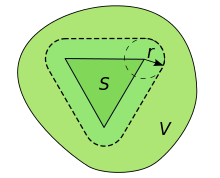
\includegraphics[scale=0.8]{images/Neighborhood_illust3.svg.png}
    \caption{r-neighborhood of the set $S$}
\end{figure}

\begin{definition}
    Let $(X,d)$ be a metric space, let $C \subset X$, we can define the \underline{distance from $x$ to $C$}:
    $$dist(x,C)=inf\{d(x,c):c \in C\}$$
\end{definition}

\begin{theorem}
    $$dist(x,C)-dist(y,C)\leq d(x,y)$$
\end{theorem}


\begin{definition}
    Let $f:(X,d_X)\longrightarrow (Y,d_Y)$. $f$ is called \underline{isometry} if it is a distance-preserving transformation between metric spaces.
    $$\forall a,b\in X.d_Y(f(a),f(b))=d_X(a,b)$$
\end{definition}

\begin{definition}
    A function $f:(X,d_X)\longrightarrow(Y,d_Y)$ is an \underline{isomorphism} if $f$ is an isometry and $f$
    is surjective. Two metric spaces are called \underline{isomorphic} if there is an isomorphism between them.
\end{definition}

\noindent \textbf{Remark}:
\begin{itemize}
    \item You can have a space that is a metric space, but not a vector space. Metric spaces do not need to have the notion of addition, or scaling. 
    \item It also can be the other way around as well. You can have a vector space that is not a metric space. Usually though we work with what are called normed vector spaces, which also have the notion of length of a vector. And these spaces induce a corresponding metric. (We talked about this in MAT247)
    \item All norms can be used to create a distance function as in $d(x,y)= \lVert x-y \rVert$, but not all distance functions have a corresponding norm.
\end{itemize}

\section{Metrics of $\R^n$}

\begin{definition}
    For the vector space $\R^n$, we can define the following norms to make different normed vector spaces. Let $x=(x_1,\cdots,x_n)\in \R^n$.
    \begin{itemize}
        \item We can define the \underline{Manhattan norm}:
        $$\lVert x \rVert_1=\sum_{j=1}^n|x_j|$$
        \item We can define the \underline{Euclidean norm}:
        $$\lVert x \rVert_2=\sqrt{\sum_{j=1}^nx_j^2}$$
        \item  We can define the \underline{Infinity norm}:
        $$\lVert x \rVert_{\infty}=sup\{|x_1|,\cdots,|x_n|\}$$
    \end{itemize}
\end{definition}


\begin{definition}
    For the vector space $\R^n$, the metrics derived from the previous norms are:
    \begin{itemize}
        \item \underline{Manhattan distance}: $$d_1(x,y)=|x_1-y_1| + \cdots +|x_n-y_n|$$
        \begin{figure}[ht]
            \centering
            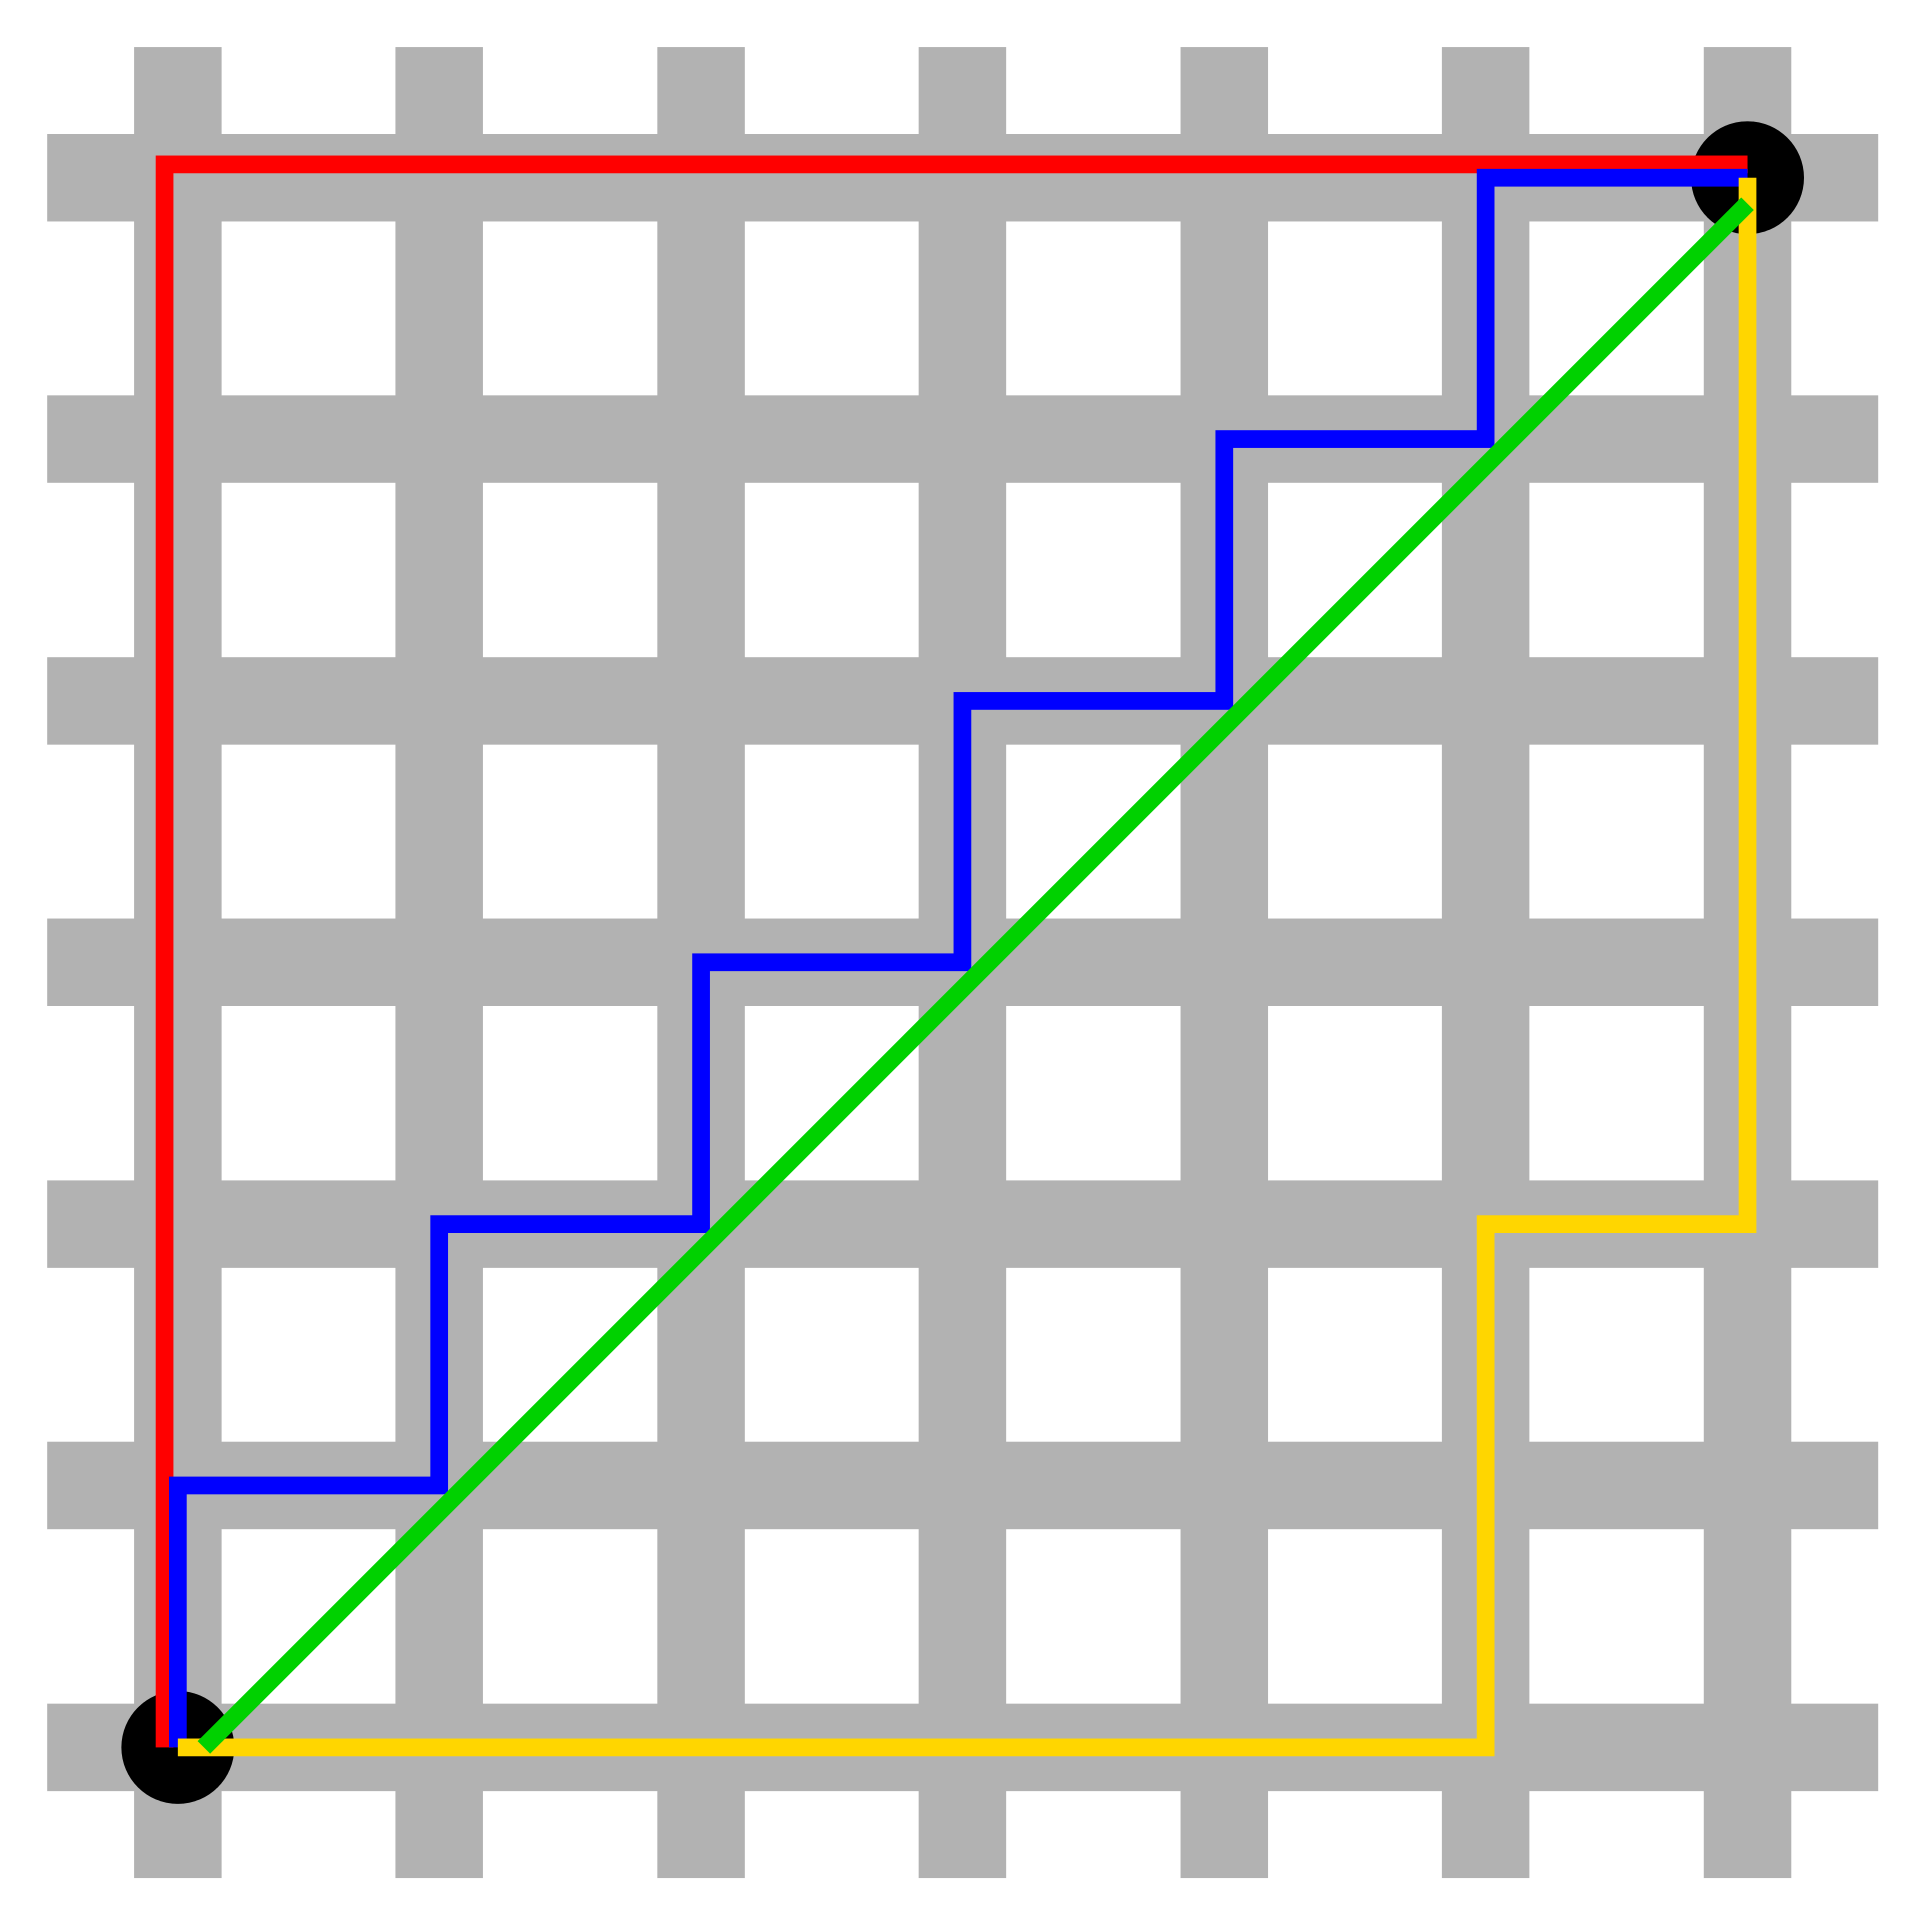
\includegraphics[scale=0.1]{images/Manhattan_distance.svg.png}
            \caption{A picture description of Manhattan distance}
        \end{figure}
        \item \underline{Euclidean distance}: $$d_2(x,y)=\sqrt{|x_1-y_1|^2+ \cdots |x_n - y_n|^2}$$
        The first and the second properties are clear. For the third property, it follows by Pythagoras theorem or Cauchy-Schwarz inequality.
        \item \underline{Chebyshev distance}: $$d_{\infty}(x,y)=sup\{|x_1-y_1|,\cdots ,|x_n-y_n|\}$$
    \end{itemize}
\end{definition}



\begin{lemma} \label{sup2eq}
    In $\R^n$ with the previous norms, we have
    $$\lVert x \rVert_{\infty} \leq \lVert x \rVert_2 \leq \sqrt{n} \lVert x \rVert_{\infty}$$
\end{lemma}


\begin{lemma} \label{21eq}
    In $\R^n$ with the previous norms, we have
    $$\lVert x \rVert_2 \leq \lVert x \rVert_1 \leq \sqrt{n} \lVert x \rVert_2$$
\end{lemma}

\begin{definition}
    In $\R^n$, let $a \in \R^n$ be arbitrary
\begin{itemize}
    \item the \underline{open cube} is $$C(a,\epsilon)=\{x \in \R^n: \lVert x-a \rVert_{\infty}<\epsilon\}$$
    \item the \underline{usual open ball} is just $$B(a;\epsilon)=\{x \in \R^n:  \lVert x-a \rVert_2<\epsilon\}$$
    \item the \underline{taxicab ball} i.e.manhattan ball is defined as $$T(a;\epsilon)=\{x \in \R^n:  \lVert x-a \rVert_1<\epsilon\}$$
\end{itemize}
\begin{figure}[h]
    \centering
    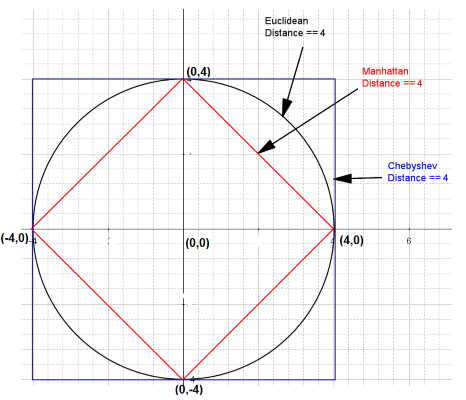
\includegraphics[scale=0.5]{images/FSnE9ZFXoAkp2Tp.png}
    \caption{Ball of radius 4 of the previous distance functions}
\end{figure}
\end{definition}

\begin{lemma}\label{CcontainsB}
    $$B(a;\epsilon) \subset C(a;\epsilon) \subset B(a;\sqrt{n}\epsilon)$$
\end{lemma}


\begin{lemma}
    $$T(a;\epsilon) \subset B(a;\epsilon) \subset T(a;\sqrt{n}\epsilon)$$
\end{lemma}

\begin{definition}
    Let $V$ be a vector space. Given $\lVert \cdot \rVert_a$ and $\lVert \cdot \rVert_b$ two norms on the vector space, we say $\lVert \cdot \rVert_a$ and $\lVert \cdot \rVert_b$ are \underline{equivalent} if there 
    exist positive constants $r_1,r_2$ such that for all $v \in V$ we have 
    $$r_1 \lVert x \rVert_a \leq \lVert x \rVert_b \leq r_2\lVert x \rVert_a$$
\end{definition}

\begin{theorem}
    $\lVert \cdot \rVert_1$ and $\lVert \cdot \rVert_2$ and $\lVert \cdot \rVert_{\infty}$ are equivalent.
\end{theorem}


\begin{theorem*}
    If the vector space is a finite-dimensional real or complex one, all norms are equivalent.
\end{theorem*}

\begin{theorem*} \label{topology induced by eq norms}
    The topologies induced by two equivalent norms are the same.
\end{theorem*}
\noindent \textbf{Remark}:
\begin{itemize}
    \item We are not going to prove this theorem right now, this only gives an intuition of why we study metric topology.
\end{itemize}

\section{Metric Topology}
We now know that the three norms defined on $\R^n$ will induce the same topology on $\R^n$. 
So the three different norms derive three different metric spaces. And the three metric spaces will have the same structure. 
In this chapter, we focus on the structure of $\R^n$, i.e. the topology of $\R^n$. Actually, we can start from any of the three metric spaces(usually we pick the Euclidean norm) to study the structure of $\R^n$.
Therefore the most important thing for now is to learn how to analyze the structure of the general metric space.
\begin{definition}
    Given any metric space $(X,d)$, an \underline{open set} is a subset $A \subset X$ such that $$\forall a \in A. \exists \epsilon >0. U(a;\epsilon) \subset A$$
\end{definition}
\noindent \textbf{Examples}:
\begin{itemize}
    \item The interval $(a,b)$ in $\R$ is an open set.
    \item The interval $(a,b]$ in $\R$ is not an open set because of the point $b$.
    \item $\bigcup_{n \geq 1}^{\infty}(\frac{1}{2^{n+1}},\frac{1}{2^n})$ is open.
    \item $\bigcap_{n \geq 1}^{\infty}(-\frac{1}{n},\frac{1}{n})=\{0\}$ is not an open set.
\end{itemize}
\noindent \textbf{Remark}:
\begin{itemize}
    \item An arbitrary union of open sets is open.
    \item A finite intersection of open sets is open.
    \item Can check that $\mathcal{B}_d=\{B(x;\epsilon):x\in X\text{ and }\epsilon>0\}$ can form a basis for $X$.
\end{itemize}

\begin{definition}
    Given a set $X$ and a metric $d$, The topology generated by the basis $\mathcal{B}_d=\{B(x;\epsilon):x\in X\text{ and }\epsilon>0\}$ is called the \underline{metric topology}.
\end{definition}

\begin{definition}
    If $U$ is any open set containing $x_0$, we commonly refer to U simply as a \underline{neighborhood of $x_0$}.
\end{definition}

\begin{definition}
    A set is closed if and only if it's complement is open.
\end{definition}
\noindent \textbf{Remark}:
\begin{itemize}
    \item Any intersection of closed sets is close.
    \item Finite union of closed sets is close.
\end{itemize}

\begin{lemma}
    Let $(X,d)$ be a metric space, let $Y \subset X$. Then 
    $$A \subset Y \text{ is open in }Y \Longrightarrow A=Y\cap U \text{ for some open }U \text{ in }X.$$
\end{lemma}


\begin{definition}
    Given any subset $A \subset X$, a point $x \in A$ is a \underline{limit point} of $A$ if 
    $$\forall \epsilon >0. \exists x' \in A. x' \neq x \text{ and }x' \in U(x;\epsilon)$$
\end{definition}
\noindent \textbf{Example}:
\begin{itemize}
    \item For the interval $[0,1)$, 0 is a limit point and 1 is a limit point.
\end{itemize}
\noindent \textbf{Remark}:
\begin{itemize}
    \item In any metric space $(X,d)$ with the metric topology, if $x_0$ is a limit point of $Y \subset X$, then
    $$\forall \epsilon >0. \exists \text{ infinitely many }x_1 \in U(x_0;\epsilon). x_1 \in Y$$
    \underline{A finite set in metric space has no limit points.}\\
    Because each point $p$ has a positive distance to the points of the set (other than itself if it is a member of the set), 
    and since there are finitely many of them, there is a minimum distance $d$. The open ball of radius $d$ around $p$ doesn't contain any elements of the set other than $p$.
    \item The statement is not true when we generalize to topological spaces. 
    For example, $$X=\{1,2,3\}, \mathcal{T}=\{\emptyset,\{1,2\},\{1,3\},\{2,3\},\{1,2,3\}\}$$
    the set $\{1,2\}$ has limit point 3.
\end{itemize}

\begin{theorem}
    A set $A \subset X$ is closed if and only if it contains all it's limit points.
\end{theorem}

\begin{definition}
    Let $(X,d)$ be a metric space, let $A \subset X$, we define the \underline{closure} of $A$:
    $$\overline{A}=A \cup \{\text{all limit points of } A\}$$
\end{definition}

\begin{lemma}
    $$\overline{A}=\bigcap \{\text{closed sets containing $A$}\}$$
\end{lemma}

\begin{definition}
    Given any set $A \subset X$, the \underline{interior} of $A$ is 
    $$Int(A)=\bigcup \{\text{all open sets contained in $A$}\}$$
\end{definition}

\begin{definition}
    Given any set $A \subset X$, the \underline{exterior} of $A$ is 
    $$Ext(A)=\bigcup \{\text{all open sets contained in $A^C$}\}$$
\end{definition}

\begin{definition}
    Given any set $A \subset X$, the \underline{boundary} of $A$ is 
    $$Bd(A)= X\setminus(Int(A) \cup Ext(A))$$ 
    some books will use the notation $\partial A$.
\end{definition}

\section{Continuity in Metric Space}

\begin{definition}
    Let $(X,d),(Y,h)$ be metric spaces. Construct a function $f:X \longrightarrow Y$ over a subset $A \subset X$. 
    $$f:A \longrightarrow Y$$
    Let $x_0 \in A$, we say $f$ is \underline{continuous at $x_0$} iff 
    $$\forall \text{open $V \subset Y$ containing $f(x_0)$ }. \exists \text{open }U \subset X \text{ containing }x_0. f(U) \subset V $$
    We can use $\epsilon - \delta$ language to express the definition clearly:
    \begin{itemize}
        \item $\forall \epsilon>0. \exists \delta >0. \forall x \in A. x \in U(x_0;\delta) \Longrightarrow f(x) \in V(f(x_0);\epsilon)$ where $V$ is open ball in $(Y,h)$.
        \item $\forall \epsilon>0. \exists \delta >0. \forall x \in A. d(x;x_0)<\delta \Longrightarrow h(f(x);f(x_0))<\epsilon$.
    \end{itemize}
\end{definition}

\begin{definition}
    We say $f$ is \underline{continuous} if it is continuous at each point $x_0$ of $A$.
\end{definition}

\begin{theorem}
    A map $f:(X,d) \longrightarrow (Y,h)$ is continuous if and only if the preimage of every open subset is open.
    $$\forall V \subset Y \text{ open. } f^{-1}(V) \text{ is open in }X$$
\end{theorem}


\noindent \textbf{Examples}:
\begin{itemize}
    \item Let $X=\R^3$, $Y$ be any set. $A=\{(0,0,0),(0,\sqrt{2},-\sqrt{3}),(e,\pi,e^{\pi})\}$,\\ then $f:A \longrightarrow Y$ is continuous.\\
    First, we claim that \underline{any subset of $A$ is open}.
    \begin{proof}
        Let $x_0 \in A$ be arbitrary, $x_0$ is the only element in $\{x_0\}$. 
        Let $\epsilon=min\{d(x_0,x_1),d(x_0,x_2)\}$, then $U(x_0,\epsilon)=\{x_0\} \subset \{x_0\}$. 
        So $\{x_0\}$ is open. Any subset of $A$ is the union of singletons, hence is open.
    \end{proof}
    Fix $x_0$, let $U \subset Y$ be an open set that contains $f(x_0)$. 
    By the claim above, $f^{-1}(U)$ is open. So $f$ is indeed continuous. 
    More generally, if $A$ is finite, then $f:A \longrightarrow Y$ is continuous.
    \item Let $A=\overline{U(x_0,1)}\cup \{p_1,\cdots,p_n\}$ with all $p_i \notin \overline{U(x_0;1)}$\\
    Suppose $f:\overline{U(x_0;1)} \longrightarrow Y$ is continuous, then $f:A \longrightarrow Y$ is continuous.\\
    \underline{In MAT157, we knew that $f$ is continuous on isolated points.}
\end{itemize}

\begin{theorem} \label{dist continuous}
    Let $(X,d)$ be a metric space, fix a subset $C$ in the metric space $X$.
    Then the function $$dist:X \longrightarrow \R$$ is continuous.
\end{theorem}

\begin{definition}
    $f:(X,d) \longrightarrow (Y,h)$ is \underline{uniformly continuous} if 
    $$\forall \epsilon >0. \exists \delta >0. \forall x,y \in X.d(x,y)<\delta \Longrightarrow h(f(x),f(y))<\epsilon$$
\end{definition}
\noindent \textbf{Examples}: functions which are continuous but not uniformly continuous.
\begin{itemize}
    \item $f:[0,\infty) \longrightarrow \R,f(x)=x^2$
    \item $f:(0,1) \longrightarrow \R,f(x)=\frac{1}{x}$
\end{itemize}

\section{Compactness in Metric Space}

\begin{definition}
    Let $(X,d)$ be a metric space, $Y \subset X$ ,an \underline{open cover} of $Y$ is a collection of open sets $U_\alpha,\alpha \in A$, such that $$Y \subset \bigcup_{\alpha \in A}U_{\alpha}$$
\end{definition}

\begin{definition}
    Let $(X,d)$ be a metric space, a subset $Y \subset X$ is \underline{compact} if any open cover of $Y$ has a finite subcover.
    Suppose $U_{\alpha},\alpha \in A$ is an open cover of $Y$, $Y$ is compact if there exists a finite collection $\alpha_1,\cdots,\alpha_n \in A$ such that $$Y \subset \bigcup_{i=1}^n U_{\alpha_i}$$
\end{definition}
\noindent \textbf{Example}:
\begin{itemize}
    \item In $\R$, the interval $[a,b]$ is compact.
\end{itemize}

\begin{theorem}
    Every closed subspace of a compact space is compact.
\end{theorem}

\begin{theorem}\label{compactimpliesclosedbounded}
    If $Y \subset (X,d)$ is compact, then $Y$ is closed and bounded.
\end{theorem}

\begin{theorem} \label{lemmaevt}
    Let $f:(X,d) \longrightarrow (Y,h)$ be a continuous function. If $A$ is compact in $X$, then $f(A)$ is compact in $Y$.
\end{theorem}

\begin{corollary}[Extreme Value Theorem] \label{evt}
    Let $f:A \subset X \longrightarrow \R$ be a continuous function. If $A$ is compact, then $f(A)$ has a maximum value and a minimum value.
\end{corollary}

\begin{theorem}[The $\epsilon$-neighborhood Theorem] \label{epsilon neighborhood thm}
    Let $(X,d)$ be a metric space, consider a compact set $Y \subset X$ and an open set $U$ containing $Y$. 
    Then there exists $\epsilon>0$ such that an $epsilon$-neighborhood of $Y$ is contained in $U$.
\end{theorem}

\begin{theorem}\label{continuous function on compact set is uniformly continuous}
    If $(X,d)$ and $(Y,h)$ be metric spaces, let $X$ be compact and $f:X \longrightarrow Y$ continuous. 
    Then $f$ is uniformly continuous.
\end{theorem}



\begin{theorem}\label{rectanglecompact}
    The rectangle $Q=[a_1,b_1]\times \cdots \times [a_n,b_n] \subset \R^n$ is compact.
\end{theorem}


\begin{definition}
    a topological space X is \underline{sequentially compact} if every sequence of points in $X$ has a convergent subsequence converging to a point in $X$.
\end{definition}

\begin{theorem}
    In metric space, compactness is equivalent to sequentially compactness.
\end{theorem}

\section{Connectedness in  Metric Space}

\begin{definition}
    Let $(X,d)$ be a metric space, we say $X$ is \underline{connected} if $X$ cannot be written as the union of two disjoint non-empty sets $A$ and $B$, each of which is open in $X$.
\end{definition}

\begin{theorem}
    The real line $\R$ is connected and so are the intervals and rays.
\end{theorem}

\begin{theorem}
    Let $(X,d)$ be a connected metric space, if $f:X \longrightarrow Y$ is continuous, then $f(X)$ is connected in $Y$.
\end{theorem}

\begin{corollary}[Intermediate-Value Theorem]
    Let $(X,d)$ be a metric space and $f:X \longrightarrow \R$ is continuous, then if $f(x_0) < r < f(x_1)$ for some points $x_0,x_1$ of $X$,then $f(x)=r$ for some point $x$ of $X$.
\end{corollary}

\begin{definition}
    Let $a,b$ be two points in $\R^n$, the \underline{line segment} joining $a$ and $b$ is:
    $$\{a+t(b-a): t\in [0,1]\}$$
\end{definition}
\begin{figure}[ht]
    \centering
    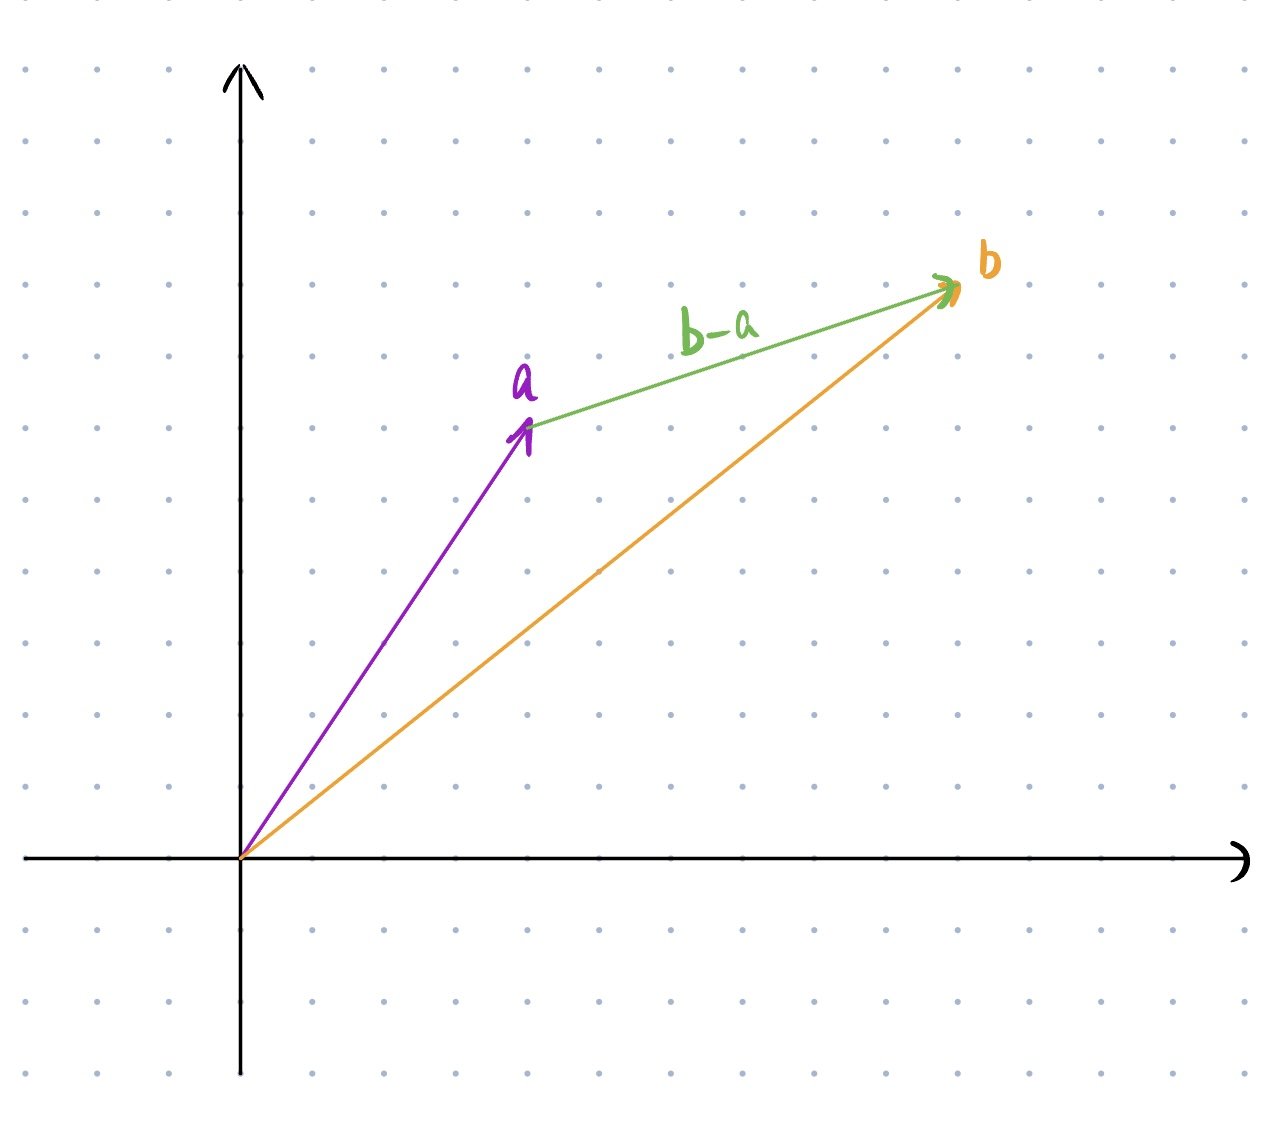
\includegraphics[scale=0.17]{images/line_segment.jpg}
    \caption{the line segment joining a and b}
\end{figure}

\begin{definition}
    A subset $A \subset \R^n$ is \underline{convex} if $\forall a,b \in A$, the line segment joining $a$ and $b$ is contained in $A$.
\end{definition}

\begin{theorem}
    Open balls and open cubes in $\R^n$ are convex.
\end{theorem}

\begin{theorem}
    Open rectangles and closed rectangles in $\R^n$ are convex.
\end{theorem}
\chapter{Differentiation}

\section{The Derivative}

\begin{definition}
    The \underline{derivative} of a single variable function $f:A\subset \R \longrightarrow \R$ 
    at the point $a\in A$ given $a \in U(a;\epsilon)$ is 
    $$f'(a)=\lim_{h \to 0}\frac{f(a+h)-f(a)}{h}$$
\end{definition}

\noindent \textbf{Remark}: Realizations regarding the derivative of a single variable function:
\begin{enumerate}
    \item Newton: Rate of change of the function at the point $a$ is equal to the derivative of it at $a$
    $$x(t)\longrightarrow x'(t)=v(t):\text{velocity at }t$$
    \item Leibnitz: Realize the graph of $f$, the derivative of $f$ at $a\in A$ is the slope of the line tangent to the graph of $f$ at $(a,f(a))$.
    \item Taylor: The best linear approximation of $f(x)$ near $a$ is given by $$L(a+h)=f(a)+hf'(a)$$
    We can prove that $$r(h):=f(a+h)-L(a+h)\text{ satisfies } \lim_{h \to 0}\frac{r(h)}{h}=0$$
\end{enumerate}

\begin{definition}
    Let $f:A\subset \R^m \longrightarrow \R^n$. The \underline{directional derivative} of $f$ at the point $a\in A\subset \R^m$ with respect to the unit vector $u\in \R^n$ is defined as:
    $$D_uf(a)=\lim_{h \to 0}\frac{f(a+hu)-f(a)}{h}$$
    some books will adopt the notation $\nabla_uf(a)$, the symbol is called nabla or del.
\end{definition}
\begin{figure}[ht]
    \centering
    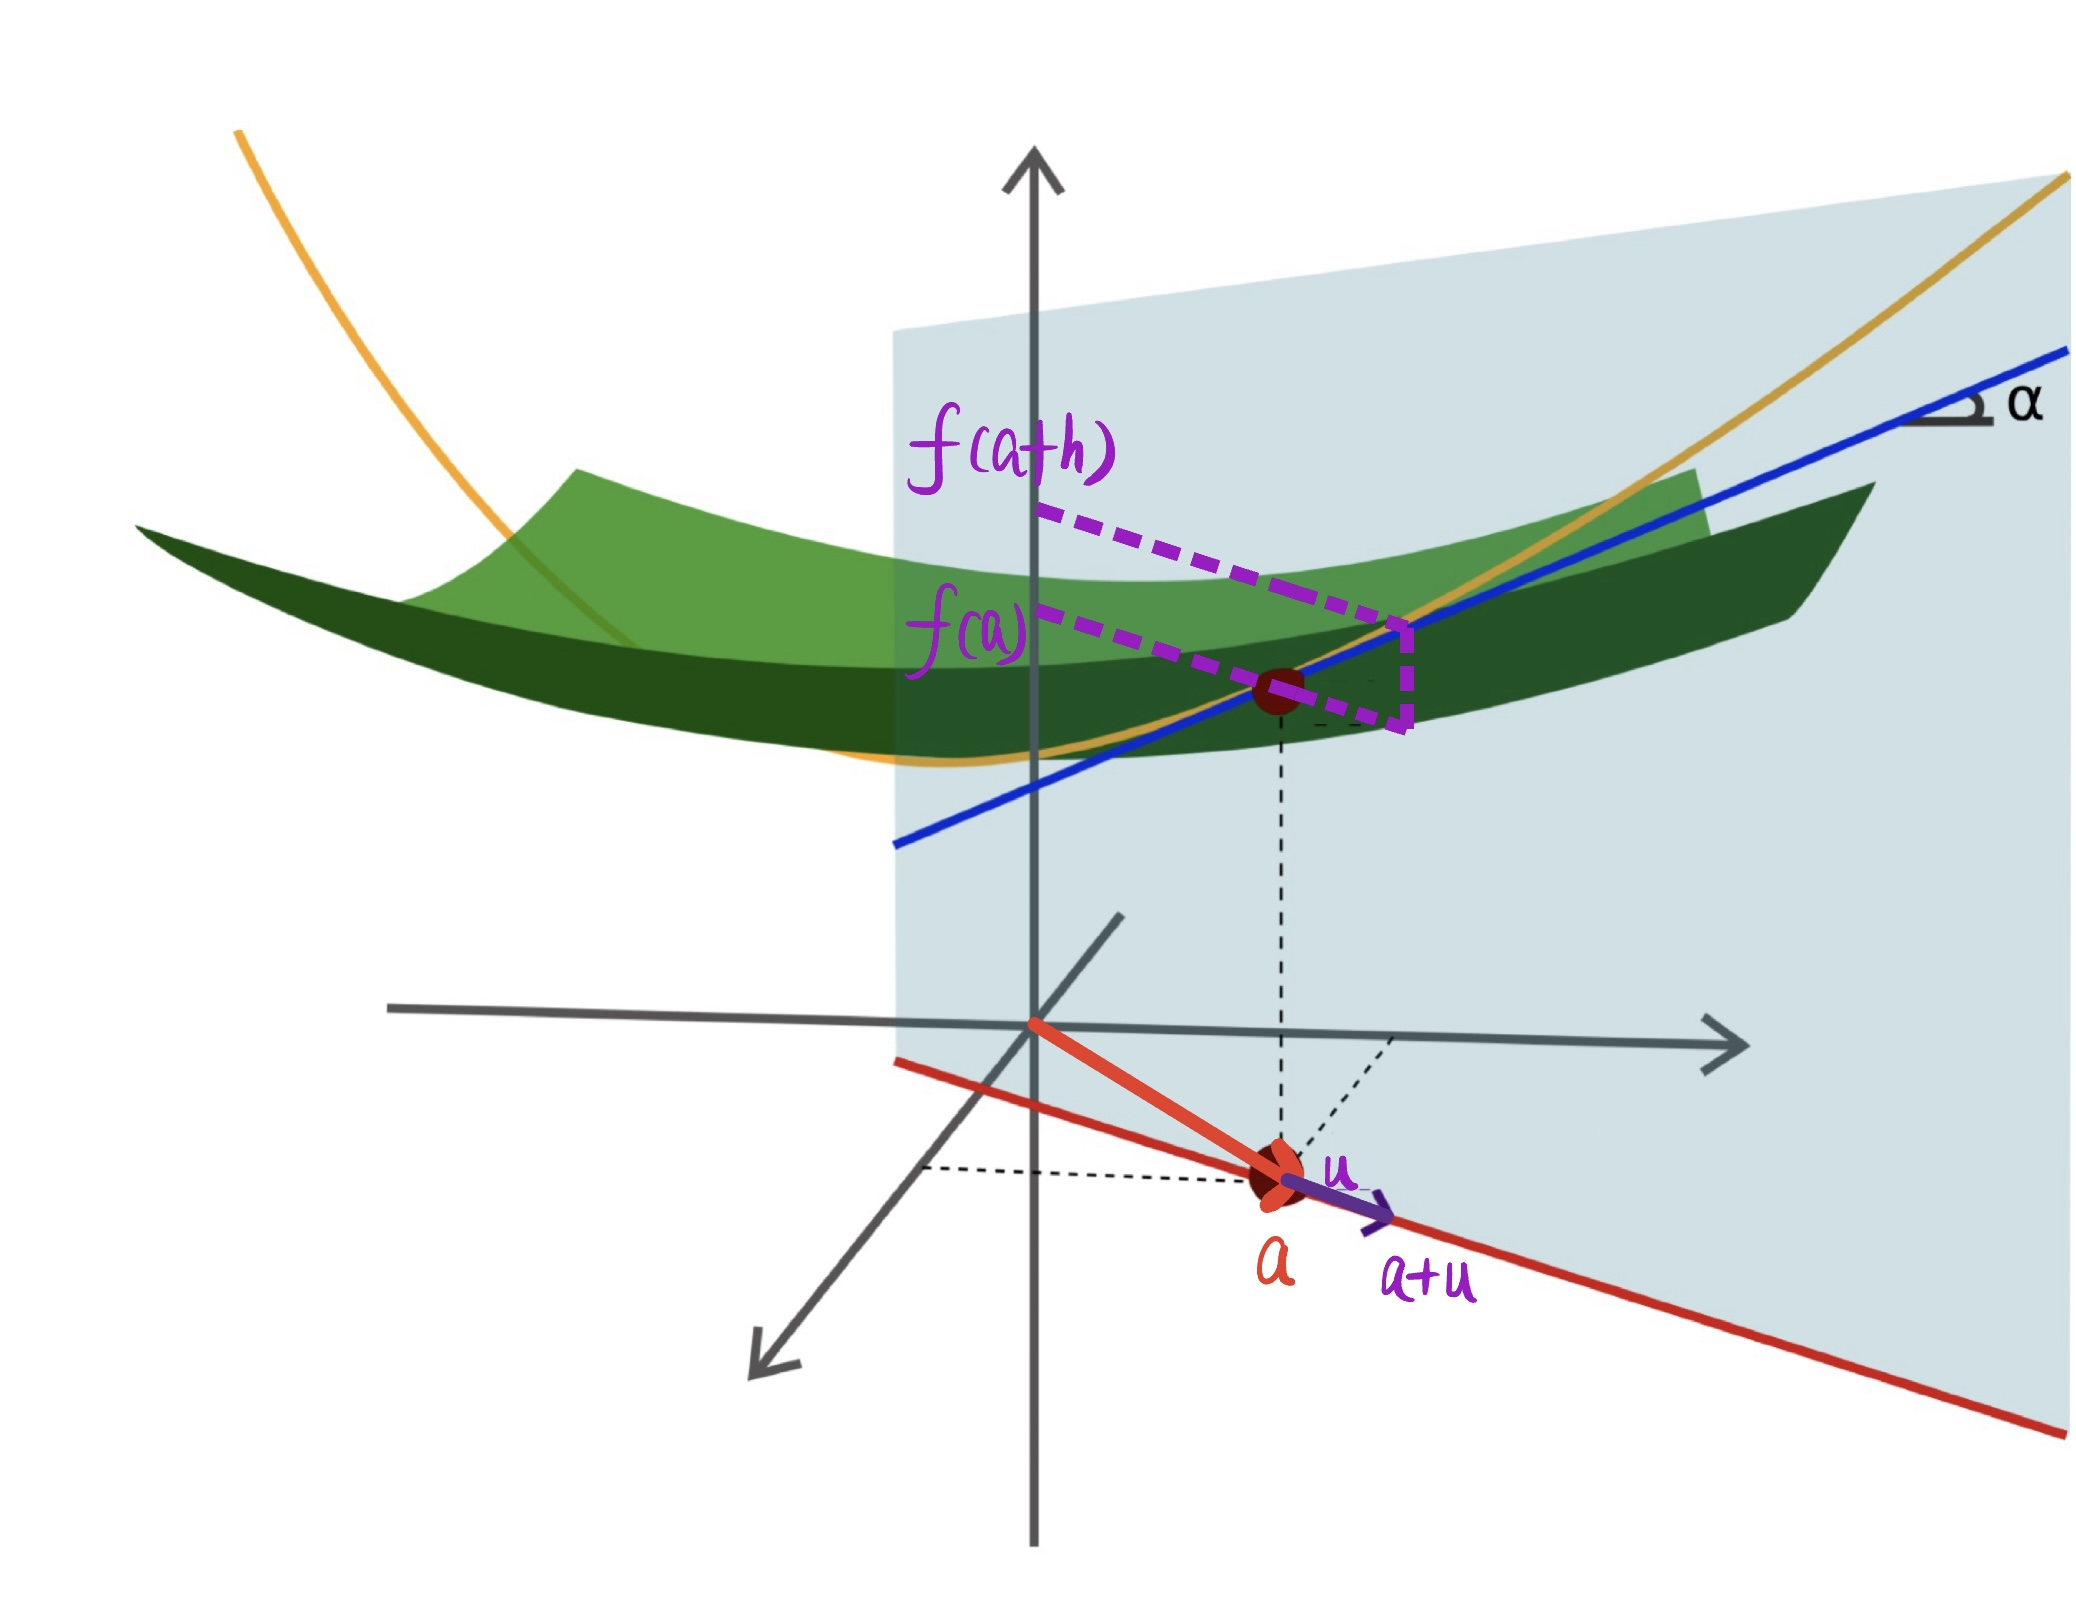
\includegraphics[scale=0.17]{images/IMG_0326.jpg}
    \caption{A picture description of directional derivative}
\end{figure}
\noindent \textbf{Remark}:
\begin{itemize}
    \item For $f:A \subset \R^2 \longrightarrow \R$, the directional derivative of the point $a$ given the unit vector $u$ is described in the picture. 
    Essentially, we are focusing on the plane in which the point $a$ and the unit vector $u$ are located. The set $f(A)$ on the plane is just a curve, if we think the unit vector $u$ as the unit vector for the $x$-axis on our new plane, then we can calculate the line tangent to $(a,f(a))$ as usual.
    \item But our purpose is to find a linear approximation near the point $a$, if we just use the directional derivative, then the linear approximation we get is the line tangent to $(a,f(a))$ on the plane, this is clerly not enough. Intuitively, for $f:A \subset \R^2 \longrightarrow \R$, 
    the best linear approximation near a point $a\in A$ should be a plane tangent to $(a,f(a))$ instead of a line.
    So assume $L:\R^2 \longrightarrow \R$ is the best linear approximation for the function $f$, we must have $$L(a+h)=f(a)+B\cdot h$$
    $B$ must be a map from $\R^2$ to $\R$, hence it should be a 1 by 2 matrix.
\end{itemize}

\noindent \textbf{Example}:
\begin{itemize}
    \item As we are familiar with all concepts of differentiation and integration of functions from $\R$ and $\R^2$ to $\R$ in high school physics. Let us consider a fuction $f:\R^2 \longrightarrow \R^2$ defined as 
    \begin{align}
        f(\begin{bmatrix}
               x \\
               y \\
        \end{bmatrix}) = 
        \begin{bmatrix}
            x+sin(y) \\
            y+sin(x) \\
        \end{bmatrix}
    \end{align}
    If we use grids to visualize the transformation $f$, we can see clearly that $f$ is not linear. But this function has a nice property, which we called \underline{locally linear}.
    If we zoom in on a given point, we can see this looks a lot more like a linear function. And the more we zoom in, the more it looks precisely like a linear function.
    \begin{figure}[ht]
        \centering
        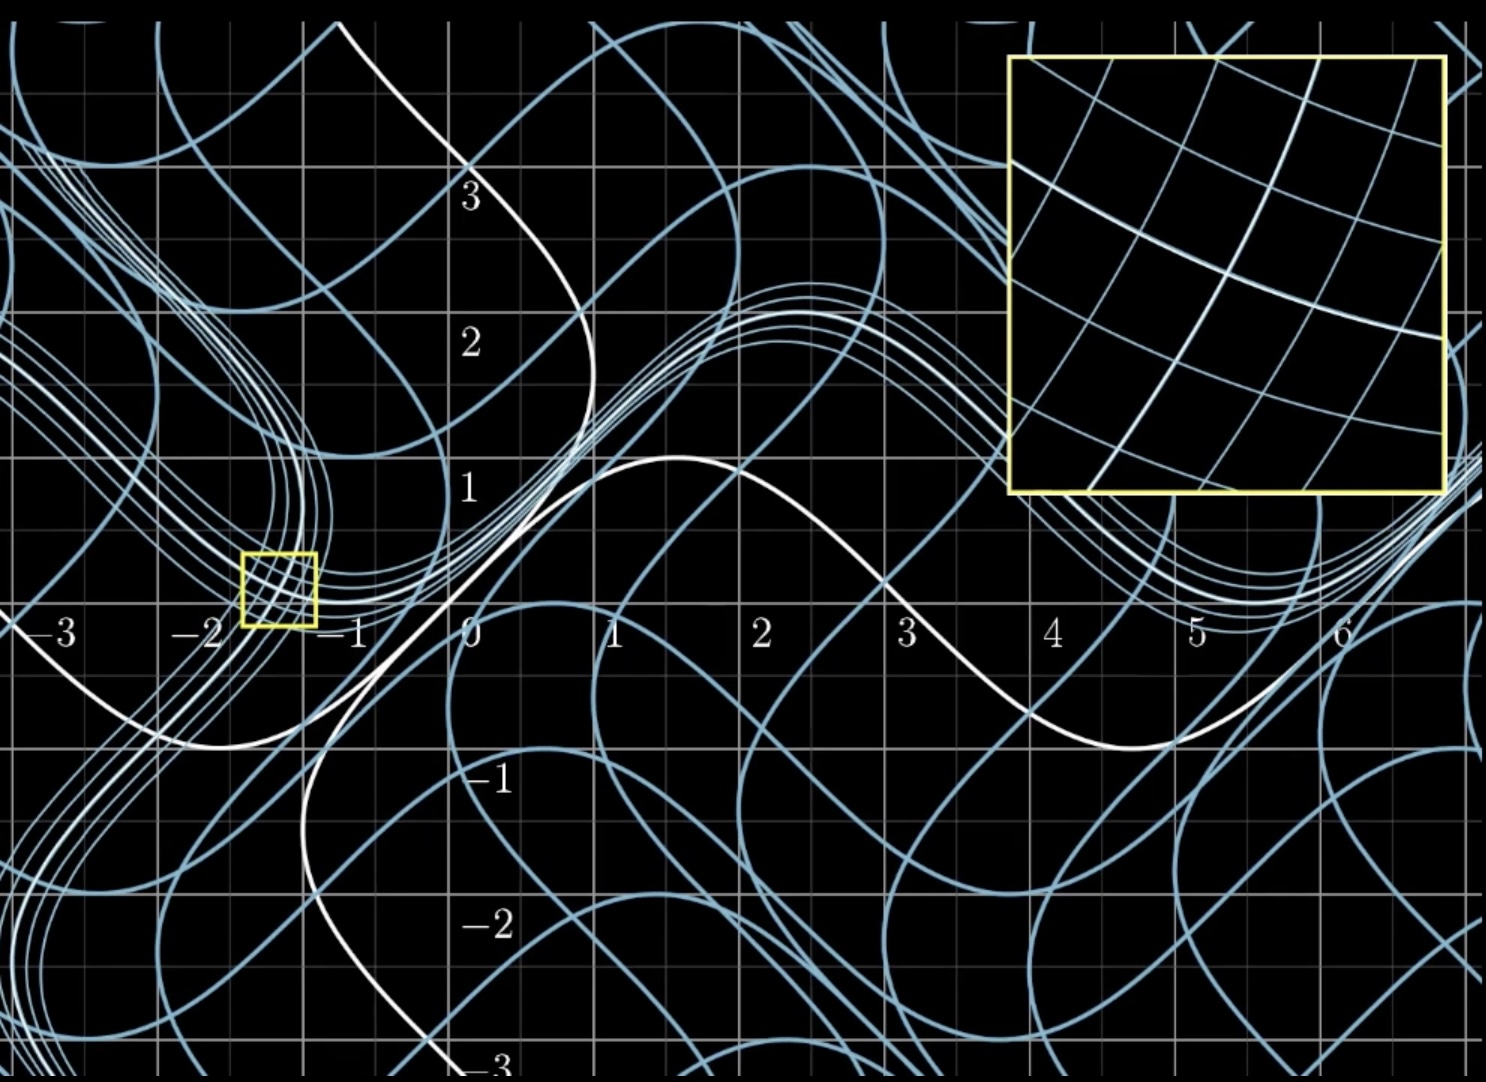
\includegraphics[scale=0.4]{images/locallylinear.jpg}
        \caption{Zoom in on a given point}
    \end{figure}
    So it is our desire to make the linear approximation on the given point $a$. Still, let $L:\R^2\longrightarrow \R^2$ be the best linear approximation, we must have 
    $$L(a+h)=f(a)+B\cdot h$$
    where $B$ should be the 2 by 2 matrix represent the linear transformation that the complicated function $f$ looks like around the point $a$.
\end{itemize}


\begin{definition}
    Let $f:A \subset \R^m \longrightarrow \R^n$. Suppose $A$ contains a neighborhood of $a$. We say that $f$ is \underline{differentiable at $a$} if there is an n by m matrix $B$ such that
    $$\lim_{\lVert h \rVert \to 0}\frac{\lVert f(a+h)-f(a)-B\cdot h \rVert}{\lVert h \rVert}=0$$
    The matrix $B$, which is unique, is called the \underline{(total) derivative} or the \underline{jacobian matrix} of $f$ at $a$, denoted as $Df(a)$.
\end{definition}

\begin{theorem}[Equivalent definition of the derivative]
    Let $f:A \subset \R^m \longrightarrow \R^n$. Suppose $A$ contains a neighborhood of $a$, if there is an n by m matrix $B$ such that
    $$\forall u \in \R^m. \lVert u \rVert =1 \Longrightarrow \lim_{t \to 0}(\frac{f(a+tu)-f(a)}{t}-B\cdot u)=0$$
    then the matrix $B$ is the derivative of $f$ at $a$.
\end{theorem}

\begin{theorem}[Uniqueness of the jacobian matrix]
    Suppose the matrix $B$ and the matrix $\tilde{B}$ both satisfy the equation above, then $B=\tilde{B}$.
\end{theorem}


\begin{theorem}
    Let $f:A\subset\R^m\longrightarrow\R^n$, if $f$ is differentiable at $a$, then $f$ is continuous at $a$.
\end{theorem}

\begin{theorem} \label{directional derivative from jmatrix}
    If the function $f:A \subset \R^m \longrightarrow \R^n$ is differentiable at the point $a$, then all the directional derivatives of $f$ at $a$ exist and $$D_uf(a)=B\cdot u$$
\end{theorem}
\noindent \textbf{Remark}:
\begin{itemize}
    \item The directional derivatives are uniquely calculated when $u \in \{e_1,\cdots,e_m\}$.
    \item However, the existence of all the directional derivatives does not guarantee that a function is differentiable at a point. For example,
    \begin{equation}
        f(x,y)=
        \begin{cases}
            \frac{x^2y}{x^4+y^2}& \text{ if } (x,y)\neq \vec{0}\\
            0& \text{ if otherwise}
        \end{cases}
    \end{equation}
    \begin{figure}[ht]
        \centering
        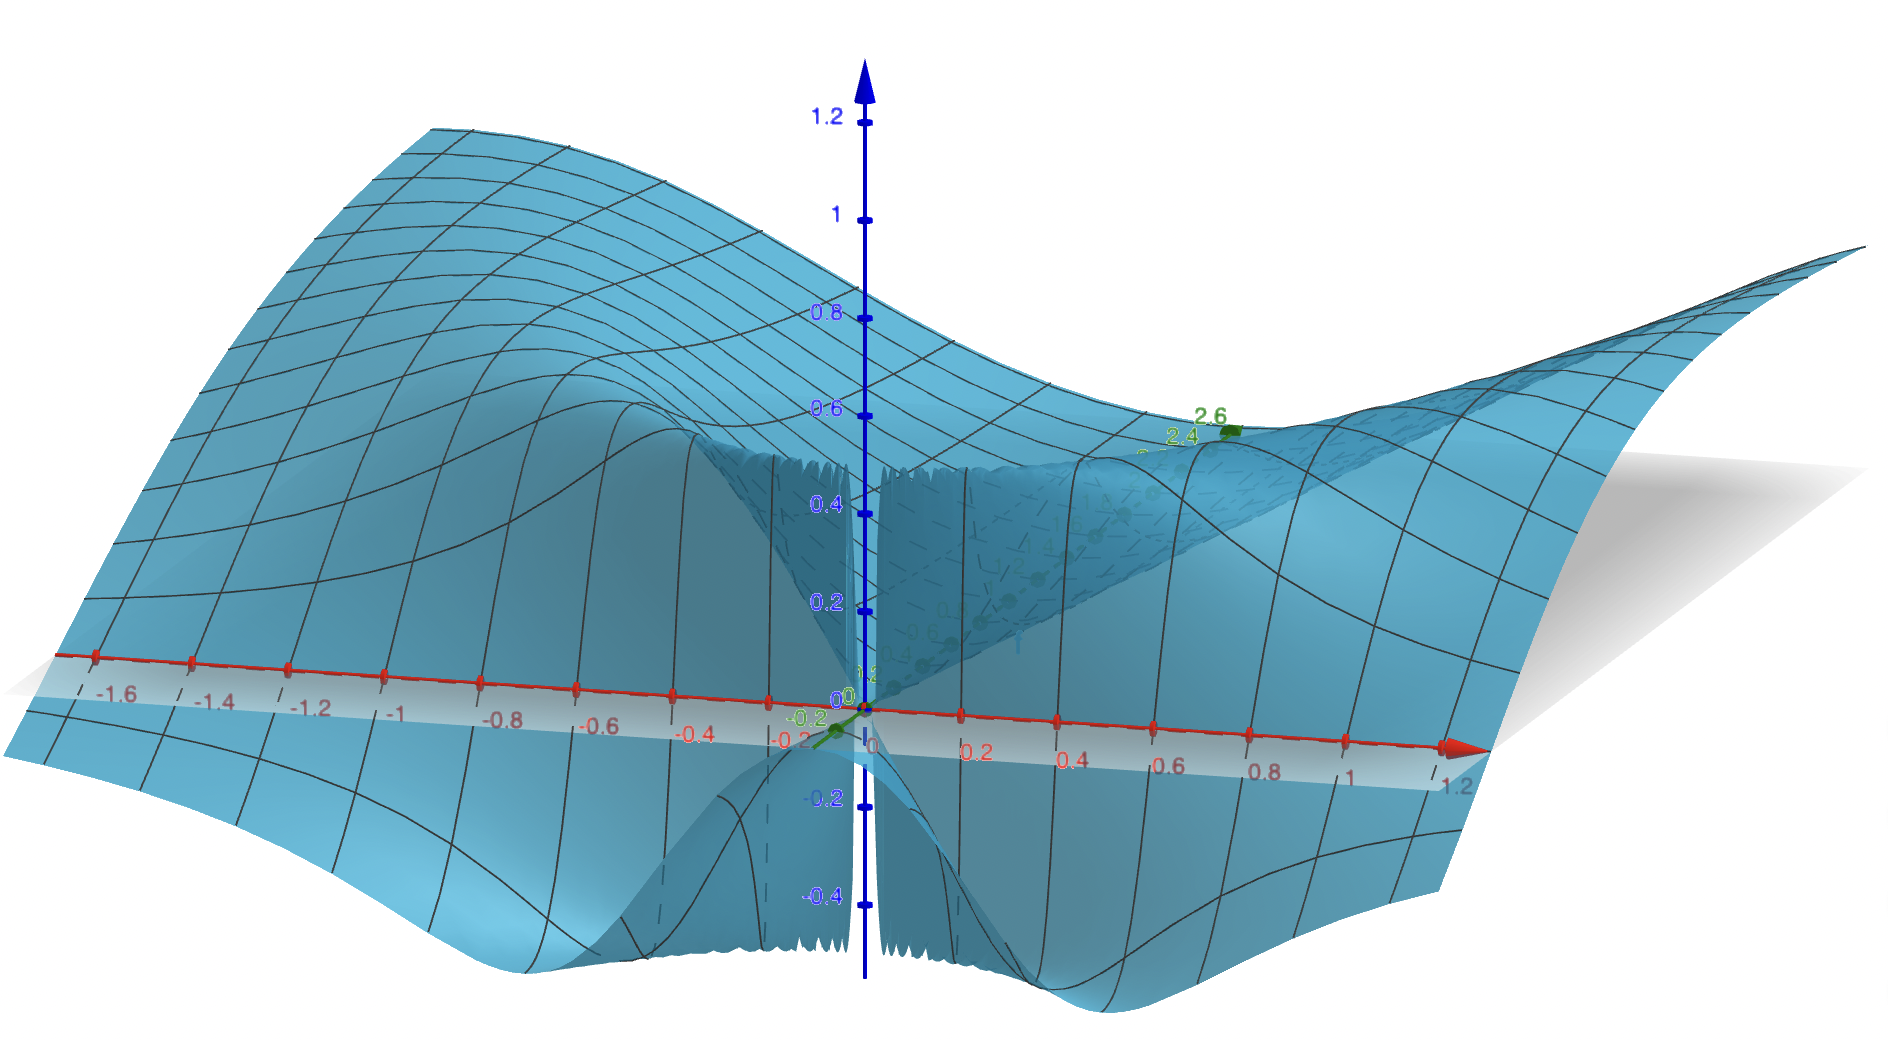
\includegraphics[scale=0.3]{images/Screen Shot 2022-09-29 at 11.44.44.png}
        \caption{$f(x,y)=\frac{x^2y}{x^4+y^2} \text{ if } (x,y)\neq \vec{0}$}
    \end{figure}
    $f$ is not differentiable at $(0, 0)$, but all of the directional derivatives exist at this point.\\
    Let $u=(h,k)\neq \vec{0}$, then
    \begin{equation}
        \begin{split}
            \frac{f(0+tu)-f(0)}{t} &= \frac{f(tu)}{t}\\
            &= \frac{(th)^2(tk)}{(th)^4+(tk)^2}\cdot \frac{1}{t}\\
            &= \frac{h^2k}{t^2h^4+k^2}
        \end{split}
    \end{equation}
    Taking the limit we have
    \begin{equation}
        \begin{split}
            D_uf(0)=\lim_{t\to 0}\frac{f(0+tu)-f(0)}{t} = \lim_{t\to 0}\frac{h^2k}{t^2h^4+k^2}
            &= \begin{cases}
                0\text{ }k=0\\
                \frac{h^2}{k}\text{ }k\neq0
            \end{cases}
        \end{split}
    \end{equation}
    We can see clearly that all directional derivatives around point 0 exist.\\
    Now we assume that $f:\R^2\longrightarrow \R$ is differentiable at $\vec{0}$. Then for some $a,b\in \R$
    $$Df(0)=\begin{bmatrix}
        a & b
    \end{bmatrix}$$
    $$Df(0)\cdot u=\begin{bmatrix}
    a & b
\end{bmatrix}\cdot u=ah+bk=D_uf(0)$$
This is a contradiction because we showed that $D_uf(0)$ is not linear.
\end{itemize}

\begin{definition}
    Let $f:A \subset \R^m \longrightarrow \R$ and $\{e_1,\cdots,e_m\}$ be the basis of $\R^m$, we define the \underline{j-th partial derivative} of $f$ at $a$ to be the directional derivative of $f$ at $a$ with respect to the vector $e_j$.
    $$D_jf(a):=D_{e_j}f(a)=\lim_{t \to 0}\frac{f(a+te_j)-f(a)}{t}$$
\end{definition}

\begin{lemma}\label{lemmajmatrix}
    Let $f:A \subset \R^m \longrightarrow \R$ be a function differentiable at $a$ and $\{e_1,\cdots,e_m\}$ be the basis of $\R^m$, then
    $$Df(a)=[D_1f(a)\cdots D_mf(a)]$$
\end{lemma}

\noindent \textbf{Example}:
\begin{itemize}
    \item Consider the function $f:\R^2\longrightarrow\R$, it can be presented as a 3-d picture.
    \begin{figure}[ht]
        \centering
        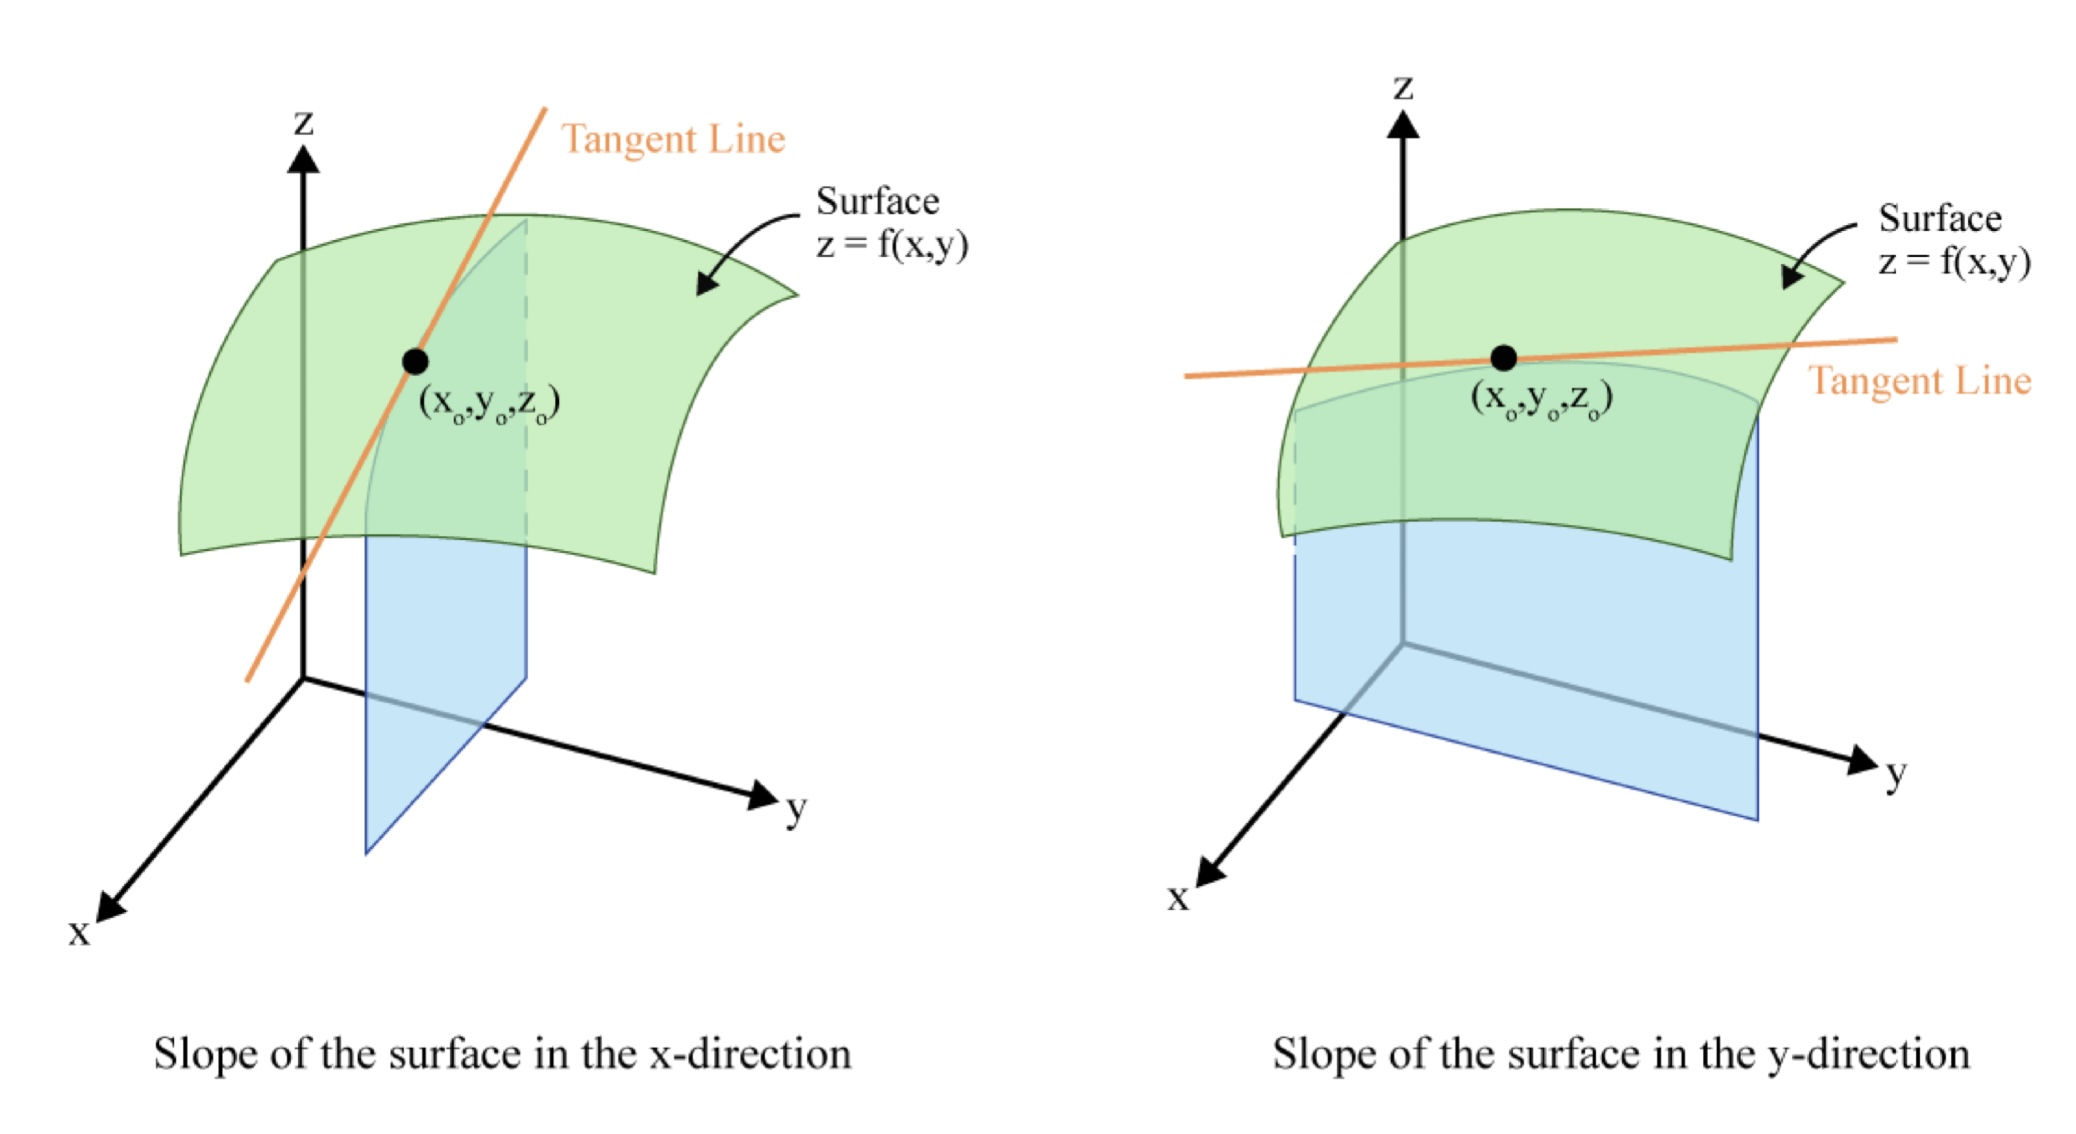
\includegraphics[scale=0.2]{images/IMG_0320.jpg}
        \caption{Partial derivative of $f:\R^2\longrightarrow \R$}
    \end{figure}
    \item Consider the function $f:\R^3\longrightarrow \R$. For $x\in \R^3$, the derivative is the row matrix
    $$Df(x)=\begin{bmatrix}
        D_1f(x)&D_2f(x)&D_3f(x)
    \end{bmatrix}$$
    In MAT240, we learnt that $Df(x)\in \mathcal{L}(\R^3,\R)$ and $\mathcal{L}(\R^3,\R)$ is a vector space of dimension $3$
    $$Df(x)=D_1f(x)\begin{bmatrix}
        1&0&0
    \end{bmatrix}+D_2f(x)\begin{bmatrix}
        0&1&0
    \end{bmatrix}+D_3f(x)\begin{bmatrix}
        0&0&1
    \end{bmatrix}$$
    Define the \underline{gradient} of $f$:
    $$\nabla f(x)=D_1f(x)e_1+D_2f(x)e_2+D_3f(x)e_3$$
    Now $\nabla f(x)$ is a vector in $\R^3$. And intuitively, \underline{it tells us the direction of the steepest increase of $x$}.
    \begin{figure}[ht]
        \centering
        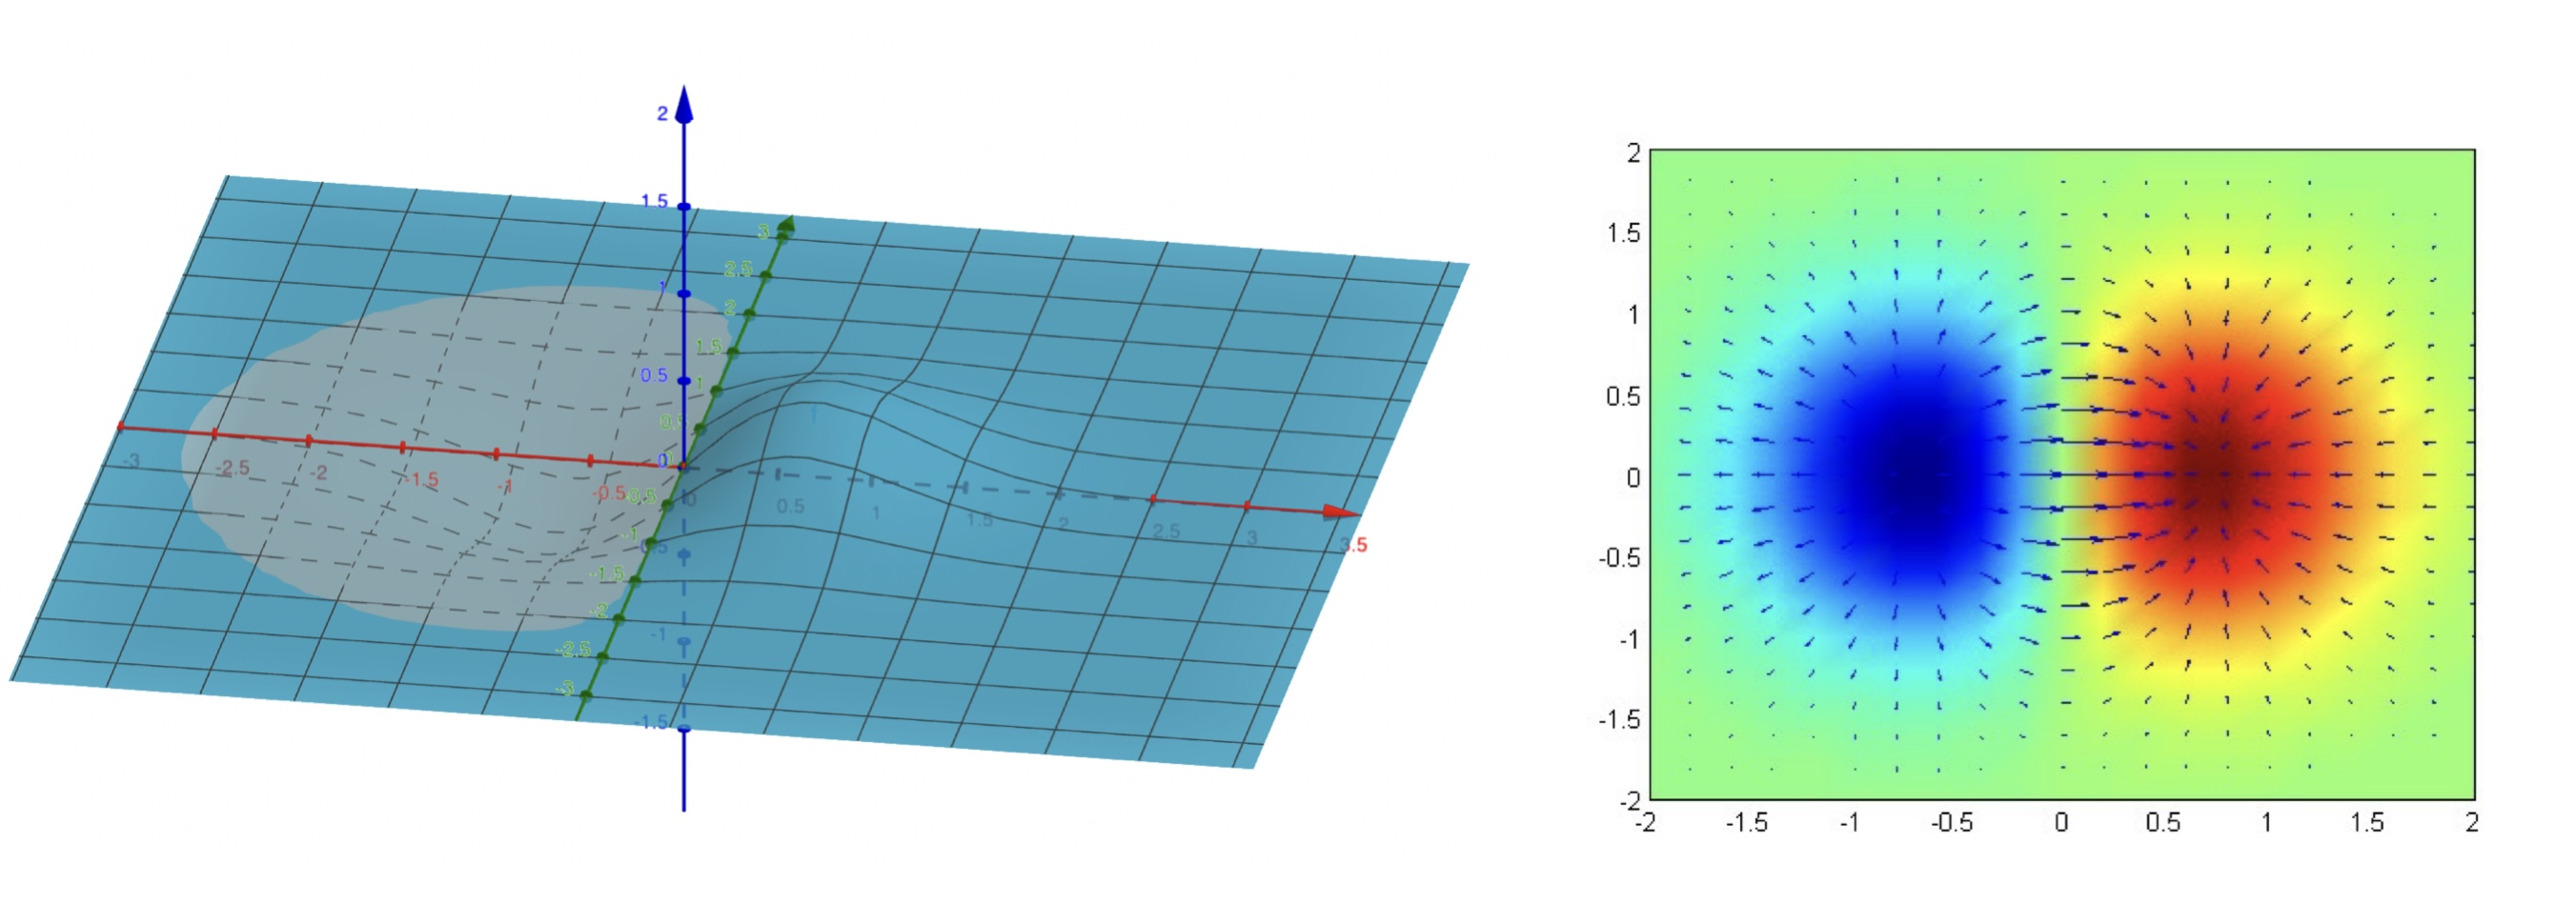
\includegraphics[scale=0.15]{images/IMG_0327.jpg}
        \caption{the gradient of $f(x,y)=xe^{-(x^2+y^2)}$}
    \end{figure}
\end{itemize}


\begin{definition}
    Let $f:A \subset \R^m \longrightarrow \R^n$, let $f_i:A\subset \R^m \longrightarrow \R$ be the \underline{i-th component function of $f$} such that
    \begin{align}
        f(a)=\begin{bmatrix}
            f_1(a)\\
            \vdots\\
            f_n(a)
        \end{bmatrix}
    \end{align}
\end{definition}

\begin{theorem} \label{differentiable iff components differentiable}
    The function $f$ is differentiable at $a$ if and only if each component function $f_i$ is differentiable at $a$.
\end{theorem}

\begin{theorem*} \label{continuous iff components continuous}
    The function $f$ is continuous at $a$ if and only if each component function $f_i$ is continuous at $a$.
\end{theorem*}

\begin{corollary}\label{lemmacompjmatrix}
    \begin{align}
        Df(a)=\begin{bmatrix}
            Df_1(a)\\
            \vdots\\
            Df_n(a)
        \end{bmatrix}
    \end{align}
\end{corollary}

\noindent \textbf{Example}:
\begin{itemize}
    \item If $f:A\subset\R\longrightarrow\R^3$ is differentiable on $A$, then $f$ is called \underline{parametrized-curve}.
    $$f(t)=\begin{bmatrix}
        f_1(t)\\
        f_2(t)\\
        f_3(t)
    \end{bmatrix}$$
    We can think $t\in A\subset\R$ as the time, and $f(t)\in \R^3$ as the displacement.$$f(t)=f_1(t)e_1+f_2(t)e_2+f_3(t)e_3$$
    \begin{figure}[ht]
        \centering
        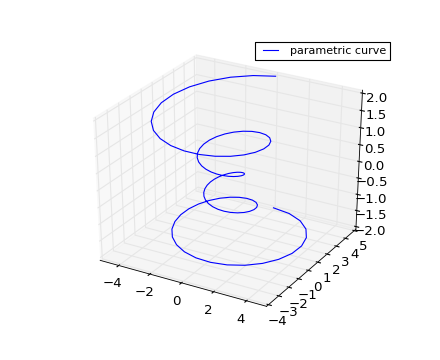
\includegraphics[scale=0.7]{images/lines3d_demo1.png}
        \caption{parametrized curve}
    \end{figure}
    By the corollary above we have
    $$Df(t)=\begin{bmatrix}
        f_1'(t)\\
        f_2'(t)\\
        f_3'(t)
    \end{bmatrix}$$
    Then the velocity vector of the curve can be represented As
    $$v(t)=f_1'(t)e_1+f_2'(t)e_2+f_3'(t)e_3$$
\end{itemize}


\begin{theorem}[Computing jacobian matrix]
    Let $f:A \subset \R^m \longrightarrow \R^n$, then 
    \begin{align}
        Df(a)=\begin{bmatrix}
            D_1f_1(a) & \cdots & D_mf_1(a)\\
            \vdots & \ddots & \vdots\\
            D_1f_n(a) & \cdots & D_mf_n(a)
        \end{bmatrix}
    \end{align}
\end{theorem}

\noindent \textbf{Example}:
\begin{itemize}
    \item Still consider the function $f:\R^2\longrightarrow \R^2$, such that 
    \begin{align}
        f(\begin{bmatrix}
               x \\
               y \\
        \end{bmatrix}) = 
        \begin{bmatrix}
            x+sin(y) \\
            y+sin(x) \\
        \end{bmatrix}
    \end{align}
    The component functions $f_1$ and $f_2$ are defined as follow:
    $$f_1:\R^2\longrightarrow\R;f_1((x,y))=x+sin(y)$$
    $$f_2:\R^2\longrightarrow\R;f_2((x,y))=y+sin(x)$$
    $f_1,f_2$ will only focus on the x-xoordinate and the y-coordinate for the vector after the transformation respectively.\\
    \begin{figure}[ht]
        \centering
        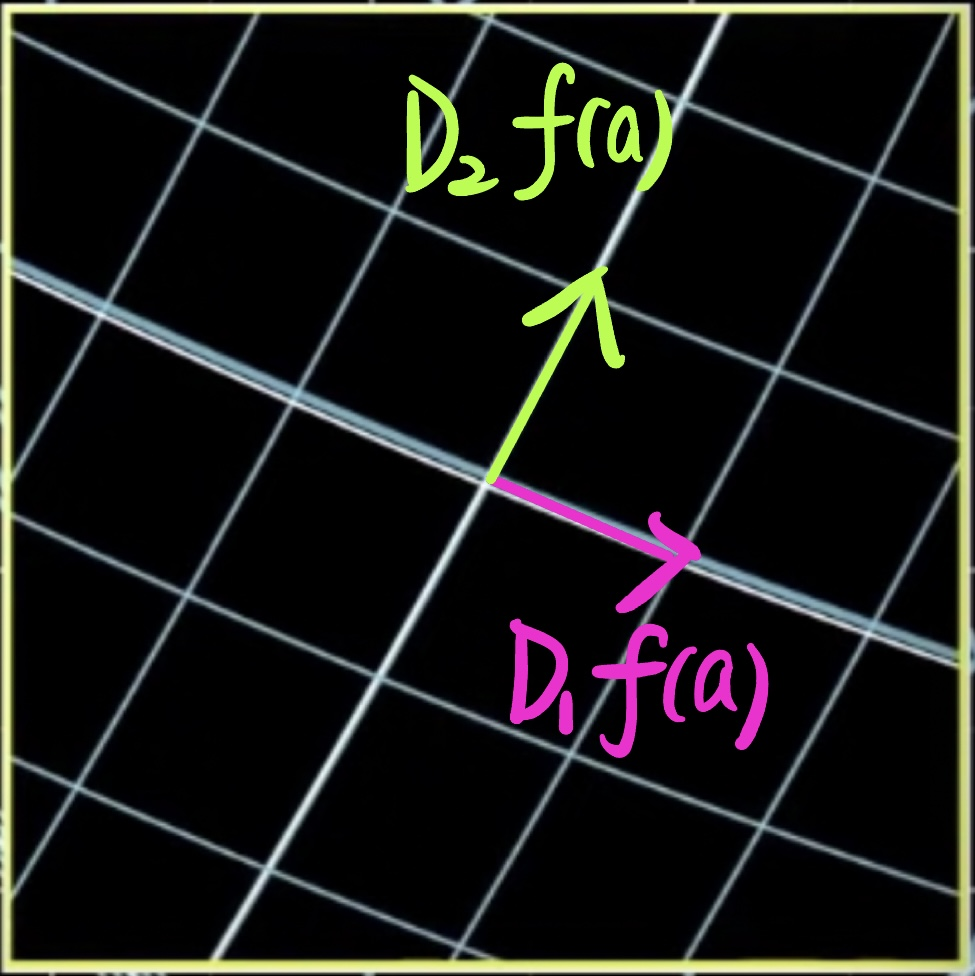
\includegraphics[scale=0.15]{images/IMG_0324.jpg}
        \caption{The place where $e_1$ and $e_2$ goes after the transformation}
    \end{figure}
    
    The matrix $B=Df(a)$ should be a 2 by 2 matrix that takes $e_1$ and $e_2$ to the corresponding spot.
    \begin{align}
        B=Df(a)=\begin{bmatrix}
            a_{1,1} & a_{1,2}\\
            a_{2,1} & a_{2,2}
        \end{bmatrix}
    \end{align}
    The vector $(a_{1,1},a_{2,1}),(a_{1,2},a_{2,2})$ is the coordinates for $D_1f(a),D_2f(a)$ respectively.\\
    If we only focus on the x-coordinates(only focus $f_1$), the first row $[a_{1,1},a_{1,2}]$ is the coordinate for $e_1,e_2$ after the transformation $f_1$.
    $$[a_{1,1},a_{1,2}]=Df_1(a)=[D_1f_1(a),D_2f_1(a)]$$
    Similarly for the second row 
    $$[a_{2,1},a_{2,2}]=Df_2(a)=[D_1f_2(a),D_2f_2(a)]$$
\end{itemize}

\section{Differentiability Classes}

\noindent \textbf{Recall}:
\begin{itemize}
    \item In single variable calculus, we can view the derivative of $f$ as a function $f':A\subset\R\longrightarrow\R$.
    It is trivial that the following statement is true.
    $$f'\text{ is continuous at }a\in A \Longrightarrow f\text{ is differentiable at } a\in A$$
    But the inverse is not true. For a very classic example
    \begin{equation}
        f(x)=
        \begin{cases}
            x^2sin(\frac{1}{x})& \text{ if }x\neq 0\\
            0& \text{ if }x=0
        \end{cases}
    \end{equation}
    \item For $f:\R\longrightarrow\R$ we defined the differentiablility classes
    \begin{itemize}
        \item $C^0$: zeroth derivative is continuous (curves are continuous).
        \item $C^1$: zeroth and first derivatives are continuous.
        \item $C^2$: zeroth, first and second derivatives are continuous.
        \item $C^k$: 0-th through k-th derivatives are continuous.
    \end{itemize}
    \item What we want is generalizing the differentiablility classes in multivariable calculus.
\end{itemize}


\begin{lemma}[Mean-Value Theorem]\label{mvt}
    If $\phi:[a,b]\longrightarrow \R$ is continuous at each point of the closed interval $[a, b]$, and differentiable at each point of the open interval $(a, b)$, then there exists a point $c \in (a, b)$ such that
    $$\phi'(c)=\frac{\phi(a)-\phi(b)}{a-b}$$
\end{lemma}


\begin{theorem} \label{continuously differentiable}
    Let $A$ be open in $\R^m$ and $f:A\subset \R^m \longrightarrow \R^n$.
    If the partial derivatives $D_jf_i(x)$ of the component functions of $f$ exist at each point $x\in A$ and are continuous on $A$.
    Then $f$ is differentiable at every $x\in A$.
\end{theorem}


\begin{definition}
    Let $A$ be open in $\R^m$ and $f:A\subset \R^m \longrightarrow \R^n$.
    \begin{itemize}
        \item $f$ is said to be \underline{of class $C^0$ on $A$}
        if $f$ is continuous on $A$.
        \item $f$ is said to be \underline{of class $C^1$ on $A$}
        if the partial derivatives $$D_jf_i(x)$$ of the component functions of $f$ exist at each point $x\in A$ and are continuous on $A$.
        \item $f$ is said to be \underline{of class $C^k$ on $A$}
        if all m-th order partial derivatives($m\leq k$) $$D_{j_1}\cdots D_{j_m}f_i$$ of the component functions of $f$ exist at each point $x\in A$ and are continuous on $A$.
        \item  $f$ is said to be \underline{of class $C^{\infty}$ on $A$} 
        if the partial derivatives of $f_i$ of all orders exist at each point $x\in A$ and are continuous on $A$
    \end{itemize}
\end{definition}
\noindent \textbf{Remark}:
\begin{itemize}
    \item Specifically, if $f$ is of class $C^1$, we say that $f$ is \underline{continuously differentiable on $A$}.
    \item We can use theorem\ref{continuously differentiable} to show that $$C^{\infty}\subset \cdots \subset C^2 \subset C^1 \subset C^0$$
\end{itemize}

\begin{theorem}
    Let $A\subset \R^m$ be open. Suppose $f:A\subset \R^m \longrightarrow\R^n$ be of class $C^2$, \\
    then $\forall i \in \{1,\cdots,n\}.\forall a \in A$ we have the relation
    $$\forall k,j \in \{1,\cdots,m\}.D_kD_jf_i(a)=D_jD_kf_i(a)$$
\end{theorem}
\noindent \textbf{Remark}:
\begin{itemize}
    \item Before trying to prove this theorem, let us get some intuition.
    Let $$f:A\subset\R^2\longrightarrow \R$$
    Consider an arbitrary $x=(a,b)\in A$, and let $h,k$ be very small.
    \begin{figure}[ht]
        \centering
        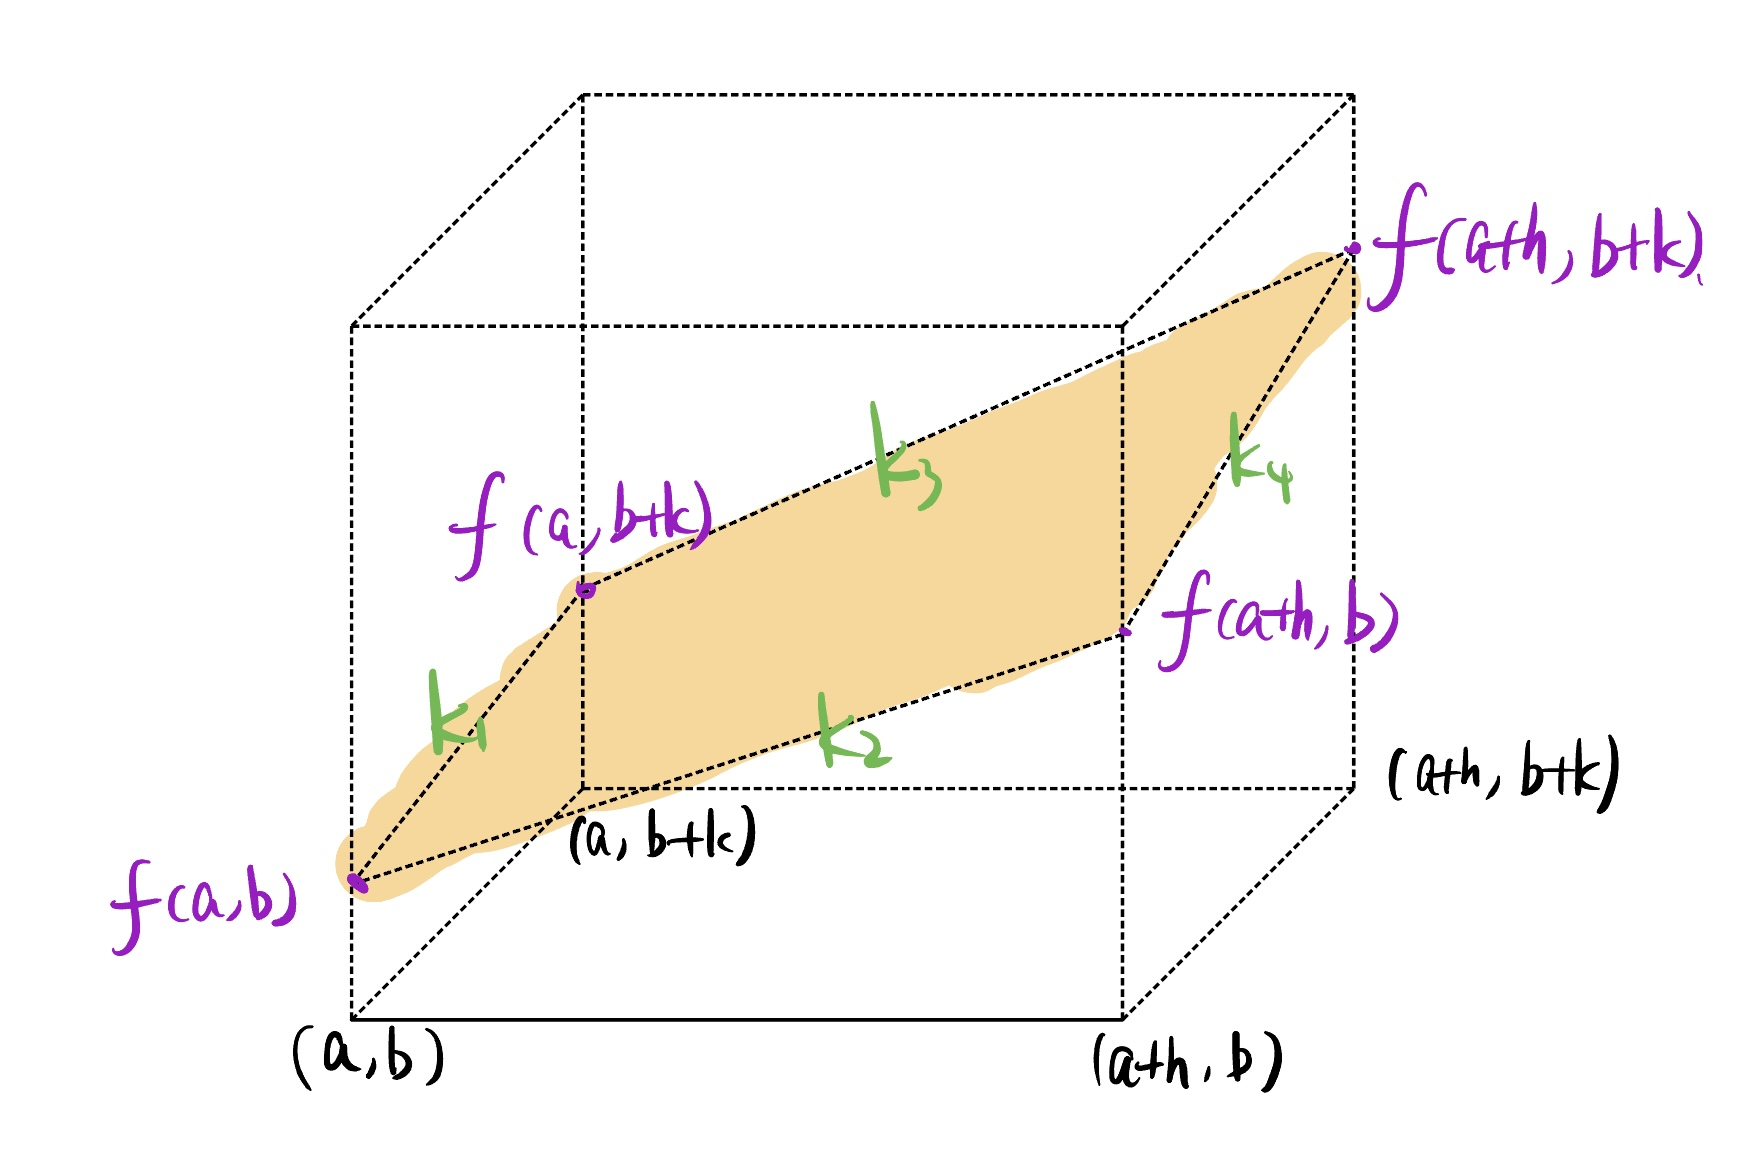
\includegraphics[scale=0.17]{images/IMG_0329.jpg}
        \caption{Geometric intuition}
    \end{figure}
    
    $Df(x)$ is the $1\times2$ matrix that represent the tangent plane at $x$.(yellow part)\\
    $D_1f(x)$ will give us the slope of the tangent line at $x$ in $e_1$ direction. For example, $$D_1f(a,b)=k_2$$
    For any point in $A\subset\R^2$, it has a corresponding slope. So 
    $$D_1f:\R^2 \longrightarrow \R$$
    By assumption, all it's partials $D_1D_1f,D_2D_1f$ are differentiable.
    \begin{equation}
        \begin{split}
            &D_2D_1f(a,b)\\
            =& \frac{k_3-k_2}{k}\\
            =& \frac{\frac{f(a+h,b+k)-f(a,b+k)}{h}-\frac{f(a+h,b)-f(a,b)}{h}}{k}\\
            =& \frac{f(a+h,b+k)-f(a,b+k)-f(a+h,b)+f(a,b)}{hk}
        \end{split}
    \end{equation}
    Similarly
    \begin{equation}
        \begin{split}
            &D_1D_2f(a,b)\\
            =& \frac{k_4-k_1}{h}\\
            =& \frac{\frac{f(a+h,b+k)-f(a+h,b)}{k}-\frac{f(a,b+k)-f(a,b)}{k}}{h}\\
            =& \frac{f(a+h,b+k)-f(a+h,b)-f(a,b+k)+f(a,b)}{hk}
        \end{split}
    \end{equation}
    So $D_2D_1f(a,b)=D_1D_2f(a,b)$. After understanding what does this theorem mean, we can formally prove it.
\end{itemize}


\begin{definition}
    Let $\vec{x}\in \R^n$, A quotient of two polynomials in multiple variables $P(\overrightarrow{x})$ and $Q(\overrightarrow{x})$
    $$R(\overrightarrow{x})=\frac{P(\overrightarrow{x})}{Q(\overrightarrow{x})}$$
    is called a \underline{rational function}, or sometimes a rational polynomial function.
\end{definition}

\begin{theorem*}\label{rational functions C_infinity}
    Let $A$ be open in $\R^m$ and let $R:A\longrightarrow \R$ be rational, then $R$ is of class $C^{\infty}$.
\end{theorem*}

\section{The Chain Rule}

\begin{definition}
    Since a matrix $A$ can be viewed as a vector, then we can define the \underline{matrix norm} of $A$, denoted as $\norm{A}$.
    satisfying the following properties:
    \begin{itemize}
        \item $\norm{A} \geq 0$ and $\norm{A}=0$ if and only if $A=0$.
        \item $\norm{\lambda A}=|\lambda|\cdot \norm{A}$ for any scaler $\lambda$.
        \item $\norm{A+B}\leq \norm{A}+\norm{B}$
    \end{itemize}
\end{definition}


\begin{definition}
    An important class of matrix norms is the \underline{subordinate matrix norms}. Given a vector norm $\norm{\cdot}$ the corresponding subordinate matrix norm is defined by
    $$\norm{A}=\sup_{x \neq 0}\frac{\norm{Ax}}{x}$$
    Or equivalently, $$\norm{A}=\sup_{\norm{x} = 1}\norm{Ax}$$
\end{definition}

\begin{lemma}\label{matrixnorm}
    A subordinate matrix norm satisfies the following properties.
    \begin{enumerate}
        \item For any vector $x$ and for any matrix $A$ $$\norm{Ax}\leq \norm{A}\cdot \norm{x}$$
        \item For ant two matrices $A$ and $B$ $$\norm{AB}\leq \norm{A}\cdot \norm{B}$$
    \end{enumerate}
\end{lemma}


\begin{definition}
    Let $A\in \mathcal{L}(\R^m,\R^n)$ be a n by m matrix. Define the \underline{ Frobenius norm}:
    $$\norm{A}_F=(\sum_{i=1}^n \sum_{j=1}^m|a_{i,j}|^2)^{\frac{1}{1}}$$
\end{definition}

\begin{theorem*}\label{all matrix norm equivalent}
    All matrix norms are equivalent.
\end{theorem*}
\noindent \textbf{Remark}:
\begin{itemize}
    \item For any $A,B\in \mathcal{L}(\R^m,\R^n)$, we define the distance function
    $$d_F(A,B)=\norm{A-B}_F$$
    This turn $\mathcal{L}(\R^m,\R^n)$ into a metric space $(\mathcal{L}(\R^m,\R^n),d_F)$.
    \item In MAT240, we proved that $\mathcal{L}(\R^m,\R^n)$ and $\R^{mn}$ are isomorphic vector spaces. It is trivial that these two metric spaces are isomorphic. $$(\mathcal{L}(\R^m,\R^n),d_F) \cong (\R^{nm},d_2)$$
    \item By theorem\ref{all matrix norm equivalent}, no matter which matrix norm we choose, it induce the same topology. So we need to take care with $(\mathcal{L}(\R^m,\R^n),d_F)$ in order to learn the structure of the topological space $\mathcal{L}(\R^m,\R^n)$.
\end{itemize}


\begin{theorem}[Chain Rule]\label{Chain Rule}
    Let $A\subset \R^m$, $B\subset \R^n$. Let $f:A\subset\R^m \longrightarrow \R^n$ and $g:B\subset\R^n \longrightarrow \R^p$ with $f(A)\subset B$.
    If $f$ is differentiable at $a$ and $g$ is differentiable at $f(a)$. Then $g \circ f$ is differentiable at $a$, furthermore $$D(g\circ f)(a)=Dg(f(a))\cdot Df(a)$$
\end{theorem}


\begin{corollary}\label{composition also in Cr}
    Let $A\subset \R^m$, $B\subset \R^n$. Let $f:A\subset\R^m \longrightarrow \R^n$ and $g:B\subset\R^n \longrightarrow \R^p$ with $f(A)\subset B$.
    If $f$ and $g$ are of class $C^r$. Then $g \circ f$ is of class $C^r$.
\end{corollary}

\begin{theorem}[MVT in multivariable]\label{MVTmultivariable}
    Let $A\subset \R^m$ be open..  Let $f:A\subset \R^m \longrightarrow \R$ be differentiable on $A$.
    If $A$ contains the line segment with end points $a$ and $b$, then there exists a point $p=a+t_0(b-a)$ in the line segment.($t_0\in(0,1)$) such that
    $$f(b)-f(a)=Df(p)(b-a)$$
\end{theorem}

\section{The Inverse Function Theorem}

\noindent \textbf{Motivation}:
\begin{itemize}
    \item Consider the system of equations 
    \begin{equation}
        \begin{cases}
            x^3-7x^2+e^x\cdot y^2+sin(y)=b_1\\
            x^4\cdot y^3-x+y=b_2
        \end{cases}
    \end{equation}
    Since it has two equations and two unknowns. 
    We can now view it as a function $f:\R^2\longrightarrow \R^2$. 
    More generaly, if we have a system of equations that has $n$ equations and $n$ unknowns, we can view it as a function $f:\R^n \longrightarrow \R^n$.
    \item Consider the easy case where $f(x)$ is linear. In other words $f(x)=Ax$ where $A$ is a fixed n by n matrix. This is now an easy linear algebra problem, if $A$ is invertible, we can find the inverse of $A$ to solve the equation. $$x=A^{-1}\cdot y_0$$
    \item Now consider a more general case, suppose $f:\R^n\longrightarrow\R^n$ is differentiable at $x_0$.  What we want is to solve $f(x)=y$ for $|y-y_0|$ very small.
    \item The non-singularity of $Df$ implies that $f$ is locally one-to-one.
\end{itemize}

\begin{theorem*}\label{TIFlemma1}
    Let $f:A \subset \R^m\longrightarrow\R^n$
    \begin{itemize}
        \item If it is differentiable, we can view its derivative as a function $$Df:\R^m\longrightarrow\mathcal{L}(\R^m,\R^n)$$
        \item If we choose the Euclidean norm $\norm{\cdot}_2$ for $\R^m,\R^n$, then we can define the matrix norm as(also works for other matrix norms) $$\norm{Df(x)}_2=\sup_{\norm{u}_2=1}\norm{Df(x)\cdot u}_2$$
    \end{itemize}
    Then we have the equivalence
    $$f\text{ is of class }C^1 \text{ on }A \Longleftrightarrow Df \text{ is continuous between metric spaces.}$$
    In other words: $f$ is of $C^1$ if and only if for any $a\in A$
    $$\forall \epsilon>0. \exists \delta>0.\forall x \in \R^m. \norm{x-a}_2<\delta \Longrightarrow \norm{Df(x)-Df(a)}_2<\epsilon$$
\end{theorem*}
\noindent \textbf{Remark}:
\begin{itemize}
    \item This is a theorem I came up with myself.
    \item This will be helpful for the next lemma for our final theorem(the inverse function theorem).
    \item If we do not specify the norm, then we just use the Euclidean norm.
    \item Theorem\ref{all matrix norm equivalent} shows that other matrix norms also work. I choose this matrix norm because we only talked about this norm in class.
    \item Actually, we can generalize this theorem further.
\end{itemize}

\begin{theorem*}\label{TIFlemma1.5}
    Let $f:A \subset \R^m\longrightarrow\R^n$
    \begin{itemize}
        \item If it is differentiable, we can view its derivative as a function $$Df:\R^m\longrightarrow\mathcal{L}(\R^m,\R^n)$$
        \item Can choose any matrix norm to turn $\mathcal{L}(\R^m.\R^n)$ into a metric space.(For convenience, we choose the Frobenius norm)
    \end{itemize}
    Then we have the equivalence for $k \geq 1$
    $$f\text{ is of class }C^k \text{ on }A \Longleftrightarrow Df \text{ is of class } C^{k-1}$$
\end{theorem*}

\begin{lemma}\label{TIFlemma2}
    Let $A$ be open in $\R^n$, let $f:A\longrightarrow\R^n$ be of class $C^1$ on $A$. 
    If $Df(a)$ is non-singular, then 
    $$\exists \epsilon>0\exists \alpha>0. \forall x_1,x_2\in B(a;\epsilon). \norm{f(x_2)-f(x_1)}\geq \alpha \norm{x_2-x_1}$$
\end{lemma}
\noindent \textbf{Remark}:
\begin{itemize}
    \item Notice that $B(a;\epsilon)\subset A$ because all $x \in B(a;\epsilon)$ is defined for $f$.
    \item This shows that $\exists \epsilon>0$ such that $f:B(a;\epsilon)\longrightarrow\R^n$ is one-to-one(injective).
    \item The term one-to-one function (injective function) must not be confused with one-to-one correspondence that refers to bijective functions
\end{itemize}

\begin{lemma}\label{extremum 0matrix}
    Let $A$ be open in $\R^n$ and $\phi:A\longrightarrow\R$. Suppose $\phi$ is differentiable on $A$ and has a local minimum(or maximum) at $x_0\in A$, then $$D\phi(x_0)=\begin{bmatrix}
        0 & \cdots & 0
    \end{bmatrix}$$
\end{lemma}


\begin{theorem}\label{TIFintermediathm}
    Let $A\subset \R^n$ be open and $f:A\longrightarrow \R^n$ be of class $C^r$ for $r \geq 1$. Let $B=f(A)$. Assume
    \begin{itemize}
        \item $f$ is one-to-one on $A$.
        \item $Df(x)$ is non-singular at all $x\in A$.
    \end{itemize}
    Then we have
    \begin{itemize}
        \item $B\in \R^n$ is open.
        \item $g=f^{-1}:B\longrightarrow A$ is also of $C^r$.
    \end{itemize}
\end{theorem}

\begin{theorem}[The Inverse Function Theorem]
    Let $A$ be open in $\R^n$ and let $f:A\longrightarrow \R^n$ be of class $C^r$. 
    If $Df$ is non-singular at the point $a\in A$.
    Then we have
    \begin{itemize}
        \item There is an open $U$ containing $a$ and an open $V\subset\R^n$ containing $f(a)$ such that $f:U\longrightarrow V$ is bijective.
        \item The inverse $g=f^{-1}:V \longrightarrow U$ is also of class $C^r$.
    \end{itemize}
\end{theorem}

\noindent \textbf{Remark}:
\begin{itemize}
    \item This is a very long and difficult theorem, but it is very important.
    \item In the future, we will generalize this theorem in terms of differentiable maps between differentiable manifolds.$$F:M\longrightarrow N$$ 
    \item If the derivative is non-singular at a point $a$, then we have a very nice result. There is a small part $U$ of $M$ containing $a$ and a small part $V$ of $N$ containing $F(a)$, such that $U$ and $V$ are isomorphic.
\end{itemize}

\section{Applications}

\subsection{Approximation}

There are four kinds of multivariable functions
\begin{itemize}
    \item Curves: $f:\R\longrightarrow \R^n$
    \item Surfaces: $f:\R^2\longrightarrow \R^n$
    \item Scaler fields: $f:\R^n \longrightarrow \R$
    \item Vector fields: $f:\R^n \longrightarrow \R^m$
\end{itemize}
In this section, we will focus on the scalar fields. For example
\begin{itemize}
    \item In physics, we often encounter fields, which is a function associating a single number to every point in a space.
    \item In machine learning and artificial intelligence, we have the cost function(sometimes also called an error function) which is a function that maps an event or values of one or more variables onto a real number intuitively representing some cost associated with the event.
\end{itemize}
Our goal is to learn the optimization for scalar field functions.\\
\begin{definition}
    We say a function $f(x_1,\cdots,x_n)$ is \underline{linear} if $$f(x_1,\cdots,x_n)=a_1x_1+\cdots+a_nx_n+c$$
\end{definition}

\begin{definition}
    A \underline{linear form} is a polynomial with terms all of degree one.
\end{definition}

\begin{definition}
    Given a differentiable function $f:\R^n\longrightarrow \R$ and a point $a\in \R^n$. The \underline{linear approximation} of $f$ at $a$ is
    $$L(x)=f(a)+Df(a)\cdot (x-a)$$
\end{definition}
\noindent \textbf{Remark}:
\begin{itemize}
    \item Let $x=(x_1,\cdots,x_n)$ and $a=(a_1,\cdots,a_n)$. Then 
    \begin{equation}
        \begin{split}
            L(x_1,\cdots,x_n)&=f(a)+Df(a)\cdot (x-a)\\
            &= f(a)+ \begin{bmatrix}
                D_1f(a) & \cdots & D_nf(a)
            \end{bmatrix}\cdot \begin{bmatrix}
                x_1-a_1\\
                \vdots\\
                x_n-a_n
            \end{bmatrix}\\
            &= f(a)+ D_1f(a)(x_1-a_1)+\cdots+D_nf(a)(x_n-a_n)\\
            &= f(a)+ \nabla f(a)\cdot (x_1-a_1,\cdots,x_n-a_n)
        \end{split}
    \end{equation}
\end{itemize}

\begin{definition}
    We say a function $f(x_1,\cdots,x_n)$ is \underline{quadratic} if $f$ is a polynomial of degree 2.
\end{definition}
\noindent \textbf{Example}:
\begin{itemize}
    \item $f(x)=ax^2+bx+c$ is a quadratic function of one variable.
    \item $f(x,y)=ax^2+by^2+cxy+dx+ey+f$ is a quadratic function of two variables.
    \item $f(x,y,z)=ax^2by^2+cz^2+dxy+exz+fyz+gx+hy+iz+j$ is a quadratic function of three variables.
\end{itemize}

\begin{definition}
    A \underline{quadratic form} is a polynomial with terms all of degree two.
\end{definition}
\noindent \textbf{example}:
\begin{itemize}
    \item $ax^2+2bxy+cy^2$ is a quadratic form. Also notice that
    \begin{equation}
        ax^2+2bxy+cy^2=\begin{bmatrix}
            x & y
        \end{bmatrix}\begin{bmatrix}
            a & b\\
            b & c
        \end{bmatrix}\begin{bmatrix}
            x\\
            y
        \end{bmatrix}
    \end{equation}
    \item $ax^2+dy^2+fz^2+2bxy+2cxz+2dyz$ is a quadratic form. Also notice that
    \begin{equation}
        ax^2+dy^2+fz^2+2bxy+2cxz+2dyz=\begin{bmatrix}
            x & y & z
        \end{bmatrix}\begin{bmatrix}
            a & b & c\\
            b & d & e\\
            c & e & f
        \end{bmatrix}\begin{bmatrix}
            x\\
            y\\
            z
        \end{bmatrix}
    \end{equation}
\end{itemize}
\noindent \textbf{Remark}:
\begin{itemize}
    \item A quadratic function $f(x_1,\cdots,x_n)$ can be witten as a sum of a linear form $l(x_1,\cdots,x_n)$ and a quadratic form $q(x_1,\cdots,x_n)$ plus a constant.
    $$f(x_1,\cdots,x_n)=c+l(x_1,\cdots,x_n)+q(x_1,\cdots,x_n)$$
    \item As $n$ getting more and more large, the quadratic form $q(x_1,\cdots,x_n)$ will getting extremly complicated. It is our desire to use an associated matrix to get the quadratic form.
\end{itemize}

\begin{definition}
    Let $f:\R^n\longrightarrow \R$ be of class $C^2$. The \underline{Hessian matrix} of $f$ at point $a$ is defined as
    $$Hf(a)=\begin{bmatrix}
        D_1D_1f(a) & \cdots & D_1D_nf(a)\\
        \vdots & \ddots & \vdots\\
        D_nD_1f(a) & \cdots & D_nD_nf(a)
    \end{bmatrix}$$
    sometimes we also use the notation $D^2f(a)$ to denote the Hessian matrix.
\end{definition}
\noindent \textbf{Remark}:
\begin{itemize}
    \item The Hessian matrix of a function $f$ at point $a$ contains all the information of all second order partial derivatives of $f$ at $a$.
    \item Consider the gradient of $f$
    $$\nabla f :\R^n \longrightarrow\R^n$$
    The Hessian matrix of $f$ is the Jacobian matrix of the gradient of $f$.
    $$Hf=D(\nabla f)$$
    \item The Hessian matrix of $f$ can also be viewed as the Jacobian matrix of the Jacobian matrix of $f$.
    $$Hf=D(D f)$$
    This is why we choose the notation $D^2f$.
\end{itemize}

\begin{definition}
    Let $f:\R^n\longrightarrow \R$ be of class $C^2$. Then the \underline{quadratic approximation} of $f$ at the point $a$ is 
    $$Q(x)=f(a)+Df(a)\cdot(x-a)+\frac{1}{2}(x-a)^TD^2f(a)(x-a)$$
\end{definition}
\noindent \textbf{Remark}:
\begin{itemize}
    \item Let $x=(x_1,\cdots,x_n)$ and $a=(a_1,\cdots,a_n)$. $(x-a)^T$ denote the transpose of the vector $(x-a)$.
    $$(x-a)^T=\begin{bmatrix}
        x_1-a_1\\
        \vdots\\
        x_n-a_n
    \end{bmatrix}^T=\begin{bmatrix}
        x_1-a_1 & \cdots & x_n-a_n
    \end{bmatrix}$$
    \item Can check that
    \begin{itemize}
        \item $Q(a)=f(a)$
        \item $D_iQ(a)=D_if(a)$ for all $i$.
        \item $D_iD_jQ(a)=D_iD_jf(a)$ for all $i,j$.
        \item All partial derivatives of order geater than or equal to three are all zero.
    \end{itemize}
    \item The quadratic approximation will be very useful in physics.
\end{itemize}
\noindent \textbf{Example}:
\begin{itemize}
    \item Let $f:\R^2 \longrightarrow \R$ be of class $C^2$. The quadratic approximation for $f$ at point $a=(a_1,a_2)$ is
    \begin{equation}
        \begin{split}
            Q(x_1,x_2)=&f(a)+D_1f(a)(x_1-a_1)+D_2f(a)(x_2-a_2)\\
            &+\frac{1}{2}D_1D_1f(a)(x_1-a_1)^2+D_1D_2f(a)(x_1-a_1)(x_2-a_2)+\frac{1}{2}D_2D_2f(a)(x_2-a_1)^2
        \end{split}
    \end{equation}
    \item Let $f(x,y)=e^{\frac{x}{2}}sin(y)$. Compute the quadratic approximation of $f$ at $(0,\frac{\pi}{2})$
    $$f(0,\frac{\pi}{2})=e^0sin(\frac{\pi}{2})=1$$
    $$D_1f(x,y)=\frac{1}{2}e^{\frac{\pi}{2}}sin(y);\quad D_1f(0,\frac{\pi}{2})=\frac{1}{2}$$
    $$D_2f(x,y)=e^{\frac{\pi}{2}}cos(y);\quad D_2f(0,\frac{\pi}{2})=0$$
    $$D_1D_1f(x,y)=\frac{1}{4}e^{\frac{\pi}{2}}cos(y);\quad D_1D_1f(0,\frac{\pi}{2})=\frac{1}{4}$$
    $$D_2D_2f(x,y)=-e^{\frac{\pi}{2}}sin(y);\quad D_2D_2f(0,\frac{\pi}{2})=-1$$
    The linear approximation of $f$ at $a$ is 
    \begin{equation}
        \begin{split}
            L(x,y)&=f(0,\frac{\pi}{2})+D_1f(0.\frac{\pi}{2})(x-0)+D_2f(0,\frac{\pi}{2})(y-\frac{\pi}{2})\\
            &=1 + \frac{1}{2}x+0\\
            &= \frac{1}{2}x+1
        \end{split}
    \end{equation}
    So the quadratic approximation is 
    \begin{equation}
        \begin{split}
            Q(x,y)&=L(x,y)+\frac{1}{2}D_1D_1f(0,\frac{\pi}{2})(x-0)^2+D_1D_2f(0,\frac{\pi}{2})(x-0)(y-\frac{\pi}{2})+\frac{1}{2}D_2D_2f(0,\frac{\pi}{2})(y-\frac{\pi}{2})^2\\
            &= L(x,y)+\frac{1}{2}x^2-\frac{1}{2}(y-\frac{\pi}{2})^2\\
            &= 1+\frac{1}{2}x+\frac{1}{2}x^2-\frac{1}{2}(y-\frac{\pi}{2})^2
        \end{split}
    \end{equation}
\end{itemize}

\subsection{Optimization(with constraints)}

\begin{definition}
    Let $f:A\subset \R^n \longrightarrow \R$ 
    \begin{enumerate}
        \item $f$ is said to have a \underline{local maxima} at the point $a\in A$ if 
        $$\exists \delta>0.\forall x \in A. \norm{x-a}<\delta\Longrightarrow f(x)\leq f(a)$$
        \item $f$ is said to have a \underline{local minima} at the point $a\in A$ if 
        $$\exists \delta>0.\forall x \in A. \norm{x-a}<\delta\Longrightarrow f(x)\geq f(a)$$
    \end{enumerate}
\end{definition}
\noindent \textbf{Remark}:
\begin{itemize}
    \item One of our goals is to find the local extrema of the function $f$.
    \item It is trivial that if $f$ has a local extrema at the point $a$, then
    $$D_1f(a)=\cdots =D_nf(a)=0$$
    But the converse may not be true. For example
    \begin{itemize}
        \item The function $f(x)=x^3$ has derivative $f'(0)=0$, but the point $x=0$ is not an extrema.
        \item The function $f(x,y)=x^2-y^2$ has $Df(0,0)=[0,0]$, but $(0,0)$ is not an extrema.
        \begin{figure}[H]
            \centering
            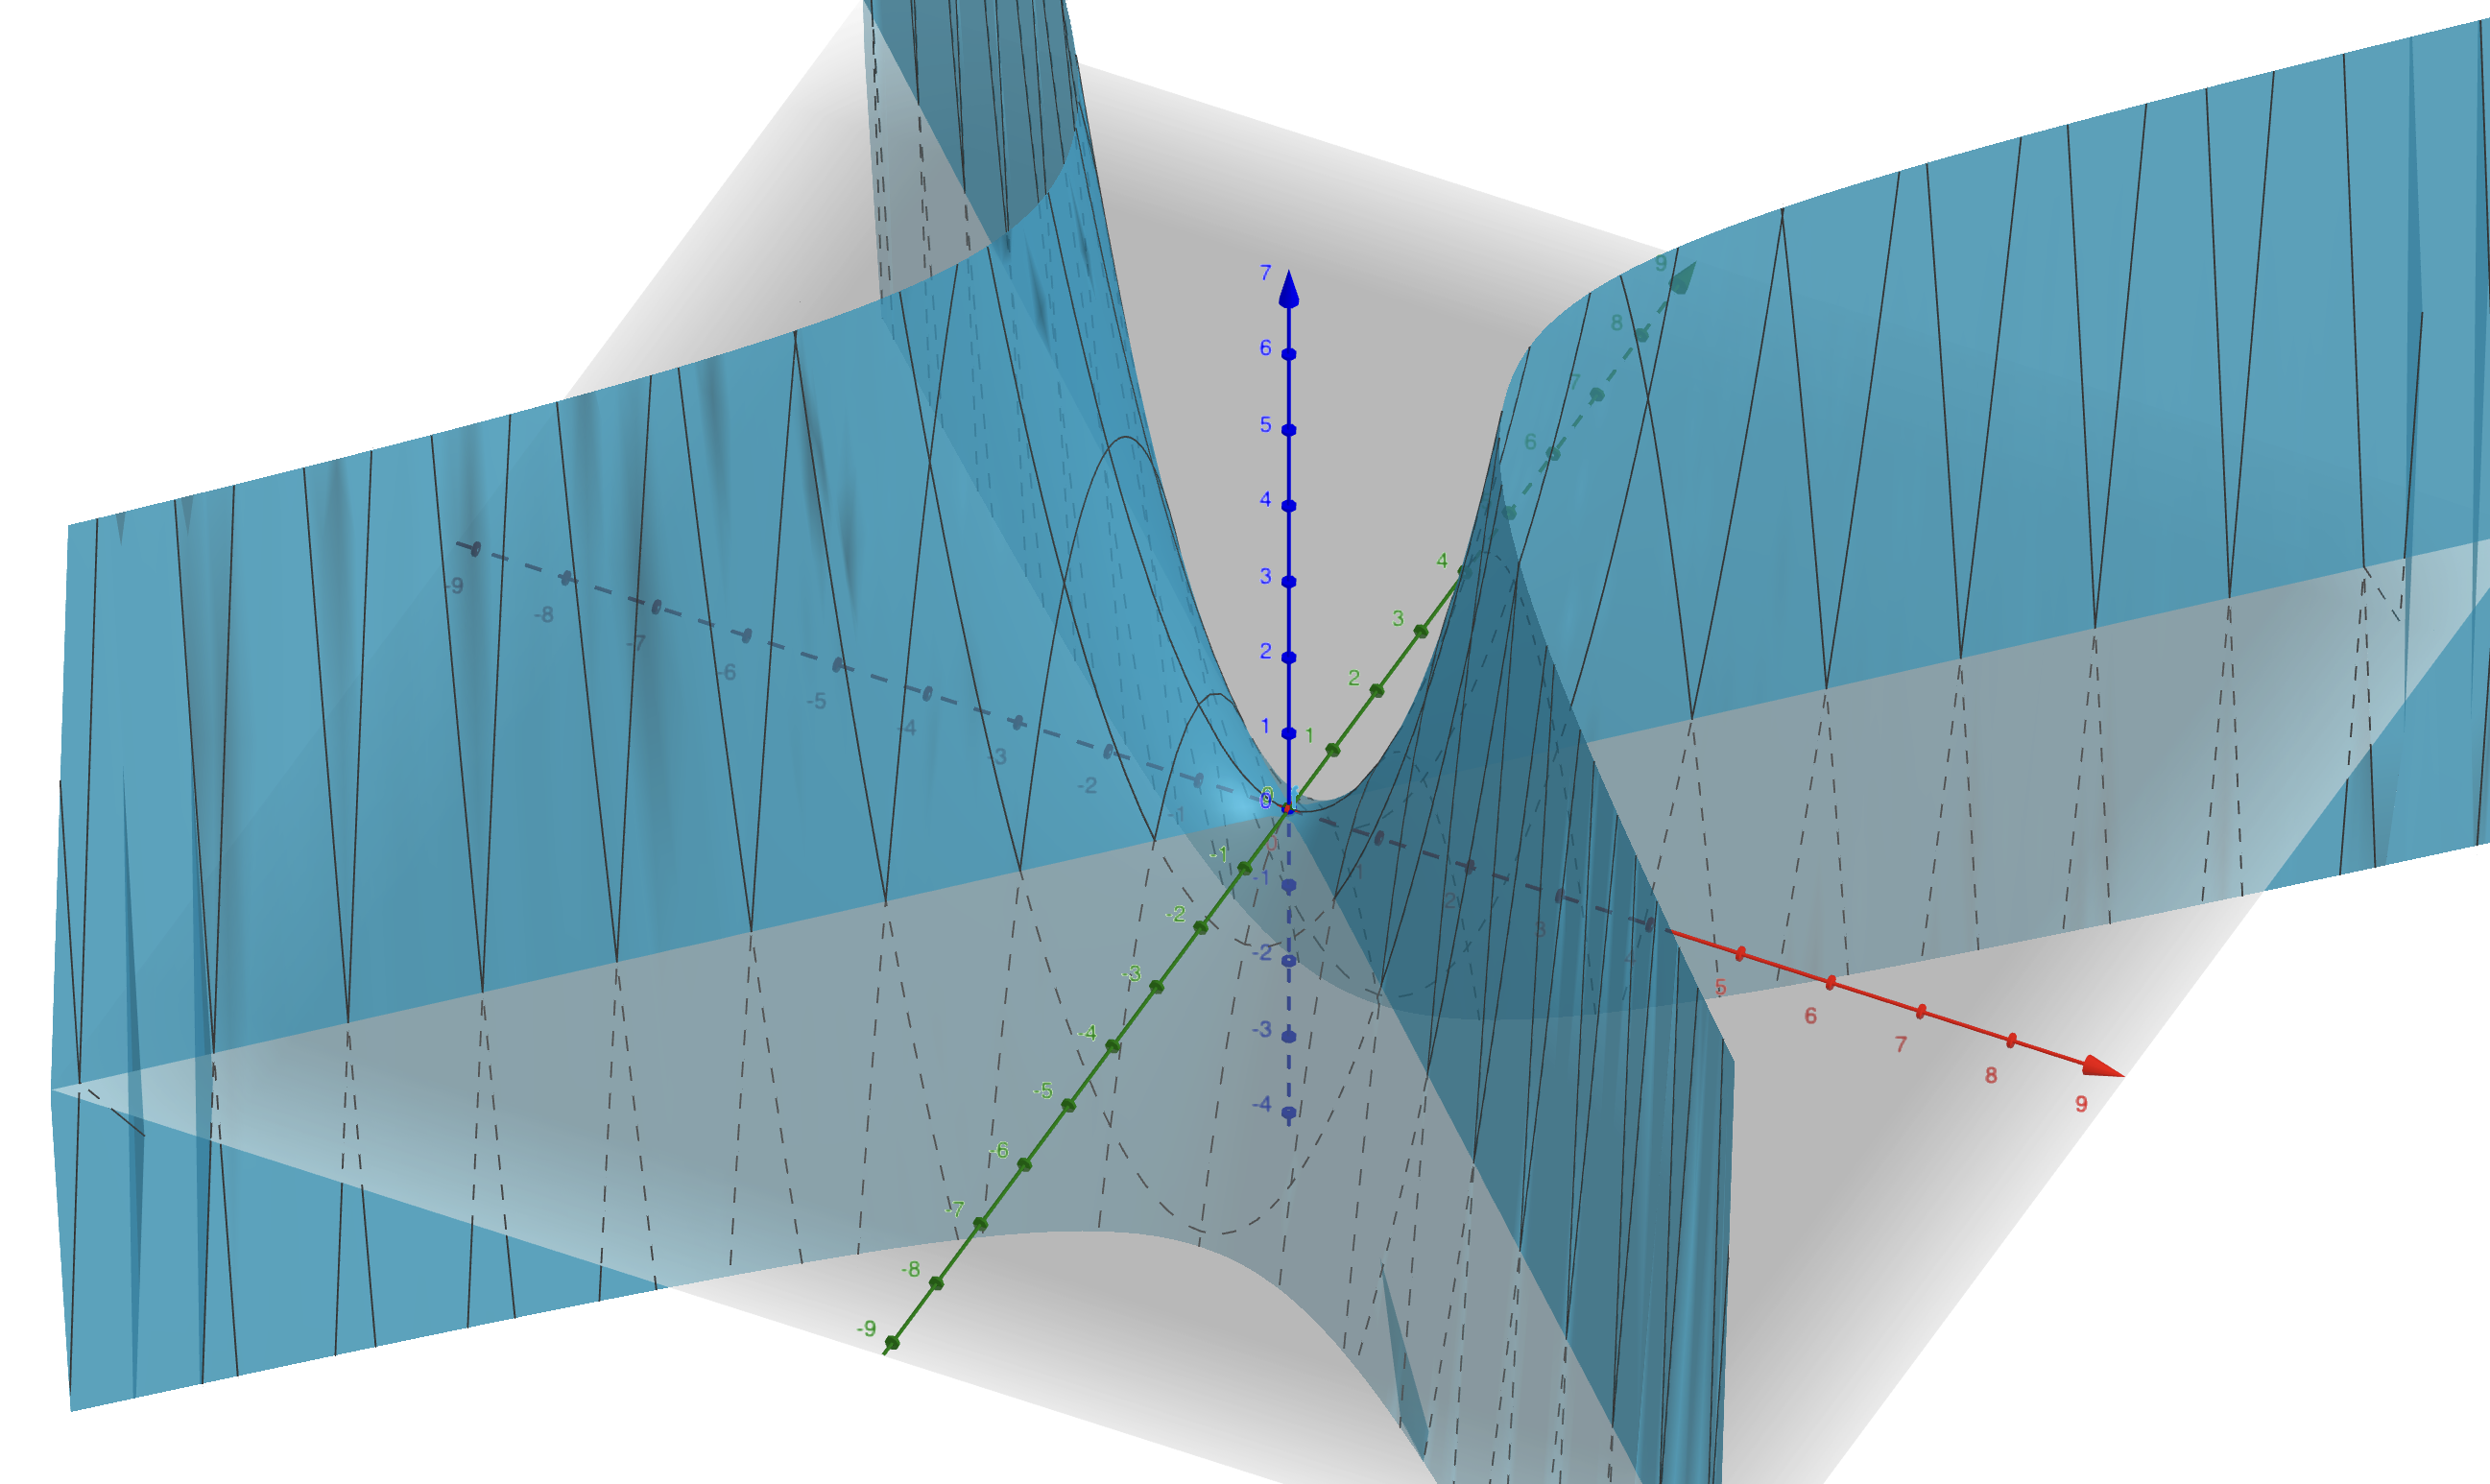
\includegraphics[scale=0.2]{images/Screen Shot 2022-10-26 at 02.39.56.png}
            \caption{$f(x,y)=x^2-y^2$}
        \end{figure}
    \end{itemize}
\end{itemize}

\begin{definition}
    Let $f:\R^2\longrightarrow \R$. A point $a$ is called a \underline{saddle point} if all partial derivatives $D_if(a)=0$ but $a$ is neither a maxima nor a minima.
\end{definition}

\begin{theorem*}[The Second Partial Derivative Test For Two variables]
    Let $f:\R^2\longrightarrow \R$ be of class $C^2$. Let 
    $$h=D_1D_1f(x)\cdot D_2D_2f(x)-(D_1D_2f(x))^2$$
    If $\nabla f(x)=\vec{0}$, then
    \begin{enumerate}
        \item If $h>0$ and $D_1D_1f(x)>0$, then  $x$ is a minima.
        \item If $h>0$ and $D_1D_1f(x)<0$, then  $x$ is a maxima.
        \item If $h<0$, then $x$ is a saddel point.
    \end{enumerate}
\end{theorem*}
\noindent \textbf{Example}:
\begin{itemize}
    \item Find all maxima and minima for $$f(x,y)=3x^2y-y^3-3x^2-3y^2$$
    First, solve the equation $$\nabla f(x)=\begin{bmatrix}
        D_1f(x,y)\\
        D_2f(x,y)
    \end{bmatrix}=\begin{bmatrix}
        6xy-6x\\
        3x^2-3y^2-6y
    \end{bmatrix}=\begin{bmatrix}
        0\\
        0
    \end{bmatrix}$$
    We get four points: $(0,0)$, $(0,-2)$, $(\sqrt{3},1)$, $(-\sqrt{3},1)$.
    $$D_1D_1f(x,y)=6y-6$$
    $$D_2D_1f(x,y)=6x$$
    $$D_2D_2f(x,y)=-6y-6$$
    \begin{figure}[H]
        \centering
        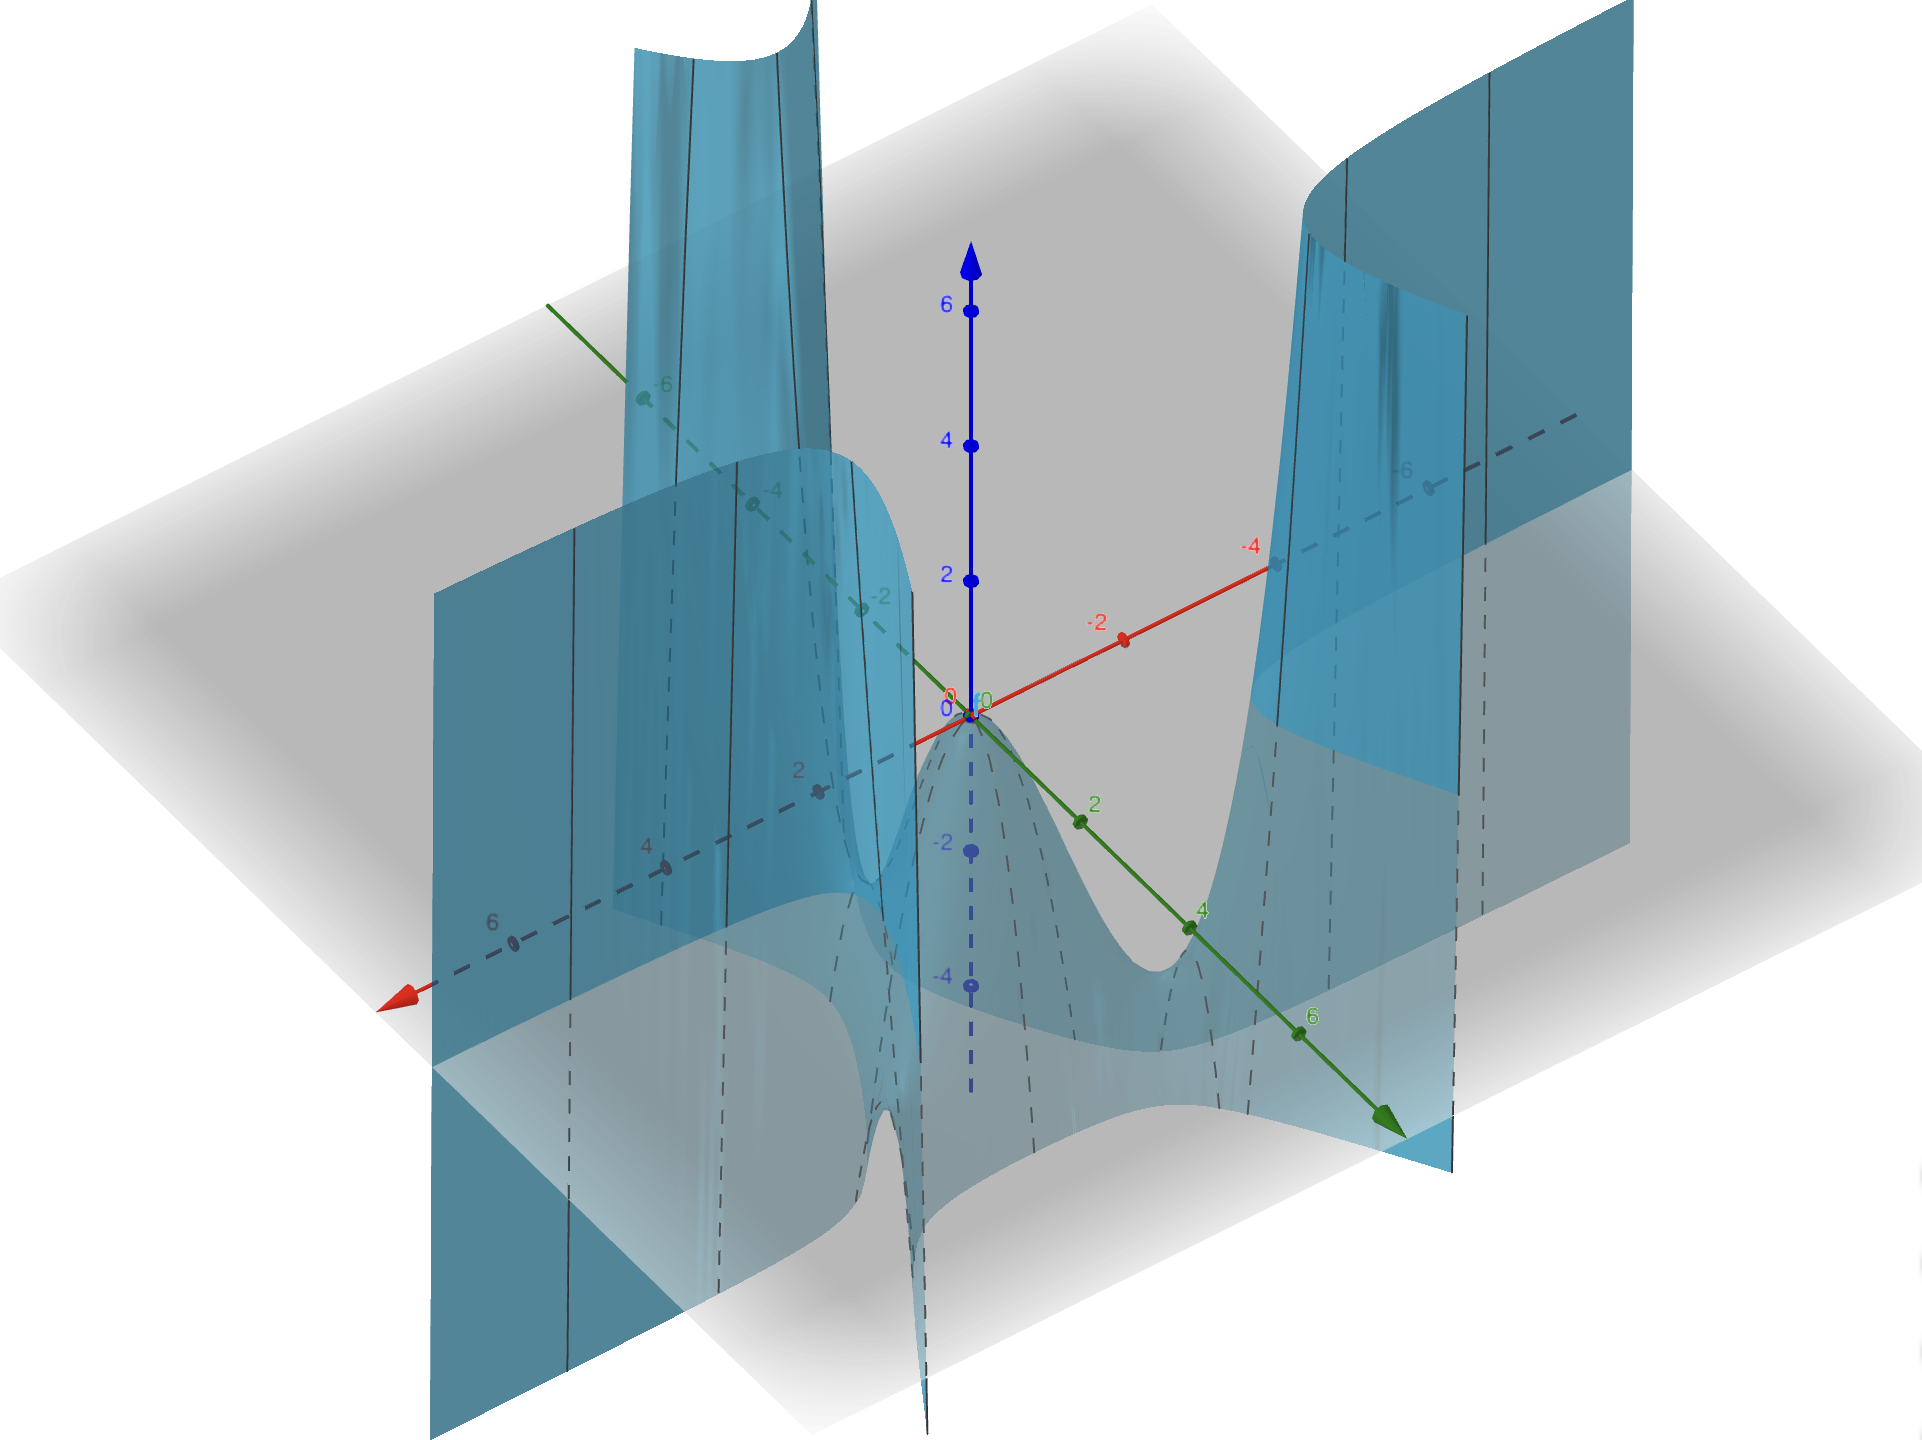
\includegraphics[scale=0.21]{images/Screen Shot 2022-10-26 at 03.53.45.png}
        \caption{$f(x,y)=3x^2y-y^3-3x^2-3y^2$}
    \end{figure}
    \begin{itemize}
        \item $(0,0)$: $h=(-6)(-6)-0^2>0 \Longrightarrow (0,0)$ is a maxima.
        \item $(0,-2)$: $h=(-18)(6)-0^2<0 \Longrightarrow (0,-2)$ is a saddle point.
        \item $(\sqrt{3},1)$: $h=0(-6)-108<0 \Longrightarrow (\sqrt{3},1)$ is a saddle point.
        \item $(-\sqrt{3},1)$: $h=0(-6)-108<0 \Longrightarrow (-\sqrt{3},1)$ is a saddle point.
    \end{itemize}
\end{itemize}
\noindent \textbf{Remark}:
\begin{itemize}
    \item In this case, $h=det(Hf)$.
    \item In order to generalize this criterion to $n$ variables, we need the following definitions.
\end{itemize}

\begin{definition}
    Let $A$ be a n by n matrix. We say $A$ is \underline{symmetric} if and only if $$A=A^T$$
\end{definition}
\noindent \textbf{Remark}:
\begin{itemize}
    \item The Hessian matrix $Hf$ is always symmetric.
\end{itemize}

\begin{definition}
    Let $A$ be a n by n symmetric matrix with real entries.
    \begin{enumerate}
        \item We say $A$ is \underline{positive-defined} if for all $x\in \R^n$
        $$x^TAx>0$$
        \item We say $A$ is \underline{negative-defined} if for all $x\in \R^n$
        $$x^TAx<0$$
        \item We say $A$ is \underline{indefined} if for all $x\in \R^n$
        $$x^TAx=0$$
    \end{enumerate}
\end{definition}

\begin{theorem*}
    Let $A=(a_{i,j})$ be a n by n symmetric matrix with real entries.
    \begin{enumerate}
        \item $A$ is positive-defined if and only if
        $$a_{1,1}>0, \quad \begin{vmatrix}
            a_{1,1} & a_{1,2}\\
            a_{2,1} & a_{2,2}
        \end{vmatrix}>0, \quad \begin{vmatrix}
            a_{1,1} & a_{1,2} & a_{1,3}\\
            a_{2,1} & a_{2,2} & a_{2,3}\\
            a_{3,1} & a_{3,2} & a_{3,3}
        \end{vmatrix}>0, \quad \cdots \quad det(A)>0$$
        \item $A$ is negative-defined if and only if
        $$a_{1,1}<0, \quad \begin{vmatrix}
            a_{1,1} & a_{1,2}\\
            a_{2,1} & a_{2,2}
        \end{vmatrix}>0, \quad \begin{vmatrix}
            a_{1,1} & a_{1,2} & a_{1,3}\\
            a_{2,1} & a_{2,2} & a_{2,3}\\
            a_{3,1} & a_{3,2} & a_{3,3}
        \end{vmatrix}<0, \quad \begin{vmatrix}
            a_{1,1} & a_{1,2} & a_{1,3} & a_{1,4}\\
            a_{2,1} & a_{2,2} & a_{2,3} & a_{2,4}\\
            a_{3,1} & a_{3,2} & a_{3,3} & a_{3,4}\\
            a_{4,1} & a_{4,2} & a_{4,3} & a_{4,4}
        \end{vmatrix}>0\cdots$$
    \end{enumerate}
\end{theorem*}

\begin{theorem*}[The Second Partial Derivative Test]
    Let $f:\R^n\longrightarrow \R$ be of class $C^2$.\\
    If $\nabla f(x)=\vec{0}$, then
    \begin{enumerate}
        \item If $Hf(x)$ is positive-defined, then  $x$ is a minima.
        \item If $Hf(x)$ is negative-defined, then  $x$ is a maxima.
        \item If $Hf(x)$ is indefined, then $x$ is not an extrema.
    \end{enumerate}
\end{theorem*}

\begin{definition}
    A \underline{contour line} (also isoline, isopleth, or isarithm) of a function of two variables is a curve along which the function has a constant value, so that the curve joins points of equal value.
\end{definition}
\noindent \textbf{Remark}:
\begin{itemize}
    \item The gradient of the function is always perpendicular to the contour lines.
    \begin{figure}[H]
        \centering
        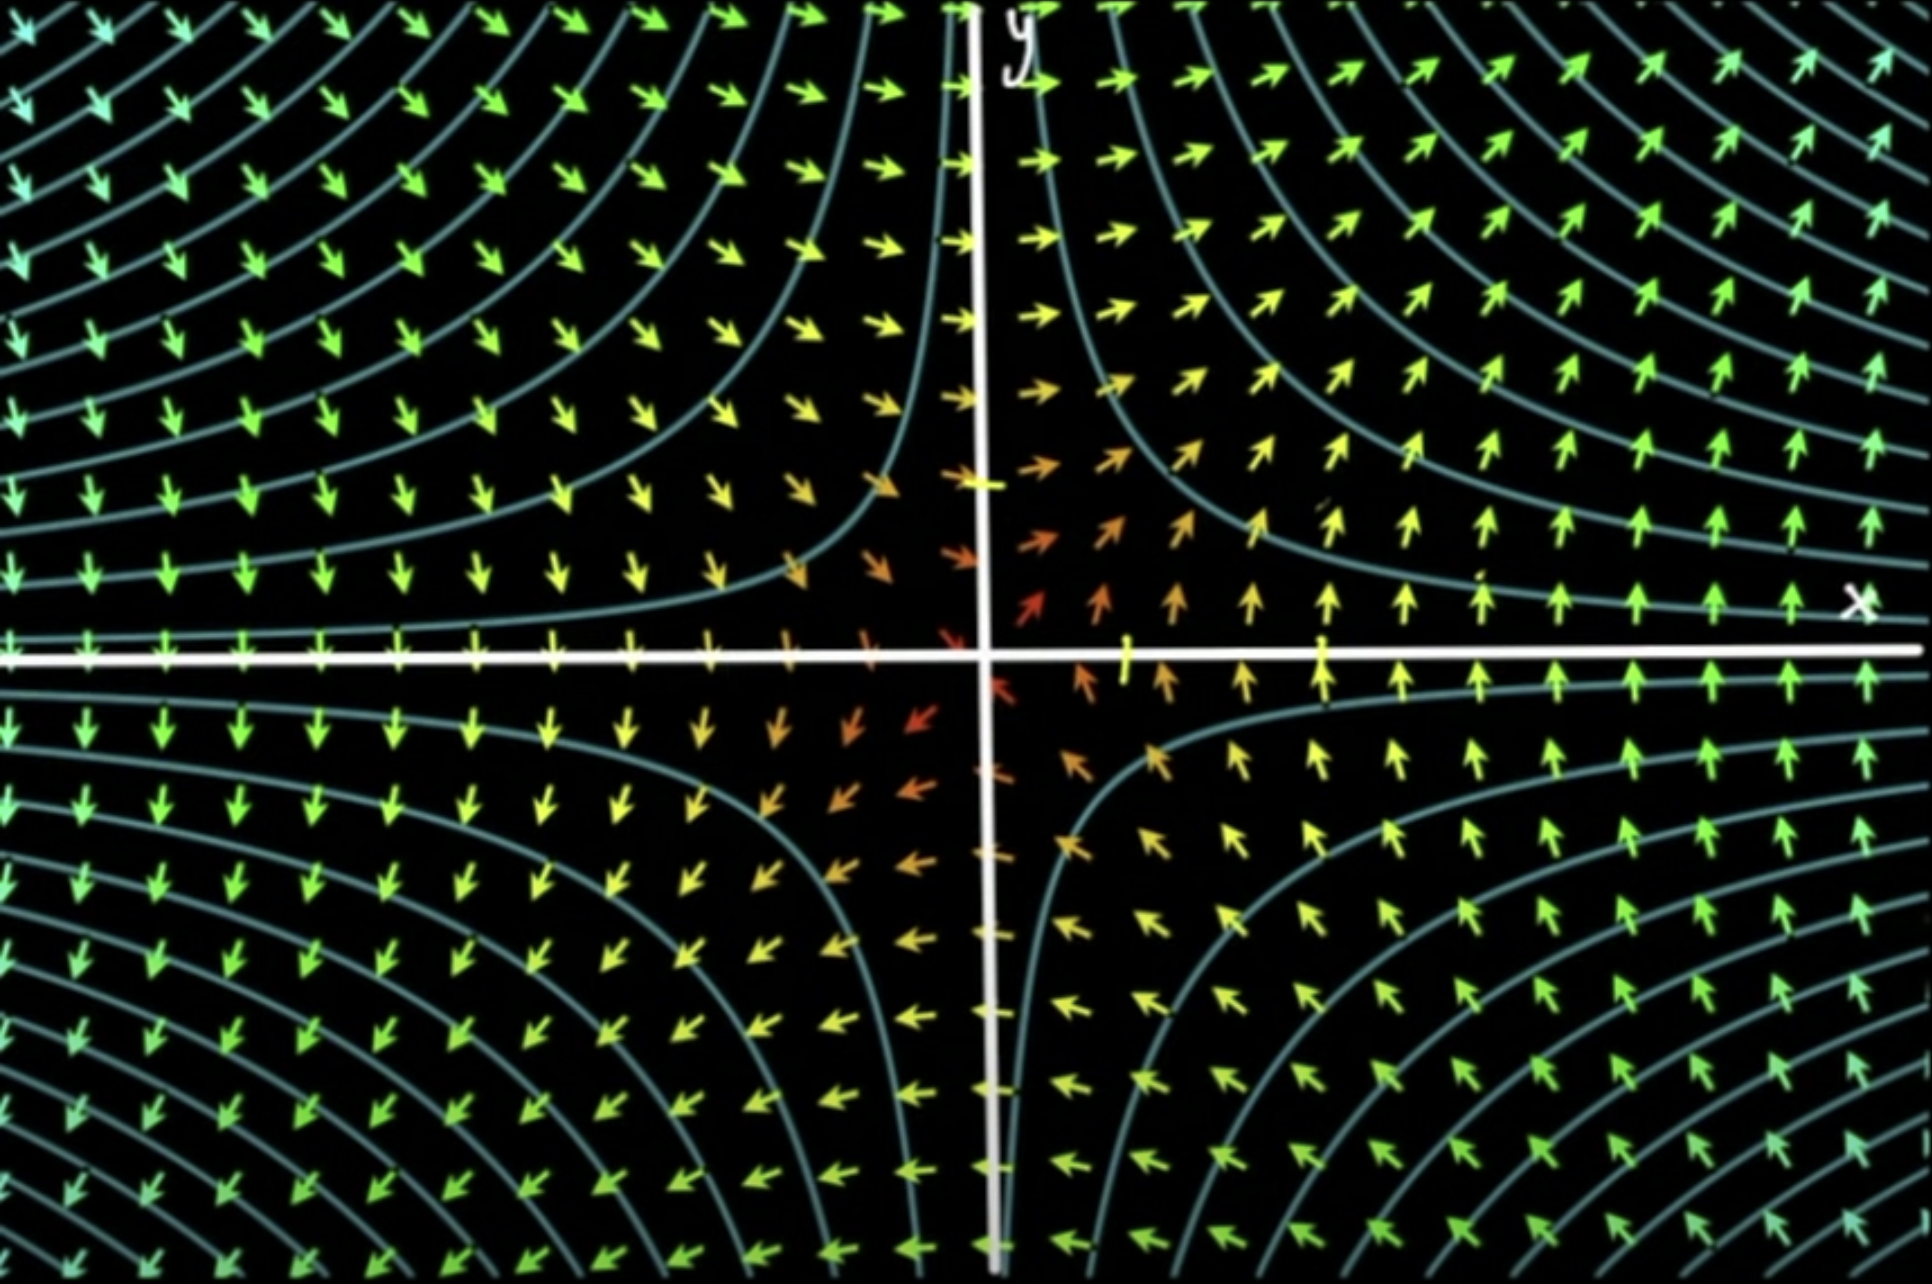
\includegraphics[scale=0.3]{images/Screen Shot 2022-10-26 at 13.04.34.png}
        \caption{Contour lines and gradient for $f(x,y)=xy$}
    \end{figure}
    \item When the lines are close together the magnitude of the gradient is large: the variation is steep.
    \item The idea of contour lines is very useful in real world applications like physics, geology,social science.
\end{itemize}

\begin{theorem}[Lagrange Multiplier]
    Given a function $f:A\subset \R^n\longrightarrow \R$, and constrains
    $$g_1(x_1,\cdots,x_n)=0,\cdots ,g_k(x_1,\cdots,x_n)=0$$
    We can solve the system of equations to get all critical points.
    \begin{equation}
        \begin{cases}
            \nabla f(x)=\sum_{i=1}^k \lambda_i \nabla g_i(x)\\
            g_1(x)=\cdots=g_k(x)=0
        \end{cases}
    \end{equation}
\end{theorem}
\noindent \textbf{Example}:
\begin{itemize}
    \item Find the maximum of $f(x,y)=x^2y$ given the constrain $g(x,y)=x^2+y^2-1=0$.\\
    \begin{figure}[H]
        \centering
        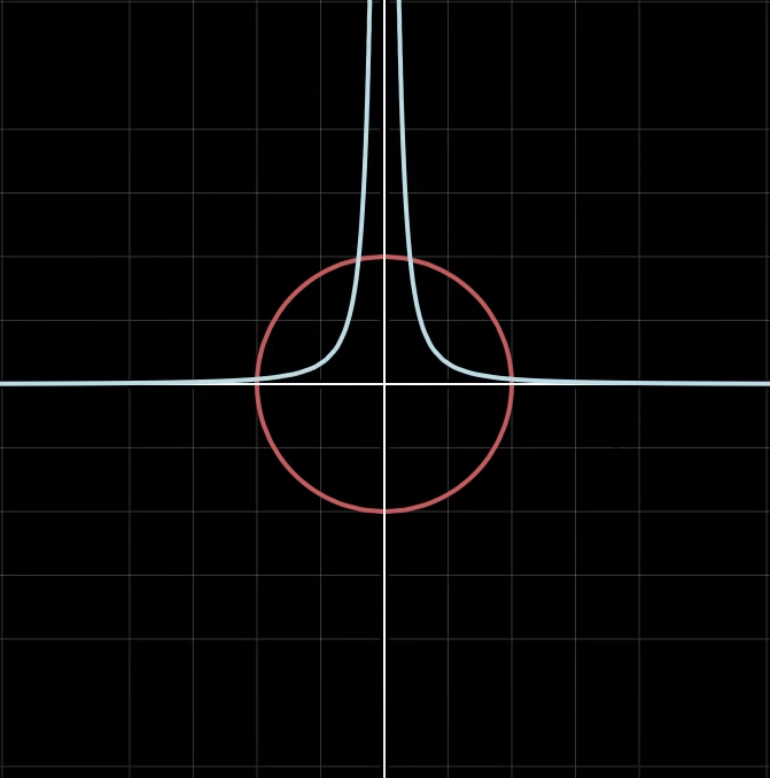
\includegraphics[scale=0.4]{images/Screen Shot 2022-10-26 at 14.31.58.png}
        \caption{One of the contour lines of $f$ and $g$.}
    \end{figure}
    
    As shown in the picture, the red circle represent the contour line of $g$ for $g(x)=0$. Our goal is to find the contour line of $f$ which is tangent to this red circle.
    We already know that the gradient is always perpendicular to the contour line. So the equation $$\nabla f(x)=\lambda \nabla g(x)$$
    gives us all the cases that one of the contour line of $f$ is tangent to one of the contour line of $g$. The equation $$g(x)=0$$
    constrain the contour line of $g$ to this red circle. So solving the system of equations 
    \begin{equation}
        \begin{cases}
            \nabla f(x)=\lambda \nabla g(x)\\
            g(x)=0
        \end{cases}
    \end{equation}
    will give us all the critical points. further, if we check all the value of these pointss, we can get the maximum and he minimum we want.
    $$\nabla f =\begin{bmatrix}
        D_1f\\
        D_2f
    \end{bmatrix}=\begin{bmatrix}
        2xy\\
        x^2
    \end{bmatrix}$$
    $$\nabla g =\begin{bmatrix}
        D_1g\\
        D_2g
    \end{bmatrix}=\begin{bmatrix}
        2x\\
        2y
    \end{bmatrix}$$
    Therefore, we need to solve 
    \begin{equation}
        \begin{cases}
            2xy=\lambda \cdot 2x\\
            x^2=\lambda\cdot 2y\\
            x^2+y^2=1
        \end{cases}
    \end{equation}
    We get four points: $(\sqrt{\frac{2}{3}},\sqrt{\frac{1}{3}})$, $(-\sqrt{\frac{2}{3}},\sqrt{\frac{1}{3}})$, $(\sqrt{\frac{2}{3}},-\sqrt{\frac{1}{3}})$, $(-\sqrt{\frac{2}{3}},-\sqrt{\frac{1}{3}})$\\
    Can check that the first point and the second point are both the maximum we want.
    \begin{figure}[H]
        \centering
        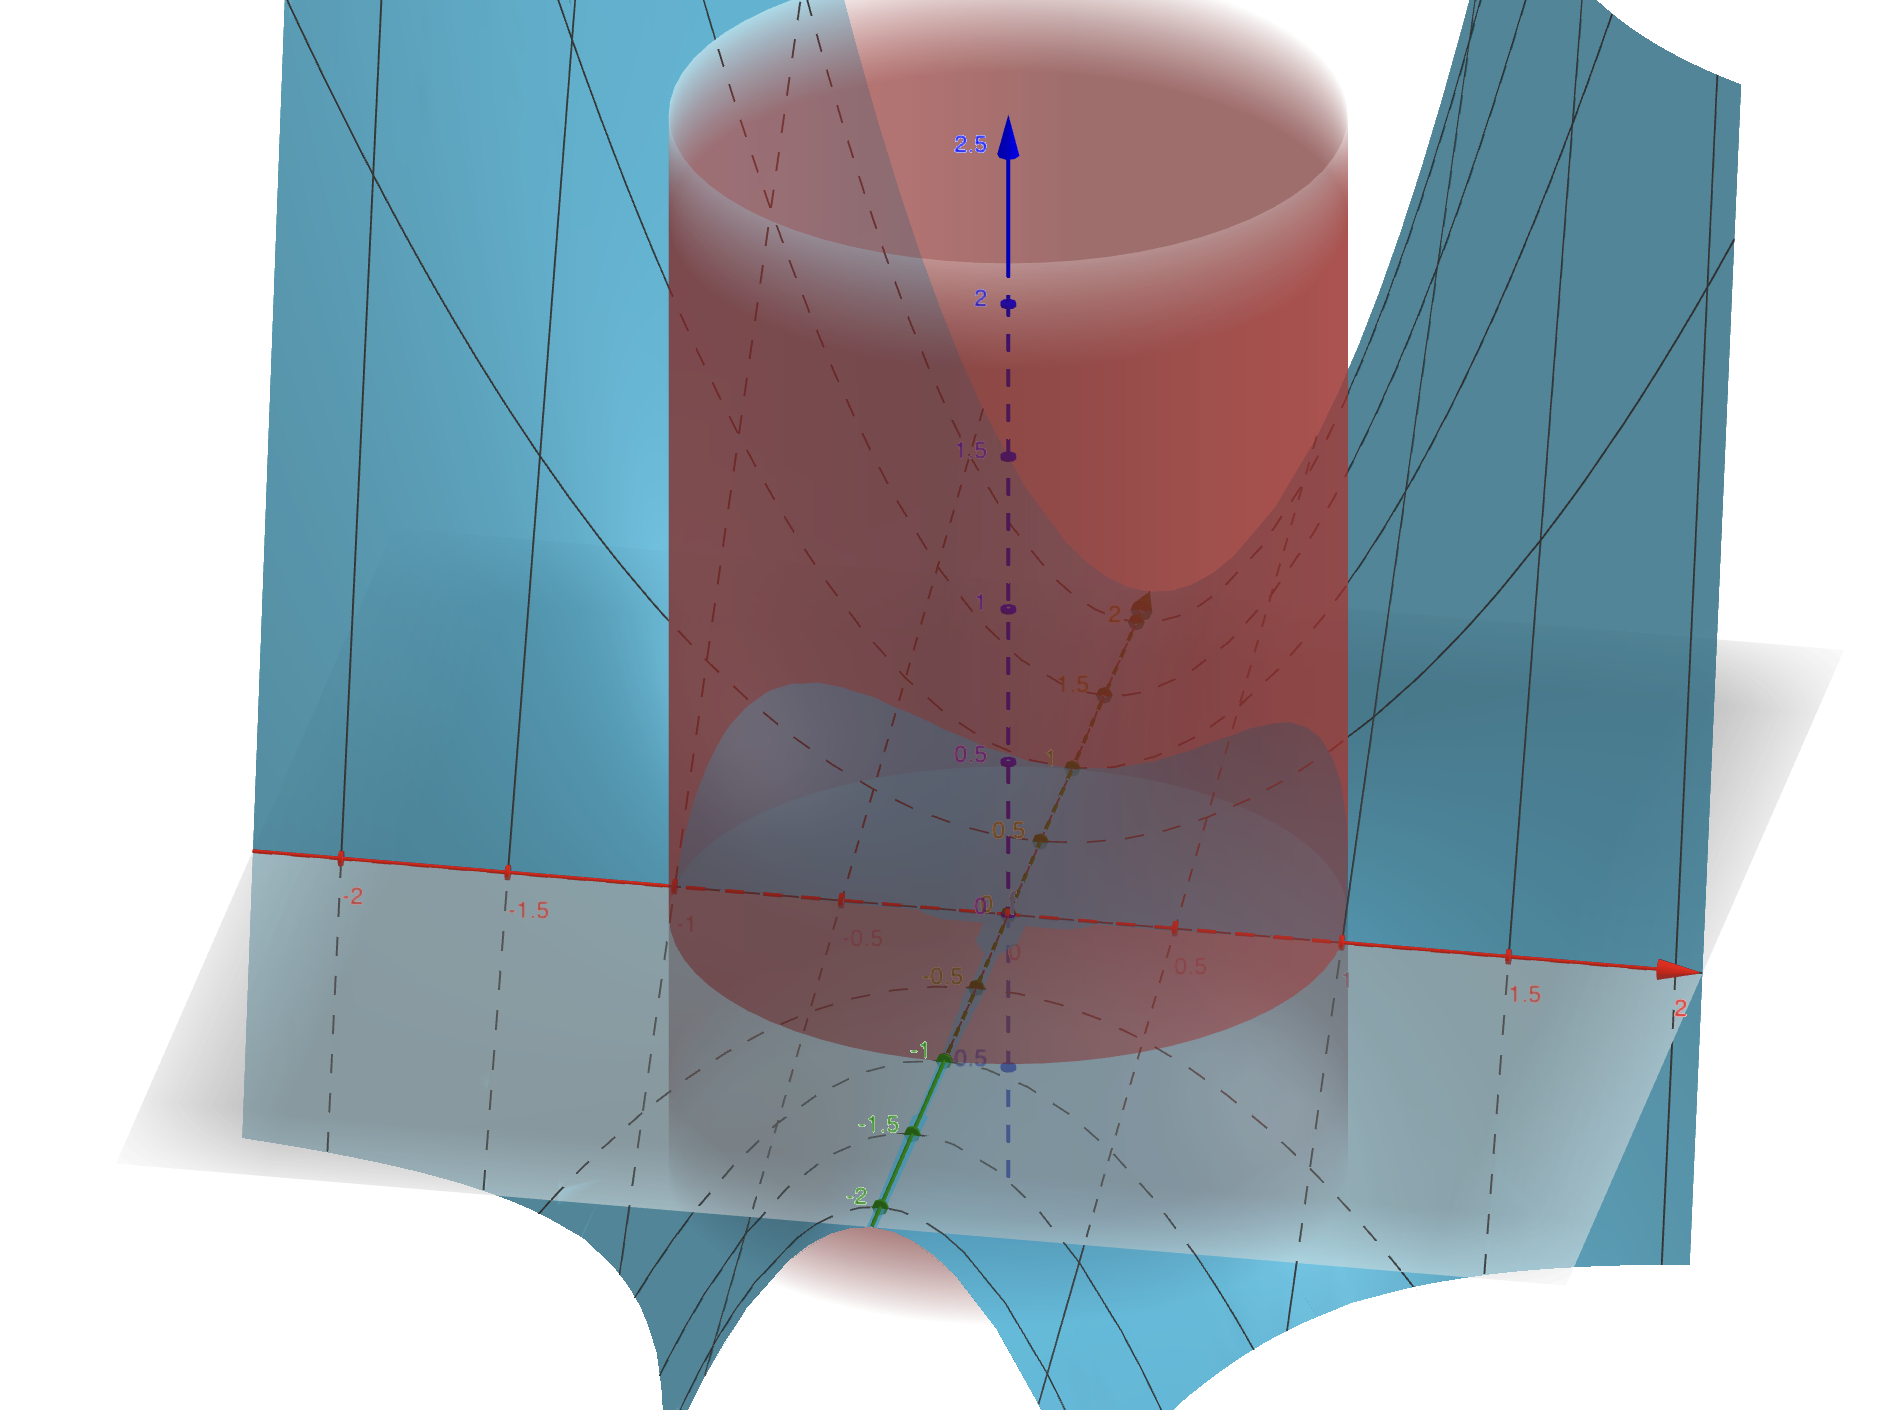
\includegraphics[scale=0.3]{images/Screen Shot 2022-10-26 at 15.13.16.png}
        \caption{$f(x,y)=x^2y$ and $x^2+y^2=1$}
    \end{figure}
\end{itemize}
\noindent \textbf{Remark}:
\begin{itemize}
    \item If the constrain is $g(x_1,\cdots,x_n)=(a_1,\cdots,a_m)$ for $(a_1,\cdots,a_m)\in \R^m$. Then this constrain can be viewed as 
    $$g_1(x_1,\cdots,x_n)=a_1,\cdots,g_m(x_1,\cdots,x_n)=a_m$$
\end{itemize}
\chapter{Integration}

\section{Reimann Integral over a Rectangle}

\begin{definition}
    Consider a rectangle $Q=[a_1,b_1]\times [a_2,b_2]\times \cdots \times[a_n,b_n]\subset \R^n$.
    \begin{itemize}
        \item Each of the interval $[a_i,b_i]$ is called a \underline{component interval} of $Q$.
        \item $\max\{b_1-a_1,b_2-a_2,\cdots ,b_n-a_n\}$ is called the \underline{width} of $Q$.
        \item $v(Q)=(b_1-a_1)\times(b_2-a_2)\times \cdots \times(b_n-a_n)$ is called the \underline{volume} of $Q$.
    \end{itemize}
\end{definition}
\noindent \textbf{Remark}:
\begin{itemize}
    \item In the case $n = 1$, the volume and the width of the (1-dimensional)
    rectangle $[a, b]$ are the same, namely, the number $b-a$. This number is also called the \underline{length} of $[a, b]$.    
\end{itemize}

\begin{definition}
    Given a closed interval $[a, b]$ of $\R$, a \underline{partition} of $[a, b]$ is a finite collection $P$ of points of $[a, b]$ that includes the points $a$ and $b$.
    $$P=\{a=t_0,t_1\cdots,t_{k-1},t_k=b\}$$
    where $t_i$ are in increasing order for convenience. Each interval $[t_{i-1},t_i]$ is called a \underline{subinterval} determined by $P$ of the interval $[a,b]$.
\end{definition}

\begin{definition}
    Let $Q=[a_1,b_1]\times [a_2,b_2]\times \cdots \times[a_n,b_n]\subset \R^n$. A \underline{partition} $P$ of $Q$ is an n-tuple $$P=(P_1,P_2,\cdots,P_n)$$ where each $P_i$ is a partition of $[a_i,b_i]$ for each $i$. 
    If for each $i$, $I^{(i)}_j$ is one of the subintervals determined by $P_i$ of the interval $[a_i,b_i]$, then the rectangle $$R=I^{(1)}_{j_1}\times I^{(2)}_{j_2}\times \cdots \times I^{(n)}_{j_n}$$ is called a \underline{subrectangle} determined by $P$, of the rectangle $Q$. 
    The maximum width of these subrectangles is called the \underline{mesh} of $P$.
\end{definition}

\begin{definition}
    Let $Q\subset \R^n$ be a rectangle and let $f:Q\longrightarrow \R$. Assume $f$ is bounded. Let $P$ be a partition of $Q$. For each subrectangle $R$ determined by $P$, define
    $$m_R(f)=\inf\{f(x): x\in R\}$$
    $$M_R(f)=\sup\{f(x): x\in R\}$$
\end{definition}

\begin{definition}
    Similar to single variable calculus, we can define the \underline{lower sum} and the \underline{upper sum} respectively of $f$ determined by $P$,
    $$L(f,P)=\sum_Rm_R(f)\cdot v(R)$$
    $$U(f,P)=\sum_RM_R(f)\cdot v(R)$$
    where the summations extend over all subrectangles $R$ determined by $P$.
\end{definition}

\begin{definition}
    Let $P=(P_1,P_2,\cdots,P_n)$ and $P'=(P_1',P_2',\cdots,P_n')$ be partitions of $Q$.
    \begin{itemize}
        \item If $P_i \subset P_i'$ for all $i$, then $P'$ is called a \underline{refinement} of $P$.
        \item Can also define a new partition based on $P$ and $P'$,
        $$P''=(P_1 \cup P_1',P_2\cup P_2',\cdots,P_n\cup P_n')$$
        $P''$ is called the \underline{common refinement} of $P$ and $P'$.
    \end{itemize}
\end{definition}

\begin{lemma}
    Let $P=(P_1,P_2,\cdots,P_n)$ and $P'=(P_1',P_2',\cdots,P_n')$ be partitions of $Q\subset \R^n$ and $P'$ refines $P$. Let $f:Q\longrightarrow \R$. Then we have
    $$L(f,P)\leq L(f,P') \text{ and }U(f,P')\leq U(f,P)$$
\end{lemma}


\begin{lemma}
    Let $Q$ be a rectangle; let $f:Q\longrightarrow R$ be a bounded function. If $P$ and $P'$ are any two partitions of $Q$, then
    $$L(f,P)\leq U(f,P')$$
\end{lemma}


\begin{theorem}
    Let $P=(P_1,P_2,\cdots,P_n)$ and $P'=(P_1',P_2',\cdots,P_n')$ be partitions of $Q\subset \R^n$ and $P'$ refines $P$. Let $f:Q\longrightarrow \R$. Then we have
    $$L(f,P)\leq L(f,P') \leq U(f,P')\leq U(f,P)$$
\end{theorem}

\begin{definition}
    Let $Q\subset \R^n$ be a rectangle. Let $f:Q\longrightarrow \R$ be a bounded function. Let $\mathcal{P}$ denotes the set of all partitions of $Q$.
    \begin{itemize}
        \item \underline{Lower integral}: $$\underline{\int_Q}f=\sup\{L(f,P):P\in\mathcal{P}\}$$
        \item \underline{Upper integral}: $$\overline{\int_Q}f=\inf\{U(f,P):P\in\mathcal{P}\}$$
    \end{itemize}
\end{definition}

\begin{definition}
    We say $f$ is \underline{integrable} over $Q$ if the upper and lower integrals of $f$ over $Q$ are equal.
    We denote the integral as $$\int_Qf\text{ or }\int_{x\in Q}f(x)$$
\end{definition}
\noindent \textbf{Remark}:
\begin{itemize}
    \item The lower integral represents the so-called “inner area” of this region, computed by approximating the region by inscribed rectangles, while the upper integral represents the so-called “outer area,” computed by approximating the region by circumscribed rectangles. If the “inner” and “outer” areas are equal, then $f$ is integrable.
\end{itemize}
\noindent \textbf{Example}:
\begin{itemize}
    \item If Q is a rectangle in $\R^2$ and $f: Q \longrightarrow \R$ is non-negative and bounded, one can picture $L(f,P)$ as the total volume of a bunch of boxes inscribed in the region between the graph of $f$ and the xy-plane, and $U(f, P)$ as the total volume of a bunch of boxes circumscribed about this region.
    \begin{figure}[ht]
        \centering
        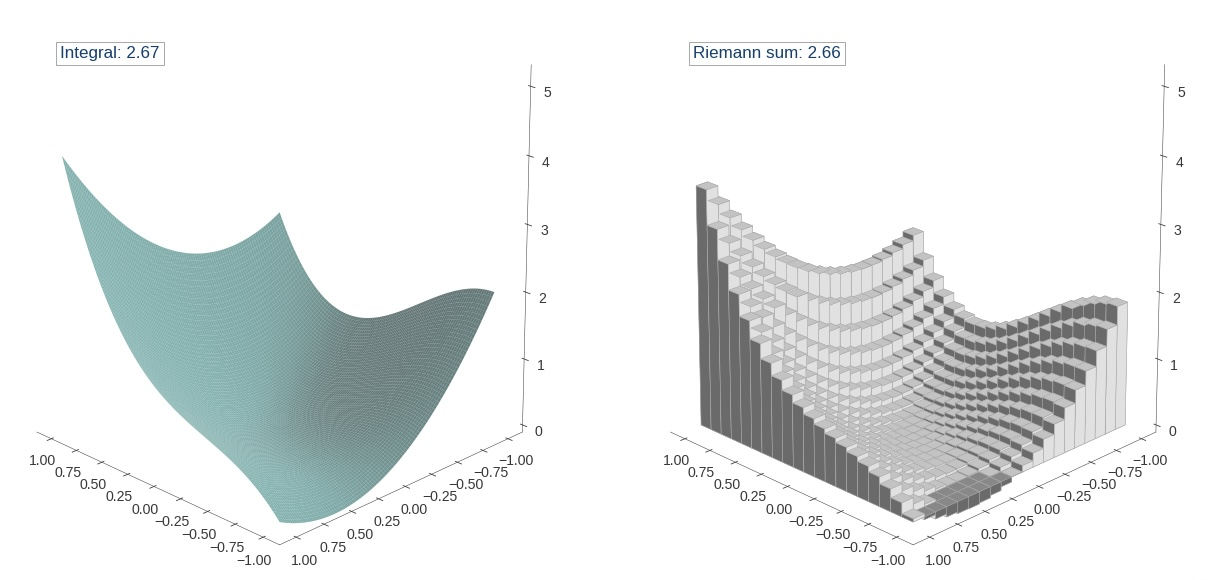
\includegraphics[scale=0.32]{images/fig4031-riemann-integration-multivariate.jpeg}
        \caption{Picture of Reimann sum}
    \end{figure}
\end{itemize}

\begin{theorem}[The Riemann Condition]\label{The Riemann Condition}
    Let $Q\subset \R^n$ be a rectangle, let $f:Q \longrightarrow \R$ be bounded. Let $\mathcal{P}$ be the set of all partitions of $Q$. Then $f$ is integrable if and only if 
    $$\forall \epsilon >0. \exists P \in \mathcal{P}. U(f,P)-L(f,P)<\epsilon$$
\end{theorem}

\begin{theorem}\label{sum of subrectangles}
    Let $Q\subset \R^n$ be a rectangle. Let $\{Q_1,\cdots,Q_k\}$ be a finite collection of rectangles that covers $Q$. Then 
    $$v(Q)\leq \sum_{i=1}^kv(Q_i)$$
\end{theorem}

\begin{theorem}\label{continuous implies integrable}
    Let $Q\subset \R^n$ be a rectangle, let $f:Q \longrightarrow \R$ be continuous. Then $f$ is integrable.
\end{theorem}

\section{Conditions for Integrability}

\begin{definition}
    We say $A\subset \R^n$ has \underline{measure zero} if for any $\epsilon>0$, there exists countably many rectangles $\{Q_1,Q_2,\cdots\}$ cover $A$ such that
    $$\sum_{i=1}^{\infty}v(Q_i)<\epsilon$$
    In this case, we say that the \underline{total volume} of the rectangles $Q_1,Q_2,\cdots$ is less than $\epsilon$.
\end{definition}

\begin{theorem}\ \label{measure zero 4 theorems}
    \begin{enumerate}
        \item If $B \subset A$ and $A$ has measure zero in $\R^n$, then so does $B$.
        \item All of $A_1,A_2,\cdots$ has measure zero in $\R^n$. Then $A=\bigcup_{i=1}A_i$ has measure zero in $\R^n$.
        \item A set $A$ has measure zero in $\R^n$ if and only if for every $\epsilon > 0$, there is a countable covering of $A$ by open rectangles $Int(Q_1), Int(Q_2),\cdots$ such that $$\sum_{i=1}^{\infty}v(Q_i)<\epsilon$$
        \item If $Q$ is a rectangle in $\R^n$, then $Bd(Q)$ has measure zero in $\R^n$ but $Q$ does not.
    \end{enumerate}
\end{theorem}

\noindent \textbf{Example}:
\begin{itemize}
    \item The \underline{cantor set} in $[0,1]$ is created by iteratively deleting the open middle third from a set of line segments
    \begin{itemize}
        \item $C_0:= [0,1]$
        \item $C_n:=\frac{C_{n-1}}{3}\cup (\frac{2}{3}+\frac{C_{n-1}}{3})$
    \end{itemize}
    So the formal definition of the cantor set is $$\mathcal{C}:=\lim_{n\to \infty}C_n=\bigcap_{n=1}^{\infty}C_n$$
    \begin{figure}[ht]
        \centering
        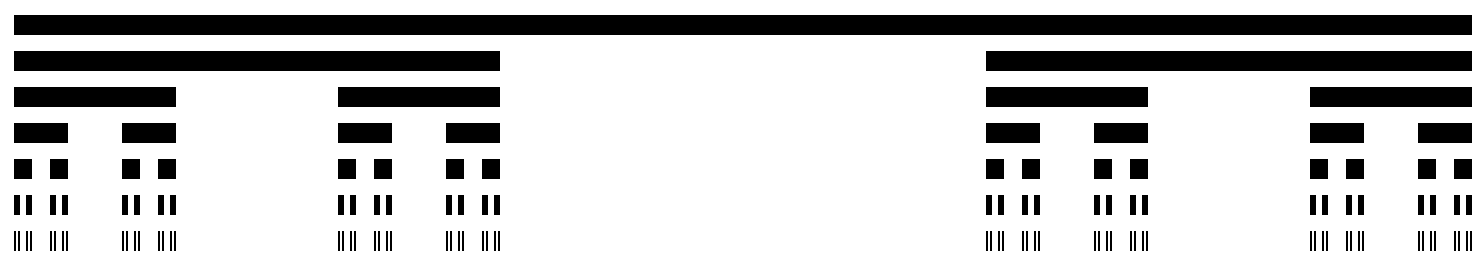
\includegraphics[scale=0.5]{images/cantor set.png}
        \caption{Picture of creating the cantor set}
    \end{figure}
    \underline{The fact is that the cantor set has measure zero.}
    \item Every k-dimensional subspace of $\R^n$ has measure zero if $k < n$. In other words, lines have no area, and planes have no volume. For example, the two dimensional sphere $\mathbb{S}^2$ has measure zero in $\R^3$.
\end{itemize}

\begin{definition}
    Let $Q$ be a rectangle in $\R^n$. Let $f:Q\longrightarrow \R$. $\forall a \in Q.\forall \delta>0$ let
    $$A_{\delta}=\{f(x): x\in Q \text{ and }x \in U(a;\delta)\}$$
    Also, we let
    $$M_{\delta}(f)=\sup A_{\delta}$$
    $$m_{\delta}(f)=\inf A_{\delta}$$
    Now we can define the \underline{oscillation} of $f$ at $a$ by the equation
    $$v(f;a):=\inf\{M_{\delta}(f)-m_{\delta}(f): \delta >0\}$$
    It is clear that $v(f;a)\geq 0$ always hold.
\end{definition}

\begin{lemma}
    $f$ is continuous at $a$ if and only if $v(f;a)=0$.
\end{lemma}


\begin{theorem} \label{bounded f integrable iff D measure zero}
    Let $Q$ be a rectangle in $\R^n$, let $f : Q \longrightarrow R$ be a bounded function. Let $D$ be the set of points of $Q$ at which $f$ fails to be continuous. Then $f$ is integrable if and only if $D$ has measure zero in $\R^n$.
\end{theorem}

\begin{theorem}
    Let $Q\subset \R^n$ be a rectangle. Let $f:Q\longrightarrow \R$. Assume $f$ is integrable on $Q$. Then
    \begin{enumerate}
        \item If $f$ vanishes except on a set of measure zero, then $\int_Qf=0$.
        \item If $f$ is non-negative and if $\int_Qf=0$, then $f$ vanishes except on a set of measure zero.
    \end{enumerate}
\end{theorem}

\section{Evaluation of Reimann Integral}

\begin{theorem}[Fundamental Theorem of Calculus]\label{FTC}\
    \begin{enumerate}
        \item If $f$ is continuous on $[a,b]$ and $F(x)=\int_a^xf(t)\di t$, then $$F'(x)=f(x)$$
        \item If $f$ is continuous on $[a,b]$ and $F$ is of class $C^2([a,b])$ such that $f(x)=F'(x)$, then $$\int_a^bf(x)\di x=F(b)-F(a)$$
    \end{enumerate}
\end{theorem}
\noindent \textbf{Remark}:
\begin{itemize}
    \item The part 1 of the theorem tells us the anti-derivative of $f$ always exists in theory.
    \item The part 2 of the theorem tells us we can claculate the integral of $f$ if we find the anti-derivative.
    \item The same difficulties of evaluating the integral occur with n-dimensional integrals.
    \item One way of approaching the problem is to attempt to reduce the computation of an n-dimensional integral to the presumably simpler problem of computing a sequence of lower-dimensional integrals.
\end{itemize}

\begin{theorem}[Fubini for continuous functions of two variable] \label{Fubini for continuous functions of two variable}
    Let $Q = [a, b] \times[c,d]\subset \R^2$ be a rectangle. Let $f:Q\longrightarrow \R$ be continuous, then the integral of $f$ over $Q$ is
    $$\int_Qf=\int_{y=c}^{y=d}\left(\int_{x=a}^{x=b}f(x,y)\di x\right)\di y=\int_{x=a}^{x=b}\left(\int_{y=c}^{y=d}f(x,y)\di y\right)\di x$$
\end{theorem}

\begin{figure}[ht]
    \centering
    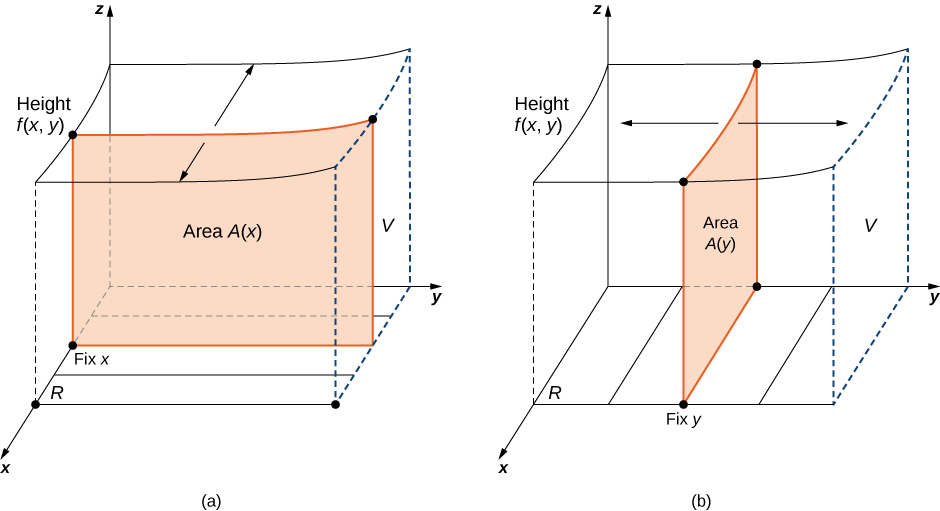
\includegraphics[scale=0.8]{images/CNX_Calc_Figure_15_01_006.jpg}
\end{figure}

\begin{theorem}[Fubini for continuous functions of n variable]
    Let $Q=[a_1,b_1]\times\cdots\times[a_n,b_n]\subset \R^n$ be a rectangle. Let $f:Q\longrightarrow \R$ be continuous. Then
    $$\int_Qf=\int_{x_1=a_1}^{x_1=b_1}\left[\int_{x_2=a_1}^{x_2=b_2}\left(\cdots\left(\int_{x_n=a_n}^{x_n=b_n}f(x_1,x_2,\cdots,x_n)\di x_n\right) \cdots \right)\di x_2\right]\di x_1$$
    and the order of the integration can be arbitrarily changed.
\end{theorem}

\noindent \textbf{Example}:
Let $Q=[0,\pi]\times[1,2]$, let $f(x,y)=sin(x)+y^2e^x$. Then
    \begin{equation}
        \begin{split}
            \int_Qf &= \int_{x=0}^{x=\pi}\left(\int_{y=1}^{y=2}(sin(x)+y^2e^x)dy\right)\di x\\
            &= \int_{x=0}^{x=\pi}\left(sin(x)y+\frac{y^3}{3}e^x\right)\Big|_1^2\di x\\
            &= \int_{x=0}^{x=\pi}\left(sin(x)+\frac{7}{3}e^x\right)\di x\\
            &= \left(-cos(x)+\frac{7}{3}e^x\right)\Big|_0^{\pi}\\
            &= \frac{7}{3}e^{\pi}-\frac{1}{3}
        \end{split}
    \end{equation}
\noindent \textbf{Remark}:
\begin{itemize}
    \item The theorems above are all about continuous functions. They are not usually proved in calculus. In fact, it is seldom mentioned that a proof is needed. They are taken as obvious. We can prove them with all the knowledge we have learnt.
    \item Our goal is to generalize these theorems to n-dimensional Euclidean space with integrable functions(may not be continuous). We will even generalize to metric space in the future. We should just prove the most generalized version(Fubini's Theorem).
    \item The following theorem is generalized from the theorem\ref{Fubini for continuous functions of two variable}. It is a corollary of the Fubini's Theorem.
\end{itemize}

\begin{theorem}
    Let $Q=I_1\times I_2\subset \R^2$ where $I_1,I_2$ are closed intervals in $\R$. Let $f:Q\longrightarrow\R$ be bounded. 
    If $\int_Qf$ exists, and if $\int_{y\in I_2}f(x,y)$ exists for each $x \in I_1$, then
    $$\int_Qf=\int_{x\in I_1}\int_{y\in I_2}f(x,y)$$
\end{theorem}

\noindent \textbf{Remark}:
\begin{itemize}
    \item It is possible for $f(x,y)$ to be integrable over $Q$, but $\int_{y\in I_2}f(x,y)$ does not exist for some $x$. Consider the following example: 
    Let $Q=[0,1]\times[0,1]$, define the function $f$ over $Q$
    \begin{equation}
        f(x,y)=
        \begin{cases}
            1\text{\quad if $x=0$ and $y$ is rational}\\
            0\text{\quad otherwise}
        \end{cases}
    \end{equation}
    \begin{figure}[ht]
        \centering
        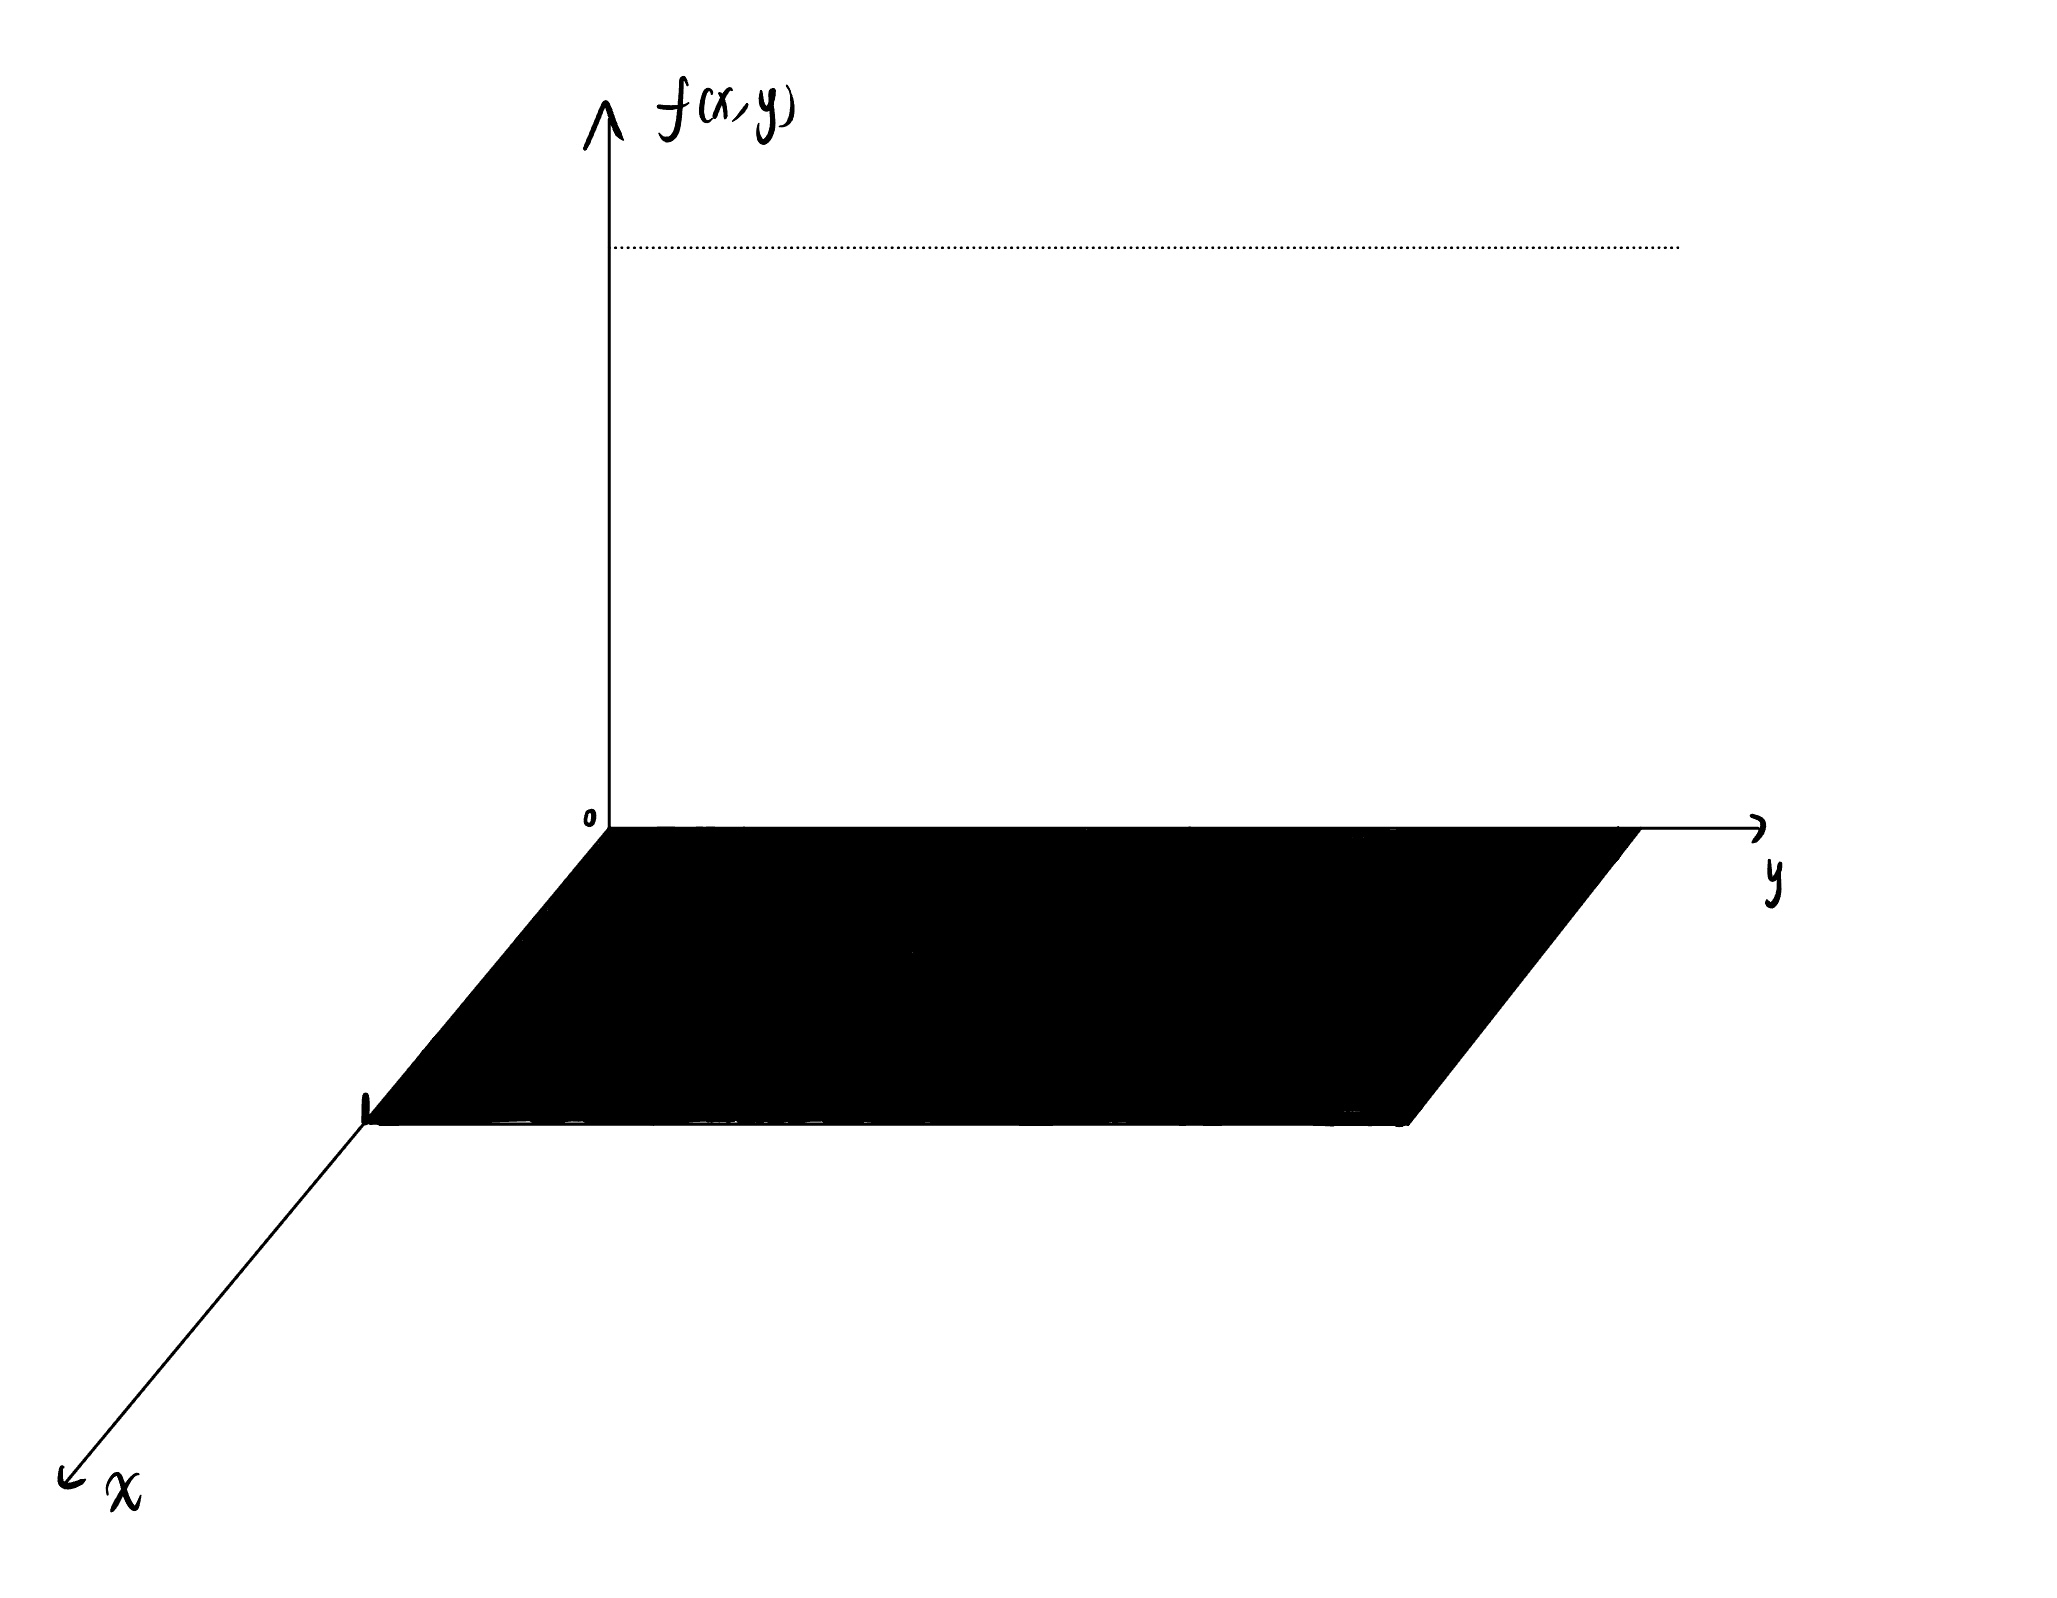
\includegraphics[scale=0.1]{images/IMG_0341.jpeg}
    \end{figure}
    It is clear that $f$ is integrable over $Q$ because the discontinuity set has measure zero. For $x=0$, $\int_{y=0}^{y=1}f(0,y)\di y$ does not exist. But the upper and lower integrals are well-defined
    $$\overline{I}(0)=\overline{\int_{y\in [0,1]}}f(0,y)=1\text{\quad and \quad}\underline{I}(0)=\underline{\int_{y\in [0,1]}}f(0,y)=0$$
    Now we notice that
    $$\int_Qf=\int_{x=0}^{x=1}\overline{I}(x)\di x=\int_{x=0}^{x=1}\underline{I}(x)\di x=0$$
    \item Actually, we can still generalize this theorem, which is the Fubini for $\R^2$.
\end{itemize}

\begin{theorem}[Fubini for $\R\times\R$]
    Let $Q=I_1\times I_2\subset \R^2$ where $I_1,I_2$ are closed intervals in $\R$. Let $f:Q\longrightarrow\R$ be bounded. 
    If $\int_Qf$ exists. For each $x$, consider the lower and upper integrals
    $$\overline{\int_{y\in I_2}}f(x,y)\text{\quad and \quad}\underline{\int_{y\in I_2}}f(x,y)$$
    These two functions of $x$ are integrable, and
    $$\int_Qf=\int_{x\in I_1}\overline{\int_{y\in I_2}}f(x,y)=\int_{x\in I_1}\underline{\int_{y\in I_2}}f(x,y)$$
\end{theorem}

\noindent \textbf{Remark}:
\begin{itemize}
    \item Before we get into the full Fubini's theorem, we will make clear the following definitions.
    \item We should keep in mind that we only defined the integral of functions from closed rectangle in $\R^n$ to $\R$.
\end{itemize}

\begin{definition}
    Let $Q=I_1\times\cdots\times I_m\times J_1\times\cdots \times J_n$ be a closed rectangle in $R^{m+n}$ where all $I_i$ and $J_k$ are closed interval. Let $Q_1=I_1\times \cdots \times I_m$ be a closed rectangle in $\R^m$ and $Q_2=J_1\times\cdots\times J_n$ be a closed rectangle in $\R^n$.
    We define
    $$Q=Q_1\times Q_2$$
    In particular, we have $$\R^{m+n}=\R^m\times \R^n$$
    Also, let $A\subset \R^m$, $B\subset\R^n$, $C\subset \R^p$ be closed rectangles, then $$(A\times B)\times C=A\times (B\times C)$$
    For $c=(x_1,\cdots,x_m,y_1,\cdots,y_n)\in \R^{m+n}$, let $x=(x_1,\cdots,x_m)\in \R^m$, $y=(y_1,\cdots,y_n)\in \R^m$, we write $$c=(x,y)\in \R^{m+n}$$
\end{definition}

\noindent \textbf{Remark}:
\begin{itemize}
    \item I admit that this is an abuse of notations. The above we defined is the product of subsets of $\R^n$, not the cartesian product of arbitrary sets.
    \item In view of set theory(cartesian product of sets), $$\R^{m+n}\neq\R^m\times\R^n$$
    But the difference is very subtle. To be precise $$\R^{m+n}=U\oplus V$$
    where $$U=\{(x_1,\cdots,x_m,0,\cdots,0):(x_1\cdots,x_m)\in \R^m\}$$
    $$V=\{(0,\cdots,0,y_1,\cdots,y_n):(y_1\cdots,y_n)\in \R^n\}$$
    The subspaces $U$ and $V$ looks exactly like $\R^m$ and $\R^n$. $U\oplus V$ and $\R^m\times \R^n$ are not only isomorphic, they are called \underline{canonically isomorphic}. It is like the relation of the vector space $V$ and its double dual space $V^{**}$.
    \item Our definition means whenever we are in spaces like $\R^{m+n}$, we can view it as a hyperplane where the two hyperlines looks exactly like $\R^m$ and $\R^n$.
\end{itemize}

\begin{theorem}[Full Fubini]
    Let $f : Q\subset\R^{m+n} \longrightarrow \R$ be a bounded function and $Q = A \times B$ a rectangle as defined above where $A\subset\R^m$ and $B\subset \R^n$.
    We write $f = f(x,y)$, where $x \in A$, and $y \in B$. Fixing $x \in A$, $f(x,y)$ is a function of $y$. Since this function is bounded, the lower and upper integrals are defined.
    $$\underline{I}(x)=\underline{\int_{y\in B}}f(x,y)$$
    $$\overline{I}(x)=\overline{\int_{y\in B}}f(x,y)$$
    Note that $\underline{I}(x) \leq \overline{I}(x)$. The Fubini Theorem concludes the following: If $f$ is integrable over $Q$, then $\underline{I}(x)$ and $\overline{I}(x)$ are integrable over $A$ and
    $$\int_Qf=\int_{x\in A}\underline{I}(x)=\int_{x\in A}\overline{I}(x)$$
\end{theorem}

\section{Riemann Integral over Bounded Sets}

\noindent \textbf{Motivation}:
\begin{itemize}
    \item In reality, we often encounter questions like computing the mass of an object $M$ which is not a simple rectangle. Given the density function $\rho(x,y,z)$, we should integrate $\rho$ over $M$.
    \item We should generalize the definition of integral over a bouded set.
\end{itemize}

\begin{definition}
    Let $S$ be a bouded set in $\R^n$. Let $f:S\longrightarrow \R$ be a bounded function. Define $f_S:\R^n\longrightarrow\R$ by the following
    \begin{equation}
        f_S(x)=
        \begin{cases}
            f(x)\text{\quad for } x\in S\\
            0\text{\quad otherwise}
        \end{cases}
    \end{equation}
    Choose a rectangle $Q$ containing $S$. We define the \underline{integral of $f$ over $S$} by the following
    \begin{equation}
        \int_Sf=\int_Qf_S
    \end{equation}
    provided the latter integral exists.
\end{definition}
\noindent \textbf{Remark}:
\begin{itemize}
    \item We must show that $\int_Sf$ is independent of the choice of $Q$.
    \item We will prove this by the following lemma.
\end{itemize}

\begin{lemma}
    Let $Q$ and $Q'$ be two rectangles in $\R^n$. Let $f:\R^n\longrightarrow\R$ be a bounded function that vanishes outside $Q\cap Q'$, then $f$ is integrable over $Q$ if and only if $f$ is integrable over $Q'$. and
    $$\int_Qf=\int_{Q'}f$$
\end{lemma}


\begin{lemma}
    Let $S\subset \R^n$. Let $f,g:S\longrightarrow \R$. Define 
    $$M=\max\{f(x),g(x)\} \text{\quad and \quad}m=\min\{f(x),g(x)\}$$ 
    Then we have:
    \begin{enumerate}
        \item If $f$ and $g$ are continuous at $x_0$, then $M$ and $m$ are also continuous at $x_0$.
        \item If $f$ and $g$ are integrable over $S$, then $M$ and $m$ are integrable over $S$.
    \end{enumerate}
\end{lemma}


\begin{theorem}[Properties of integral] \label{properties of integral}
    Let $S\subset \R^n$ be bounded. Let $f,g:\longrightarrow \R$ be bounded functions.
    \begin{enumerate}
        \item (Linearity) If $f$ and $g$ are integrable over $S$, then $af+bg$ is integrable over $S$ where $a,b$ are coefficients in $\R$. And we have the formula $$\int_S(af+bg)=a\int_Sf+b\int_Sg$$
        \item (Comparison) Suppose $f$ and $g$ are integrable over $S$.
        \begin{enumerate}
            \item If $\forall x \in S.f(x)\leq g(x)$, then $$\int_Sf\leq \int_Sg$$
            \item $|f|$ is also integrable over $S$ and $$\left|\int_Sf\right|\leq \int_S|f|$$
        \end{enumerate}
        \item (Monotonicity) Let $T\subset S$. If $f$ is non-negative on $S$ and integrable over $T$ and $S$, then $$\int_Tf\leq \int_Sf$$
        \item (Additivity) If $S=S_1\cup S_2$ and $f$ is integrable over $S_1$ and $S_2$, then $f$ is integrable over $S$ and $S_1\cap S_2$. And we have the equation $$\int_Sf=\int_{S_1}f+\int_{S_2}f-\int_{S_1\cap S_2}f$$
    \end{enumerate}
\end{theorem}


\begin{corollary}
    Let $S_1,\cdots,S_k$ be bouded sets in $\R^n$. Assume $S_i\cap S_j$ has measure zero whenever $i\neq j$. Let $S=S_1\cup\cdots\cup S_k$. If $f$ is integrable over each $S_i$, then $f$ is integrable over $S$ and $$\int_Sf=\int_{S_1}f+\cdots+\int_{S_k}f$$
\end{corollary}

\noindent \textbf{Remark}:
\begin{itemize}
    \item Our primary interest is studying the integral of the continuous function $f:S\longrightarrow\R$.
    \item By definition, we find any rectangle $Q$ containing $S$ and extend $f$ to the function $f_S:Q\longrightarrow\R$, then it is reduced to the integral over a rectangle. We know that $f_S$ is integralable over $Q$ iff the set of points $D$ where $f_S$ fails to be continuous has measure zero.
    \item When $f:S\longrightarrow\R$ is continuous, the set $D$ should be in the boundary of $S$. So it is convenient for us to find conditions of $S$ in order to make $f$ integrable over $S$.
\end{itemize}

\begin{theorem}\label{f integrable over S iff E has measure zero}
    Let $S$ be a bounded set in $\R^n$. Let $f:S\longrightarrow\R$ be a bounded continuous function. Let $E$ be the set of points $x_0$ of $Bd(S)$ such that $$\lim_{x\to x_0}f(x)\neq 0$$
    $E$ has measure zero if and only if $f$ is integrable over $S$.
\end{theorem}

\begin{theorem}\label{integral over interior}
    Let $S$ be a bounded set in $\R^n$. Let $f:S\longrightarrow \R$ be a bounded continuous function. Let $A=Int(S)$. If $f$ is integrable over $S$, then $f$ is integrable over $A$ and $$\int_Sf=\int_Af$$
\end{theorem}


\begin{theorem*}
    Let $S$ be a bounded set in $\R^n$. Let $f:S\longrightarrow\R$ be a bounded function. Let $D$ be the set of points of $S$ at which $f$ fails to be continuous. Let $E$ be the set of points of $Bd(S)$ at which $$\lim_{x\to x_0}f(x)\neq0$$
    Then $\int_Sf$ exists if and only if $D$ and $E$ have measure zero.
\end{theorem*}
\noindent \textbf{Remark}:
\begin{itemize}
    \item We proved this in homework.
\end{itemize}

\section{Rectifiable Sets}

\begin{definition}
    A bounded set $S\subset \R^n$ is called \underline{rectifiable} (Only for this book) if and only if  the characteristic function 
    \begin{equation}
        \chi_S(x)=\begin{cases}
            1 \text{\quad}x\in S\\
            0 \text{\quad}x\notin S
        \end{cases}
    \end{equation} is integrable. And we define the \underline{(n-dimensional) volume} of $S$ by the equation $$v(S)=\int_S1$$
\end{definition}
\noindent \textbf{Remark}:
\begin{itemize}
    \item The volume is also called \underline{(Jordan) content}
\end{itemize}

\begin{theorem}
    $S\subset \R^n$ is rectifiable if and only if $S$ is bounded and $Bd(S)$ has measure zero.
\end{theorem}
\noindent \textbf{Remark}:
\begin{itemize}
    \item We can see that this theorem is actually a corollary of theorem\ref{f integrable over S iff E has measure zero}.
    \item Theorem\ref{f integrable over S iff E has measure zero} says that given $S$ and $f$, we can check whether $f$ is integrable over $S$. This theorem tells us if $S$ is a rectifiable set, then any continuous bounded function $f$ is integrable over $S$.
    \item I call the rectifiable set $S$ the set at which we can do integration without worries.
\end{itemize}

\noindent \textbf{Example}: Example of bounded set that is not rectifiable.
\begin{itemize}
    \item Define $S=\{p\in \R: p\in \Q \text{ and }p\in (0,1)\}$. We proved in MAT157 that $S$ is countable. So we can write $S$ as $S=\{p_1,p_2,p_3,\cdots\}$ with $p_i<p_{i+1}$. 
    Let $0<a<1$ be given. For each $p_i$, we can choose an open interval $(a_i,b_i)$ of length less than $\frac{a}{2^i}$ that contains $p_i$ and contained in $(0,1)$. Define $$A=\bigcup_{i=1}^{\infty}(a_i,b_i)$$
    We can show $Bd(A)$ does not have measure zero, so $A$ is an bounded open set that is not rectifiable.
\end{itemize}

\begin{theorem}[Properties of rectifiable sets] \label{properties of rectifiable sets}\
    \begin{enumerate}
        \item (Positivity) If $S$ is rectifiable, then $v(S)\geq 0$.
        \item (Monotonicity) If $S_1,S_2$ are rectifiable with $S_1\subset S_2$, then $v(S_1)\leq v(S_2)$.
        \item (Additivity) If $S_1$ and $S_2$ are rectifiable, then $S_1\cup S_2$ and $S_1\cap S_2$ are rectifiable, and $$v(S_1\cup S_2)=v(S_1)+v(S_2)-v(S_1\cap S_2)$$
        \item Suppose $S$ is rectifiable. Then $v(S)=0$ if and only if $S$ has measure zero.
        \item Suppose $S$ is rectifiable, then $Int(S)$ is also rectifiable and $v(S)=v(Int(S))$.
        \item Suppose $S$ is rectifiable. Then if $f:S\longrightarrow\R$ is bounded and continuous, then $f$ is integrable over $S$.
    \end{enumerate}
\end{theorem}

\begin{definition}
    Let $C$ be a compact and rectifiable set in $\R^{n-1}$. Let $\phi,\psi:C\longrightarrow\R$ be continuous functions such that $\forall x\in C. \phi(x)\leq \psi(x)$. The subset $S\subset \R^n$ defined by the equation
    $$S=\{(x,t): x\in C \text{ and }\phi(x)\leq t \leq \psi(x)\}$$ is called a \underline{simple region} in $\R^n$.
    \begin{figure}[ht]
        \centering
        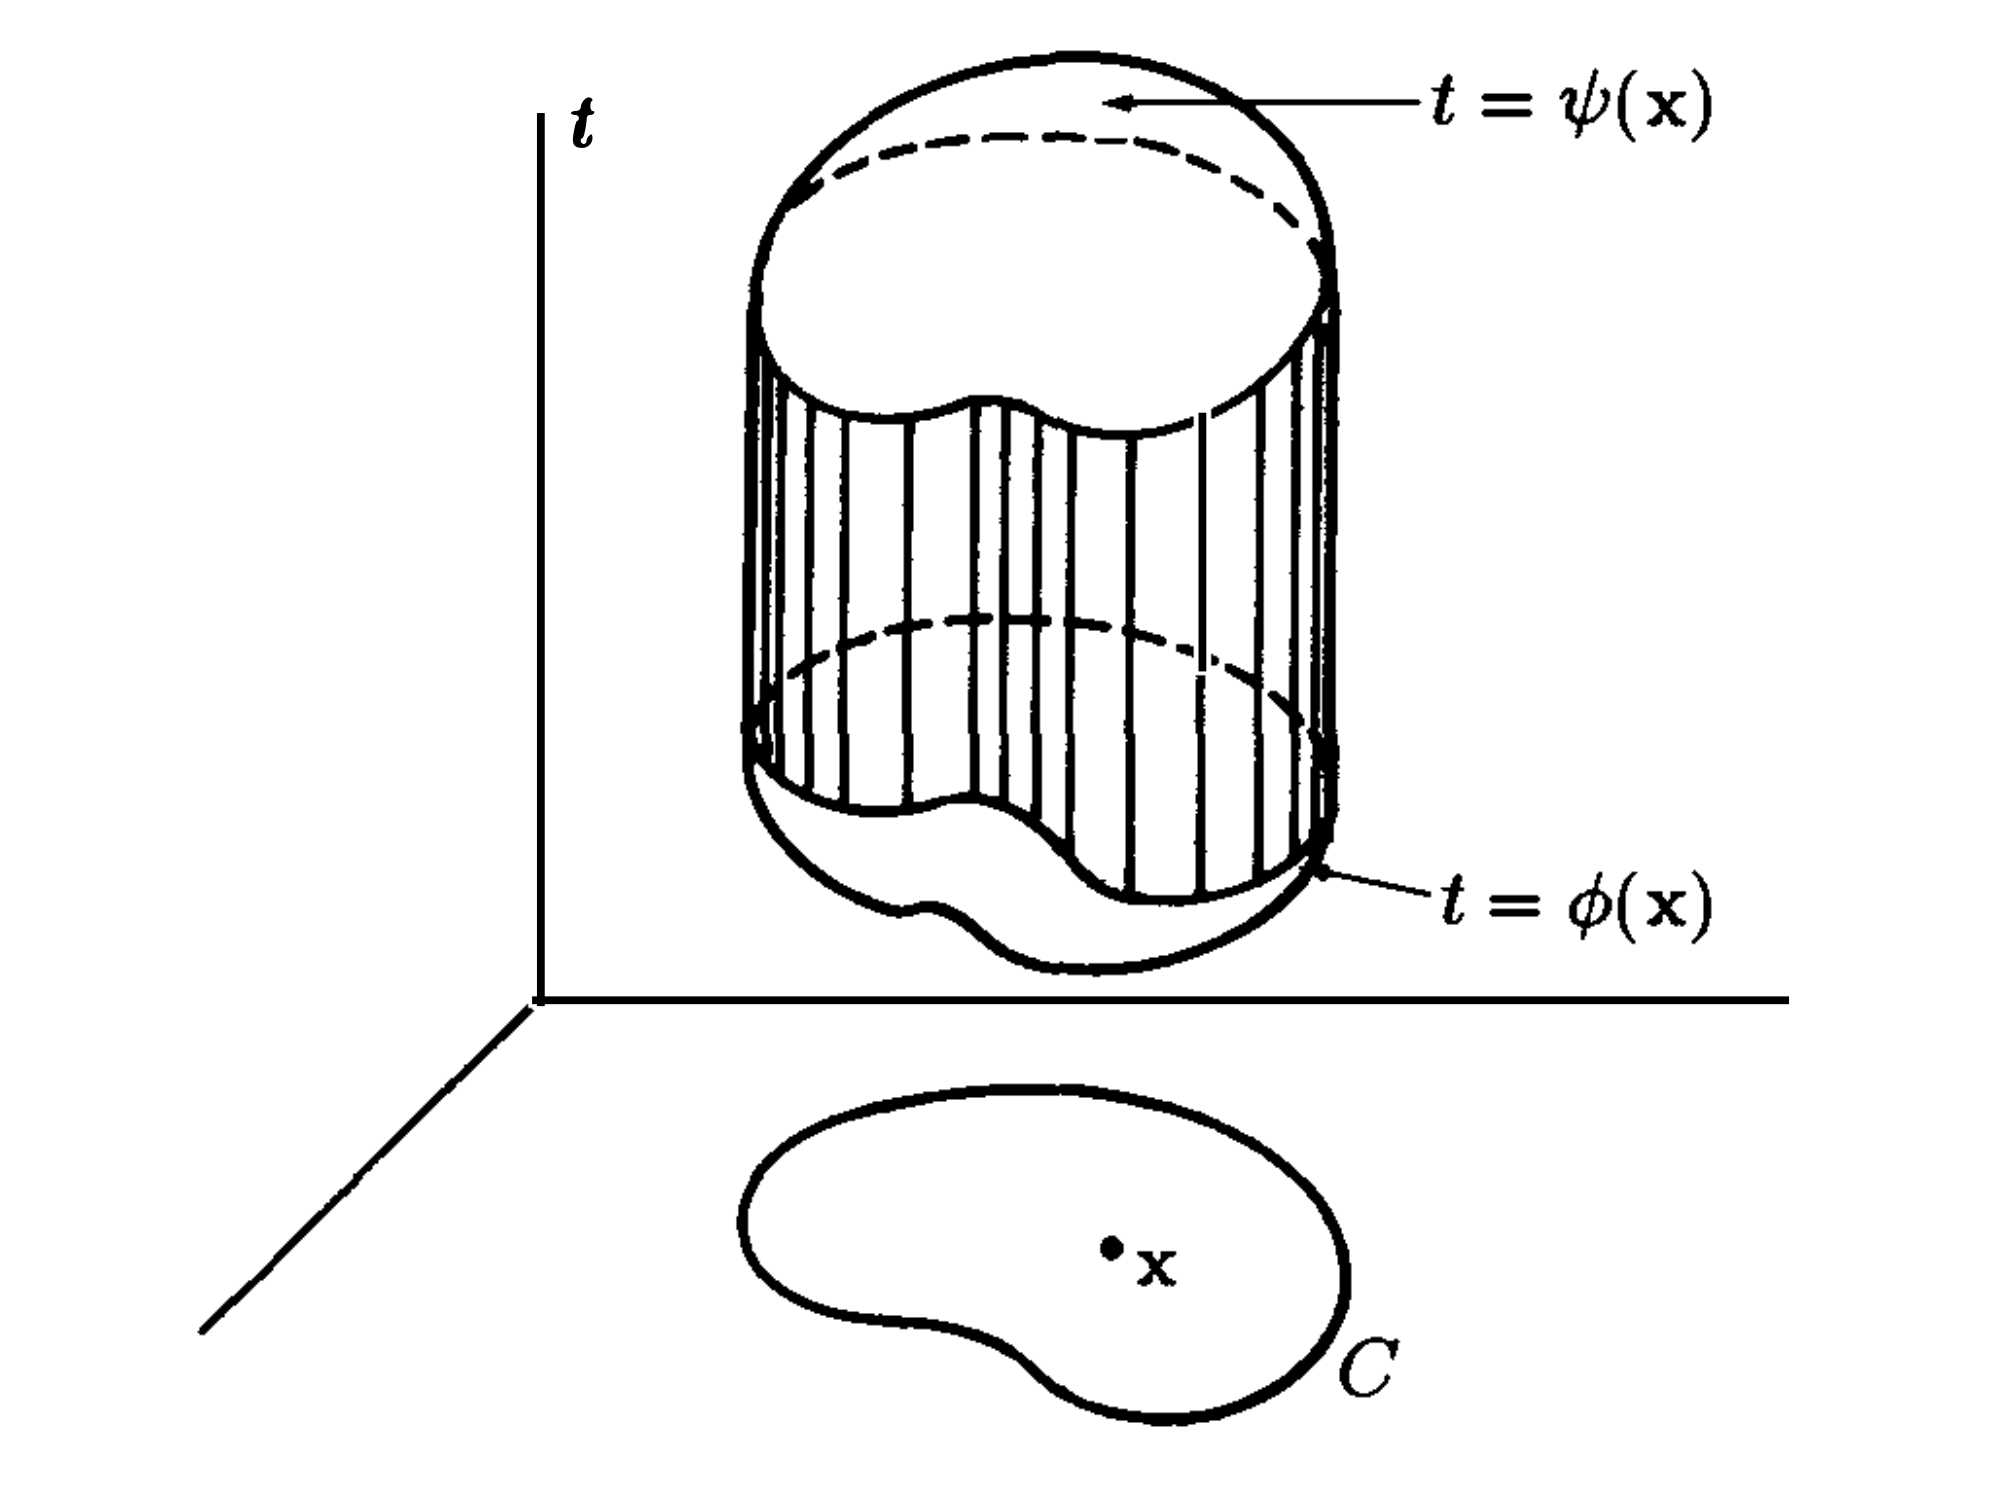
\includegraphics[scale=0.3]{images/Screenshot 2022-11-14 at 17.42.56.png}
        \caption{A picture of simple region in $\R^3$}
    \end{figure}
\end{definition}

\begin{lemma}
    If $S$ is a simple region in $\R^n$, then $S$ is compact and rectifiable.
\end{lemma}

\begin{theorem}[Fubini for simple region]\label{fubini for simple region}
    Let $S$ be a simple region in $\R^n$
    $$S=\{(x,t): x\in C \text{ and }\phi(x)\leq t \leq \psi(x)\}$$
    Let $f:S\longrightarrow\R$ be a continuous function. Then $f$ is integrable over $S$ and $$\int_Sf=\int_C\int_{t=\phi(x)}^{t=\psi(x)}f(x,t)$$
\end{theorem}
\noindent \textbf{Remark}:
\begin{itemize}
    \item This theorem gives us a reasonable method for reducing the n-dimensional integral $\int_Sf$ to lower-dimensional integrals. If $C$ is simple, we can apply this theorem again.
    \item If $S$ is not simple, one can try to exprss $S$ as a union of simple regions that overlap insets of measure zero.
\end{itemize}

\noindent \textbf{Example}:
\begin{itemize}
    \item Consider the set $S=\{(x,y):1\leq x^2+y^2\leq 4\}$.
    \begin{figure}[ht]
        \centering
        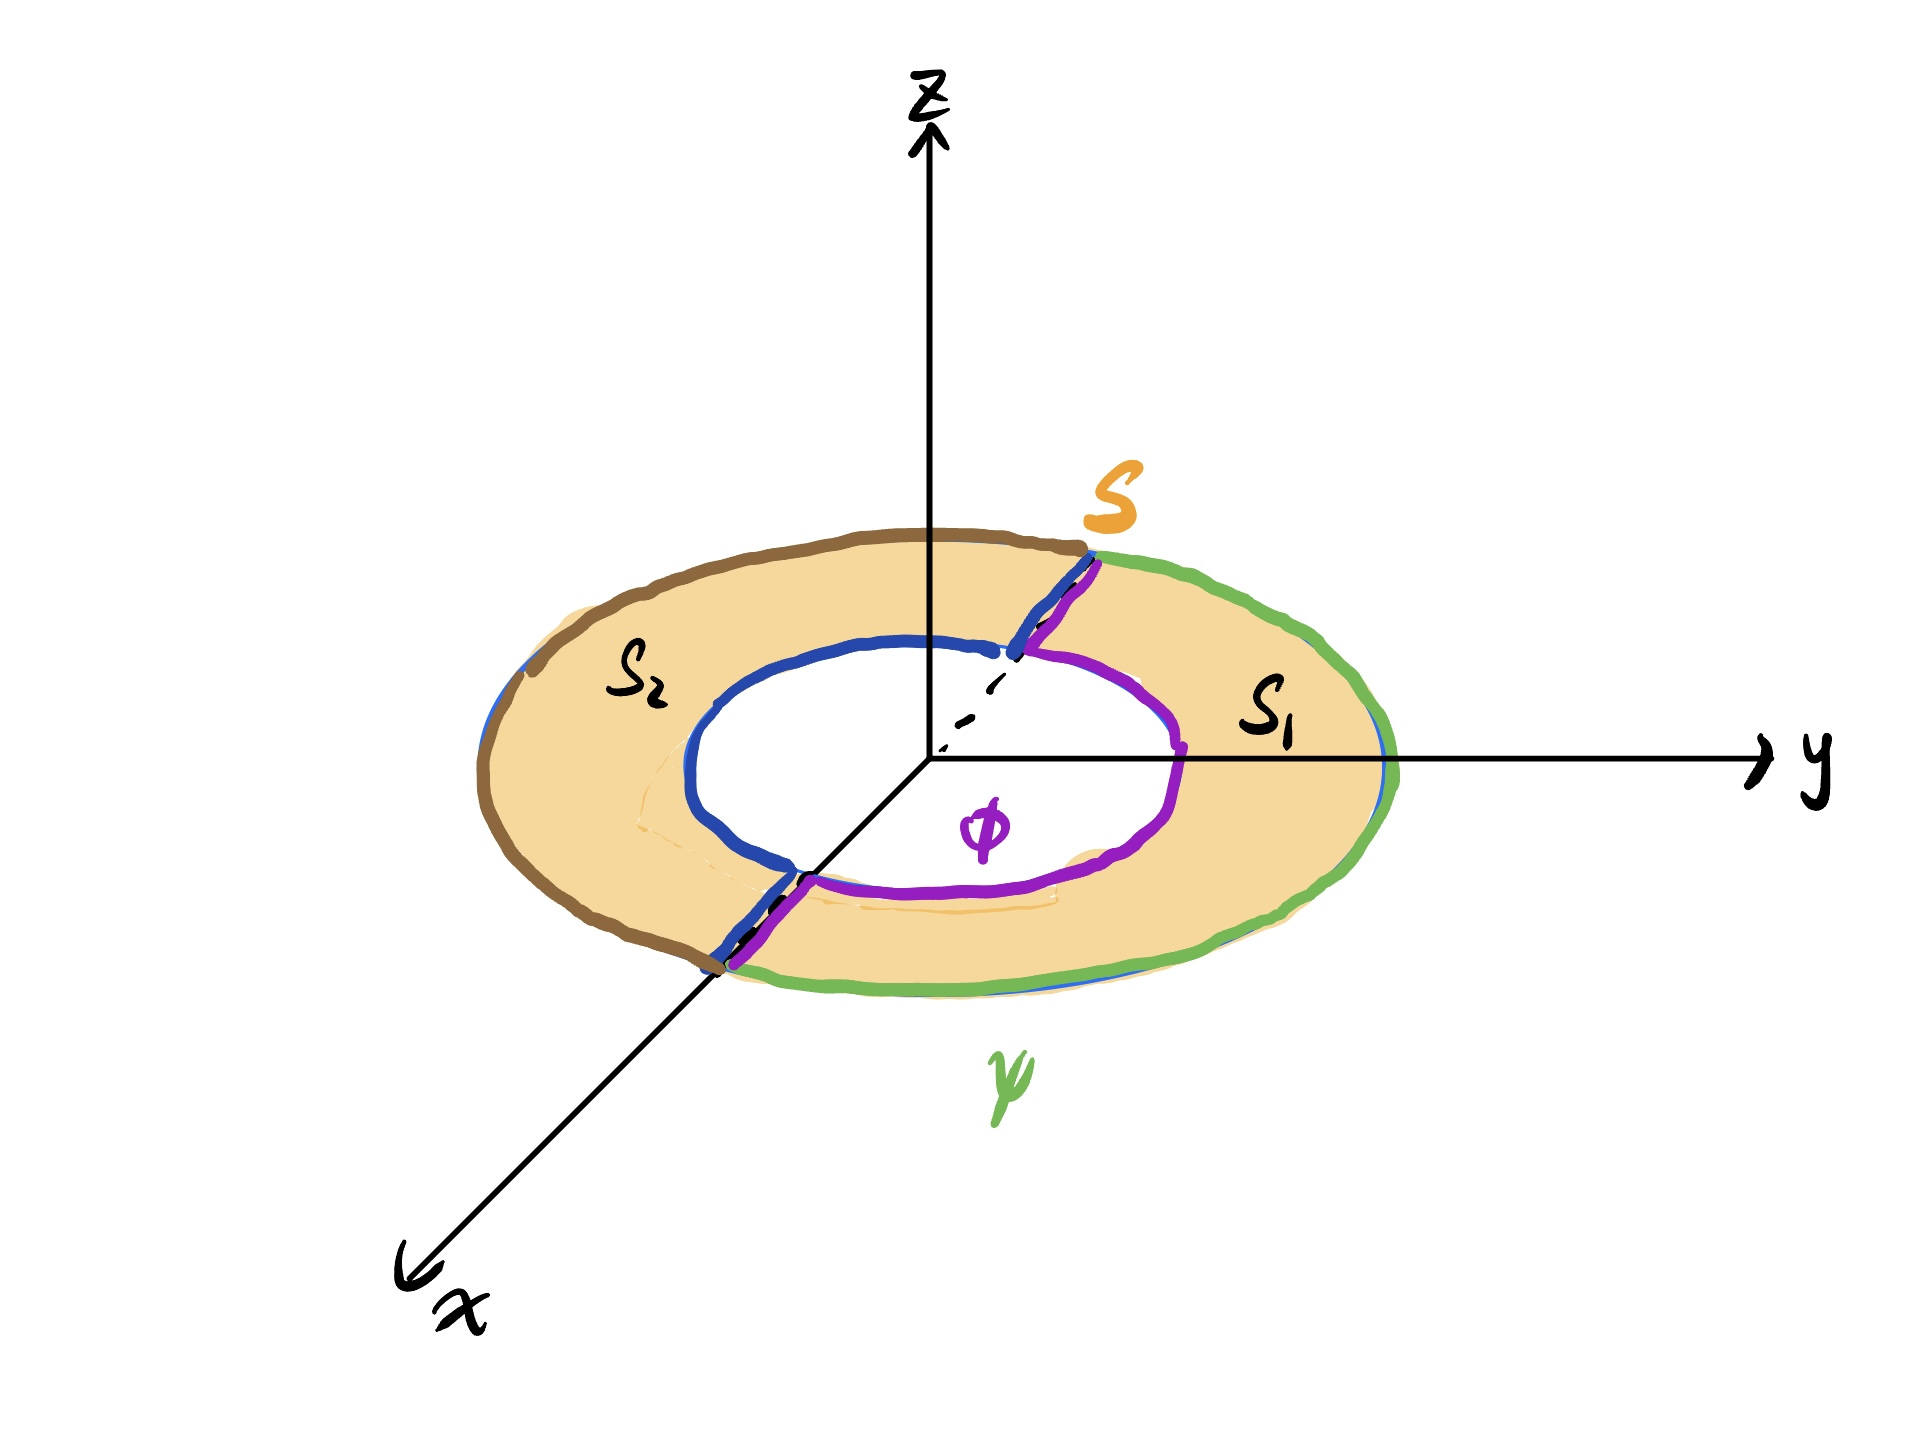
\includegraphics[scale=0.15]{images/IMG_0355.jpg}
        \caption{A picture of $S=\{(x,y):1\leq x^2+y^2\leq 4\}$}
    \end{figure}
    What we want to do is to compute the (Jordan)content of $S$. While $S$ is not a simple region, one can evaluate an integral over $S$ by breaking $S$ up into two simple regions $S_1,S_2$ that overlap in a set of measure zero, as indicated, and integrating over each of these regions separately. Define 
    $$C=[-2,2]$$
    $$\phi(x)=\begin{cases}
        0\text{\quad}x\in[-2,-1]\cup[1,2]\\
        \sqrt{1-x^2}\text{\quad}x\in(-1,1)
    \end{cases}$$
    $$\psi(x)=\sqrt{4-x^2}\text{\quad}x\in C$$
    $$S_1=\{(x,t):x\in C \text{ and }\phi(x)\leq t \leq \psi(x)\}$$
    Since $S_1$ is a simple region, we can apply theorem\ref{fubini for simple region}.
    \begin{equation}
        \begin{split}
            \int_{S_1}1&= \int_C \int_{t=\phi(x)}^{t=\psi(x)}1\\
            &= \int_C t\big|_{\phi(x)}^{\psi(x)}\\
            &= \int_C(\psi(x)-\phi(x))\\
            &= \int_{[-2,2]}\sqrt{4-x^2}-\int_{(-1,1)}\sqrt{1-x^2}\\
            &= 2\pi-\frac{1}{2}\pi\\
            &=\frac{3}{2}\pi
        \end{split}
    \end{equation}
    Similarly, we can compute $$\int_{S_2}1=\frac{3}{2}\pi$$
    Therfore $$\int_S1=\int_{S_1}1+\int_{S_2}1=3\pi$$
    If we encounter a more complex function $f$, and want to integrate $f$ over $S$, another way is to to express the integral in terms of polar coordinates. 
    Expressing a two-dimensional integral in terms of polar coordinates is a special case of a quite general method for evaluating integrals, which is called \underline{substitution} or \underline{change of variables}. We shall deal with it in the next chapter.
\end{itemize}

\section{Improper Integral}

\noindent \textbf{Motivation}:
\begin{itemize}
    \item Up to now, we have studied integrals of bounded functions $f:S\longrightarrow\R$ over bounded sets $S\subset \R^n$.
    \item This is clearly not enough, in this section, we will extend our definition of integral to continuous functions (may not be bounded) $f:A\longrightarrow\R$ to open sets (may not be bounded) $A\subset\R^n$.
\end{itemize}

\begin{definition}
    Let $A\subset\R^n$ be open. Let $f:A\longrightarrow\R$ be continuous. If $f$ is non-negative, i.e.$$\forall x \in A.f(x)\geq0$$
    we define the \underline{(extended) integral} of $f$ over $A$ as $$\int_Af=\sup_{D\subset A}\int_Df$$
    where $D$ is a compact rectifiable subset of $A$, provided this supremum exists. In this case, we say $f$ is \underline{integrable} over $A$ (in the extended sence).
\end{definition}

\begin{definition}
    Generalize the definition above, if $f$ is an arbitrary continuous function over $A$, we consider the non-positive and non-negative parts seperately and turn them into non-negative
    $$f_+(x)=\max\{f(x),0\}$$
    $$f_-(x)=\max\{-f(x),0\}$$
    We say $f$ is \underline{integrable} over $A$  (in the extended sence) if both $\int_Af_+$ and $\int_Af_-$ exist. In this case, we set $$\int_Af=\int_Af_+-\int_Af_-$$
\end{definition}

\noindent \textbf{Remark}:
\begin{itemize}
    \item For $A$ is open and bounded, we now have two definitions of integration. But don't worry, it turns out that if the ordinary integral exists, then the extended integral and the ordinary integral are equal.
    \item But we should notice that sometimes the extended integral exists but the ordinary integral does not. So the extended integral is a more general definition. From now on, $\int_Af$ will denote the extended integral unless specifically stated otherwise.
    \item When $A$ is open in $\R$, this definition of integral is different from the improper integral of single-variable. We show this in the following example.
\end{itemize}

\begin{definition}[Improper integral of single-variable]
    Suppose the restriction of $f:(a,b)\longrightarrow\R$ to any closed subinterval is bounded and integrable. Then we define the \underline{improper integral}:
    $$\int_a^bf=\lim_{x\to a^+}\int_x^cf+\lim_{x\to b^-}\int_c^xf$$
    for any $c\in(a,b)$ provided both limits on right hand exist.
\end{definition}

\noindent \textbf{Example}:
\begin{itemize}
    \item Consider the continuous function $f:(0,\infty)\longrightarrow\R$ defined by $$f(x)=\frac{\sin(x)}{x}$$
    \begin{figure}[ht]
        \centering
        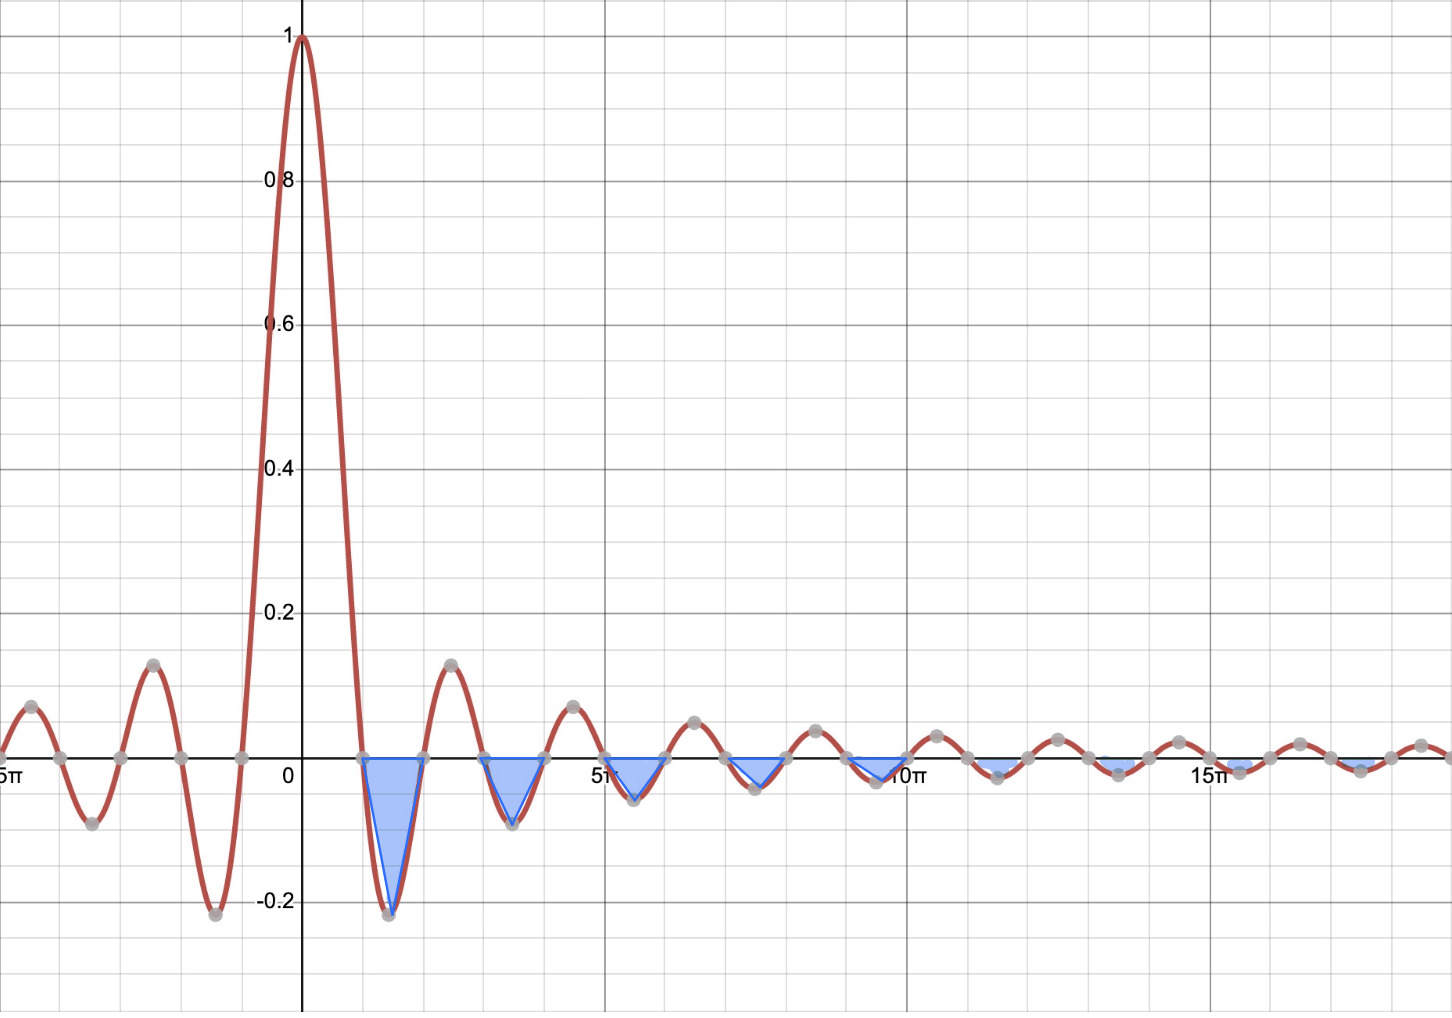
\includegraphics[scale=0.4]{images/Screenshot 2022-11-28 at 04.10.31.png}
        \caption{$f(x)=\frac{\sin(x)}{x}$}
    \end{figure}
    By the definition of improper integral of single-variable, $$\int_0^{\infty}\frac{\sin(x)}{x}\di x=\lim_{a\to 0}\int_{a}^1\frac{\sin(x)}{x}\di x+\lim_{b\to \infty}\int_1^b\frac{\sin(x)}{x}\di x$$
    The first part of RHS exists because for $0<x<1$ $$0<\frac{\sin(x)}{x}<1$$
    The second part of RHS also exists because by integration by parts
    \begin{equation}
        \begin{split}
            \lim_{b\to \infty}\int_1^b\frac{\sin(x)}{x}\di x &= \lim_{b\to \infty}\int_1^b\frac{1}{x}(-\cos(x))'\di x\\
        &= \lim_{b\to \infty}\left(\frac{1}{x}(-\cos(x))\right)\Big|_1^b-\lim_{b\to \infty}\int_1^b\frac{-1}{x^2}\cos(x)\di x\\
        &= \lim_{b \to \infty}\int_1^b\frac{1}{x^2}\cos(x)\di x-\lim_{b \to \infty}\frac{cos(b)}{b}+\cos(1)\\
        & \leq \lim_{b\to \infty}\int_1^b\frac{1}{x^2}\di x-0+cos(1)\\
        &<\infty
        \end{split}
    \end{equation}
    Therefor, the improper integral of $f$ over $(0,\infty)$ exists. Actually, it is equal to $\frac{\pi}{2}$.
    \item For $f$ defined as above. By our definition of (extended) integral, $\int_0^{\infty}\frac{\sin(x)}{x}\di x$ does not exist. Consider $$f_-(x)=\max\left\{-\frac{\sin(x)}{x},0\right\}$$
    It suffices to show that the extended integral of $f_-$ over $(0,\infty)$ does not exist. 
    Intuitively, we want to show that the extended integral of $f_-$ over $(0,\infty)$ is large than the area of these blue triangles.
    \begin{equation}
        f_-(x)=\begin{cases}
            -f(x)\text{\quad }x\in[\pi+2k\pi,2\pi+2k\pi]\\
            0 \text{\quad otherwise}
        \end{cases}
    \end{equation}
    Let us define the function of the triangles formally.
    \begin{equation}
        g(x)=\begin{cases}
            \frac{-f(\frac{3}{2}\pi+2k\pi)}{\frac{\pi}{2}}(x-\pi-2k\pi)\text{\quad}x\in[\pi+2k\pi,\frac{3}{2}\pi+2k\pi]\\
            \frac{f(\frac{3}{2}\pi+2k\pi)}{\frac{\pi}{2}}(x-2\pi-2k\pi)\text{\quad}x\in[\frac{3}{2}\pi+2k\pi,2\pi+2k\pi]\\
            0 \text{\quad otherwise}
        \end{cases}
    \end{equation}
    By our construction, $f_-(x)\geq g(x)$ for all $x\in (0,\infty)$. Let $\{C_N\}$ be an exhaustion (which we will defined below) of $(0,\infty)$ defined by $$C_N=[0+\frac{1}{N},2\pi N]$$
    So we have
    \begin{equation}
        \begin{split}
            \lim_{N\to \infty}\int_{C_N}f_-(x) &\geq \lim_{N\to \infty}\int_{C_N}g(x)\\
            &= \lim_{N\to \infty}\sum_{k=0}^{N-1}\frac{1}{2}\cdot \pi\cdot [-f(\frac{3}{2}\pi+2k\pi)]\\
            &= \lim_{N\to \infty}\sum_{k=0}^{N-1}\frac{\pi}{2}\cdot\frac{1}{\frac{3}{2}\pi+2k\pi}\\
            &= \lim_{N\to \infty}\sum_{k=0}^{N-1}\frac{1}{3+4k}\\
            &= \infty
        \end{split}
    \end{equation}
    The last step holds by the integral test. Hence $\sup_D\int_{(0,\infty)}f_-=\infty$, the supremum does not exist. 
    By the definition of extended integral of $f$ over $(0,\infty)$. It is not integrable.
\end{itemize}

\begin{theorem}\label{exhaustion}
    Let $A$ be an open set in $\R^n$. Then there exists a sequence $C_1,C_2,\cdots$ of compact rectifiable subsets of $A$ whose union is $A$, such that 
    \begin{itemize}
        \item $C_N\subset Int(C_{N+1})$
        \item $\bigcup C_N=A$
    \end{itemize}
\end{theorem}


\begin{definition}
    The sequence of sets $\{C_N\}$ in theorem\ref{exhaustion} is called an \underline{exhaustion} of $A$.
\end{definition}

\begin{theorem}[Equivalent definition of extended intrgral 1]\label{Equivalent definition of extended intrgral 1}
    Let $A\subset\R^n$ be open. Let $f:A\longrightarrow\R$ be continuous. Choose an exhaustion $\{C_N\}$ of $A$. Then $f$ is integrable over $A$ if and only if the sequence $\int_{C_N}|f|$ is bounded. In this case $$\int_Af=\lim_{N\to \infty}\int_{C_N}f$$
\end{theorem}

\begin{corollary}
    Let $A\subset\R^n$ be open. Let $f:A\longrightarrow\R$ be continuous. Then the extended integral of $f$ over $A$ exists if and only if the extended integral of $|f|$ over $A$ exists.
\end{corollary}

\begin{theorem}[Properties of extended integral]\label{Properties of extended integral}
    Let $A\subset\R^n$ be open. Let $f,g:A\longrightarrow\R$ be continuous.
    \begin{enumerate}
        \item (Linearity) If $f$ and $g$ are integrable over $A$, so is $af+bg$, and
        $$\int_A(af+bg)=a\int_Af+b\int_Ag$$
        \item (Comparision) Let $f,g$ be integrable over $A$.
        \begin{enumerate}
            \item If $f(x)\leq g(X)$ for all $x\in A$, then $$\int_Af\leq \int_Ag$$
            \item $|f|$ is also integrable over $A$ and $$\big|\int_Af\big|\leq \int_A|f|$$
        \end{enumerate}
        \item (Monotonicity) Assume $B$ is open and $B\subset A$. If $f$ is non-negative on $A$ and integrable over $A$, then $f$ is integrable over $B$ and $$\int_Bf\leq\int_Af$$
        \item (Additivity) Suppose $A$ and $B$ are open in $R^n$ and $f$ is continuous on $A\cup B$. If $f$ is integrable on $A$ and $B$, then $f$ is integrable on $A\cup B$ and $A \cap B$ and $$\int_{A\cup B}f=\int_Af+\int_Bf-\int_{A\cap B}f$$
    \end{enumerate}
\end{theorem}

\begin{theorem}[Relation between ordinary and extended integrals]
    Let $A$ be a bounded open set in $\R^n$. Let $f:A\longrightarrow \R$ be a bounded continuous function. Then the extended integral $\int_Af$ exist. 
    If the ordinary integral $\int_Af$ also exists, then these two integrals are equal.
\end{theorem}

\begin{corollary}
    Let $S$ be a bounded set in $\R^n$. Let $f:S\longrightarrow \R$ be a bounded continuous function. If $f$ is integrable over $S$ in the ordinary sense, then $$\text{(ordinary) }\int_Sf=\text{(extended) }\int_Sf$$
\end{corollary}

\begin{theorem}[Equivalent definition of extended intrgral 2]\label{Equivalent definition of extended intrgral 2}
    Let $A$ be open in $\R^n$. Let $f:A\longrightarrow \R$ be continuous. Let $U_1\subset U_2\subset U_3\subset \cdots$ be a sequence of open sets whose union is $A$. Then $\int_Af$ exists if and only if the sequence $\int_{U_N}|f|$ exists and is bounded. In this case, $$
    \int_Af=\lim_{N\to\infty}\int_{U_N}f$$
\end{theorem}

\noindent \textbf{Examples}:
\begin{itemize}
    \item Let $A=\{(x,y):x>1\text{ and }y>1\}\subset \R^2$, let $f(x,y)=\frac{1}{x^2y^2}$. Is $f$ integrable over $A$ in the extended sense? Compute the integral.
    \begin{figure}[ht]
        \centering
        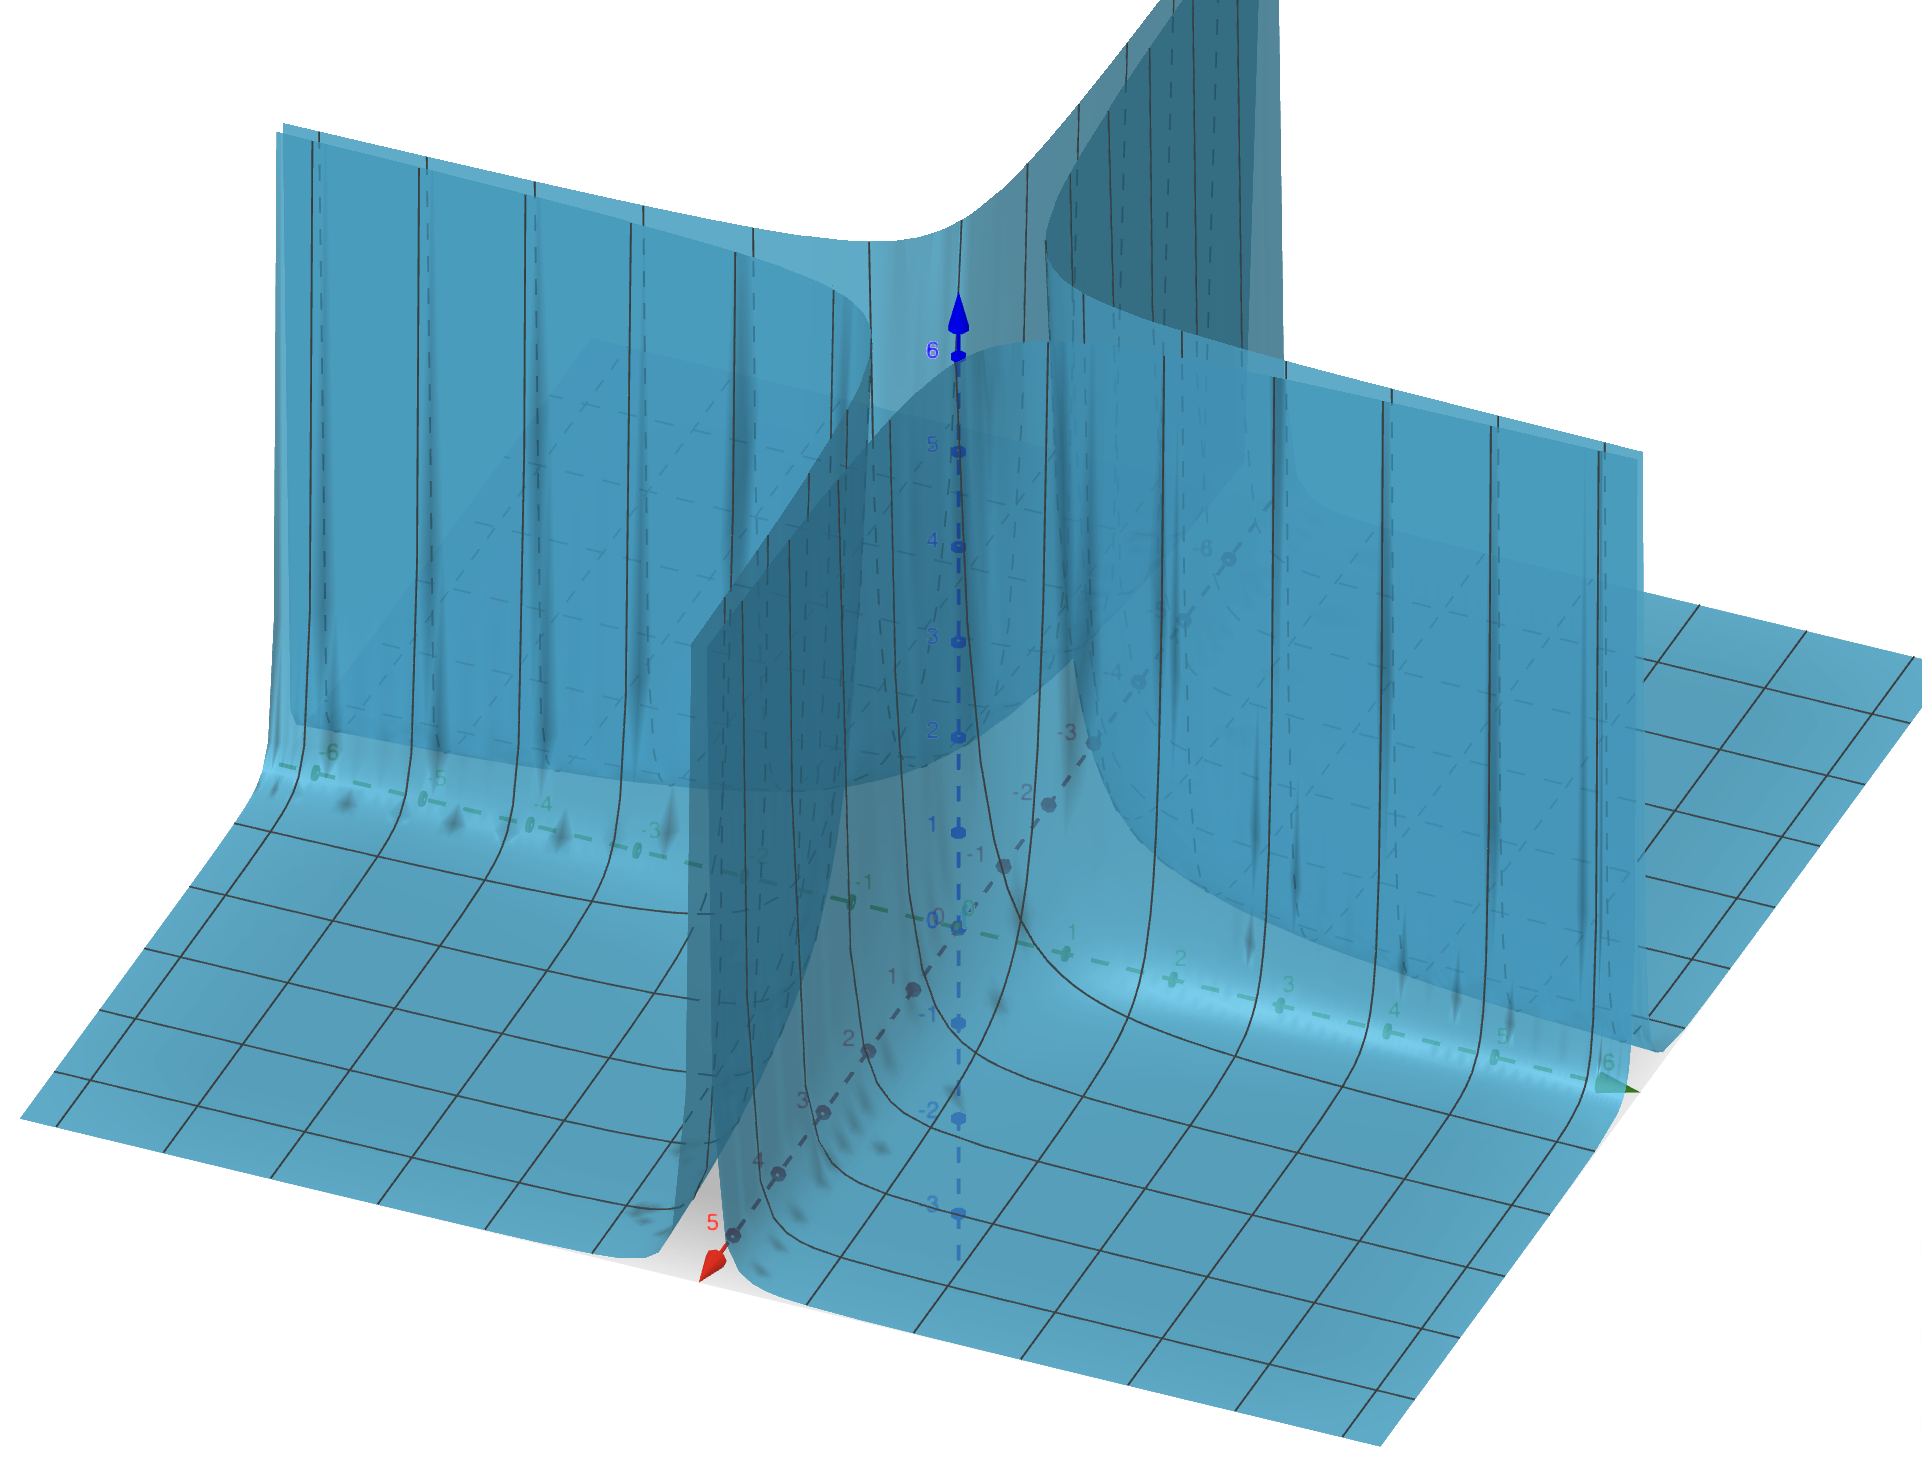
\includegraphics[scale=0.25]{images/Screenshot 2023-01-04 at 18.10.14.png}
        \caption{picture of $f(x,y)=\frac{1}{x^2y^2}$}
    \end{figure}
    \begin{enumerate}
        \item We can use theorem\ref{Equivalent definition of extended intrgral 1} to compute. Set $$C_N=[\frac{N+1}{N},N]^2$$
        Firstly, we need to show the sequence $\int_{C_N}|f|$ is bounded.
        \begin{equation}
            \begin{split}
                \int_{C_N}|f| &= \int_{C_N}f\\
                &= \int_{x\in[\frac{N+1}{N},N]}\int_{y\in[{\frac{N+1}{N},N}]}\frac{1}{x^2y^2}\di y\di x\\
                &= \int_{x\in[\frac{N+1}{N},N]}\left(\frac{-1}{x^2}\cdot \frac{1}{y}\right) \bigg\rvert_{\frac{N+1}{N}}^N\di x\\
                &= \int_{x\in[\frac{N+1}{N},N]}(\frac{N}{N+1}-\frac{1}{N})\frac{1}{x^2}\di x\\
                &= (\frac{N}{N+1}-\frac{1}{N})\frac{-1}{x} \bigg\rvert_{\frac{N+1}{N}}^N\\
                &= (\frac{N}{N+1}-\frac{1}{N})^2
            \end{split}
        \end{equation}
        Taking the limit we have $$\lim_{N\to\infty}(\frac{N}{N+1}-\frac{1}{N})^2=1$$
        So $f$ is integrable over $A$.
        \begin{equation}
            \begin{split}
                \int_Af &= \lim_{N\to\infty}\int_{C_N}f\\
                &= \lim_{N\to\infty}(\frac{N}{N+1}-\frac{1}{N})^2\\
                &= 1
            \end{split}
        \end{equation}
        \item It is easier for us to use theorem\ref{Equivalent definition of extended intrgral 2} to solve this problem.
        Set $$U_N=(1,N)^2$$
        Can check that $U_1\subset U_2\subset\cdots$ and $\bigcup_{N=1}^{\infty}U_N=A$. By theorem\ref{f integrable over S iff E has measure zero}, $E=Bd(\overline{U_N})$ has measure zero, so $f$ is integrable over $\overline{U_N}$.
        By theorem\ref{integral over interior}, $\int_{U_N}f=\int_{\overline{U_N}}f$.
        \begin{equation}
            \begin{split}
                \int_{U_N}|f| &= \int_{\overline{U_N}}f\\
                &= \int_{x\in[1,N]}\int_{y\in[1,N]}\frac{1}{x^2y^2}\di y\di x\\
                &= \int_{x\in[1,N]}(\frac{-1}{x^2}\cdot\frac{1}{y}) \bigg\rvert_1^N\di x\\
                &= \int_{x\in[1,N]}(1-\frac{1}{N})\frac{1}{x^2}\di x\\
                &= (1-\frac{1}{N})\frac{-1}{x} \bigg\rvert_1^N\\
                &= (1-\frac{1}{N})^2 
            \end{split}
        \end{equation}
        Taking the limit we have $$\lim_{N\to\infty}(1-\frac{1}{N})^2 =1$$
        So $f$ is integrable over $A$, and 
        \begin{equation}
            \begin{split}
                \int_Af &= \lim_{N\to\infty}\int_{U_N}f\\
                &= \lim_{N\to\infty}(1-\frac{1}{N})^2\\
                &= 1
            \end{split}
        \end{equation}
    \end{enumerate}
    \item Define the function $f$ and two sets $A$ and $B$ $$f(x,y)=\frac{1}{(y+1)^2}$$ $$A=\{(x,y):x>0\text{ and }x<y<2x\}$$ $$B=\{(x,y):x>0\text{ and }x^2<y<2x^2\}$$
    Show that $f$ is not integrable over $A$ but is integrable over $B$ and claculate it.
    \begin{figure}[ht]
        \centering
        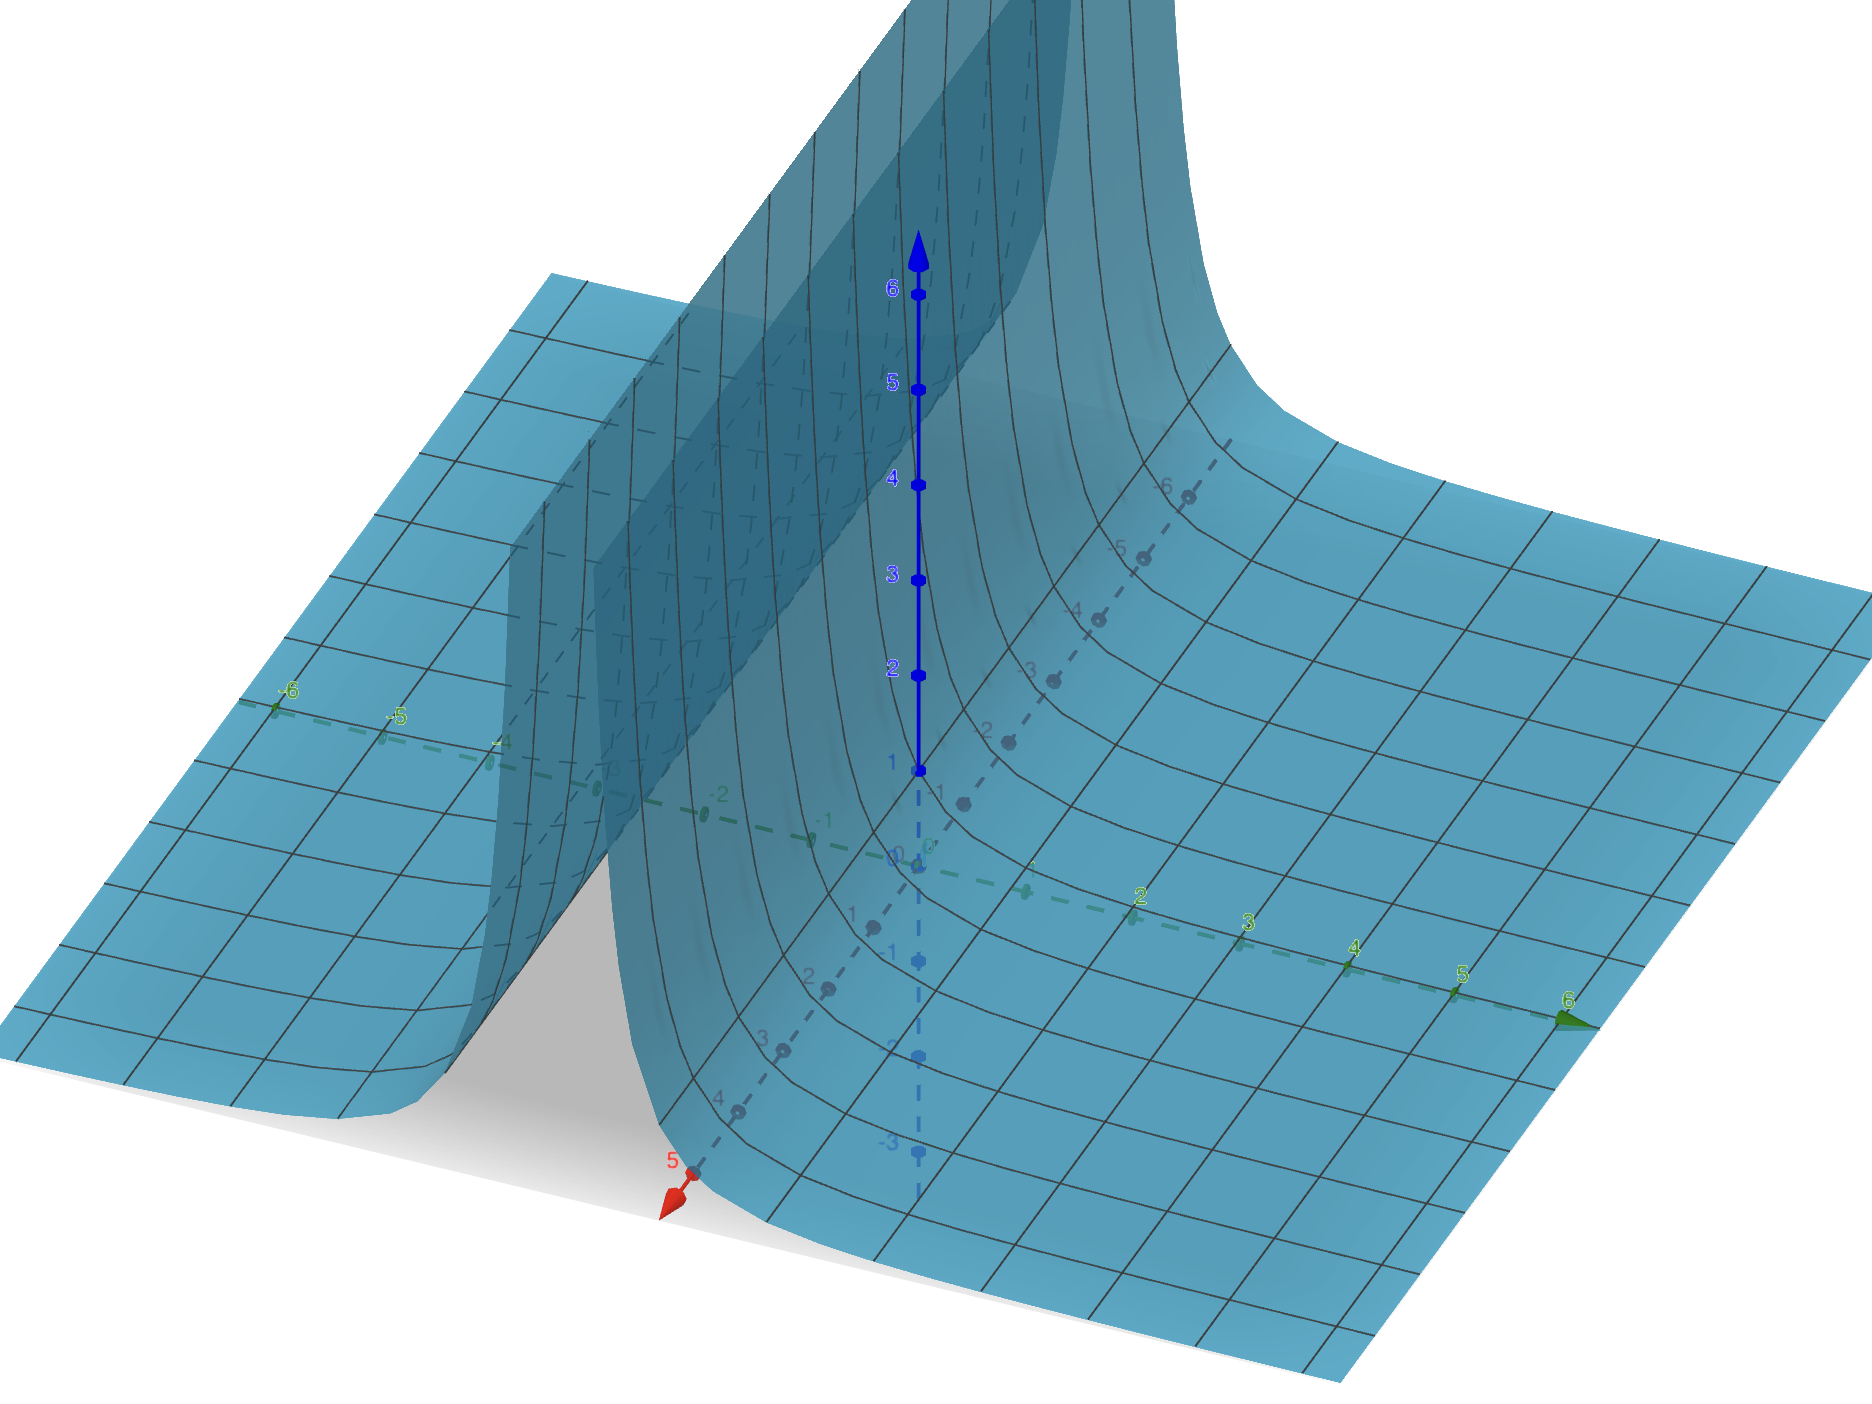
\includegraphics[scale=0.25]{images/Screenshot 2023-01-04 at 18.42.09.png}
        \caption{picture of $f(x,y)=\frac{1}{(y+1)^2}$}
    \end{figure}
    \begin{figure}[ht]
        \centering
        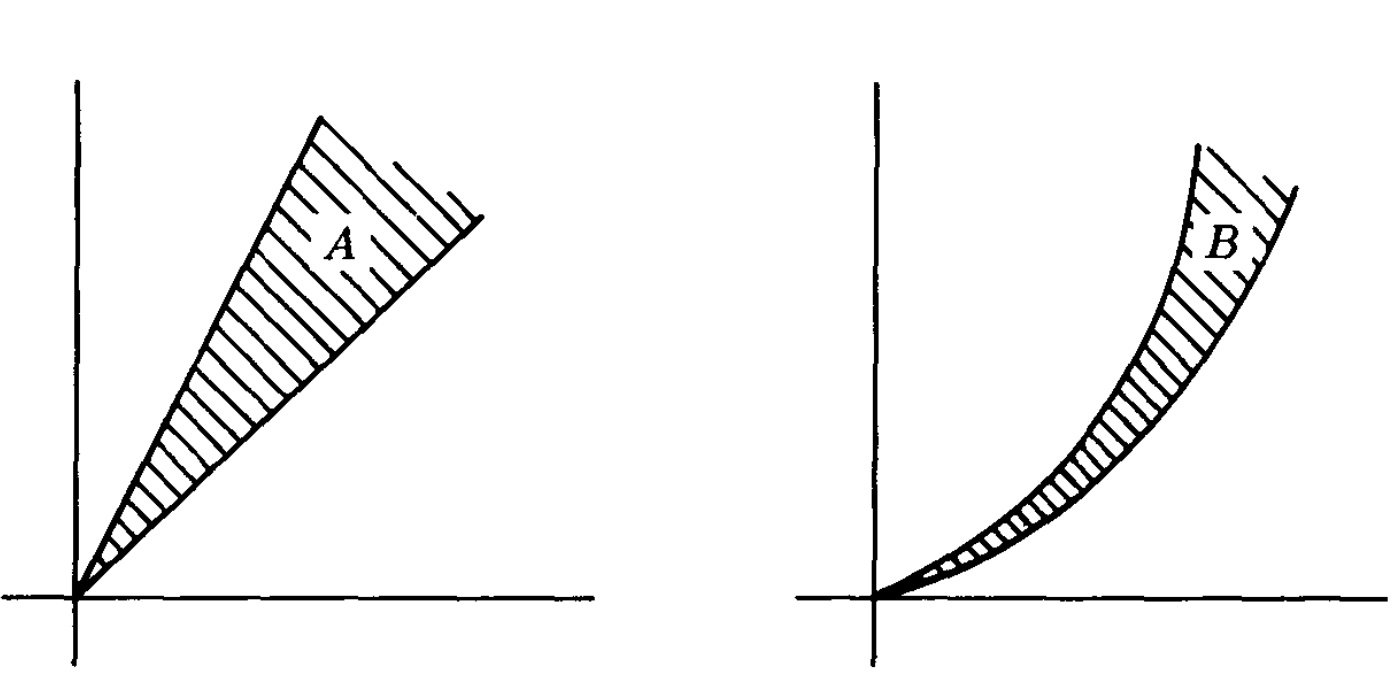
\includegraphics[scale=0.4]{images/Screenshot 2023-01-04 at 18.46.45.png}
        \caption{picture of $A,B$}
    \end{figure}
    \begin{enumerate}
        \item We show that $f$ is not integrable over $A$. Let $$U_N=\{(x,y):x\in(0,N)\text{ and }x< y< 2x\}$$
        With similar argument of the last example, we have 
        \begin{equation}
            \begin{split}
                \int_{U_N}|f| &= \int_{U_N}f\\
                &= \int_{\overline{U_N}}f\\
                &= \int_{x\in[0,N]}\int_{y=x}^{y=2x}\frac{1}{(y+1)^2}\di y\di x\\
                &= \int_{x\in[0,N]}(-\frac{1}{2x+1}+\frac{1}{x+1})\di x\\
                &= \log(N+1)
            \end{split}
        \end{equation}
        Taking the limit we have $$\lim_{N\to \infty}\log(N+1)=\infty$$
        So $f$ is not integrable over $A$.
        \item For the open set $B$, we set $$U_N=\{(x,y):x\in(0,N)\text{ and }x^2< y< 2x^2\}$$
        With similar argument of the last example, we have 
        \begin{equation}
            \begin{split}
                \int_{U_N}|f| &= \int_{U_N}f\\
                &= \int_{\overline{U_N}}f\\
                &= \int_{x\in[0,N]}\int_{y=x^2}^{y=2x^2}\frac{1}{(y+1)^2}\di y\di x\\
                &= \int_{x\in[0,N]}(-\frac{1}{2x^2+1}+\frac{1}{x^2+1})\di x\\
                &= \left(\arctan(x)-\frac{\arctan(\sqrt{2}x)}{\sqrt{2}}\right) \bigg\rvert_0^N\\
                &= \arctan(N)-\frac{\arctan(\sqrt{2}N)}{\sqrt{2}}
            \end{split}
        \end{equation}
        Taking the limit we have $$\lim_{N\to\infty}\arctan(N)-\frac{\arctan(\sqrt{2}N)}{\sqrt{2}}=\frac{\pi}{2}\left(1-\frac{1}{\sqrt{2}}\right)$$
        So $f$ is integrable over $B$.
        \begin{equation}
            \begin{split}
                \int_Bf &= \lim_{N\to\infty}\int_{U_N}f\\
                &= \lim_{N\to\infty}\arctan(N)-\frac{\arctan(\sqrt{2}N)}{\sqrt{2}}\\
                &=\frac{\pi}{2}\left(1-\frac{1}{\sqrt{2}}\right)
            \end{split}
        \end{equation}
    \end{enumerate}
\end{itemize}
\chapter{Change of Variables}

\section{Partitions of Unity}

\noindent \textbf{Motivation}:
\begin{itemize}
    \item In order to prove the change of variables theorem, we need a new equivalent definition of the extended integral.
    This definition of integral break the function $f$ up into functions $\phi_Nf$ where $\phi_N$ can be thought of some kind of proportion function, 
    each of which vanishes outside a compact set $S_N$ and we take the limit of the corresponding integrals $\int_Af_N$. It is hard to compute but has many advantages for theoretical purposes such as proving the change of variable theorem.
\end{itemize}

\begin{lemma}
    Let $Q$ be a rectangle in $\R^n$. There is a $C^{\infty}$ function $\phi:\R^n\longrightarrow\R$ such that 
    \begin{equation*}
        \begin{cases}
            \phi(x)>0\text{\quad}x\in Int(Q)\\
            \phi(x)=0\text{\quad otherwise}
        \end{cases}
    \end{equation*}
\end{lemma}

\begin{lemma}
    Let $\mathcal{A}$ be a collection of open sets in $\R^n$. Let $A$ be their union. Then there exists a countable collection $\{Q_1,Q_2,\cdots\}$ of rectangles contained in $A$ such that
    \begin{enumerate}
        \item The sets $Int(Q_i)$ cover $A$.
        \item Each $Q_i$ is contained in an element of $\mathcal{A}$.
        \item (Local finiteness) Each point of $A$ has a neighborhood that intersects only finitely many of the sets $Q_i$.
    \end{enumerate}
\end{lemma}

\begin{definition}
    If $\phi:\R^n\longrightarrow\R$, then the \underline{support} of $\phi$ is defined be the closure of the set $\{x:\phi(x)\neq0\}$.
\end{definition}

\begin{definition}
    Let $\mathcal{A}$ be a collection of open sets in $\R^n$. Let $A$ be their union. A collection of functions $\{\phi_i\}$ is said to be a \underline{partition of unity} on $A$ if it satisfies
    \begin{enumerate}
        \item $\forall x \in A.\phi_i(x)\geq 0$
        \item $S_i=supp(\phi_i)\subset A$
        \item $\forall a\in A.\exists\text{ open $U$ containing $a$ such that $U$ intersects only finitely of $S_i$}$.
        \item $\forall a \in A,\sum_{i=1}^{\infty}\phi_i(a)=1$
    \end{enumerate}
\end{definition}

\begin{theorem}[Existence of partition of unity]\label{existence of partition of unity}
    Let $\mathcal{A}$ be a collection of open sets in $\R^n$. Let $A$ be their union. 
    There exists a sequence $\{\phi_i\}$ of continuous functions $\phi_i:\R^n\longrightarrow\R$ such that
    \begin{enumerate}
        \item $\{\phi_i\}$ is a partition of unity.
        \item $\phi_i$ are of class $C^{\infty}$.
        \item $\{\phi_i\}$ has compact supports.
        \item $\forall i\in\N.S_i\text{ is contained in an element of }\mathcal{A}$.
    \end{enumerate}
\end{theorem}

\noindent\textbf{Example}:
\begin{itemize}
    \item Let $\phi_1:\R\longrightarrow\R$ be defined be the equation
    \begin{equation}
        \phi_1(x)=
        \begin{cases}
            \frac{1+\cos(x)}{2}\text{\quad}-\pi\leq x\leq \pi\\
            0\text{\quad otherwise}
        \end{cases}
    \end{equation}
    For each $m\in\N$, we set
    $$\phi_{2m+1}(x)=\phi_1(x-m\pi)$$
    $$\phi_{2m}(x)=\phi_1(x+m\pi)$$
    Can check that $\{\phi_i\}$ is a partition of unity of $\R$.
    \begin{figure}[ht]
        \centering
        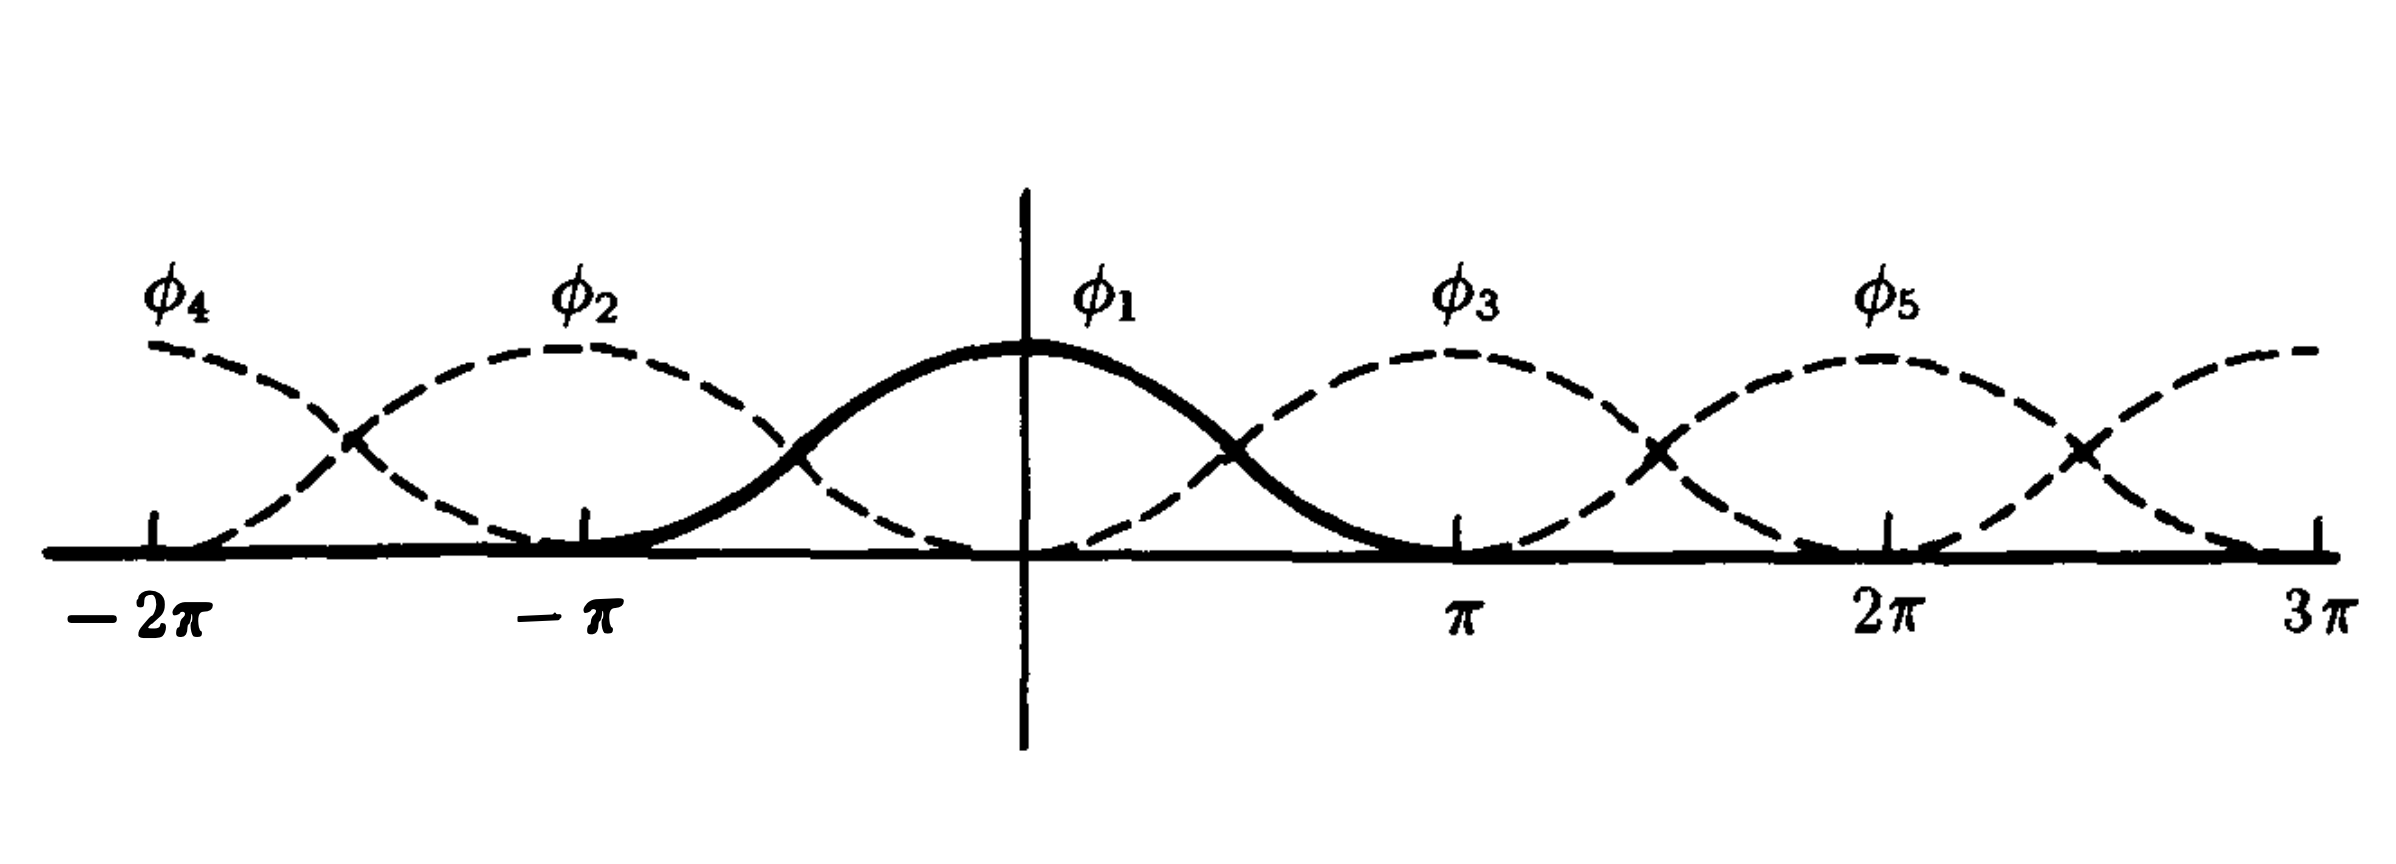
\includegraphics[scale=0.3]{images/Screenshot 2023-01-13 at 21.16.45.png}
        \caption{picture of $\{\phi_i\}$}
    \end{figure}
\end{itemize}

\begin{lemma}
    Let $A$ be opne in $\R^n$. Let $f:A\longrightarrow\R$ be continuous.
    If $f$ vanishes outside the compact subset $C$ of $A$, then the integral $\int_Af$ and $\int_Cf$ exist and are equal.
\end{lemma}

\begin{theorem}[Equivalent definition of extended intrgral 3]\label{Equivalent definition of extended intrgral 3}
    Let $A$ be opne in $\R^n$. Let $f:A\longrightarrow\R$ be continuous. Let $\{\phi_i\}$ be a partition of unity on $A$ having compact supports. The integral $\int_Af$ exists if and only if the series $\sum_{i=1}^{\infty}\int_A\phi_i|f|$ converges. Now
    $$\int_Af=\sum_{i=1}^{\infty}\int_A\phi_if$$
\end{theorem}

\section{Diffeomorphisms in $\R^n$}

\noindent\textbf{Motivation}:
In order to prove the change of variables theorem, we need to obtain two fundamental properties of diffeomorphisms. This we do in the present section.
\begin{itemize}
    \item The image of a compact rectifiable set under a diffeomorphism is another compact rectifiable set.
    \item Any diffeomorphism can be broken up locally into a composite of diffeomorphisms of a special type, called primitive diffeomorphisms.
\end{itemize}

\begin{definition}
    Let $A,B$ be open sets in $\R^n$. Let $g:A\longrightarrow B$ be bijective such that $g$ and $g^{-1}$ are of class $C^r$, then $g$ is called a \underline{diffeomorphism( of class $C^r$)}.
\end{definition}

\begin{lemma}
    Let $A$ be open in $\R^n$. Let $g:A\longrightarrow \R^n$ be a function of class $C^1$. 
    If the subset $E$ of $A$ has measure zero in $\R^n$, then the set $g(E)$ also has measure zero in $\R^n$.
\end{lemma}

\noindent\textbf{Remark}:
\begin{itemize}
    \item Differentiability is needed for the lemma above. If $g$ is merely conntinuous, then the image of a set of measure zero may not have measure zero. Consider the \underline{Peano space-filling curve} $f:[0,1]\longrightarrow[0,1]^2$.
\end{itemize}

\begin{theorem}
    Let $g:A\longrightarrow B$ be a diffeomorphism of class $C^r$, where $A,B$ are open in $\R^n$. Let $D$ be a compact subset of $A$.
    \begin{enumerate}
        \item $g(Int(D))=Int(g(D))\text{ and }g(Bd(D))=Bd(g(D))$
        \item If $D$ is rectifiable, then $g(D)$ is also rectifiable.
    \end{enumerate}
\end{theorem}

\begin{definition}
    Let $h:A\subset \R^n\longrightarrow B\subset \R^n$. Consider the component functions $$h(x)=(h_1(x),\cdots,h_n(x))$$
    We say $h$ is a \underline{primitive diffeomorphism} if $h$ preserves the i-th coordinate for some i.($h_i(x)=x_i$)
\end{definition}

\begin{theorem}
    Let $g:A\longrightarrow B$ be a diffeomorphism of open sets in $\R^n$. Given $a\in A$, there is a neighborhood $U_0$ of $a$ contained in $A$, and a sequence of diffeomorphisms of open sets in $\R^n$
    \begin{equation*}
        \xymatrix{U_0 \ar[r]^{h_1} &U_1 \ar[r]^{h_2} &U_2 \ar[r]^{h_3} & \cdots \ar[r]^{h_k}&U_k} 
    \end{equation*}
    such that the composite $h_k\circ\cdots\circ h_2\circ h_1=g|_{U_0}$ and each $h_i$ is a primitive diffeomorphism.
\end{theorem}

\begin{lemma}
    Let $g:A\longrightarrow B$ be a diffeomorphism of open sets in $\R^n$. Then for every continuous function $f:B\longrightarrow \R$ that is integrable over $B$,
    the function $(f\circ g)|\det(Dg)|$ is integrable over $A$ and
    \begin{equation*}
        \int_Bf=\int_A(f\circ g)|\det(Dg)|
    \end{equation*}
\end{lemma}

\begin{lemma}
    Let $g:A\longrightarrow B$ be a diffeomorphism of open sets in $\R^n$. Let $f:B\longrightarrow \R$ be continuous. 
    If $(f \circ g)|\det(Dg)|$ is integrable over $A$, then $f$ is integrable over $B$.
\end{lemma}

\section{The Change of Variable Theorem}

\begin{theorem}[Substitution rule]
    Let $I=[a,b]$. Let $g:I\longrightarrow\R$ be a function of class $C^1$ with $g'(x)\neq0$ for $x\in(a,b)$.
    Then the set $g(I)$ is a closed interval $J$ with end points $g(a)$ and $g(b)$.
    If $f:J\longrightarrow\R$ is continuous, then $$\int_{g(a)}^{g(b)}f=\int_a^b(f\circ g)g'$$
\end{theorem}

\begin{definition}
    Let $A$ be open in $\R^n$. Let $g:A\longrightarrow\R^n$ be a injective function of class $C^r$, such that $$\forall x\in A.\det(Dg(x))\neq0$$
    Then $g$ is called a \underline{change of variables} in $\R^n$.
\end{definition}

\begin{theorem}
    $g$ is a change of variables in $\R^n$ if and only if $g$ is a diffeomorphism in $\R^n$.
\end{theorem}

\begin{theorem}[Change of variables theorem]\label{Change of variables theorem}
    Let $g:A\longrightarrow B$ be a diffeomorphism of open sets in $\R^n$. Let $f:B\longrightarrow \R$ be a continuous function. 
    Then $f$ is integrable over $B$ if and only if $(f\circ g)\cdot |\det(Dg)|$ is integrable over $A$. In this case 
    $$\int_Bf=\int_A(f\circ g)\cdot |\det(Dg)|$$
\end{theorem}

\section{Applications}

\subsection{Polar, Spherical and Cylindrical Coordinate}

\begin{definition}
    The \underline{polar coordinate transformation} is a function $g:\R^2\longrightarrow\R^2$ defined by 
    $$g(r,\theta)=(r\cos\theta,r\sin\theta)$$
    By computation we have
    \begin{equation*}
        \det(Dg)=\det(\begin{bmatrix}
            D_1g_1 & D_2g_1\\
            D_1g_2 & D_2g_2
        \end{bmatrix})=\det(\begin{bmatrix}
            \cos\theta & -r\sin\theta\\
            \sin\theta & r\sin\theta
        \end{bmatrix})=r(\cos^2\theta+\sin^2\theta)=r
    \end{equation*}
    \begin{figure}[H]
        \centering
        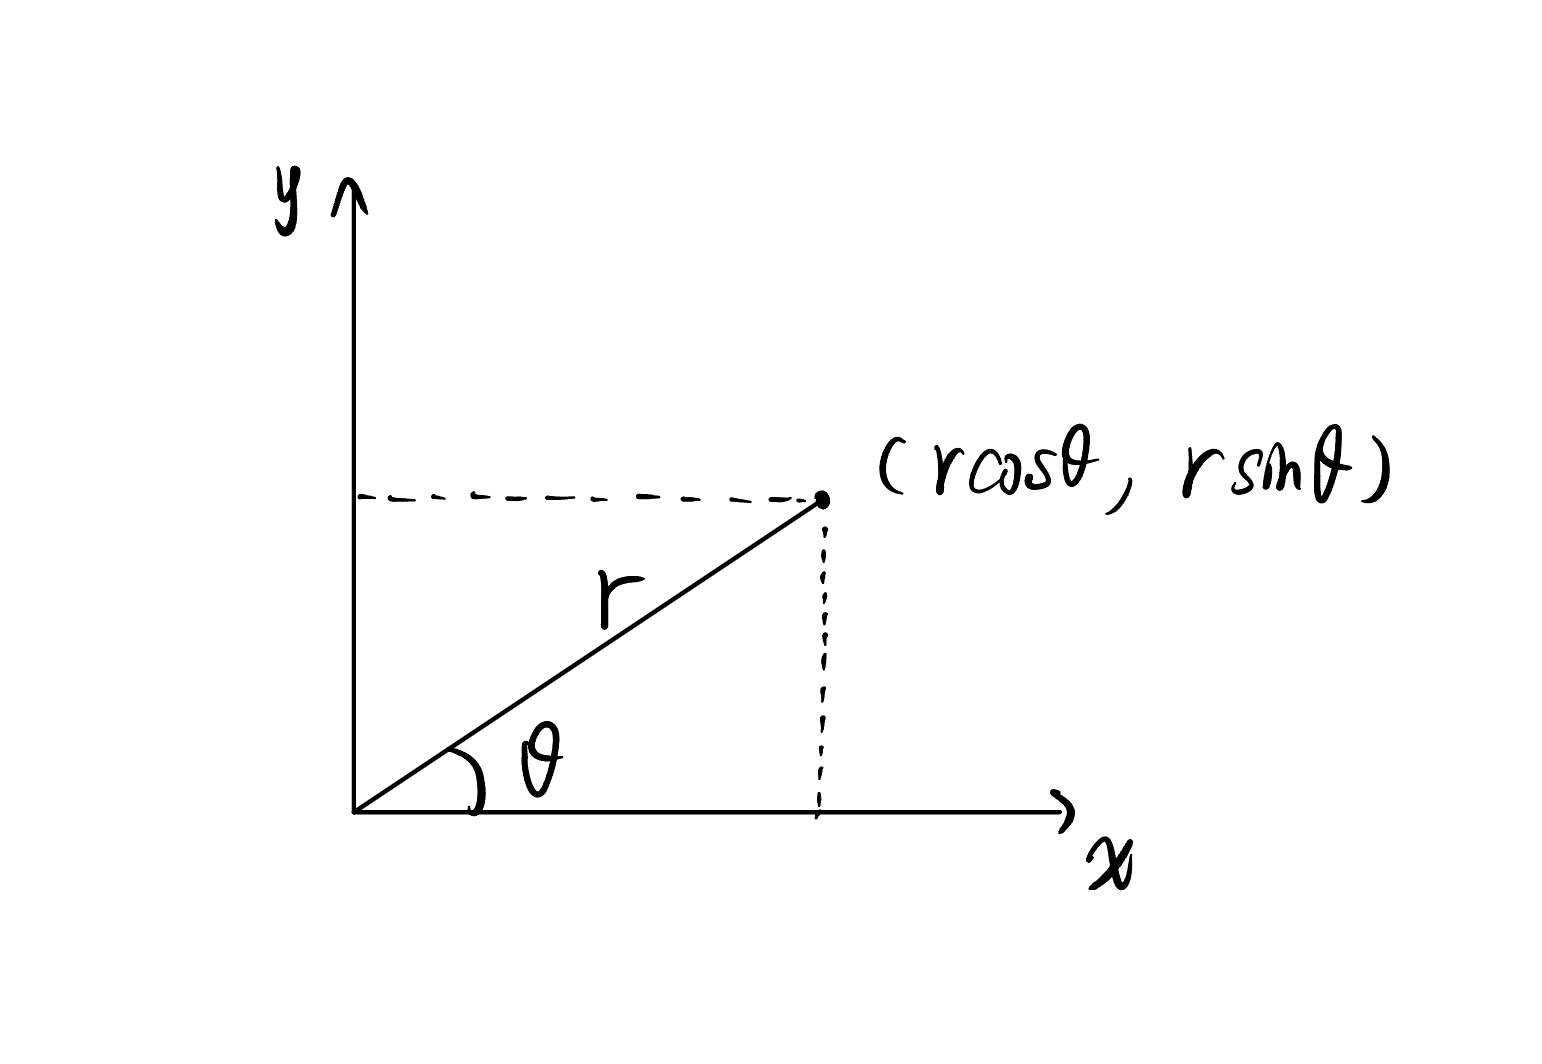
\includegraphics[scale=0.15]{images/IMG_0361.jpg}
        \caption{picture of polar coordinate}
    \end{figure}
\end{definition}
\noindent\textbf{Example}:
\begin{itemize}
    \item Let $B$ be the open set in $\R^2$ defined by $$B=\{(x,y):x>0\text{ and }y>0\text{ and }x^2+y^2<a^2\}$$
    One commonly computes an integral over $B$.i.e. $\int_Bf$ by using the polar coordinate transformation.
    Define the sets $A$ as 
    $$A=\{(r,\theta):0<r<a\text{ and }0<\theta<\frac{\pi}{2}\}$$
    The map $g:A\longrightarrow B$ is a diffeomorphism. The change of variables theorem implies that $$\int_Bf=\int_Af(r\cos\theta,r\sin\theta)\cdot r$$
    \begin{figure}[H]
        \centering
        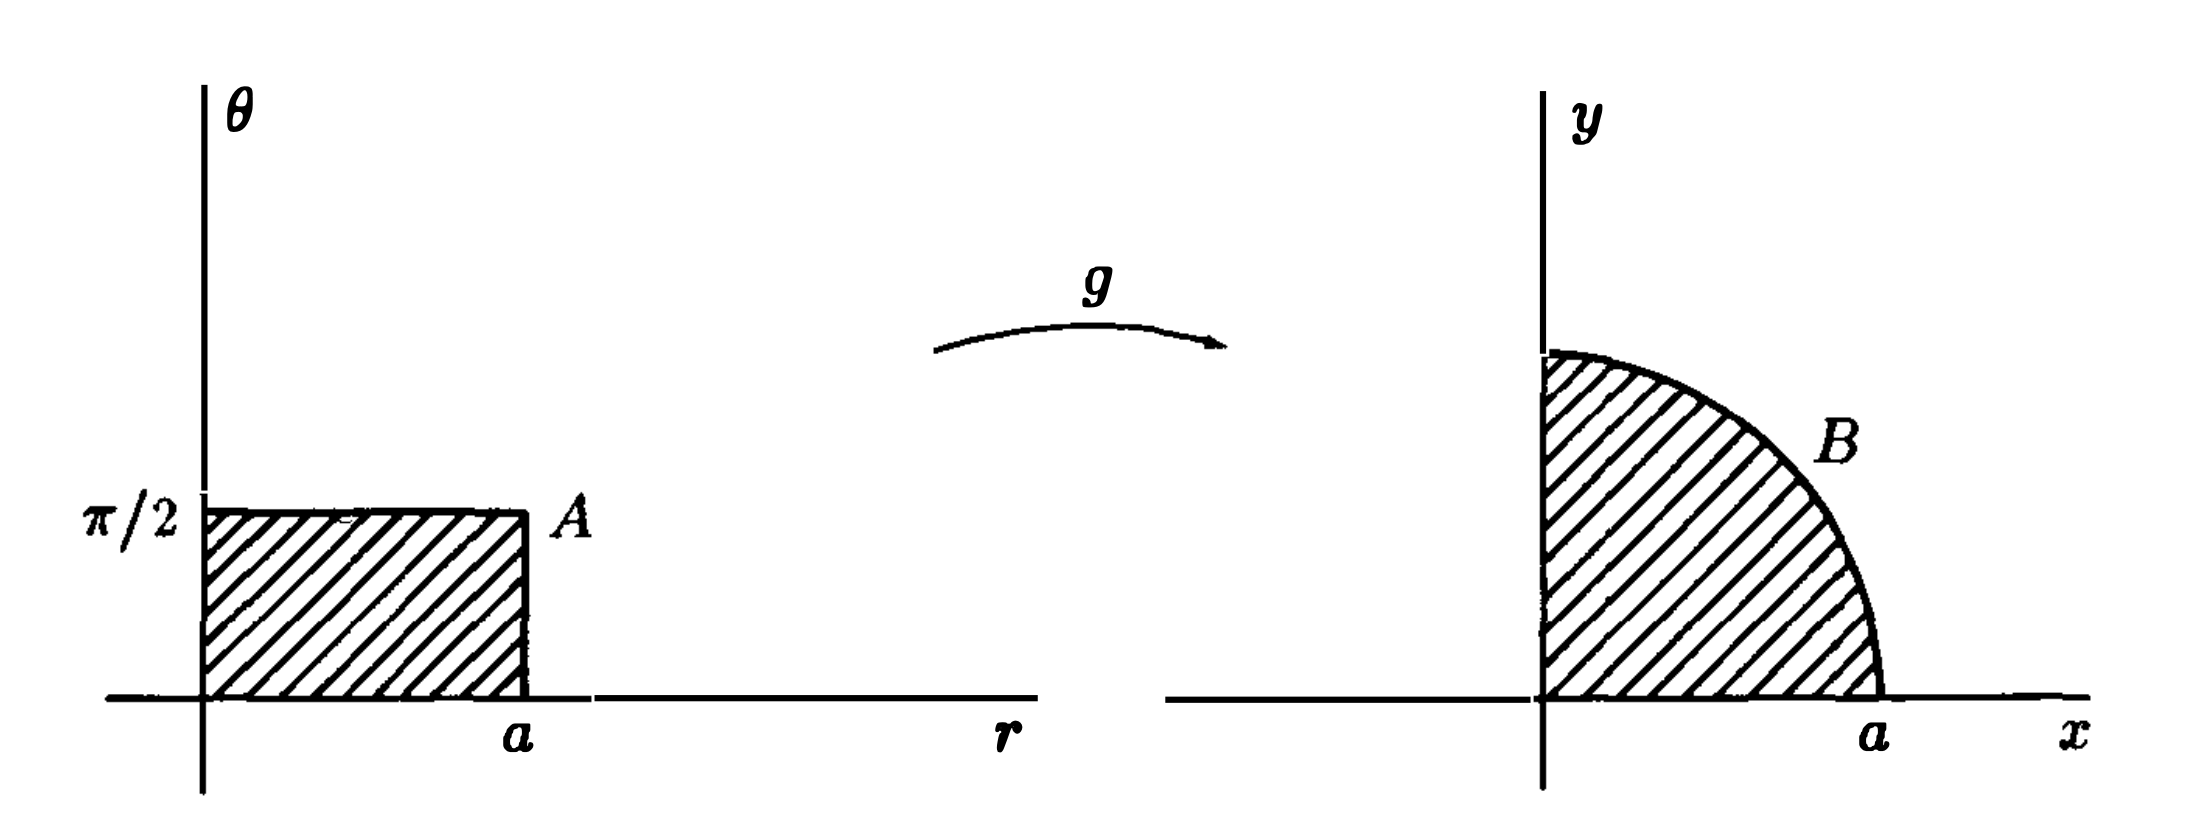
\includegraphics[scale=0.33]{images/Screenshot 2023-01-13 at 22.13.08.png}
        \caption{picture of polar coordinate transformation $g:A\to B$}
    \end{figure}
    \item If we want to integrate the function $f$ over the set
    $$W=\{(x,y):x^2+y^2<a^2\}$$
    The polar coordinate transformation cannot be a diffeomorphism now because the part where $y=0$ and $x>0$ cannot be bijective.
    However,we can define a diffeomorphism of the open $U=(0,a)\times(0,2\pi)$ with the open set $$V=\{(x,y): x^2+y^2<a^2\text{ and }x<0\text{ if }y=0\}$$
    Therefore, the integral can be evaluated as $$\int_Wf=\int_Vf=\int_Uf(r\cos\theta,r\sin\theta)\cdot r$$
    \begin{figure}[H]
        \centering
        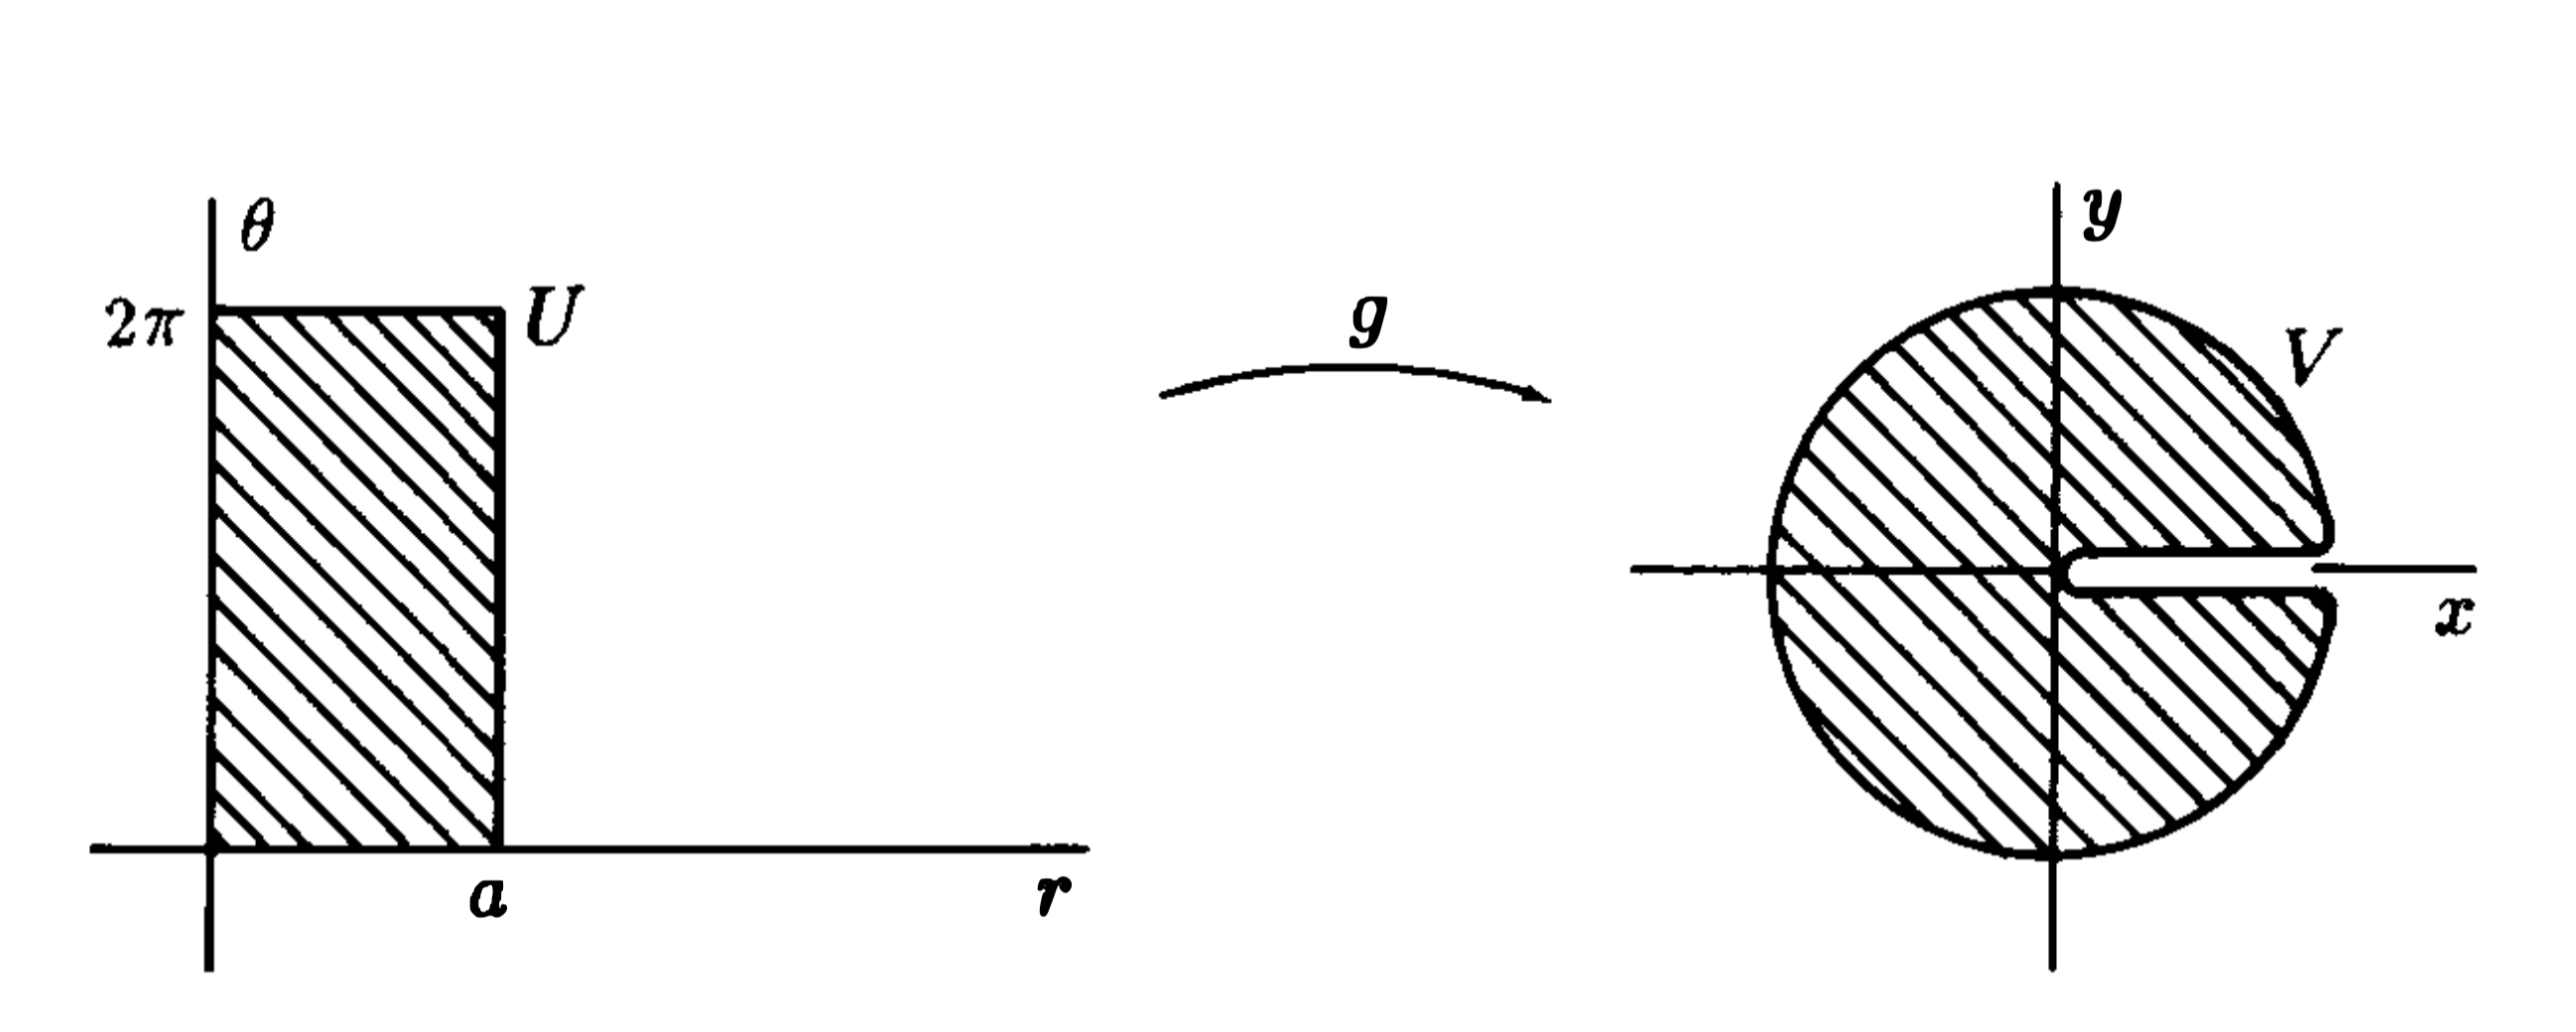
\includegraphics[scale=0.3]{images/Screenshot 2023-01-13 at 22.24.55.png}
        \caption{picture of polar coordinate transformation $g:U\to V$}
    \end{figure}
\end{itemize}


\begin{definition}
    The \underline{spherical coordinate transformation} is a function $g:\R^3\longrightarrow\R^3$ defined by 
    $$g(\rho,\phi,\theta)=(\rho\sin\phi\cos\theta,\rho\sin\phi\sin\theta,\rho\cos\phi)$$
    By computation we have
    \begin{equation*}
        \det(Dg)=\det(\begin{bmatrix}
            \sin\phi\cos\theta & \rho\cos\phi\cos\theta & -\rho\sin\phi\sin\theta\\
            \sin\phi\sin\theta & \rho\cos\phi\sin\theta & \rho\sin\phi\cos\theta\\
            \cos\phi & -\rho\sin\phi & 0
        \end{bmatrix})=\rho^2\cdot \sin\phi
    \end{equation*}
    \begin{figure}[H]
        \centering
        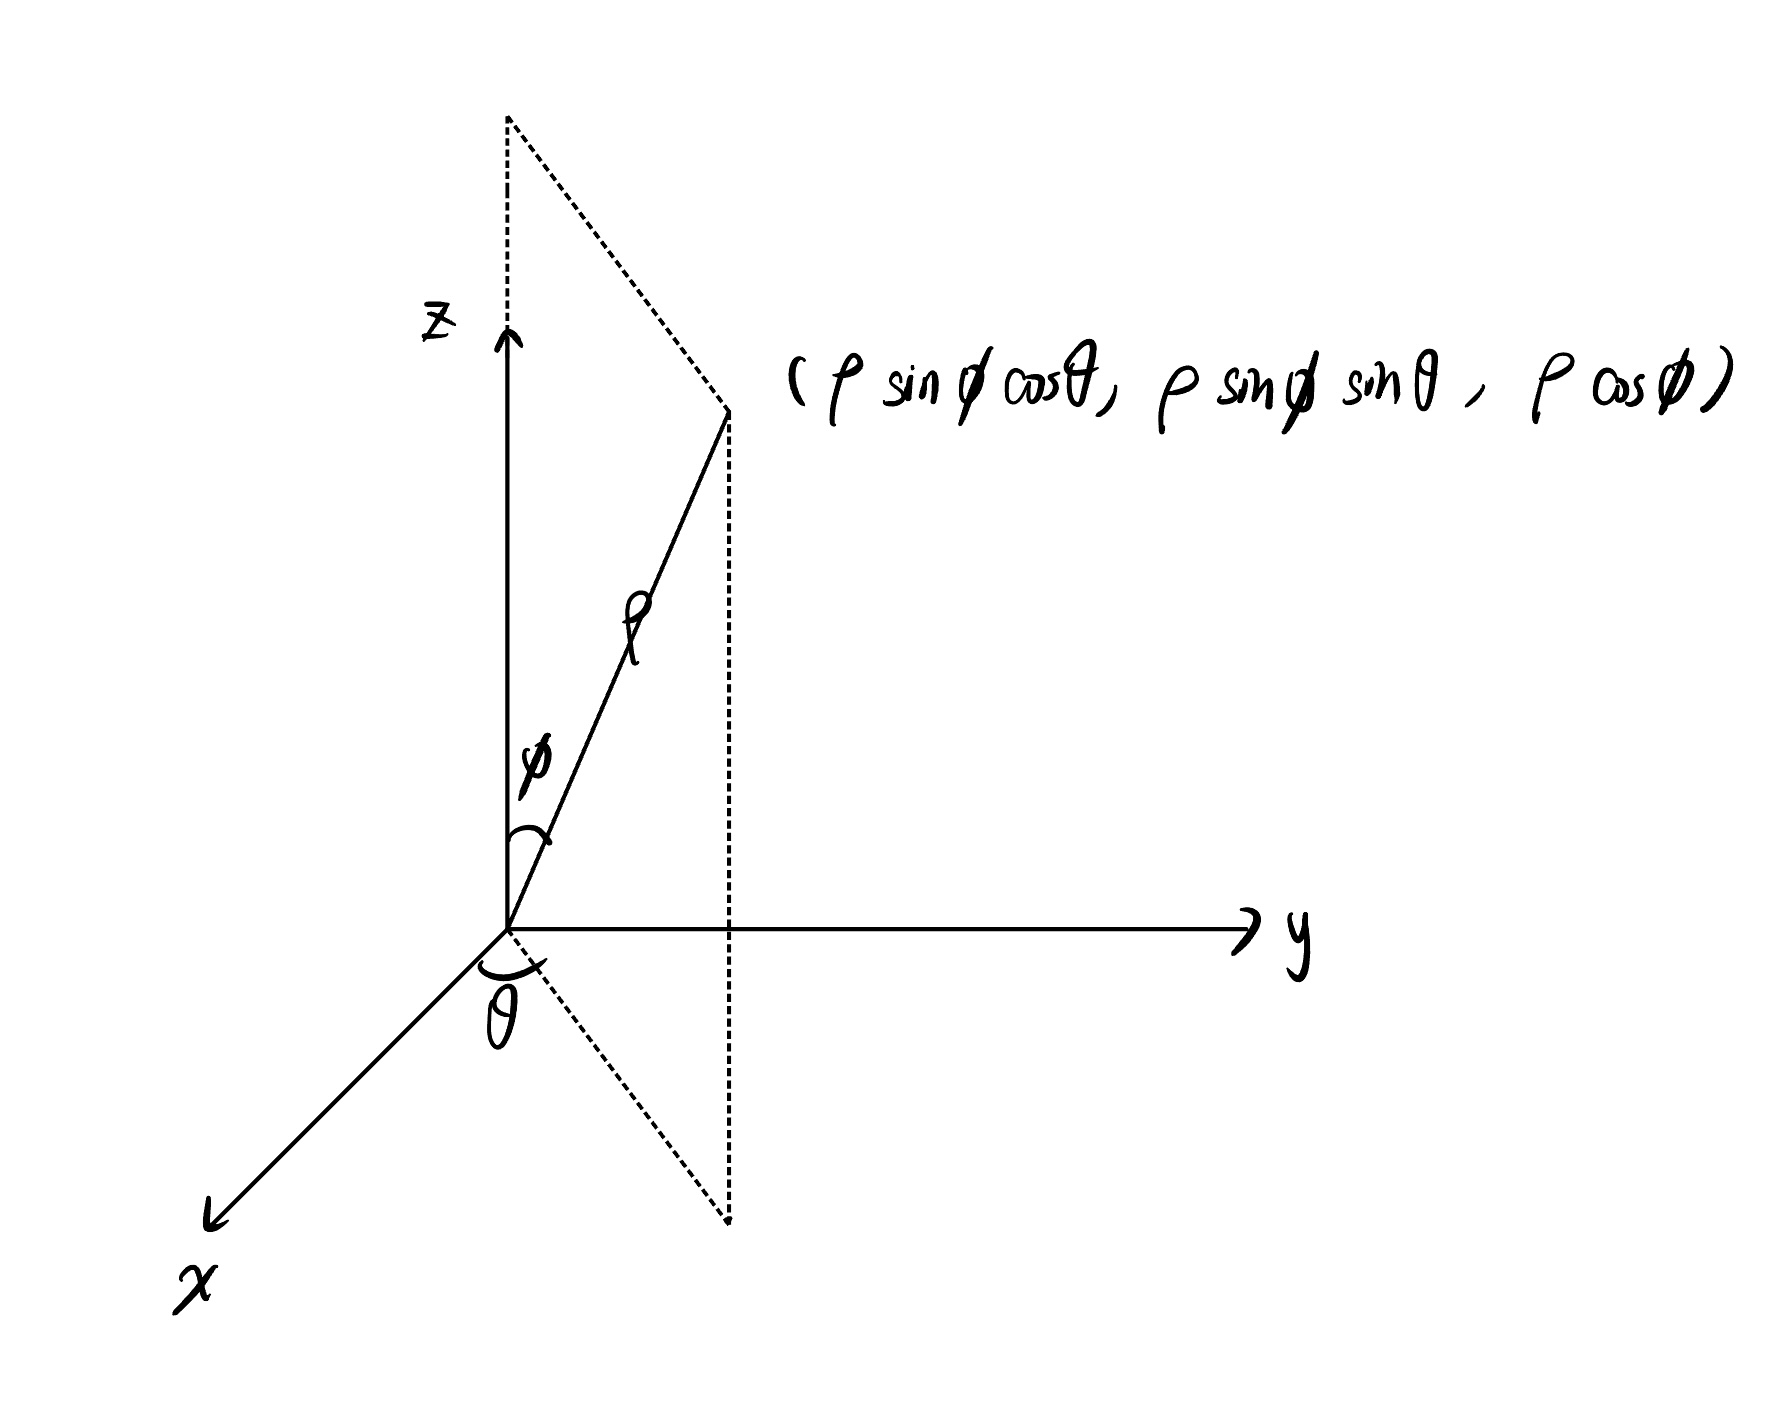
\includegraphics[scale=0.16]{images/IMG_0362.jpg}
        \caption{picture of spherical coordinate}
    \end{figure}
\end{definition}
\noindent\textbf{Example}:
\begin{itemize}
    \item Let $B$ be the open set in $\R^3$ defined by $$B=\{(x,y,z):x>0\text{ and }y>0\text{ and }x^2+y^2+z^2<a^2\}$$
    One commonly computes an integral over $B$.i.e. $\int_Bf$ by using the spherical coordinate transformation.
    Define the sets $A$ as 
    $$A=\{(\rho,\phi,\theta):0<\rho<a\text{ and }0<\phi<\pi\text{ and }0<\theta<\frac{\pi}{2}\}$$
    The map $g:A\longrightarrow B$ is a diffeomorphism. The change of variables theorem implies that $$\int_B=\int_Af(\rho\sin\phi\cos\theta,\rho\sin\phi\sin\theta,\rho\cos\phi)\cdot \rho^2\sin\phi$$
    \begin{figure}[H]
        \centering
        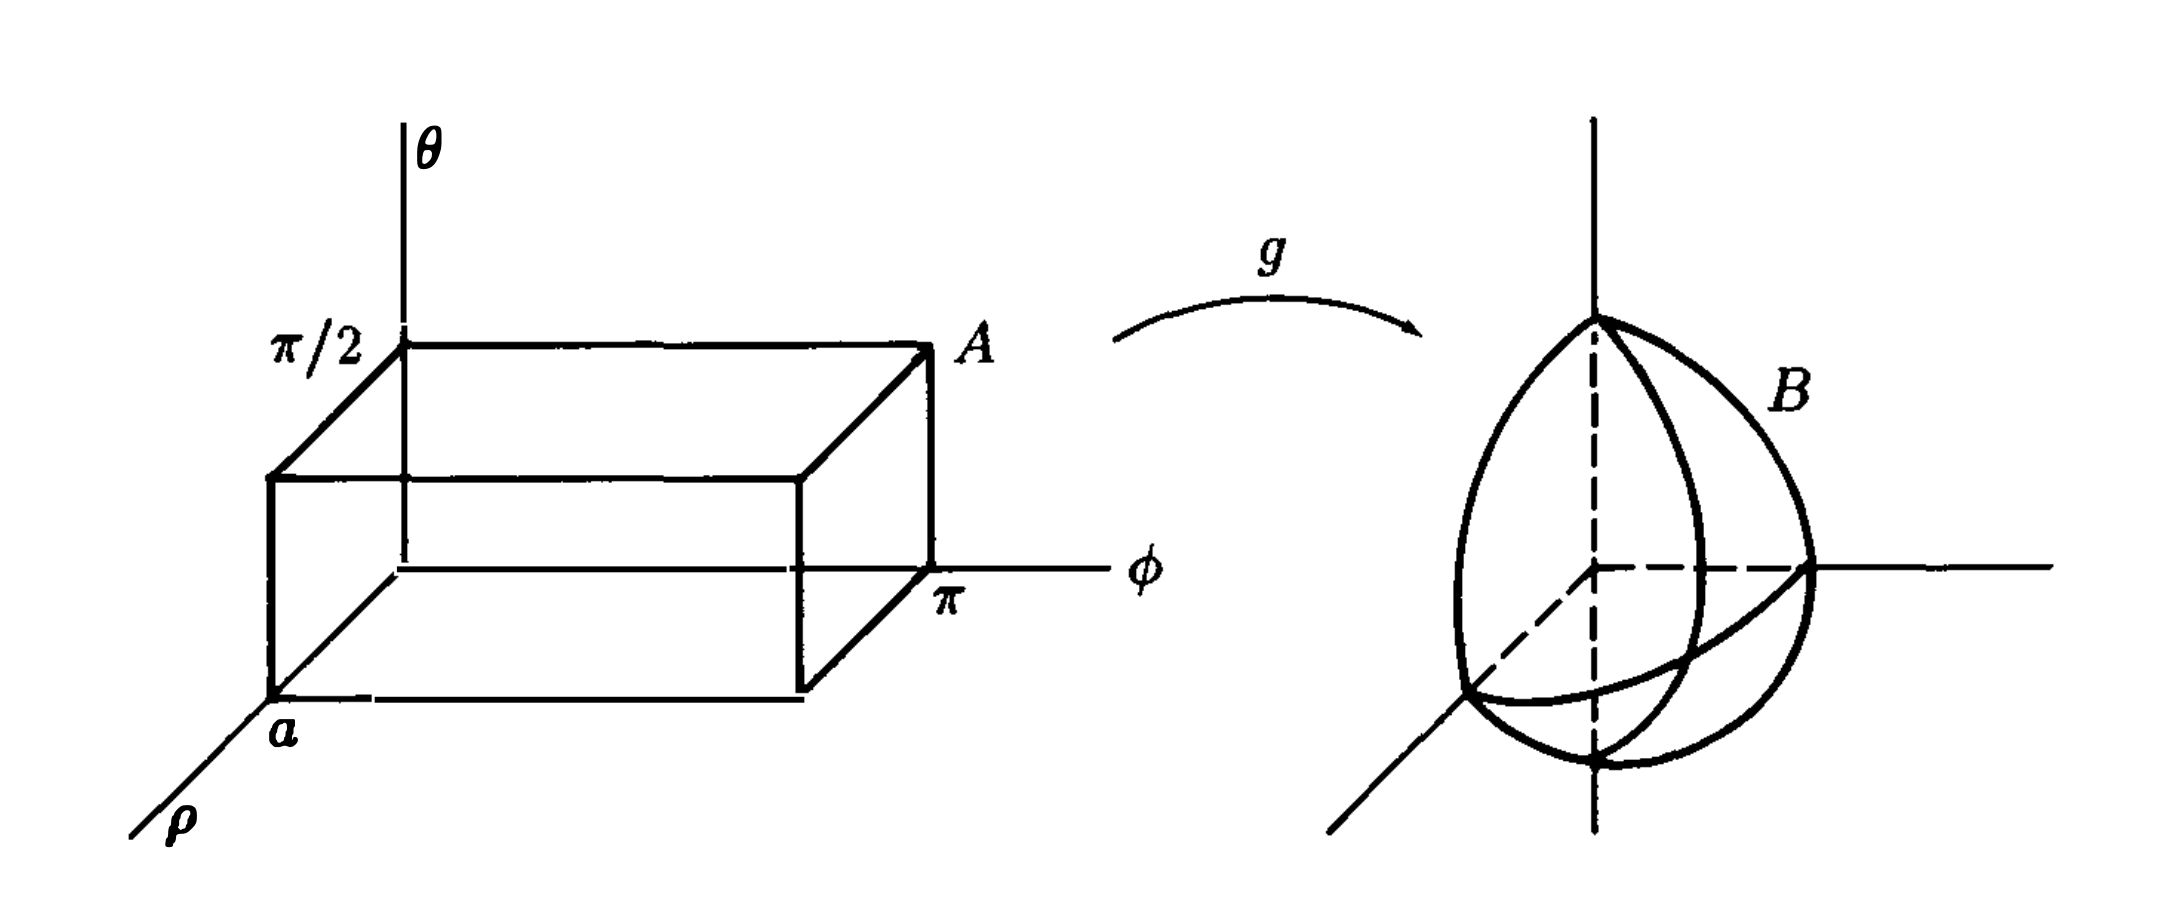
\includegraphics[scale=0.33]{images/Screenshot 2023-01-15 at 18.05.53.png}
        \caption{picture of spherical coordinate transformation $g:A\to B$}
    \end{figure}
\end{itemize}

\begin{definition}
    The \underline{Cylindrical coordinate transformation} is a function $g:\R^3\longrightarrow\R^3$ defined by
    $$g(r,\theta,z)=(r\cos\theta,r\sin\theta,z)$$
    By computation we have
    \begin{equation*}
        \det(Dg)=\det(\begin{bmatrix}
            \cos\theta & -r\sin\theta & 0\\
            \sin\theta & r\cos\theta & 0\\
            0 & 0 & 1
        \end{bmatrix})=r
    \end{equation*}
    \begin{figure}[H]
        \centering
        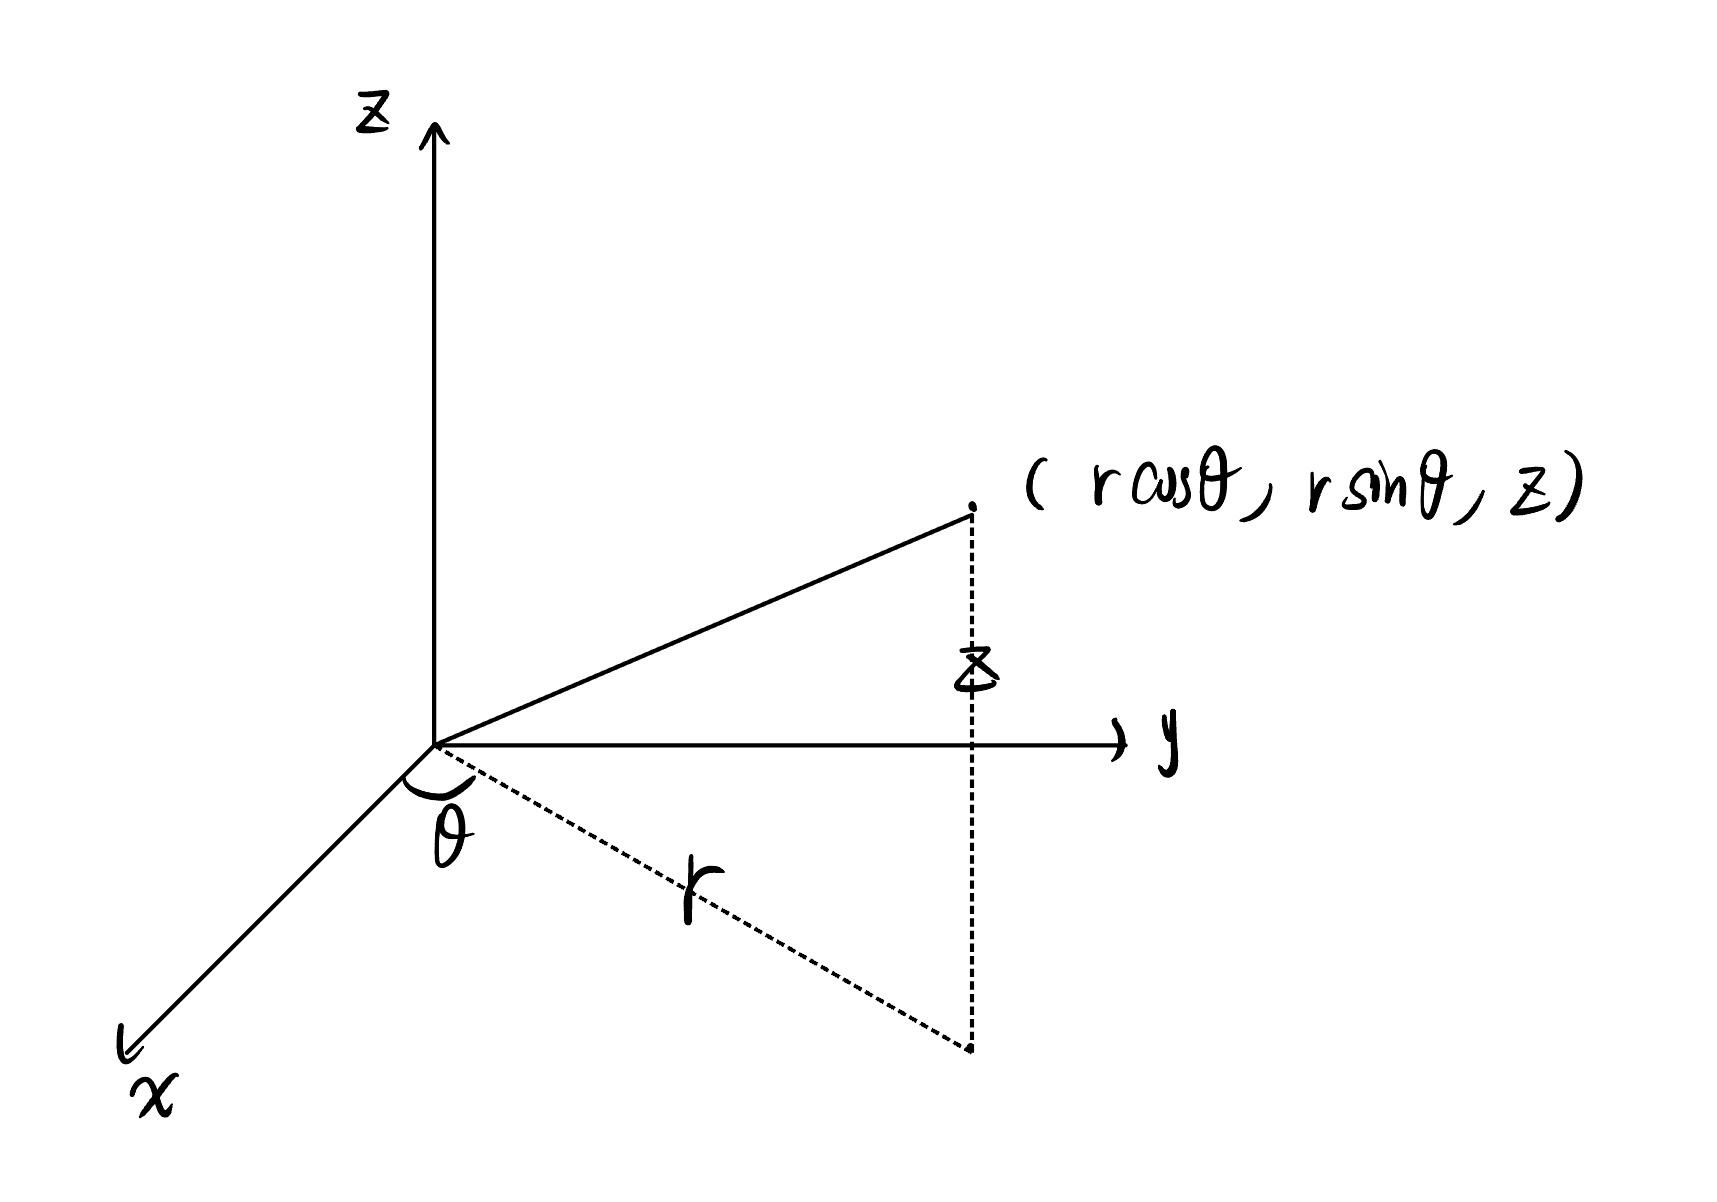
\includegraphics[scale=0.16]{images/IMG_0363.jpg}
        \caption{picture of cylindrical coordinate}
    \end{figure}
\end{definition}
\noindent\textbf{Example}:
\begin{itemize}
    \item We can use cylindrical coordinate transformation to compute the volume of a solid torus.
    Let $g$ be the cylindrical coordinate transformation. Let $$A=\{(r,\theta,z):(r-b)^2+z^2\leq a^2\text{ and }0\leq \theta\leq 2\pi\}$$
    The \underline{Solid Torus} $T$ is the image of $A$ under $g$. The volume of $T$ , say $V$, is $\int_T1$.
    \begin{figure}[H]
        \centering
        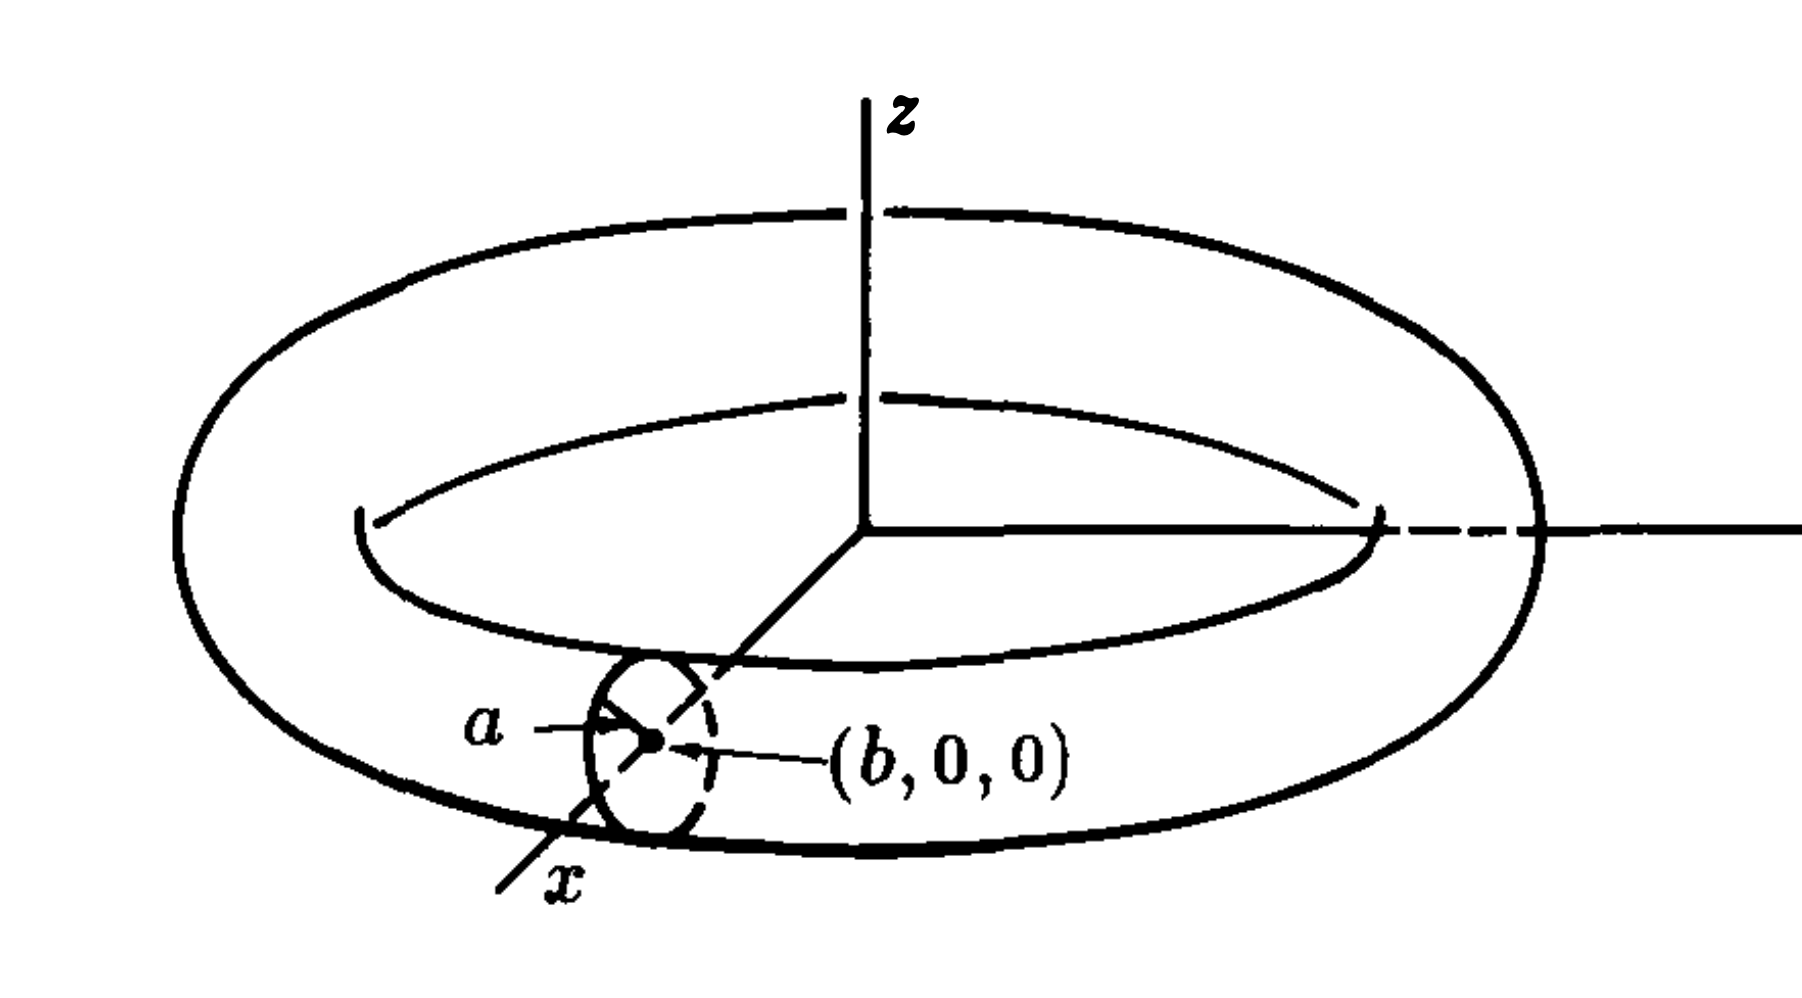
\includegraphics[scale=0.35]{images/Screenshot 2023-02-07 at 17.58.09.png}
        \caption{A solid torus in $\R^3$.}
    \end{figure}
    $$Int(A)=\{(r,\theta,z):(r-b)^2+z^2< a^2\text{ and }0< \theta< 2\pi\}$$
    Define $$T'=Int(T)\setminus\{(x,y,x)\in T: y=0 \text{ and }x>0\}$$
    Now $g:Int(A)\longrightarrow T'$ is a diffeomorphism, so we can apply the change of variable theorem.
    \begin{equation*}
        \int_{T'}1=\int_{Int(A)}(1\circ g)\cdot r
    \end{equation*}
    Since $Bd(A)$ and $Bd(T)\cup\{(x,y,x)\in T: y=0 \text{ and }x>0\}$ both have measure zero in $\R^3$ because by basic topology, their dimensions are both 2, which is less than 3.
    Therefore
    \begin{equation*}
        \begin{split}
            V &= \int_T1\\
            &=\int_{T'}1\\
            &= \int_{Int(A)}(1\circ g)\cdot r\\
            &= \int_{A}(1\circ g)\cdot r\\
            &= \int_Ah\text{\quad where }h(r,\theta,z)=r\\
            &= \int_Qh_A\text{\quad where }A\subset Q=[b-a,b+a]\times[0,2\pi]\times[-a,a]\\
            &= \int_{r=b-a}^{r=b+a}\int_{\theta=0}^{\theta=2\pi}\int_{z=-a}^{z=a}h_A\di z \di \theta \di r\\
            &=\int_{r=b-a}^{r=b+a}\int_{\theta=0}^{\theta=2\pi}2\sqrt{a^2-(r-b)^2}\cdot r \di \theta\di r\\
            &=\int_{r=b-a}^{r=b+a}4\pi\cdot r \cdot \sqrt{a^2-(r-b)^2}\di r\\
            &=2\pi^2a^2b
        \end{split}
    \end{equation*}
\end{itemize}

\subsection{n-dimensional Cone, Ball in $\R^n$}

\begin{definition}
    Given a rectifiable set $S$ in $\R^n$. We define the \underline{centroid} of $S$ to be the point $c(S)\in \R^n$ such that
    for each $k\in\{1,\cdots,n\}$ $$c_k(S)=\frac{1}{v(S)}\int_S\pi_k$$ where $\pi_k$ is the projection function.
\end{definition}

\begin{definition}
    We say $S$ is \underline{symmetric} with respect to the subspace $x_k=0$ of $\R^n$ if the transformation $$h(x)=(x_1,\cdots,x_{k-1},-x_k,x_{k+1},\cdots,x_n)$$ carries $S$ onto itself.
\end{definition}

\begin{theorem}
    If $S$ is symmetric with respect to the subspace $x_k=0$ of $\R^n$, then $c_k(S)=0$.
\end{theorem}

\begin{definition}
    Let $A$ be an open rectifiable set in $\R^{n-1}$. Given the point $p\in\R^n$ with $p_n>0$. 
    Define $$S=\{x\in\R^n:x=(1-t)a+tp\text{ where }a\in A\times0\text{ and }0<t<1\}$$
    Then $S$ is the union of all open line segments in $\R^n$ joining $p$ to points of $A|times0$. The closure of $S$ is called the \underline{cone} with base $\overline{A}\times0$ and vertex $p$.
    \begin{figure}[H]
        \centering
        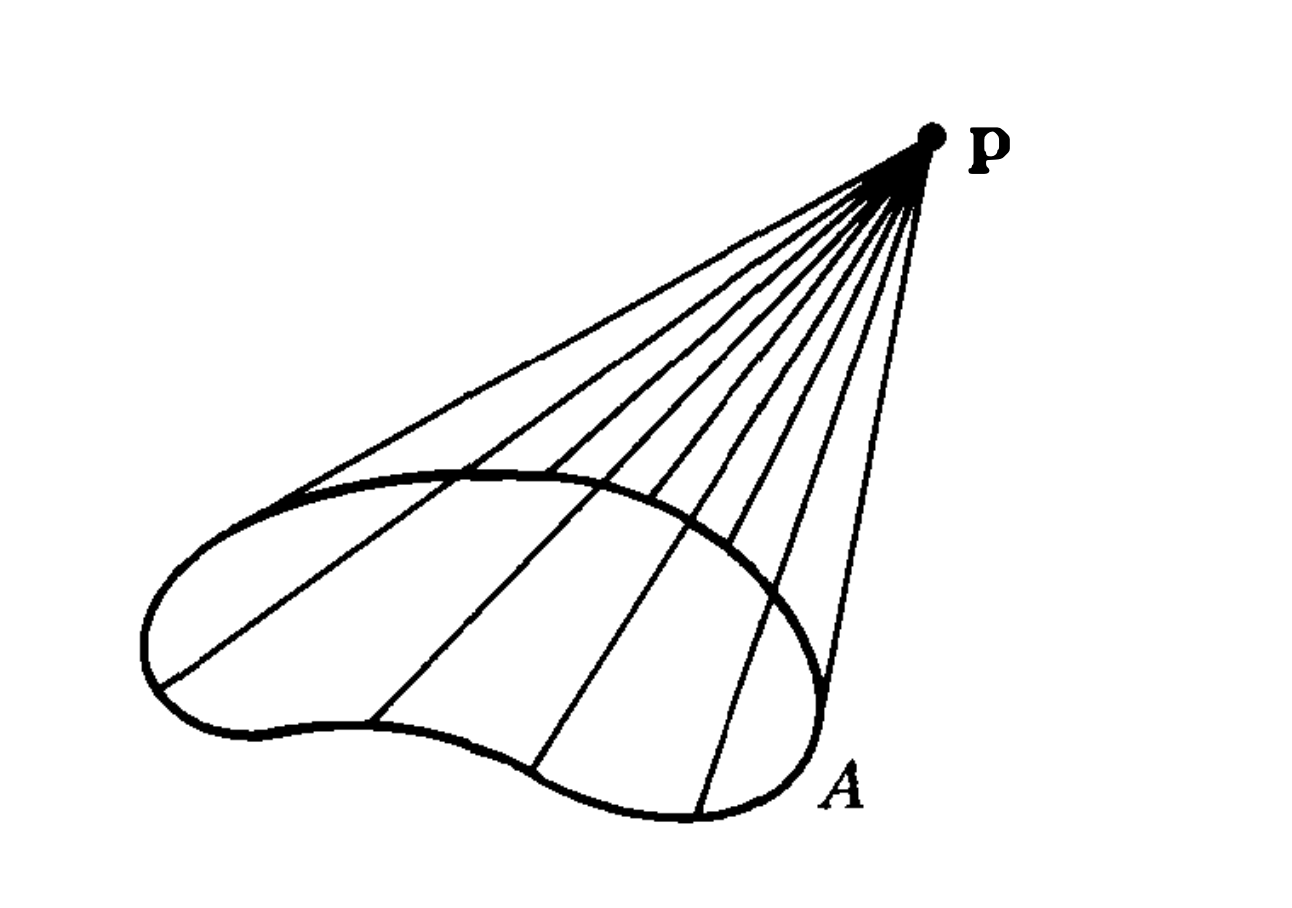
\includegraphics[scale=0.3]{images/Screenshot 2023-01-21 at 16.55.12.png}
        \caption{A cone in $\R^3$}
    \end{figure}
\end{definition}
\noindent\textbf{Remark}:
\begin{itemize}
    \item Just like the coordinate transformations we have learnt, we can use $n$ parameters $(m_1,\cdots,m_n)$ to represent any points $x=(x_1,\cdots,x_n)$ in the open cone $S$.
    Given $x\in S$, we can project $x$ along the line joining $p,x$ to a point $(m_1,\cdots,m_{n-1})$ on the hyperplane $A$, let $m_n$ denote the relative hight on the line. Therefore 
    $$g(m_1,\cdots,m_{n-1},m_n)=(m_n(p_1-m_1)+m_1,\cdots,m_n(p_{n-1}-m_{n-1})+m_{n-1},p_nm_n)$$
    \item $g$ is indeed a diffeomorphism because 
    $$\det(Dg(\vec{m}))=\det(\begin{bmatrix}
        -m_n+1& 0 & \cdots & 0 & p_1-m_1\\
        0 & -m_n+1 & \cdots & 0 & p_2-m_2\\
        \vdots & \vdots & \ddots & \vdots & \vdots\\
        0 & 0 & \cdots & -m_n+1 & p_{n-1}-m_{n-1}\\
        0 & 0 & \cdots & 0 & p_n
    \end{bmatrix})=(-m_n+1)^{n-1}>0$$
    \item If we want to integrate a fuction $f:S\longrightarrow\R$, we can use the change of variable theorem to convert the integral to function $(f\circ g)(-m_n+1)^{n-1}$ on the set $A\times(0,1)$.
\end{itemize}

\begin{theorem}
    Given the volume $v(A)$, we can get $$v(S)=\frac{p_n}{n}v(A)$$
\end{theorem}
\noindent\textbf{Remark}:
\begin{itemize}
    \item This formula corresponds the formula we learnt for 3-dimensional cone in elementary school.
\end{itemize}

\begin{theorem}
    The centroid $c(S)$ of $S$ lies on the line segment joining $c(A)$ and $p$. Explicitly $$c(S)=\frac{n}{n+1}(c(A),0)+\frac{1}{n+1}p$$
\end{theorem}

\begin{definition}
    We will denote the closed ball of radius $a$ in $\R^n$ by $B^n(a)$.
    We will use the general term $\lambda_n$ to denote $v(B^n(1))$.
\end{definition}

\begin{theorem}
    $$v(B^n(a))=v(B^n(1))\cdot a^n=\lambda_na^n$$
\end{theorem}

\begin{theorem}
    $\lambda_n$ has the recurrsion $$\lambda_n=\frac{2\pi}{n}\lambda_{n-2}$$
\end{theorem}

\begin{theorem}
    \begin{equation}
        \lambda_n=
        \begin{cases}
            \frac{(2\pi)^{\frac{n}{2}}}{n!!}\text{\quad for n even}\\
            \frac{2(2\pi)^{\frac{n-1}{2}}}{n!!}\text{\quad for n odd}
        \end{cases}
    \end{equation}
\end{theorem}

\begin{definition}
    We use $B_+^n(a)$ to denote the upper half n-ball.
\end{definition}

\begin{theorem}
    \begin{equation}
        \begin{split}
            c(B_+^n(a)) &= (0,\cdots,0,\frac{2a}{n+1}\times\frac{\lambda_{n-1}}{\lambda_n})\\
            &=\frac{n}{n+1}(0,0,c(B_+^{n-2}(a)))
        \end{split}
    \end{equation}
\end{theorem}

\subsection{The Meaning of Determinant}

\begin{definition}
    Let $A$ be an n by n matrix. Let $h:\R^n\longrightarrow\R^n$ be the linear transformation $h(x)=A\cdot x$. Then
    $$v(h(S))=|\det(A)|\cdot v(S)$$
\end{definition}

\begin{definition}
    Let $\vec{a_1},\cdots,\vec{a_k}$ be independent vectors in $\R^n$. We define the \underline{k-dimensional parallelopiped} to be 
    $$\mathcal{P}(\vec{a_1},\cdots,\vec{a_k})=\{x=c_1\vec{a_1}+\cdots+c_k\vec{a_k}: 0\leq c_i \leq 1\}$$
    The vectors $\vec{a_1},\cdots,\vec{a_k}$ are called the \underline{edges} of $\mathcal{P}$.
    \begin{figure}[H]
        \centering
        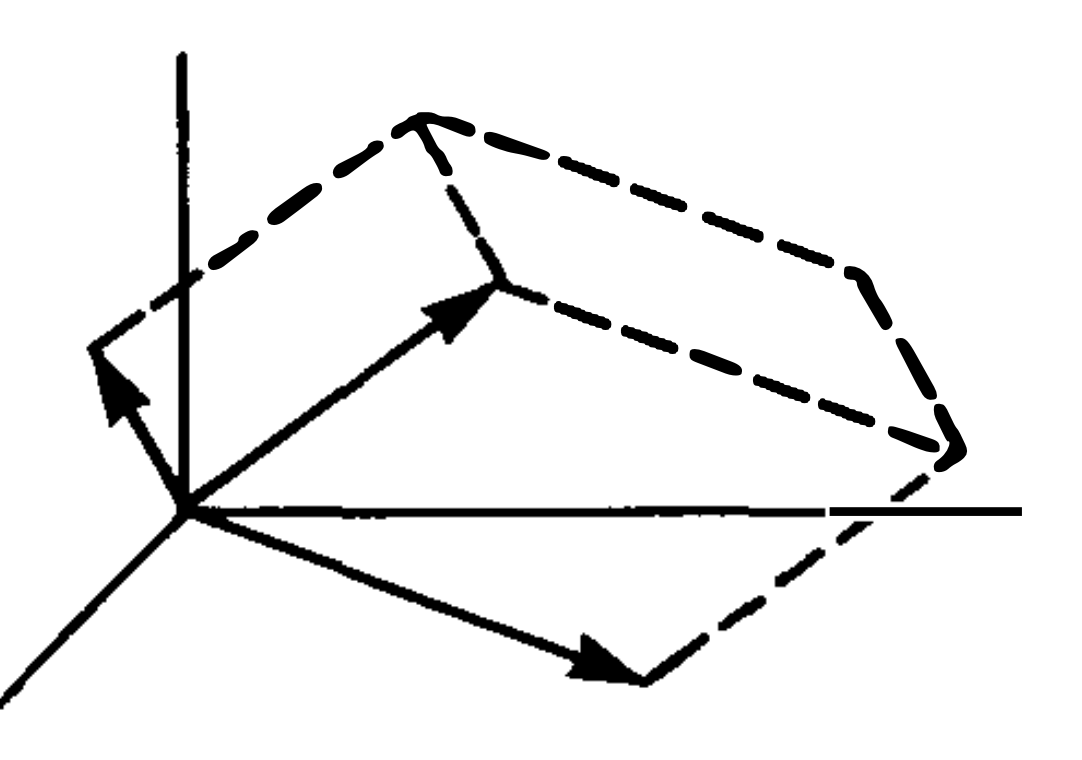
\includegraphics[scale=0.3]{images/Screenshot 2023-01-15 at 23.58.43.png}
        \caption{picture of a parallelopiped in $\R^3$}
    \end{figure}
\end{definition}

\begin{theorem}[The volume of n-dim parallelopiped in $\R^n$]
    Let $\vec{a_1},\cdots,\vec{a_n}$ be independent vectors in $\R^n$.
    Let $A=[\vec{a_1}\cdots\vec{a_n}]$ be the n by n matrix with columns $\vec{a_1},\cdots,\vec{a_n}$. Then
    $$v(\mathcal{P}(\vec{a_1},\cdots,\vec{a_n}))=|\det(A)|$$
\end{theorem}
\begin{corollary}
    Let $\vec{a_1},\vec{a_2},\vec{a_3}$ be edges of a parallelopiped $\mathcal{P}(\vec{a_1},\vec{a_2},\vec{a_3})$ in $\R^3$. Then
    $$\mathcal{P}(\vec{a_1},\vec{a_2},\vec{a_3})=|\det(\begin{bmatrix}
        \vec{a_1}&\vec{a_2}&\vec{a_3}
    \end{bmatrix})|=|\vec{a_1}\cdot(\vec{a_2}\times\vec{a_3})|$$
\end{corollary}
\noindent\textbf{Remark}:
\begin{itemize}
    \item Intuitively, $\vec{a_2}\times\vec{a_3}$ is the area of the base side, $\vec{a_1}$ is the height.
\end{itemize}

\begin{definition}
    Let $V$ be an n-dimensional vector space. An n-tuple $(\vec{a_1},\cdots,\vec{a_n})$ of independent vecors in $V$ is called an \underline{n-frame} in $V$.
\end{definition}

\begin{definition}
    In $\R^n$, we call a frame $(\vec{a_1},\cdots,\vec{a_n})$
    \begin{itemize}
        \item \underline{right-handed} if $\det(\begin{bmatrix}
            \vec{a_1} & \cdots & \vec{a_n}
        \end{bmatrix})>0$
        \item \underline{left-handed} if $\det(\begin{bmatrix}
            \vec{a_1} & \cdots & \vec{a_n}
        \end{bmatrix})<0$
    \end{itemize}
    \begin{figure}[H]
        \centering
        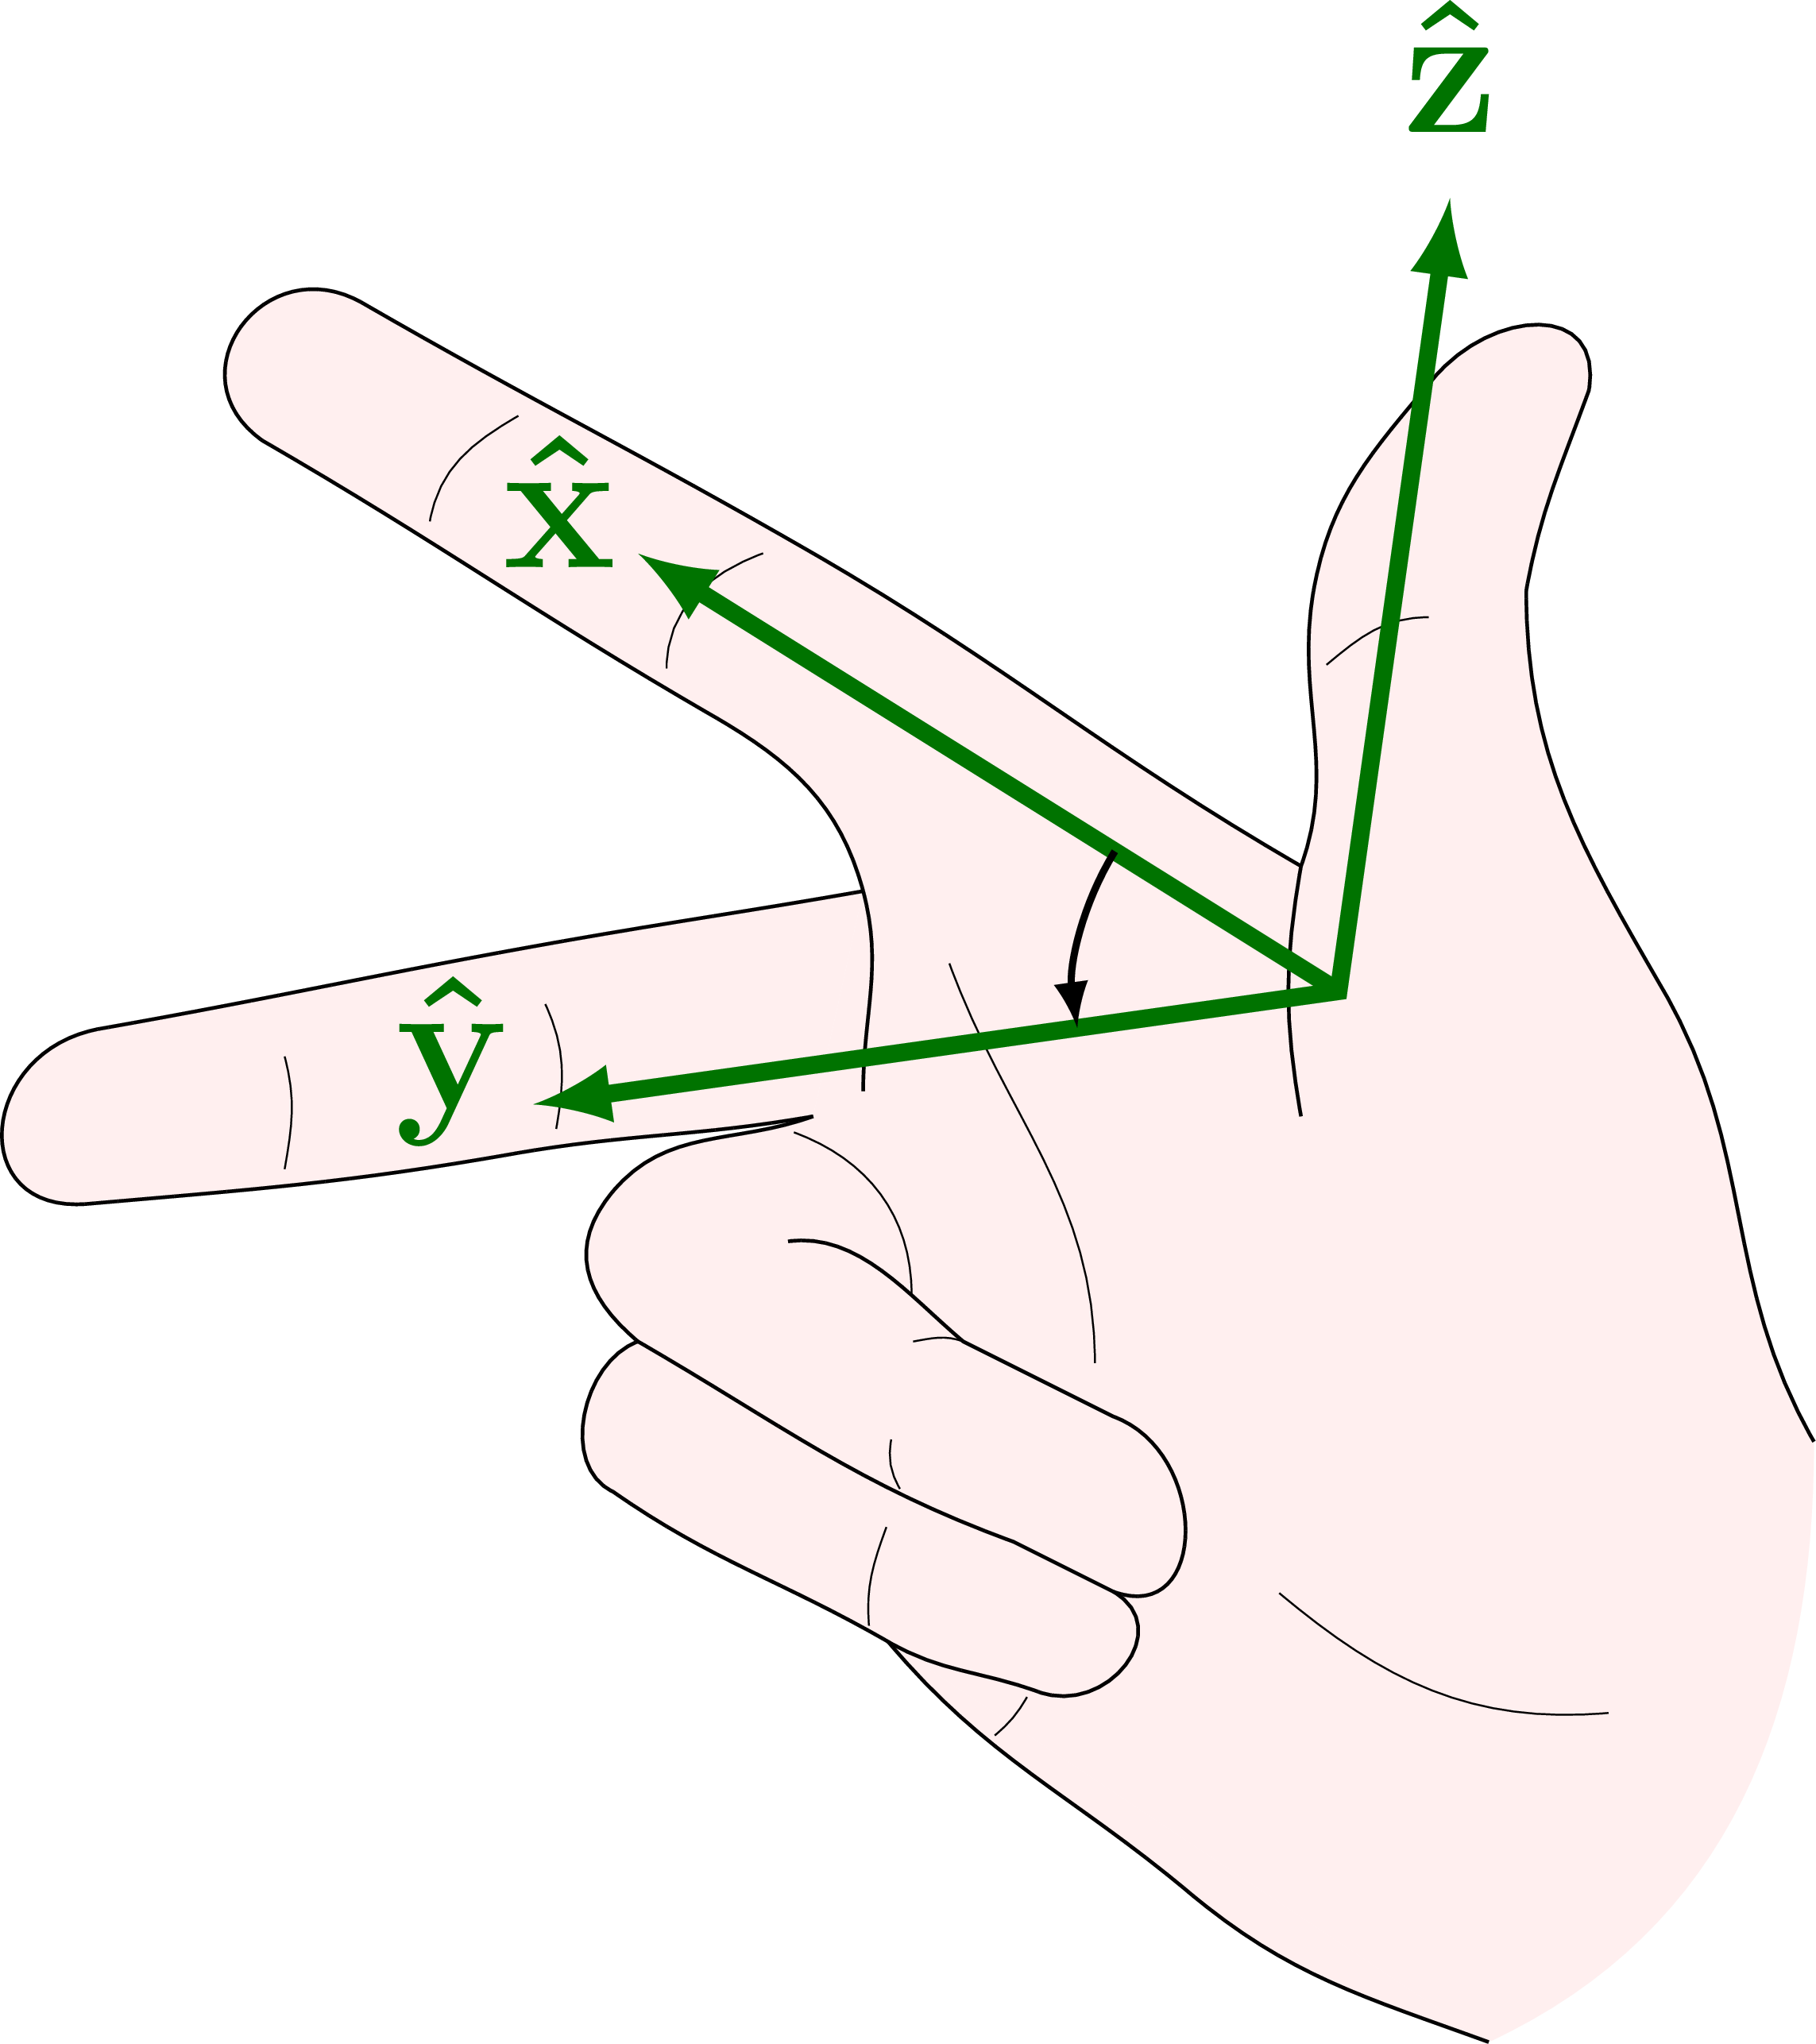
\includegraphics[scale=0.08]{images/righthand_rule-002.png}
        \caption{picture of a right-handed frame}
    \end{figure}
\end{definition}

\begin{definition}
    In $\R^n$ we have two \underline{orientations}:
    \begin{itemize}
        \item the collection of all right-handed frames in $\R^n$
        \item the collection of all left-handed frames in $\R^n$
    \end{itemize}
    Given a isomorphism $T:\R^n\longrightarrow V$ we can define the two \underline{orientations} of $V$:
    \begin{itemize}
        \item the collection of the forms $(T(\vec{a_1},\cdots,\vec{a_n}))$ where $(\vec{a_1},\cdots,\vec{a_n})$ is a right-handed frame in $\R^n$.
        \item the collection of the forms $(T(\vec{a_1},\cdots,\vec{a_n}))$ where $(\vec{a_1},\cdots,\vec{a_n})$ is a left-handed frame in $\R^n$.
    \end{itemize}
\end{definition}

\begin{theorem}
    Let $C$ be a non-singular n by n matrix. Let $h:\R^n\longrightarrow\R^n$ be the linear transformation $h(x)=C\cdot x$. Let $(\vec{a_1},\cdots,\vec{a_n})$ be a frame of $\R^n$.
    \begin{itemize}
        \item If $\det(C)>0$, then the frame $(\vec{a_1},\cdots,\vec{a_n})$ and the frame $(h(\vec{a_1}),\cdots,h(\vec{a_n}))$ belong to the same orientation. In this case, we say $h$ is \underline{orientation-preserving}.
        \item If $\det(C)<0$, then the frame $(\vec{a_1},\cdots,\vec{a_n})$ and the frame $(h(\vec{a_1}),\cdots,h(\vec{a_n}))$ belong to the opposite orientation. In this case, we say $h$ is \underline{orientation-reversing}.
    \end{itemize}
\end{theorem}

\subsection{Isometries Preserve Volume}

\begin{definition}\
    \begin{enumerate}
        \item The set $\{\vec{a_1},\cdots,\vec{a_k}\}$ is \underline{orthogonal} if $\forall i,j\in\{1,\cdots,k\}.i\neq j\implies \innerp{\vec{a_i}}{\vec{a_j}}=0$
        \item The set $\{\vec{a_1},\cdots,\vec{a_k}\}$ is \underline{orthonormal} if it is orthogonal and $\forall i\in\{1,\cdots,k\}.\innerp{\vec{a_i}}{\vec{a_i}}=1$
    \end{enumerate}
\end{definition}

\begin{definition}
    An n by n matrix $A$ is called an \underline{orthogonal matrix} if the columns of $A$ form an orthonormal set. A linear transformation $h(x)=A\cdot x$ is called an \underline{orthogonal transformation} if $A$ is an orthogonal matrix.
\end{definition}

\begin{theorem}
    A matrix $A$ is orthogonal if and only if $A^T=A^{-1}$.
\end{theorem}

\begin{corollary}
    If $A$ is orthogonal, then $\det(A)=1\text{ or }-1$.
\end{corollary}

\begin{theorem*}
    All the orthogonal n by n real matrix forms a group, which is called \underline{orthogonal group}, denoted as $O(n,\R)$.
\end{theorem*}

\begin{definition}
    The function $h:\R^n\longrightarrow\R^n$ is called a \underline{(euclidean) isometry} if for all $x,y\in\R^n$
    $$\norm{h(x)-h(y)}=\norm{x-y}$$
\end{definition}

\begin{theorem}
    Let $h:\R^n\longrightarrow\R^n$ that fix the origin.($h(0)=0$)
    \begin{enumerate}
        \item $h$ is an isometry if and only if $h$ preserves dot product.
        \item $h$ is an isometry if and only if $h$ is an orthogonal transformation.
    \end{enumerate}
\end{theorem}

\begin{theorem}
    $h$ is an isometry if and only if it equals an orthogonal transformation followed by a translation, that is, if and only if $h$ has the form $$h(x)=A\cdot x+p$$
    where $A$ is an orthogonal matrix.
\end{theorem}

\begin{theorem}
    If $h$ is an isometry and $S$ is a rectifiable set, then $h(S)$ is rectifiable and $v(h(S))=v(S)$.
\end{theorem}
\chapter{Manifolds in $\R^n$}

\section{k-dimensional Parallelopiped in $\R^n$}

\begin{lemma}
    Let $W$ be a linear subspace of $\R^n$ of dimension $k$. Then there is an orthonormal basis for $\R^n$ whose first $k$ elements form a basis for $W$.
\end{lemma}

\begin{theorem}
    Let $W$ be a k-dimensional linear subspace of $\R^n$. There is an orthogonal transformation $h:\R^n\longrightarrow\R^n$ that carries $W$ onto the subspace $\R^k\times0$ of $\R^n$.
\end{theorem}

\begin{definition}
    Given vectors $\vec{x_1},\cdots,\vec{x_k}$ is $\R^n$. 
    Define the n by k matrix $$X=\begin{bmatrix}
        \vec{x_1} & \cdots & \vec{x_k}
    \end{bmatrix}$$
    we define the \underline{k-dimensional volume} of the parallelopiped $\mathcal{P}(\vec{x_1},\cdots,\vec{x_k})$ to be 
    $$V(\vec{x_1},\cdots,\vec{x_k})=\sqrt{\det(X^T\cdot X)}$$
\end{definition}
\noindent\textbf{Example}:
\begin{itemize}
    \item Consider two independent vectors $\vec{a},\vec{b}$ in $\R^3$. Define the 3 by 2 matrix $$X=\begin{bmatrix}
        \vec{a} & \vec{b}
    \end{bmatrix}$$
    Let $\theta$ denote the angle between $\vec{a},\vec{b}$, then 
    \begin{equation*}
        \begin{split}
            V^2(\vec{a},\vec{b}) &= V^2(X)\\
            &= \det(\begin{bmatrix}
                \norm{\vec{a}}^2 & \innerp{\vec{a}}{\vec{b}}\\
                \innerp{\vec{b}}{\vec{a}} & \norm{\vec{b}}^2
            \end{bmatrix})\\
            &= \norm{\vec{a}}^2 \norm{\vec{b}}^2(1-\cos^2\theta)\\
            &= \norm{\vec{a}}^2 \norm{\vec{b}}^2\sin^2\theta
        \end{split}
    \end{equation*}
    \begin{figure}[H]
        \centering
        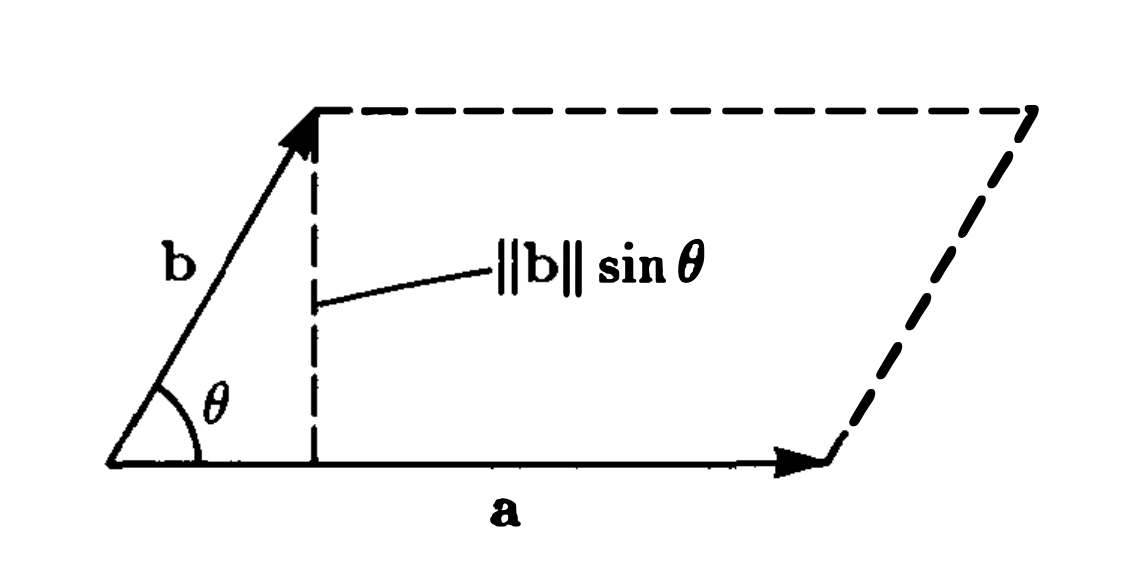
\includegraphics[scale=0.3]{images/Screenshot 2023-01-16 at 02.13.22.png}
        \caption{picture of 2-dimensional volume in $\R^3$}
    \end{figure}
\end{itemize}

\begin{theorem}[Properties of k-dim volume in $\R^n$]\
    \begin{enumerate}
        \item If $h:\R^n\longrightarrow\R^n$ is an orthogonal transformation, then $$V(h(\vec{x_1}),\cdots,h(\vec{x_k}))=V(\vec{x_1},\cdots,\vec{x_k})$$
        \item If $\vec{y_1},\cdots,\vec{y_k}$ belong to the subspace $\R^k\times 0$ of $\R^n$, such that $$\vec{y_i}=\begin{bmatrix}
            \vec{z_i}\\
            \vec{0}
        \end{bmatrix}$$
        where $\vec{z_i}\in\R^k$, $\vec{0}\in\R^{n-k}$, then 
        $$V(\vec{y_1},\cdots,\vec{y_k})=|\det(\begin{bmatrix}
            \vec{z_1} & \cdots & \vec{z_k}
        \end{bmatrix})|$$
        \item $\vec{x_1},\cdots,\vec{x_k}$ are linear dependent if and only if $V(\vec{x_1},\cdots,\vec{x_k})\neq0$
    \end{enumerate}
\end{theorem}

\begin{definition}
    Let $\vec{x_1},\cdots,\vec{x_k}$ be vectors in $\R^n$ with $k\leq n$. Define the n by k matrix $$X=\begin{bmatrix}
        \vec{x_1} & \cdots \vec{x_k}
    \end{bmatrix}$$
    Define an ascending k-tuple from $\{1,\cdots,n\}$ $$I=(i_1,\cdots,i_k)$$
    where $1\leq i_1\leq i_2\leq \cdots \leq i_k\leq n$
    Finally, we define the k by k matrix $X_I$ or $X(i_1,\cdots,i_k)$ to be the submatrix of $X$ consisting of rows $i_1,\cdots,i_k$.
\end{definition}

\begin{theorem*}
    Let $X$ be an n by k matrix with $k\leq n$. Then
    $$V^2(X)=\sum_{[I]}[\det(X_I)]^2$$
    where the symble $[I]$ indicates that the summaton extends over all ascending k-tupes from $\{1,\cdots,n\}$.
\end{theorem*}
\noindent\textbf{Remark}:
\begin{itemize}
    \item This theorem may be thought of as a Pythagorean theorem for k-volume. It states that the square of the volume of a k-parallelopiped $\mathcal{P}$ in $\R^n$ is equal to the sum of the squares of the volumes of the k-parallelopipeds obtained by projecting $\mathcal{P}$ onto the various coordinate k-planes of $\R^n$.
    \item Consider the following picture of a 2-parallelopiped(parallelogram) in $\R^3$.
    \begin{figure}[H]
        \centering
        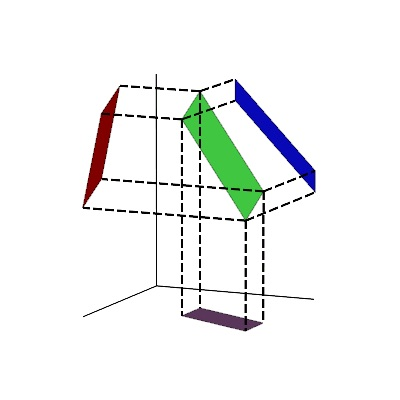
\includegraphics[scale=0.6]{images/vectors_66.jpeg}
        \caption{a 2-parallelopiped(parallelogram) in $\R^3$}
    \end{figure}
    Let $V$ denotes the volume of the 2-parallelopiped, which is the green part. Let $V_r,V_b,V_p$ denotes the volume of the red, blue, purple part respectively.
    This theorem tells us $$V^2=V_r^2+V_b^2+V_p^2$$
\end{itemize}

\section{Parametrized Manifold in $\R^n$}

\begin{definition}
    Let $k\leq n$. Let $A$ be open in $\R^k$, and let $\alpha:A\longrightarrow \R^n$ be a map of class $C^r$.
    The set $Y=\alpha(A)$, together with the map $\alpha$, constitute what is called \underline{parametrized-manifold} of dimension $k$. 
    We denote this parametrized-manifold by $Y_{\alpha}$ and we define the \underline{(k-dimensional) volume} of $Y_{\alpha}$ by the equation
    $$v(Y_{\alpha})=\int_AV(D\alpha)$$
\end{definition}
\noindent\textbf{Remark}:
\begin{itemize}
    \item Consider $A$ is the interior of a closed rectangle $Q$ in $\R^k$. Let $P$ be a partition of the rectangle $Q$.
    Consider one of the very small subrectangles $$R=[a_1,a_1+h_1]\times\cdots\times[a_k,a_k+h_k]$$
    This subtangle is maped to a curved rectangle $\alpha(R)$ in $\R^n$. Since the subrectangle is very very small, and the continuous function $\alpha$ has the locally linearity property, so the curved rectangle $\alpha(R)$ can be considered as a very small parallelopiped.
    \begin{figure}[ht]
        \centering
        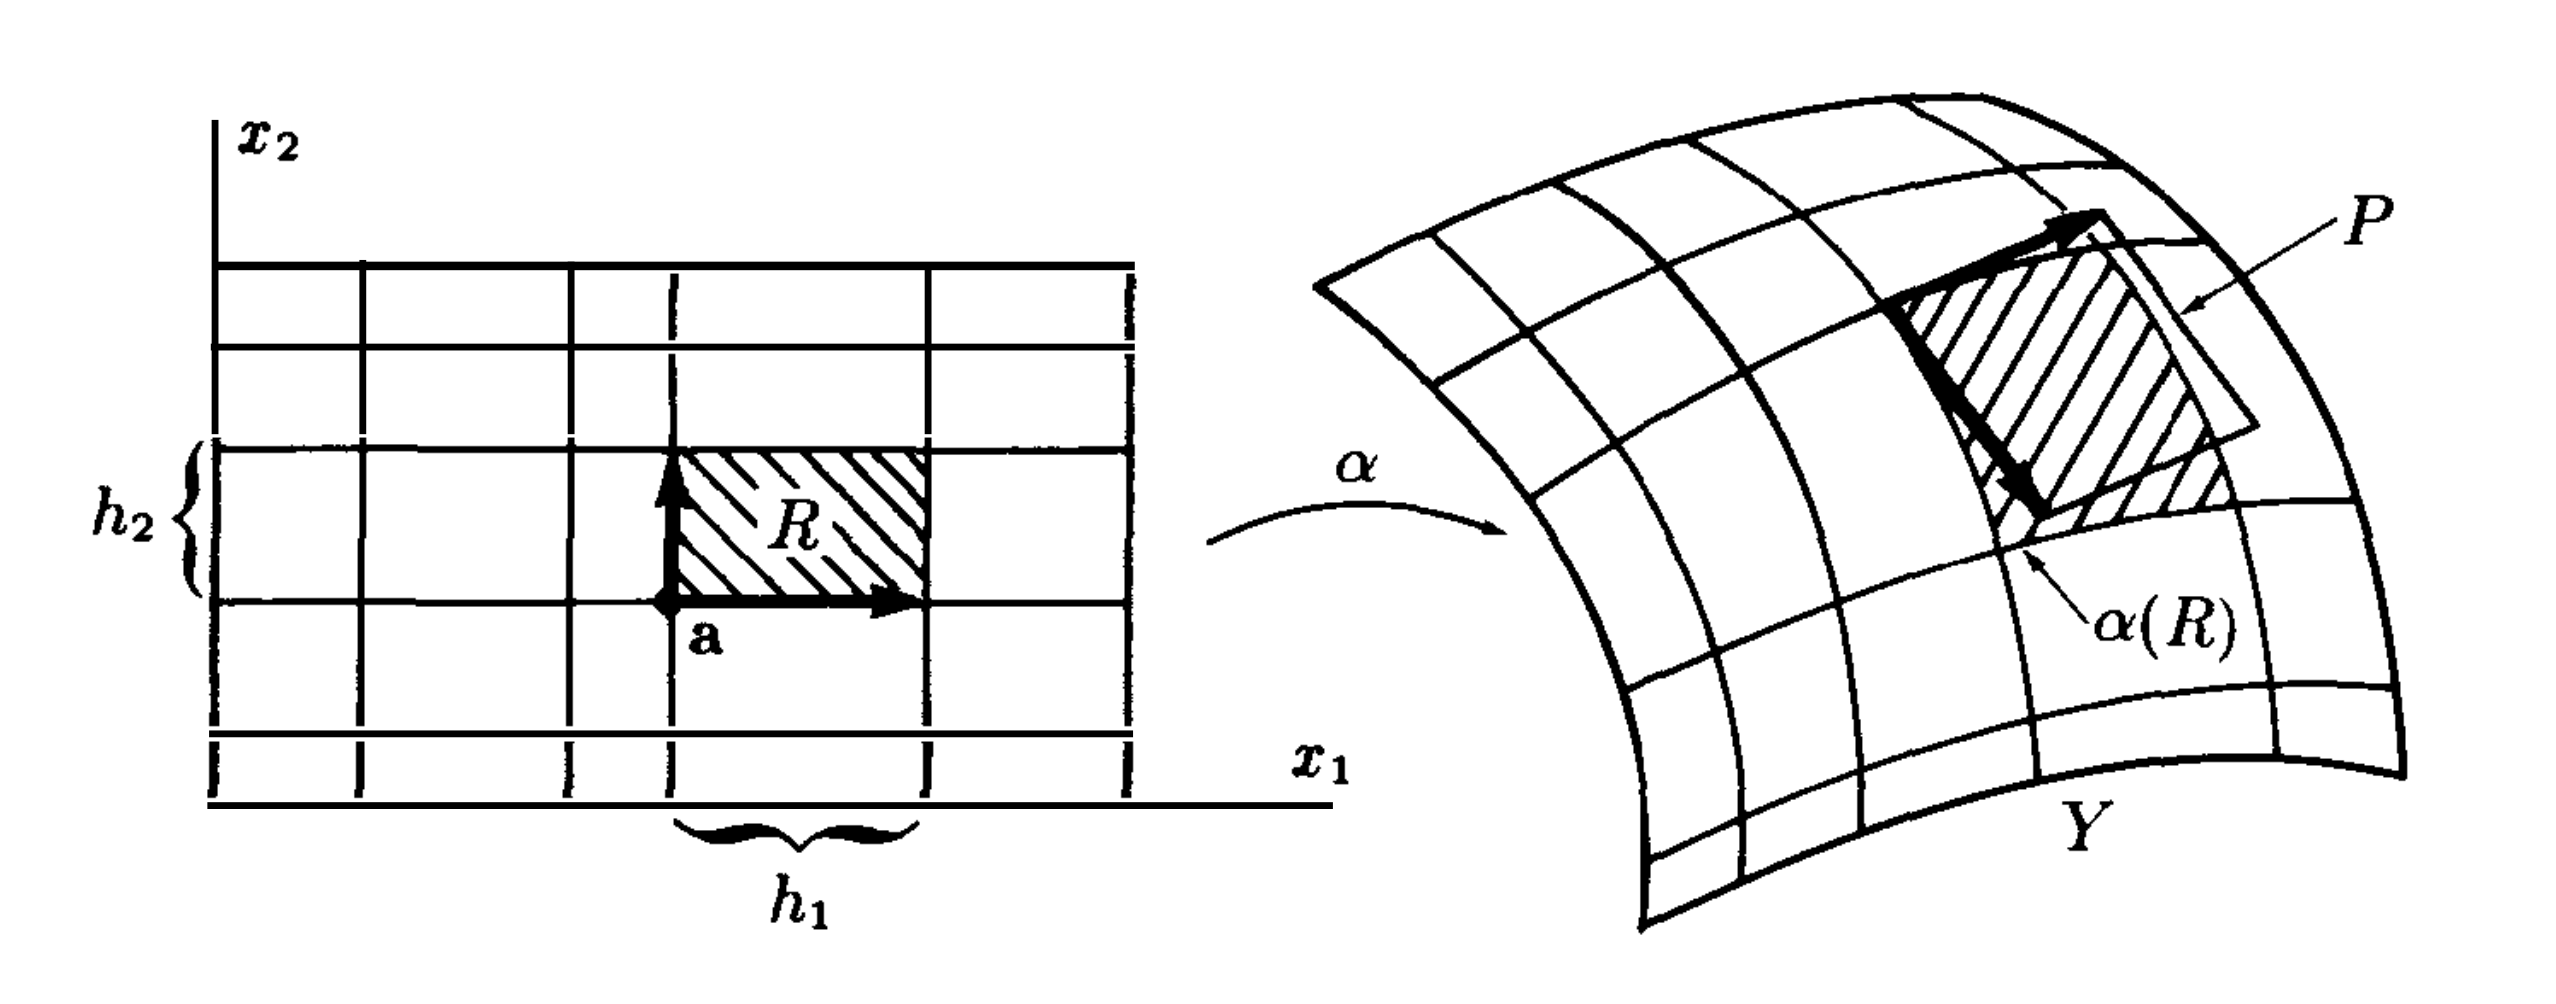
\includegraphics[scale=0.3]{images/Screenshot 2023-01-18 at 13.34.54.png}
        \caption{$\alpha:Int(Q)\subset\R^2\to\R^n$}
    \end{figure}
    \item For the point $\vec{a}=(a_1,\cdots,a_k)$, the jacobian matrix(total derivative) $D\alpha(\vec{a})$ is the linear approximation of the transformation $\alpha$ at the point $\vec{a}$.
    So the volume of the parallelopiped $\alpha(R)$ is $$V(D\alpha(\vec{a})h_1\vec{e_1},\cdots,D\alpha(\vec{a})h_k\vec{e_k})=(h_1\times\cdots\times h_k)V(D\alpha(\vec{a}))=V(D\alpha(\vec{a}))\cdot v(R)$$
    Then we sum over all subrectangles $R$ determined by $P$ to get the approximation of the volume of $Y_{\alpha}(A)$ $$\sum_{R}V(D\alpha)v(R)$$
    \item As the partition gets more and more finer, the summation becomes the integral over $A$, so we get
    $$v(Y_{\alpha})=\int_AV(D\alpha)$$
\end{itemize}

\begin{definition}
    Let $k\leq n$. Let $A$ be open in $\R^k$, and let $\alpha:A\longrightarrow \R^n$ be a map of class $C^r$. Let $Y=\alpha(A)$.
    Let $f:Y\longrightarrow\R$ be a real-valued continuous function. We define the \underline{integral} of $f$ over $Y_{\alpha}$ \underline{with respect to volume}, by the equation
    $$\int_{Y_{\alpha}}f\di V=\int_A(f\circ \alpha)V(D\alpha)$$
\end{definition}
\noindent\textbf{Remark}:
\begin{itemize}
    \item $\di V$ can be considered the unit volume of the parametrized-manifold $Y_{\alpha}(A)$. For example. consider $$\alpha:A\subset \R^2\longrightarrow\R^3$$
    The parametrized-manifold $Y_{\alpha}(A)$ is a surfaces in $\R^3$. $\di V$ can be considered the unit area of $Y_{\alpha}(A)$, which is obtained by streching the unit area of $A$ ($\di x \di y$) by $V(D\alpha)$.
    The function $f:Y(A)\longrightarrow\R$ can be thought of the height, so $f\di V$ is the unit volume. Taking the integral over $Y_{\alpha}(A)$ we get the volume we want. This new notation
     corresponds our intuition.
     \item Consider the one dimensional example. Let $\alpha:A\subset\R\longrightarrow B\subset\R$ be a change of variable. The change of variable theorem tells us
     $$\int_Bf(u)\di u=\int_Af(\alpha(x))\alpha'(x)\di x$$
     Similarly, $\di u$ is the new unit length, which is obtained by streching the unit length of $A$ by $\alpha'$.
\end{itemize}

\begin{theorem}[Invariant under reparametrization]
    Let $g:A\longrightarrow B$ be a diffeomorphism of open sets in $\R^k$. Let $\beta:B\longrightarrow\R^n$ be a map of class $C^r$. Let $Y=\beta(B)$.
    Let $\alpha=\beta\circ g$, then $\alpha:A\longrightarrow\R^n$ and $Y=\alpha(A)$. If $f:Y\longrightarrow\R$ is a continnuous function, then $f$ is integrable over $Y_{\alpha}$ if and only if $f$ is integrable over $Y_{\beta}$.
    In this case $$\int_{Y_{\alpha}}f\di V=\int_{Y_{\beta}}f\di V$$
    \begin{figure}[ht]
        \centering
        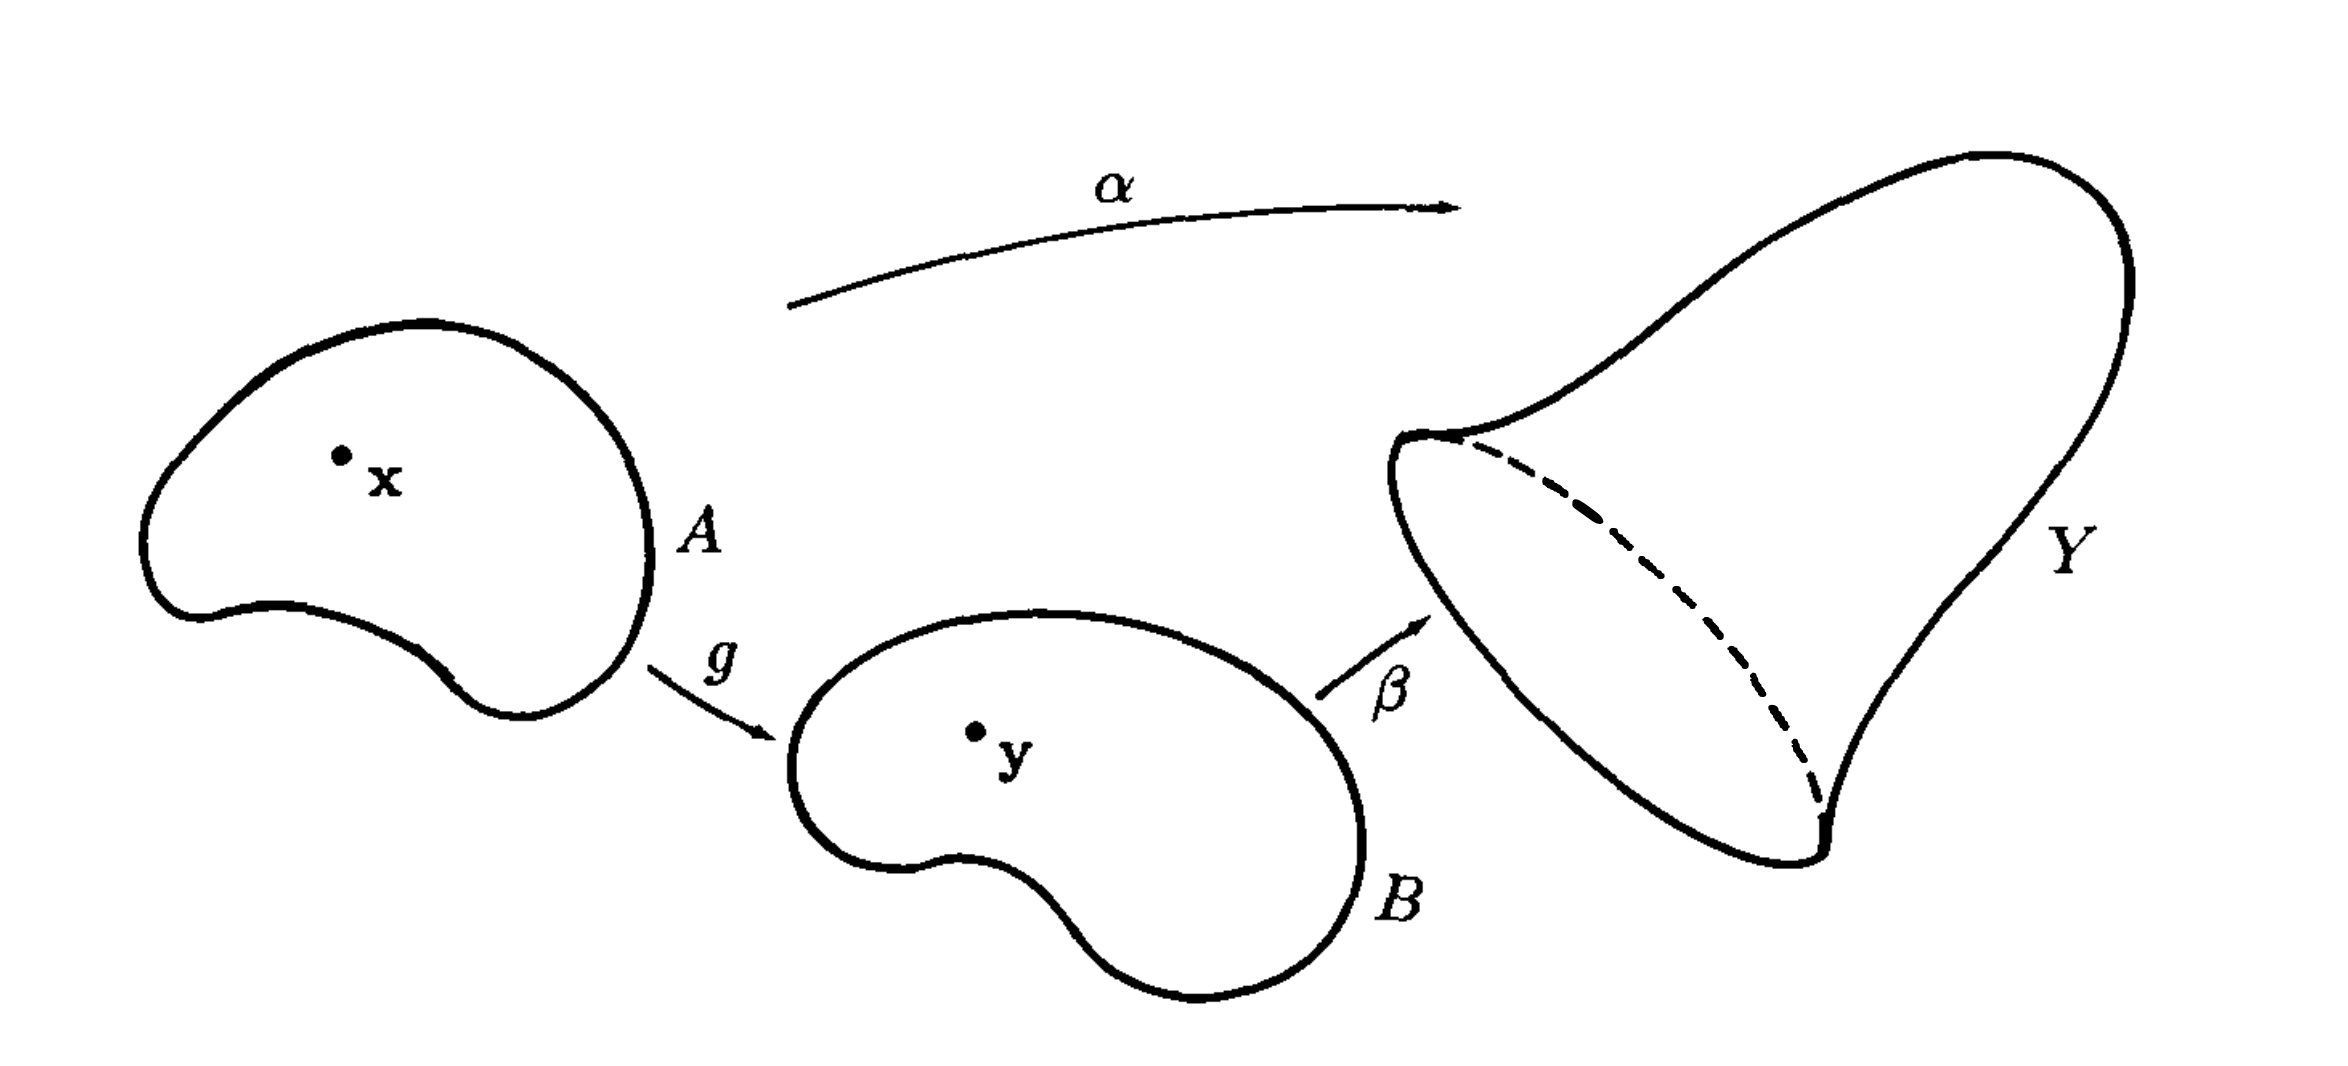
\includegraphics[scale=0.3]{images/Screenshot 2023-01-18 at 14.35.53.png}
        \caption{Invariant under reparametrization}
    \end{figure}
\end{theorem}

\begin{definition}
    Let $A$ be an open set in $\R$. Let $\alpha:A\longrightarrow\R^n$ be a map of class $C^r$. Let $Y=\alpha(A)$. Then $Y_{\alpha}$ is called a \underline{parametrized-curve} in $\R^n$.
    The 1-dimensional volume of $Y_{\alpha}$ is often called its \underline{length}.
\end{definition}

\begin{theorem}
    The length of a parametrized-curve in $\R^n$ is given by the formula
    \begin{equation*}
        v(Y_{\alpha})=\int_AV(D\alpha)=\int_A[(\frac{\di\alpha_1}{\di t})^2+\cdots+(\frac{\di\alpha_n}{\di t})^2]^{\frac{1}{2}}
    \end{equation*}
\end{theorem}
\noindent\textbf{Remark}:
\begin{itemize}
    \item Recall the length of the function $f$ in MAT157 $$l(f)=\int_a^b(1+(f'(t))^2)^{\frac{1}{2}}\di t$$
    In this situation $$\alpha(t)=(t,f(t))$$
    \item Consider a parametrized-curve in $\R^2$ defined by $$\alpha(t)=(a\sin(t),a\cos(t))$$
    Let $A$ be the interval $(0,3\pi)$, can we apply the formula?
    If we apply the formula, then $$\int_{0}^{3\pi}[a^2\sin^2(t)+a^2\cos^2(t)]^{\frac{1}{2}}=3\pi a$$
    We can see this from the picture, since $\alpha$ is not one-to-one, this integral is not the length of the image $B=\alpha(A)$, it can be thought as the distance traveled in time from $0$ to $3\pi$.
    \begin{figure}[ht]
        \centering
        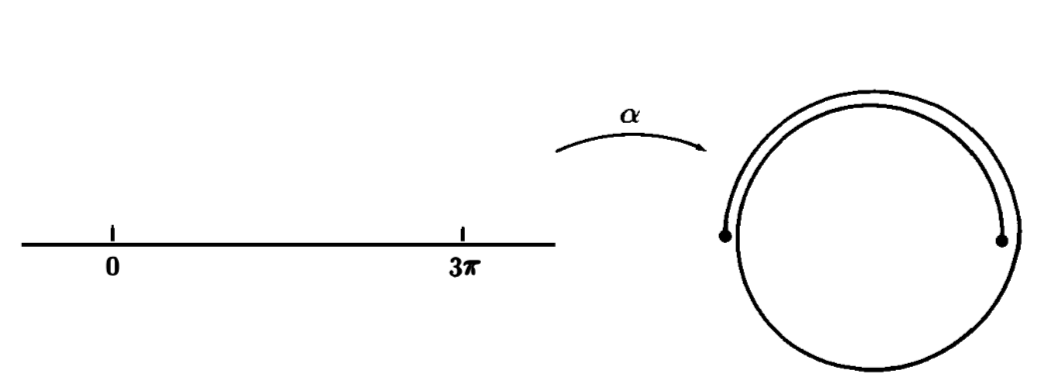
\includegraphics[scale=0.5]{images/Screenshot 2023-01-18 at 16.23.16.png}
        \caption{$\alpha(t)=(a\sin(t),a\cos(t))$ for $0<t<3\pi$}
    \end{figure}
    Although it is useful in physics, we will restrict $\alpha$ to be one-to-one to avoid problems.
\end{itemize}

\begin{definition}
    Let $A$ be open in $\R^2$. Let $\alpha:A\longrightarrow \R^n$ be of class $C^r$. Let $Y=\alpha(A)$.
    Then $Y$ is called a \underline{parametrized-surface} in $\R^n$, and it's 2-dimensional volume is called the \underline{area}
\end{definition}

\begin{theorem}[Area of surface in $\R^3$]
    Let $\alpha:A\subset\R^2\longrightarrow\R^3$ defined as $\alpha(x,y)=(x,y,f(x,y))$, 
    The area of a parametrized-curve in $\R^3$ is given by the formula
    $$v(Y_{\alpha})=\int_A\norm{\frac{\partial \alpha}{\partial x}\times\frac{\partial \alpha}{\partial y}}=\int_A[1+(\frac{\partial f}{\partial x})^2+(\frac{\partial f}{\partial y})^2]^{\frac{1}{2}}$$
    where the symble $\times$ is the cross product.
\end{theorem}
\noindent\textbf{Example}:
\begin{itemize}
    \item Compute the area of a hemisphere in $\R^3$.\\
    Let $\alpha(x,y)=(x,y,f(x,y))$ where $f(x,y)=\sqrt{a^2-x^2-y^2}$ note that $a$ is the radius of the hemisphere. 
    \begin{figure}[ht]
        \centering
        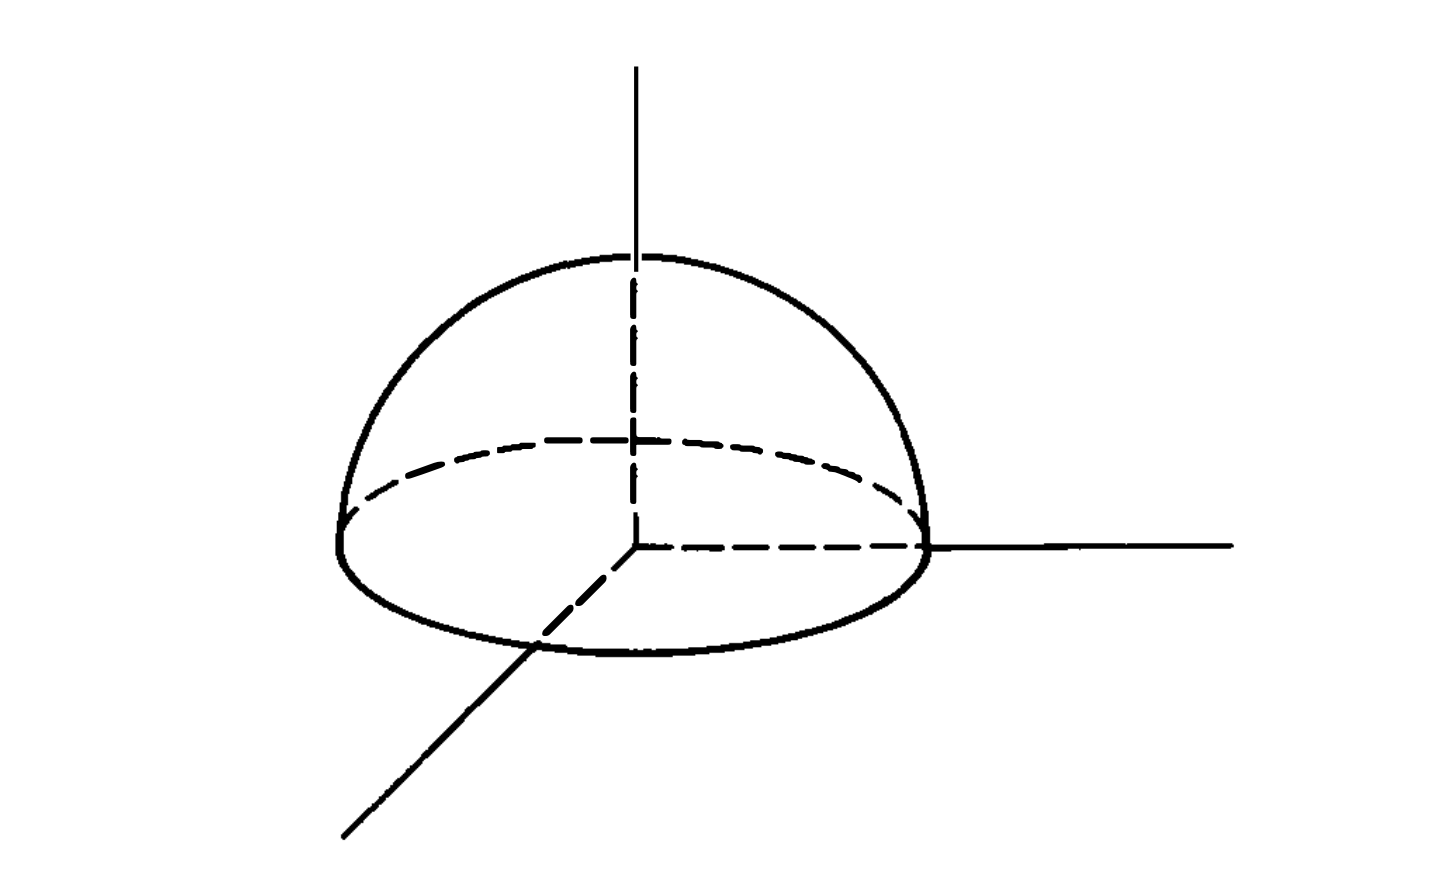
\includegraphics[scale=0.3]{images/Screenshot 2023-01-18 at 20.28.41.png}
        \caption{Picture of a hemisphere}
    \end{figure}
    First, we compute the partial derivatives $$D_1f(x,y)=\frac{-x}{\sqrt{a^2-x^2-y^2}}$$ $$D_2f(x,y)=\frac{-y}{\sqrt{a^2-x^2-y^2}}$$
    By the theorem above $$V(D\alpha(x,y))=[1+(D_1f)^2+(D_2f)^2]^{\frac{1}{2}}=\frac{a}{\sqrt{a^2-x^2-y^2}}$$
    By the definition of integral over $Y_{\alpha}$ with respect to volume, we have 
    $$v(Y_{\alpha})=\int_{Y_{\alpha}}1\di V=\int_{(x,y)\in A}V(D\alpha(x,y))$$
    Let $g:B=(0,a)\times(0,2\pi)\longrightarrow A$ be the polar coordinate transformation. so
    \begin{equation*}
        \begin{split}
            v(Y_{\alpha}) &= \int_{(x,y)\in A}V(D\alpha(x,y))\\
            &= \int_B(V(D\alpha) \circ g)\cdot|\det(Dg)|\\
            &= \int_B\frac{ar}{\sqrt{a^2-(r\cos\theta)^2-(r\sin\theta)^2}}\\
            &= \int_B\frac{ar}{\sqrt{a^2-r^2}}
        \end{split}
    \end{equation*}
    Let $h(r,\theta)=\frac{ar}{\sqrt{a^2-r^2}}$, $h$ is unbouded on $B$, so we must use improper integral. 
    \begin{figure}[ht]
        \centering
        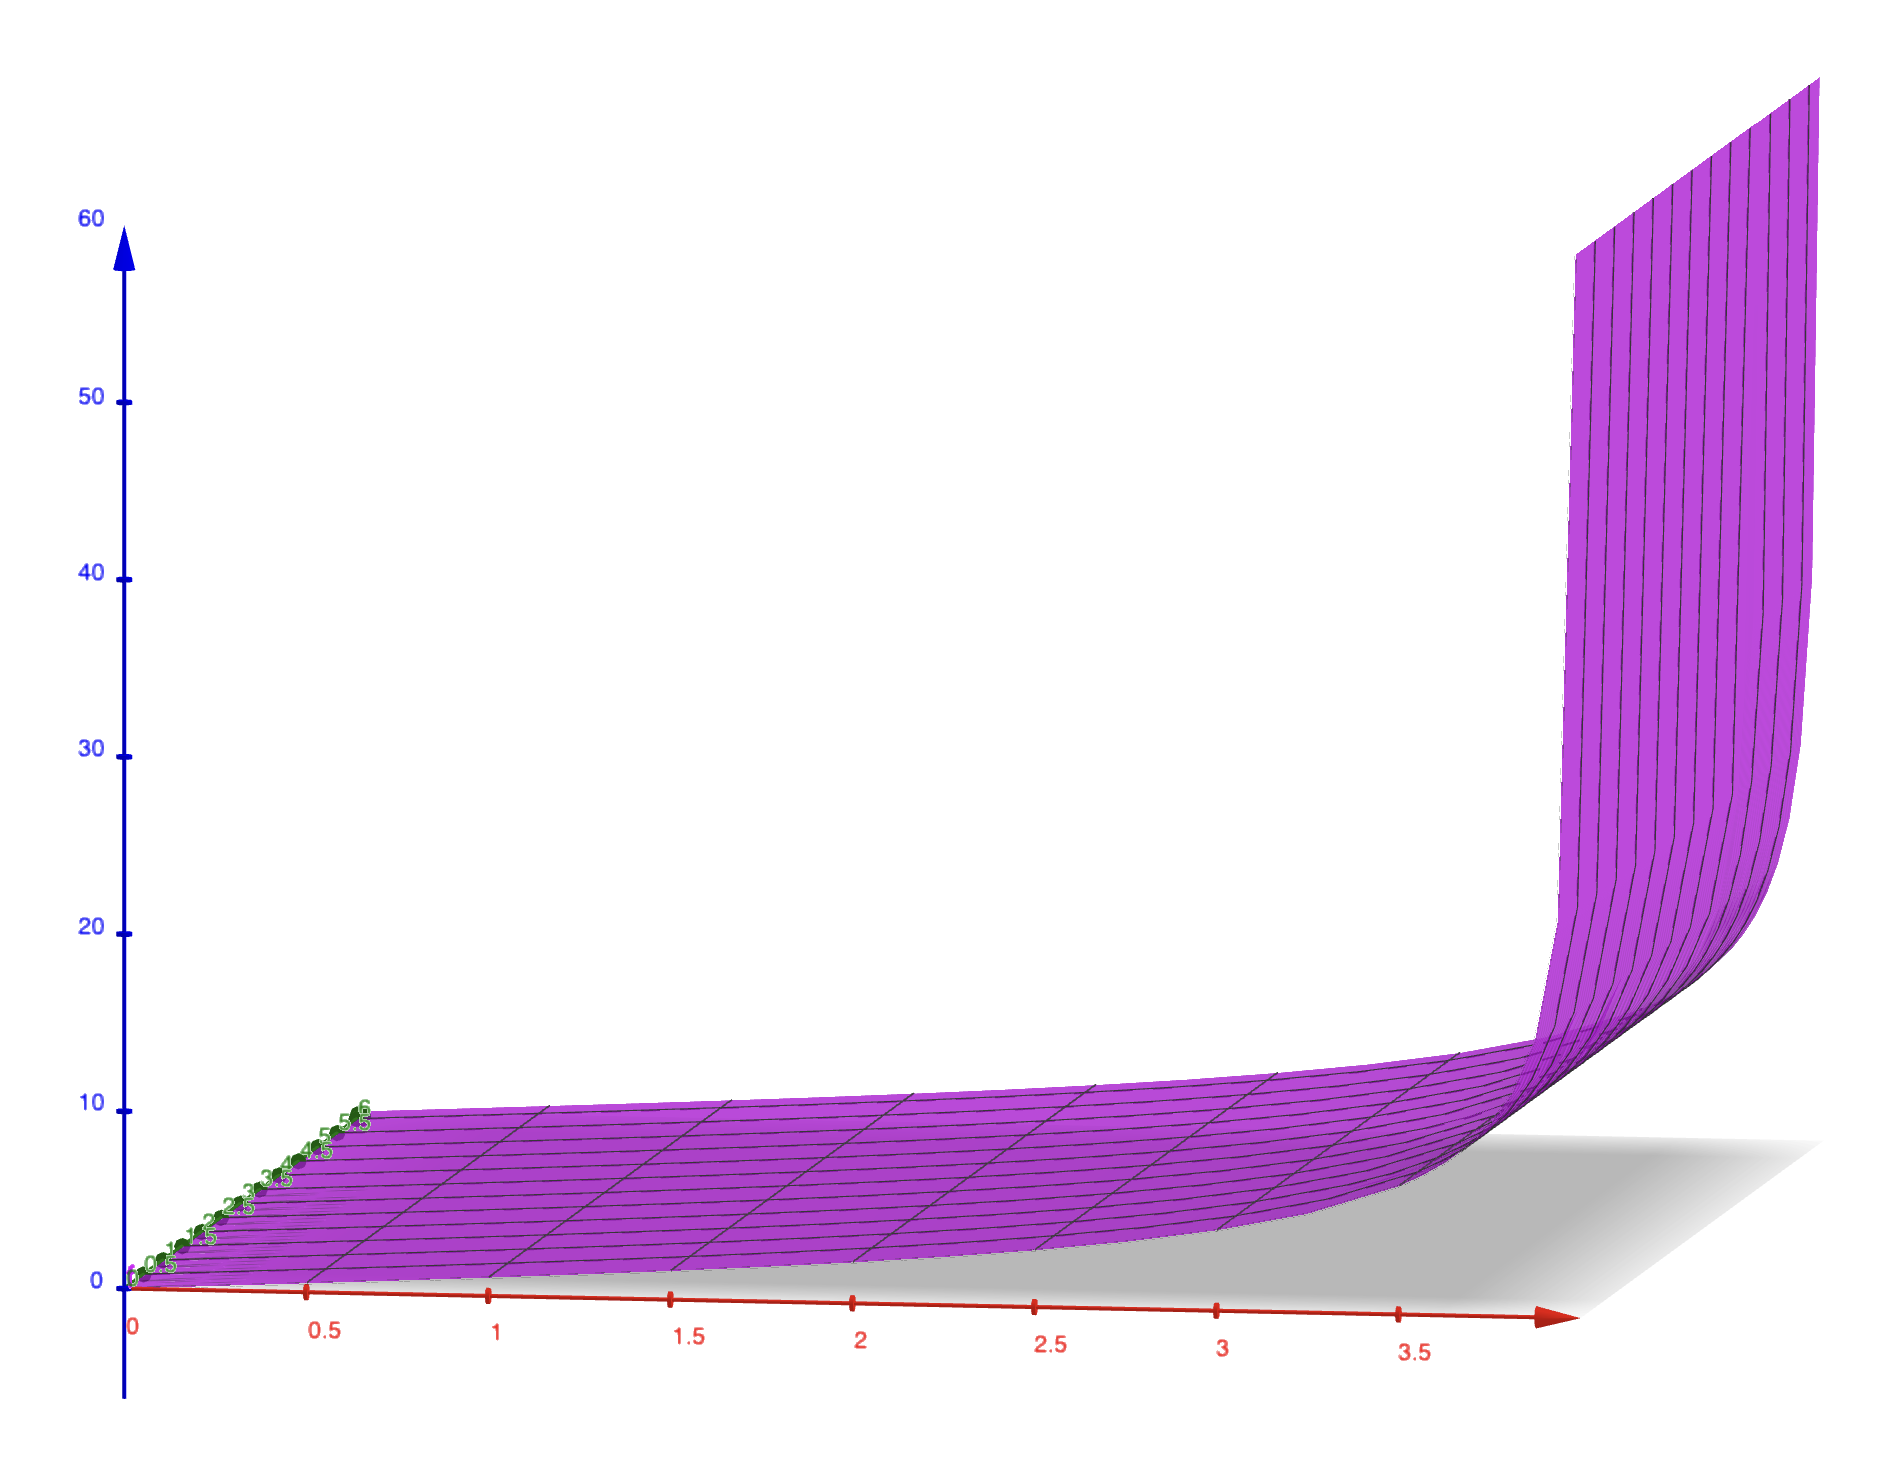
\includegraphics[scale=0.3]{images/Screenshot 2023-01-18 at 19.52.34.png}
        \caption{Picture of $h(r,\theta)$ on the set $B$}
    \end{figure}
    Define 
    $$U_N=(0,a_N)\times(0,2\pi)$$ with $0<a_1<a_2<\cdots<a$ and $\lim_{N\to\infty}a_N=a$.
    Now we can use Fubini theorem on $U_N$.
    \begin{equation*}
        \begin{split}
            \int_{U_N}\frac{ar}{\sqrt{a^2-r^2}} &= \int_{r=0}^{r=a_N}\int_{\theta=0}^{\theta=2\pi}\frac{ar}{\sqrt{a^2-r^2}}\di\theta \di r\\
            &= 2\pi \int_{r=0}^{r=a_N}\frac{ar}{\sqrt{a^2-r^2}}\di r\\
            &= 2\pi(-a\sqrt{a^2-a_N^2}+a\sqrt{a^2})\\
            &= 2\pi(-a\sqrt{a^2-a_N^2}+a^2)
        \end{split}
    \end{equation*}
    Therefore 
    \begin{equation*}
        \begin{split}
            v(Y_{\alpha})&= \lim_{N\to\infty}\int_{U_N}\frac{ar}{\sqrt{a^2-r^2}}\\
            &= \lim_{N\to\infty}2\pi(-a\sqrt{a^2-a_N^2}+a^2)\\
            &= 2\pi a^2
        \end{split}
    \end{equation*}
\end{itemize}

\section{General Manifolds in $\R^n$}

\begin{definition}
    Let $k > 0$. A \underline{k-manifold without boundary} in $\R^n$ of class $C^r$ is a subspace $M\subset \R^n$ having the following property:
    For each $p \in M$, there is an open set $V \subset M$ containing $p$, an open set $U\subset \R^k$ and a continuous bijective map $\alpha: U \longrightarrow V$ such that:
    \begin{itemize}
        \item $\alpha$ is of class $C^r$.
        \item $\alpha^{-1}:V \longrightarrow U$ is continuous.
        \item $D\alpha(x)$ has rank $k$ for each $x \in U$.
    \end{itemize}
    The map $\alpha$ is called a \underline{coordinate patch} on $M$ about $p$.
\end{definition}
\noindent\textbf{Remark}:
\begin{itemize}
    \item In mathematics, a manifold is a topological space that locally resembles Euclidean space near each point.
    \item $rank(D\alpha(x))=k$ means that vectors $D_1\alpha(x),\cdots,D_k\alpha(x)$ are independent at $x$. Geometrically, those vectors span a k-dimensional tangent plane to $M$.
    \begin{figure}[H]
        \centering
        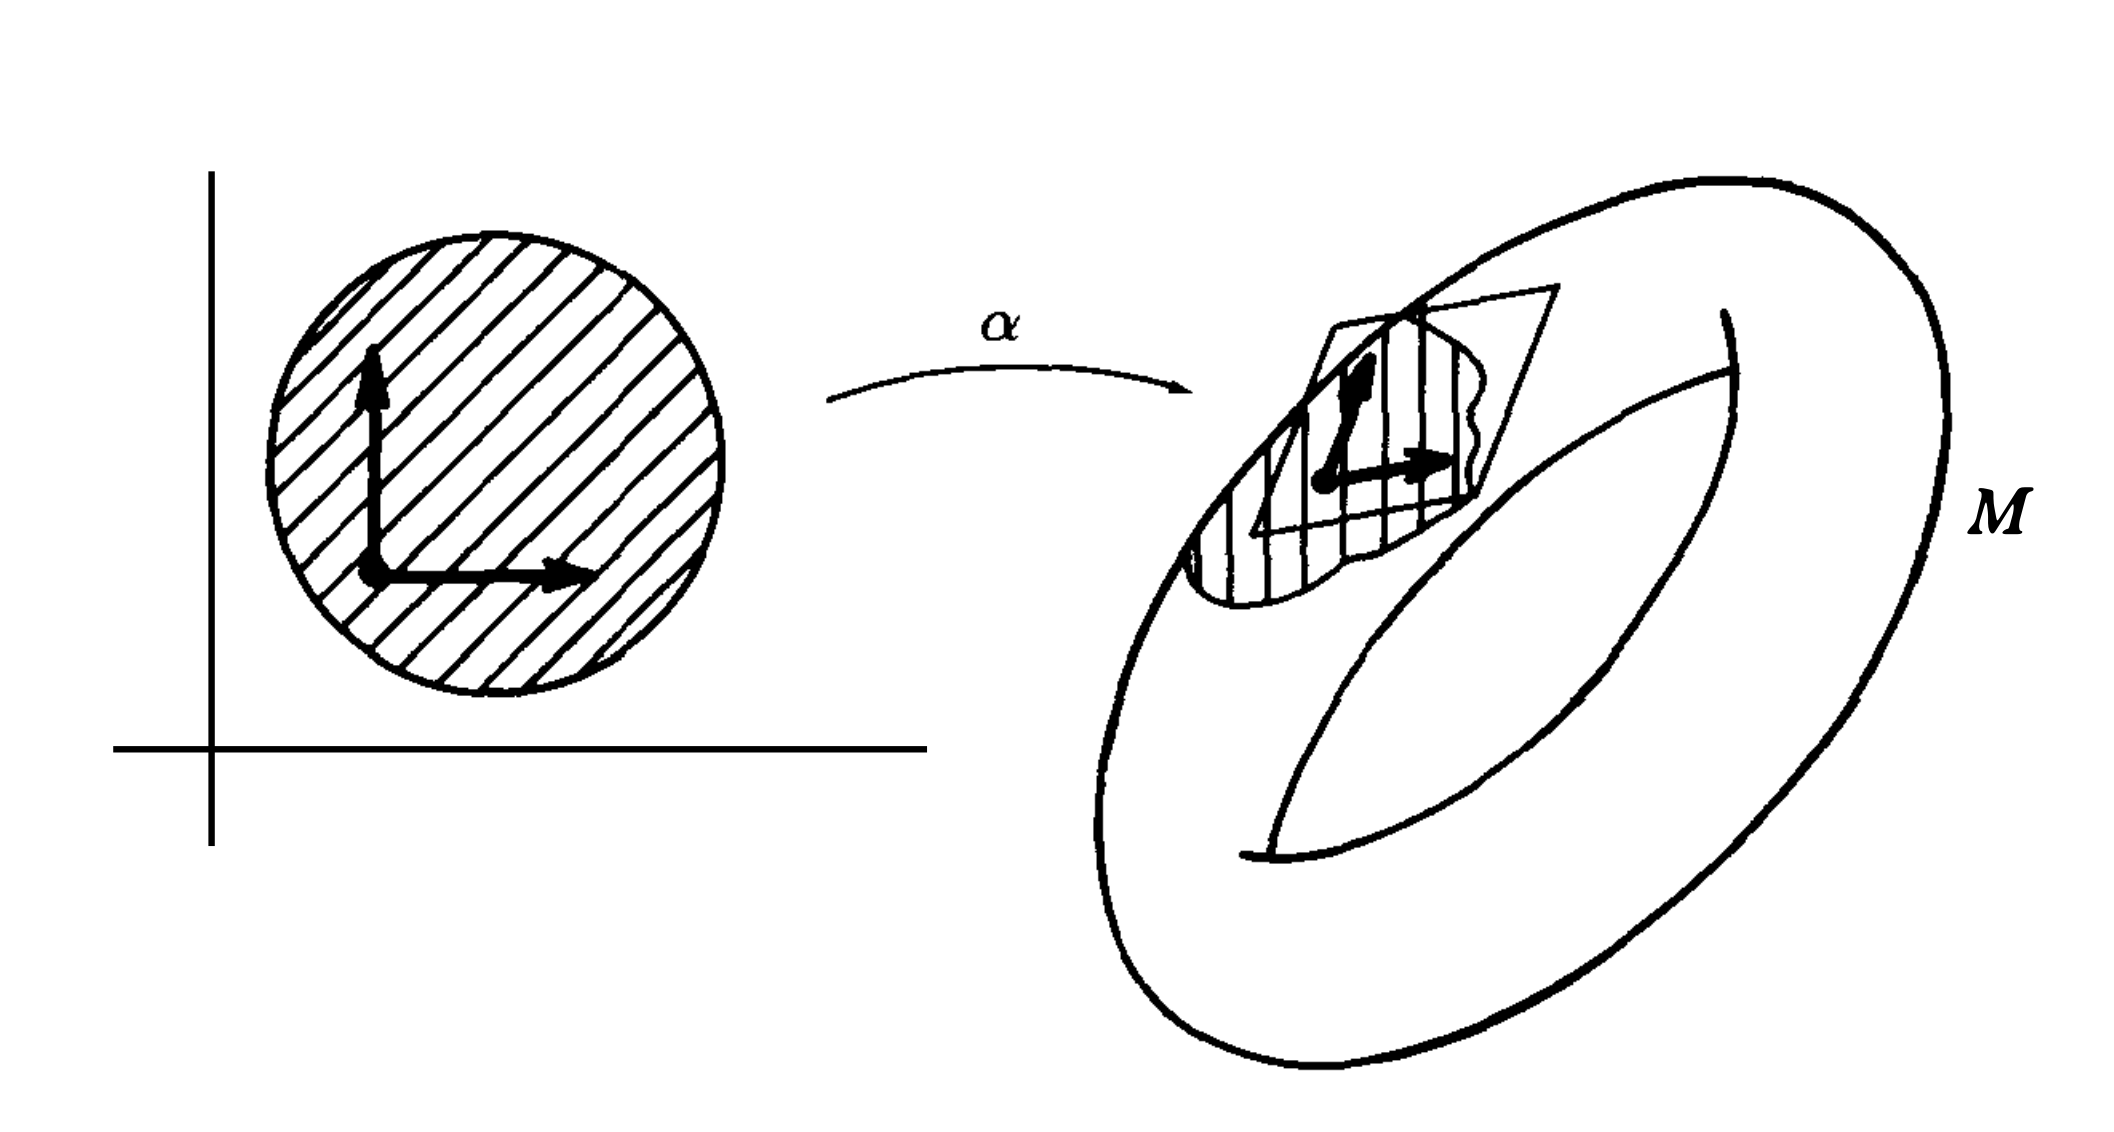
\includegraphics[scale=0.3]{images/Screenshot 2023-01-21 at 19.38.35.png}
        \caption{Meaning of $rank(D\alpha(x))=k$}
    \end{figure}
    Also, this condition means that $M$ does not have cusps or corners. This is a condition that parametrized
    -manifold does not have. 
    \item $\alpha^{-1}$ is continuous means that $\alpha:U\longrightarrow V$ should be a diffeomorphism.
    $M$ has the property that each point has a neighborhood that is homeomorphic(diffeomorphic) to an open subset of n-dimensional Euclidean space.
    While the parametrized-manifold only requirs parametrize the object with a continuous function.
\end{itemize}
\noindent \textbf{Examples}:(Non-examples for manifold without boundary)\\
\begin{itemize}
    \item Let $\alpha:\R\longrightarrow\R^2$ be given by the equation $$\alpha(t)=(t^3,t^2)$$
    Let $M$ be the image of $\R$. We can check that $M$ is a parametrized-manifold of dimension 1.
    \begin{figure}[H]
        \centering
        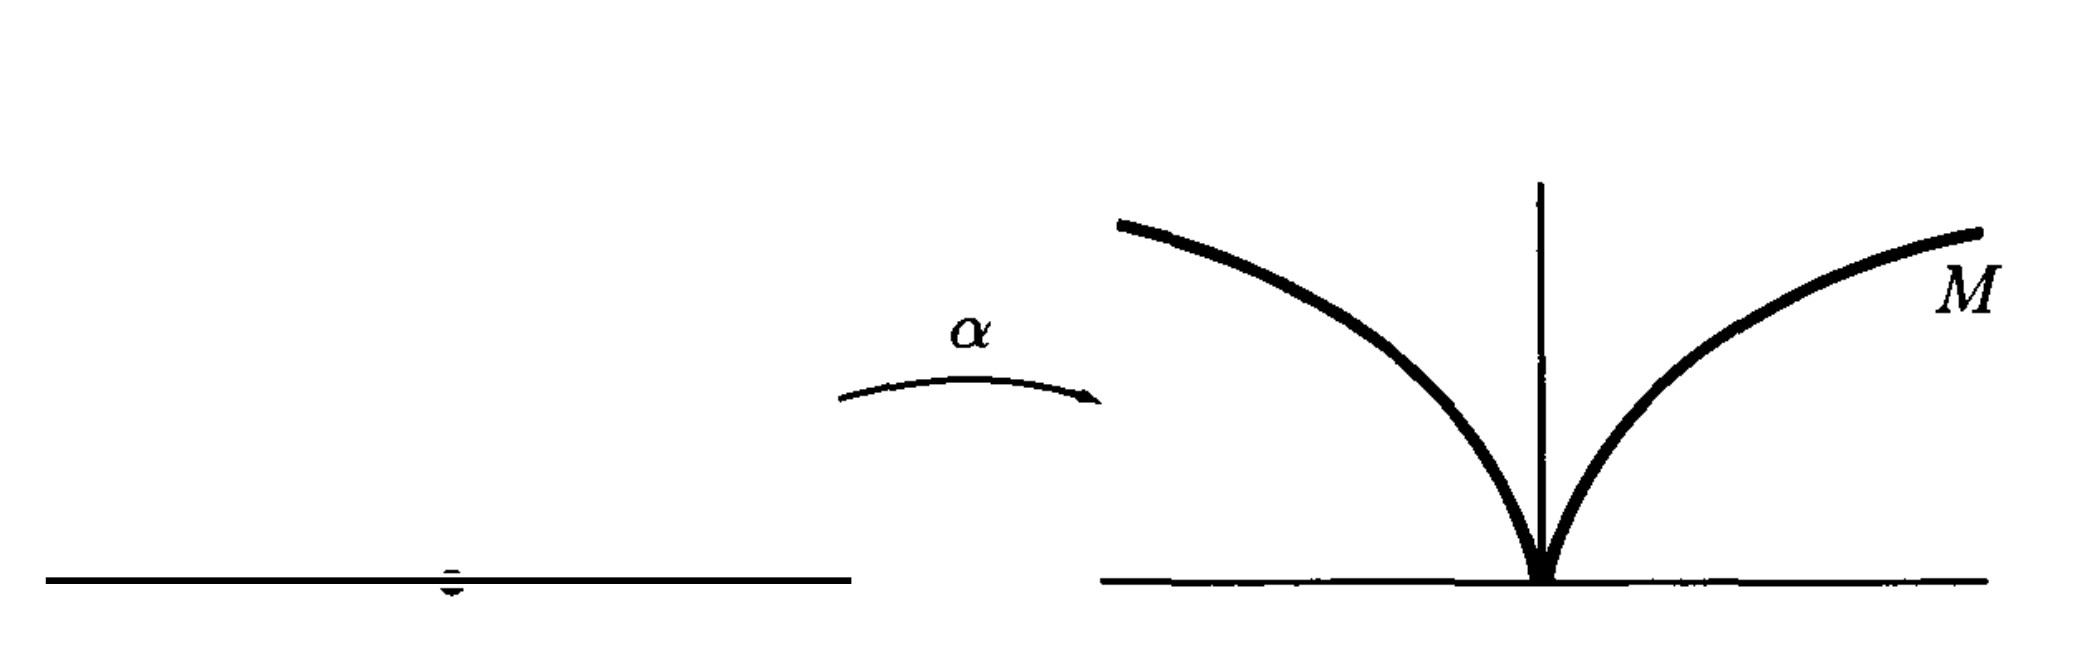
\includegraphics[scale=0.3]{images/Screenshot 2023-01-21 at 19.50.40.png}
        \caption{$\alpha(t)=(t^3,t^2)$}
    \end{figure}
    Also, $\alpha,\alpha^{-1}$ are continuous, $\alpha$ is of class $C^{\infty}$. But $rank(D\alpha(0))=0$, the picture shows that $M$ has a cusp at $0$. $M$ is not a manifold wihout boundary.
    
    \item Let $\alpha:\R^2\longrightarrow\R^3$ be given by the equation $$\alpha(x,y)=(x(x^2+y^2),y(x^2+y^2),x^2+y^2)$$
    Let $M$ be the image of $\R^2$. We can check that $M$ is a parametrized-manifold of dimension 2.
    \begin{figure}[H]
        \centering
        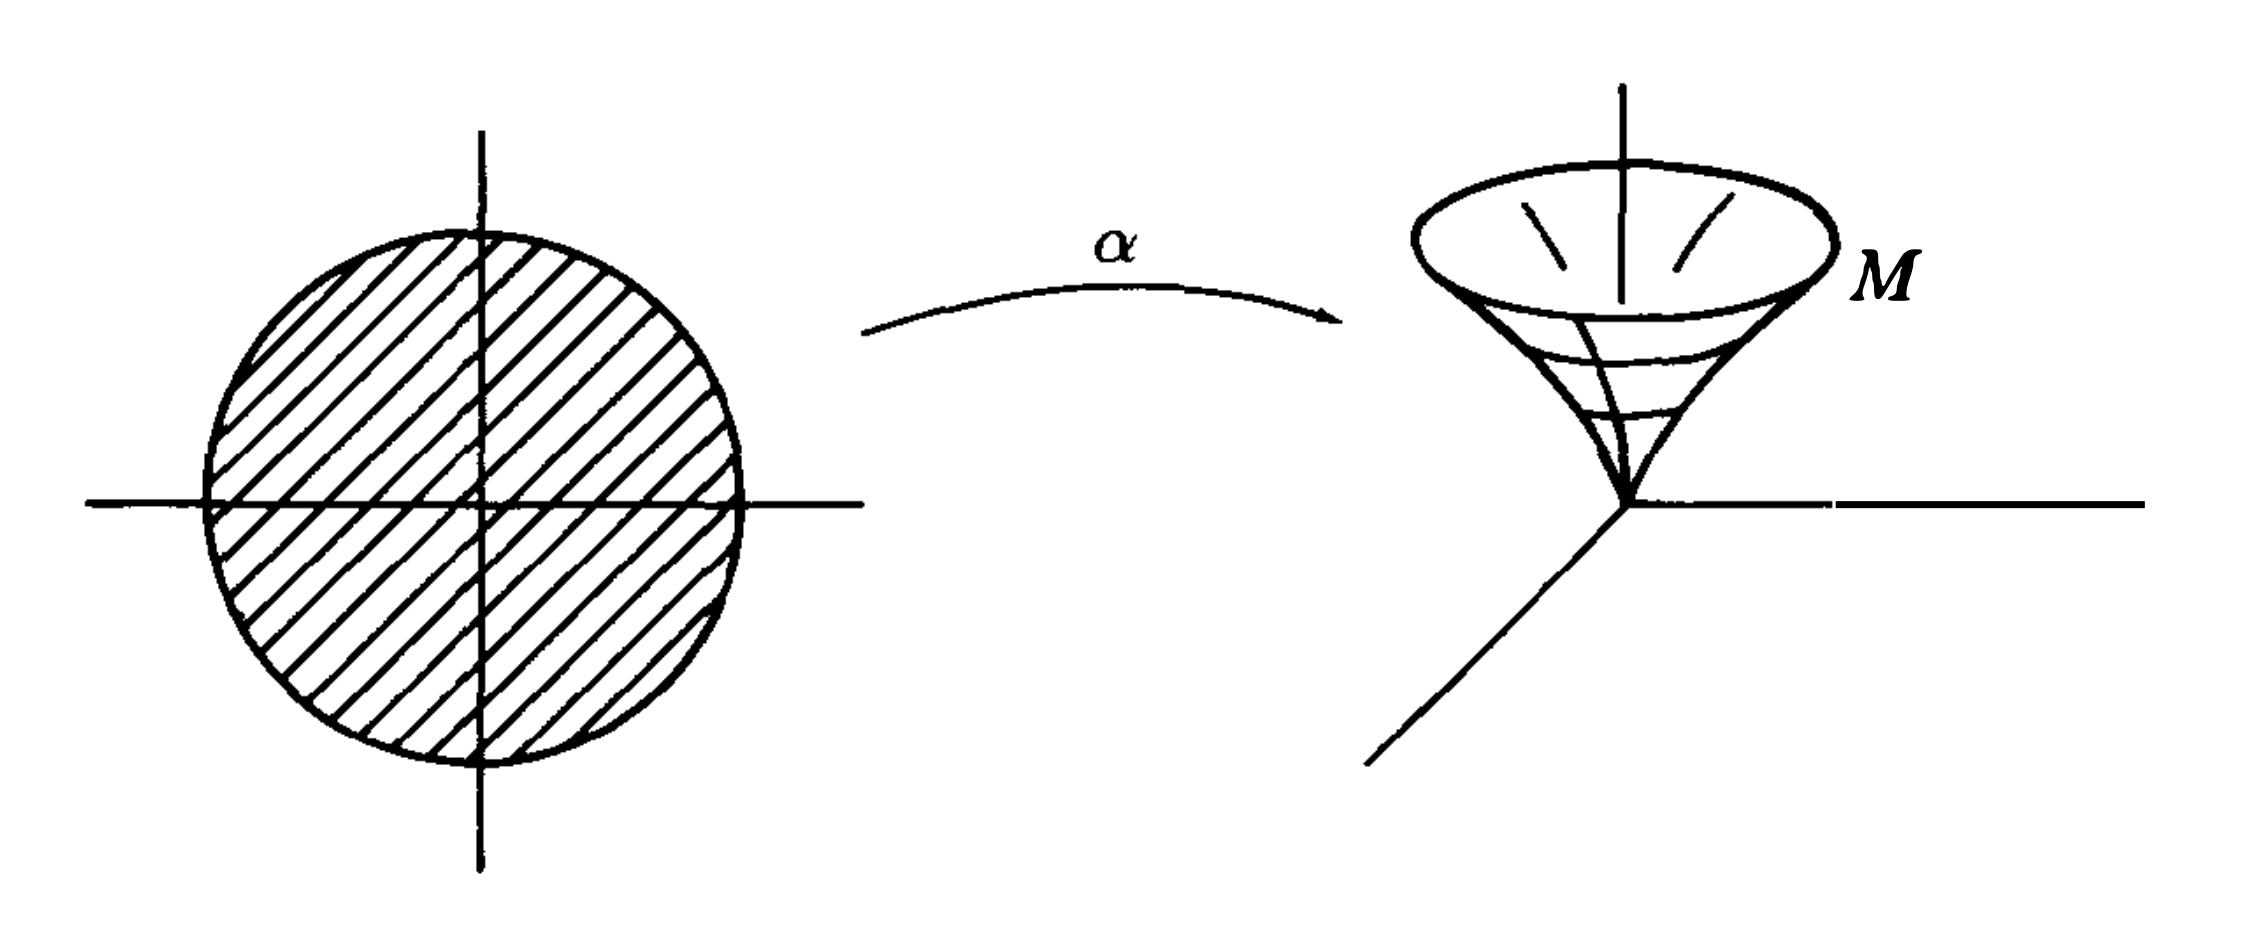
\includegraphics[scale=0.3]{images/Screenshot 2023-01-21 at 20.14.15.png}
        \caption{$\alpha(x,y)=(x(x^2+y^2),y(x^2+y^2),x^2+y^2)$}
    \end{figure}
    Also, $\alpha,\alpha^{-1}$ are continuous, $\alpha$ is of class $C^{\infty}$. But $rank(D\alpha(0))=0$, the picture shows that $M$ has a cusp at $0$. 
    In other words, $M$ fails to have a tangent plane at the origin. 
    $M$ is not a manifold wihout boundary.

    \item Let $\alpha:(0,\pi)\longrightarrow\R^2$ be given by the equation $$\alpha(t)=(\sin(2t)|\cos(t)|,\sin(2t)\sin(t))$$
    Let $M$ be the image of $(0,\pi)$. We can check that $M$ is a parametrized-manifold of dimension 1.
    \begin{figure}[H]
        \centering
        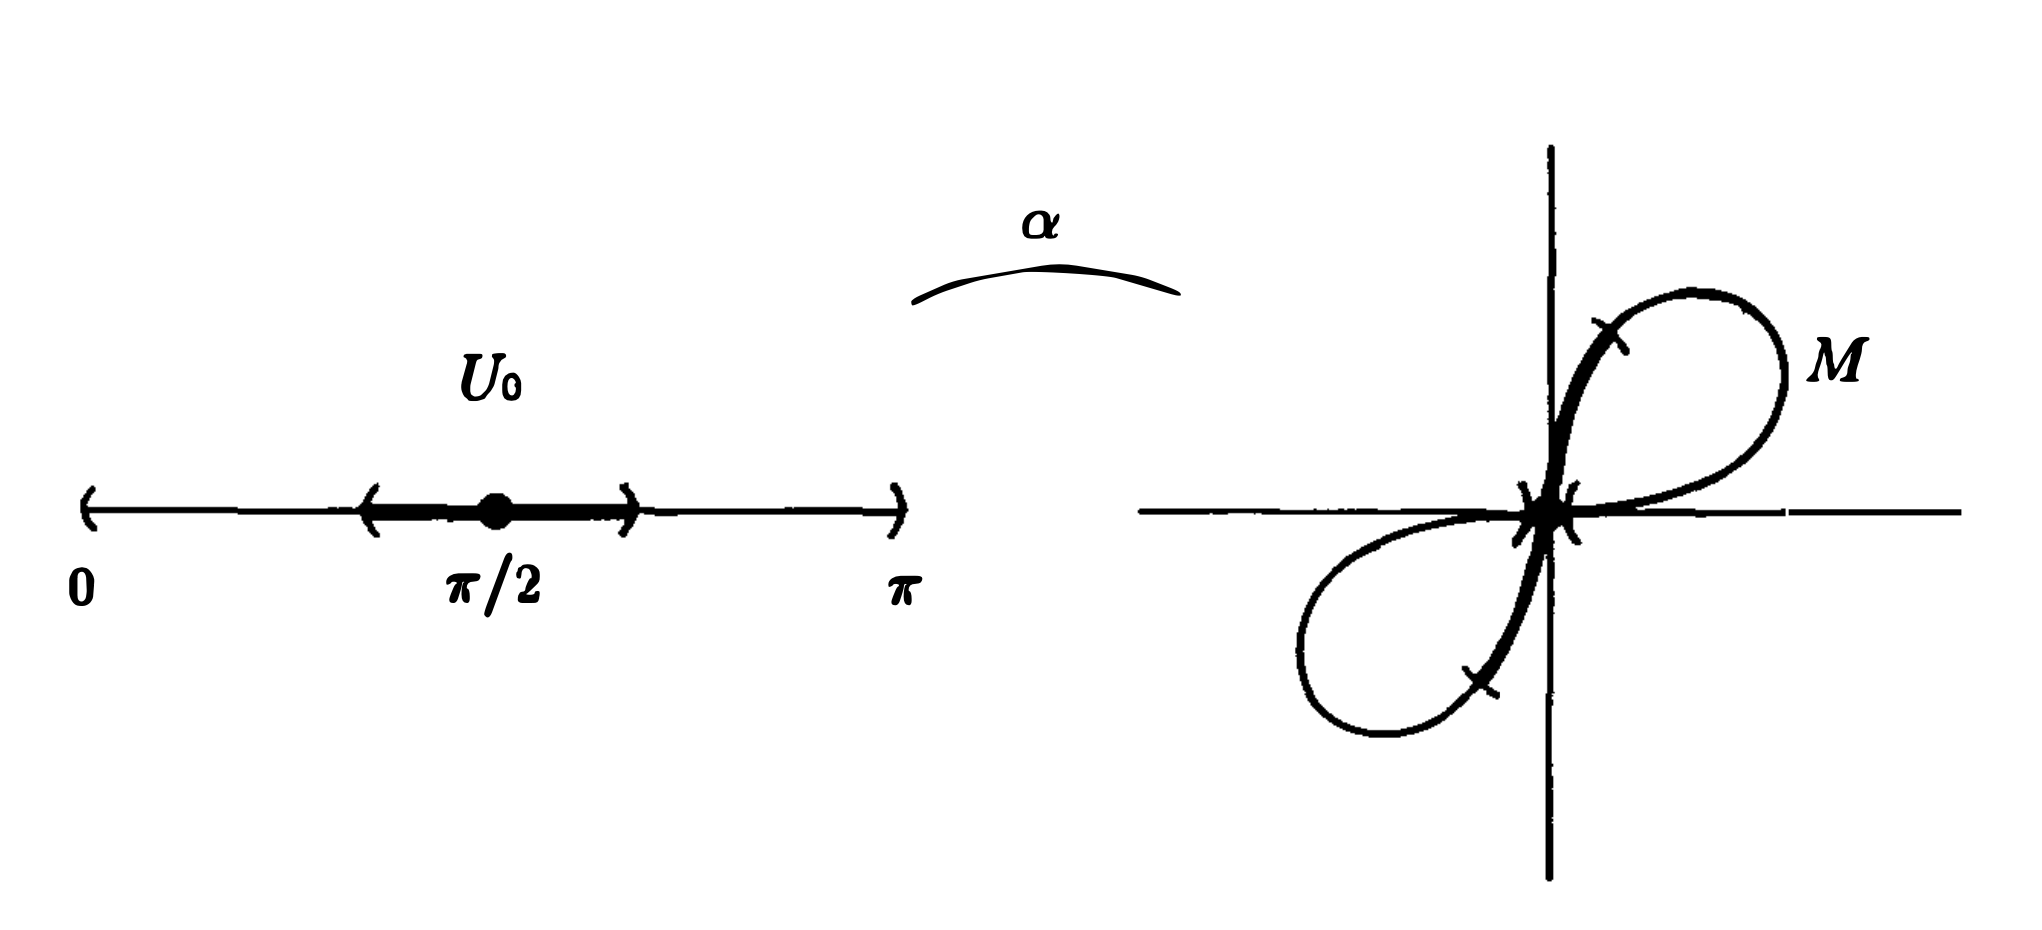
\includegraphics[scale=0.3]{images/Screenshot 2023-01-21 at 20.22.38.png}
        \caption{$\alpha(t)=(\sin(2t)|\cos(t)|,\sin(2t)\sin(t))$}
    \end{figure}
    This time, $\alpha$ is continuous and $rank(D\alpha)=1$ for all $x\in(0,\pi)$. But $\alpha^{-1}:M \longrightarrow(0,\pi)$ is not continuous.
    Let $U_0$ be an open set around $\frac{\pi}{2}$ in $(0,\pi)$ the preimage of $U_0$ under $\alpha^{-1}$ is not open in $M$.
\end{itemize}

\begin{theorem}
    Let $Y_{\alpha}$ be a parametrized-manifold with $\alpha:A\longrightarrow \R^n$. 
    If $\alpha^{-1}$ is continuous and $D\alpha$ has rank $k$, then $Y$ is a manifold without boundary. 
    In this case, $Y$ is covered by a single coordinate patch $\alpha$.
\end{theorem}

\begin{definition}
    Let $S$ be a subset of $\R^k$. Let $f:S\longrightarrow\R^n$. We say $f$ is \underline{of class $C^r$ on $S$} if $f$ may be extended to a function $g:U\longrightarrow\R^n$ that is of class $C^r$ on an open set $U$ of $\R^k$ containing $S$.
\end{definition}

\begin{theorem}
    By adopting the definition above, the composition of functions of class $C^r$ is of class $C^r$.
\end{theorem}

\begin{lemma}
    Let $f:S\subset\R^k\longrightarrow\R^n$. If for each $x\in S$, there is a neighborhood $U_x$ of $x$ such that $f|_{U_x\cap S}$ is of class $C^r$ on $U_x\cap S$, then $f$ is of class $C^r$ on $S$.
\end{lemma}

\begin{definition}\
    \begin{itemize}
        \item Let $\HH^k$ denote the \underline{upper half-space} in $\R^k$, consisting of those $x\in \R^k$ with $x_k\geq 0$.
        \item Let $\HH^k_+$ denote the \underline{open upper half-space} in $\R^k$, consisting of those $x\in \R^k$ with $x_k> 0$.
    \end{itemize}
\end{definition}
\noindent\textbf{Remark}:
\begin{itemize}
    \item We shall be particularly interested in functions defined on sets that are open in $\HH^k$ but not in $\R^k$.
\end{itemize}

\begin{lemma}
    Let $U$ be open in $\HH^k$. Let $\alpha:U\longrightarrow\R^n$ be of class $C^r$. Let $\beta:U'\longrightarrow\R^n$ be of class $C^r$ be an extension of $\alpha$ defined on an open set $U'\subset \R^k$. 
    Then $$\forall x\in U.D\beta(x)=D\alpha(x)$$
\end{lemma}

\begin{definition}
    Let $k > 0$. A \underline{k-manifold} in $\R^n$ of class $C^r$ is a subspace $M\subset \R^n$ having the following property:
    For each $p \in M$, there is an open set $V \subset M$ containing $p$, a set $U\subset \R^k$ that is either open in $\R^k$ or $\HH^k$, and a continuous bijective map $\alpha: U \longrightarrow V$ such that:
    \begin{itemize}
        \item $\alpha$ is of class $C^r$.
        \item $\alpha^{-1}:V \longrightarrow U$ is continuous.
        \item $D\alpha(x)$ has rank $k$ for each $x \in U$.
    \end{itemize}
    The map $\alpha$ is called a \underline{coordinate patch} on $M$ about $p$.
\end{definition}
\noindent\textbf{Remark}:
\begin{itemize}
    \item We extend the definition to the case $k=0$ by declaring a discrete collection of points in $\R^n$ to be a \underline{0-manifold} in $\R^n$.
    \item The difference of this definition and the definition of manifold without boundary is the set $U$ can be open in $\HH^k$. So the points which have neighborhoods that look like open half-balls in $\HH^k$ instead of open balls in $\R^k$ shall called the boundary of $M$. Consider the following picture.
    \begin{figure}[H]
        \centering
        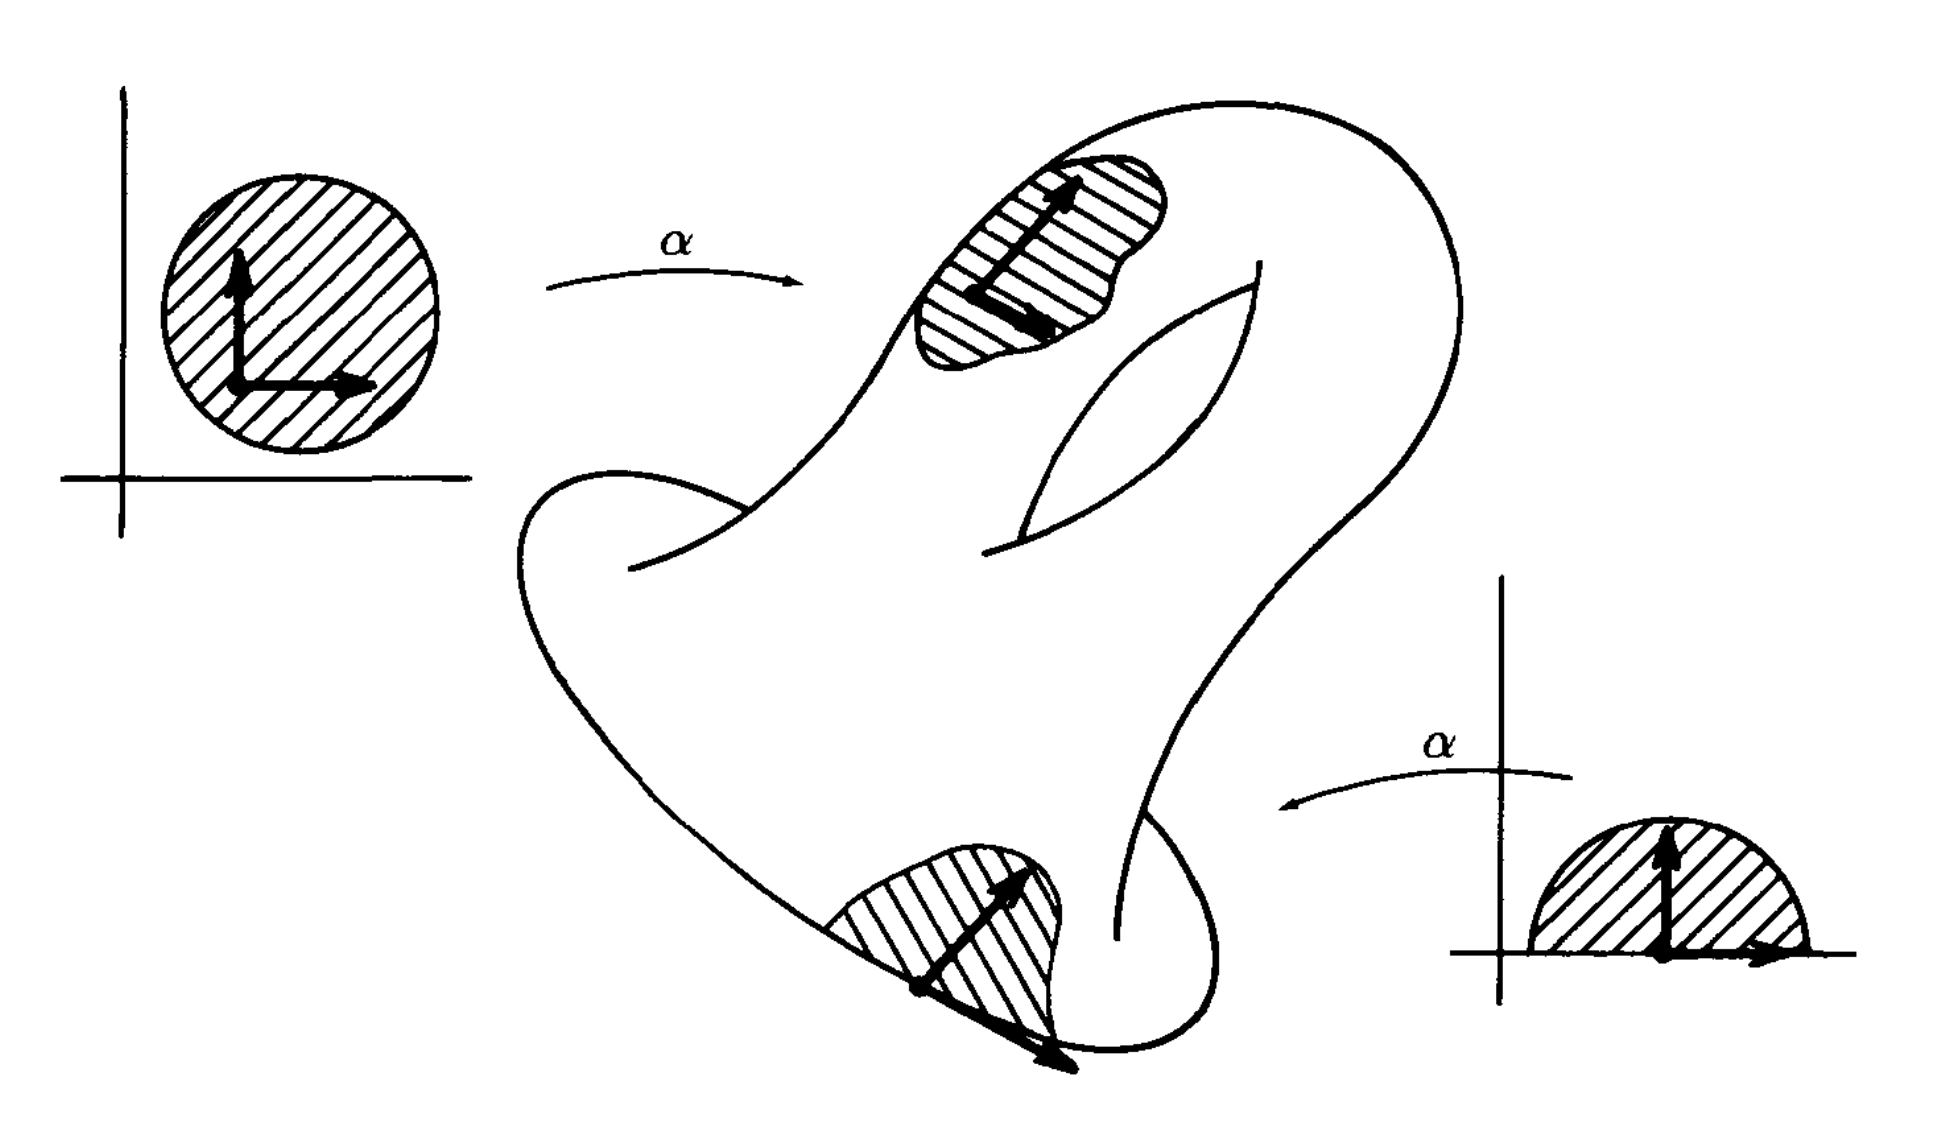
\includegraphics[scale=0.3]{images/Screenshot 2023-01-21 at 21.38.04.png}
        \caption{A picture of 2-manifold in $\R^3$}
    \end{figure}
    We will make this definition rigorous in the next section.
\end{itemize}

\begin{lemma}
    Let $M$ be a manifold in $\R^n$. Let $\alpha:U\longrightarrow V$ be a coordinate patch on $M$. If $U_0$ is a subset of $U$ that is open in $U$, then the restriction of $\alpha$ to $U_0$ is also a coordinate patch on $M$.
\end{lemma}

\section{The Boundary of a Manifold}

\begin{theorem}\label{transition function thm}
    Let $M$ be a k-manifold in $\R^n$ of class $C^r$. Given two coordinate patches $$\alpha_0:U_o\longrightarrow V_0$$ $$\alpha_1:U_1\longrightarrow V_1$$
    with the intersection $W=V_0\cap V_1\neq \emptyset$. Let $W_i=\alpha_i^{-1}(W)$. Then the map $$\alpha_1^{-1}\circ \alpha_0:W_0\longrightarrow W_1$$
    is of class $C^r$, and its derivative is non-singular. We call the function $\alpha_1^{-1}\circ \alpha_0$ \underline{transition function}.
\end{theorem}

\noindent\textbf{Remark}:
\begin{itemize}
    \item Since the sets $U_i$ are open in $\R^k$ or $\HH^k$. So we have three types of transitions as shown in the graph.
    \begin{figure}[H]
        \centering
        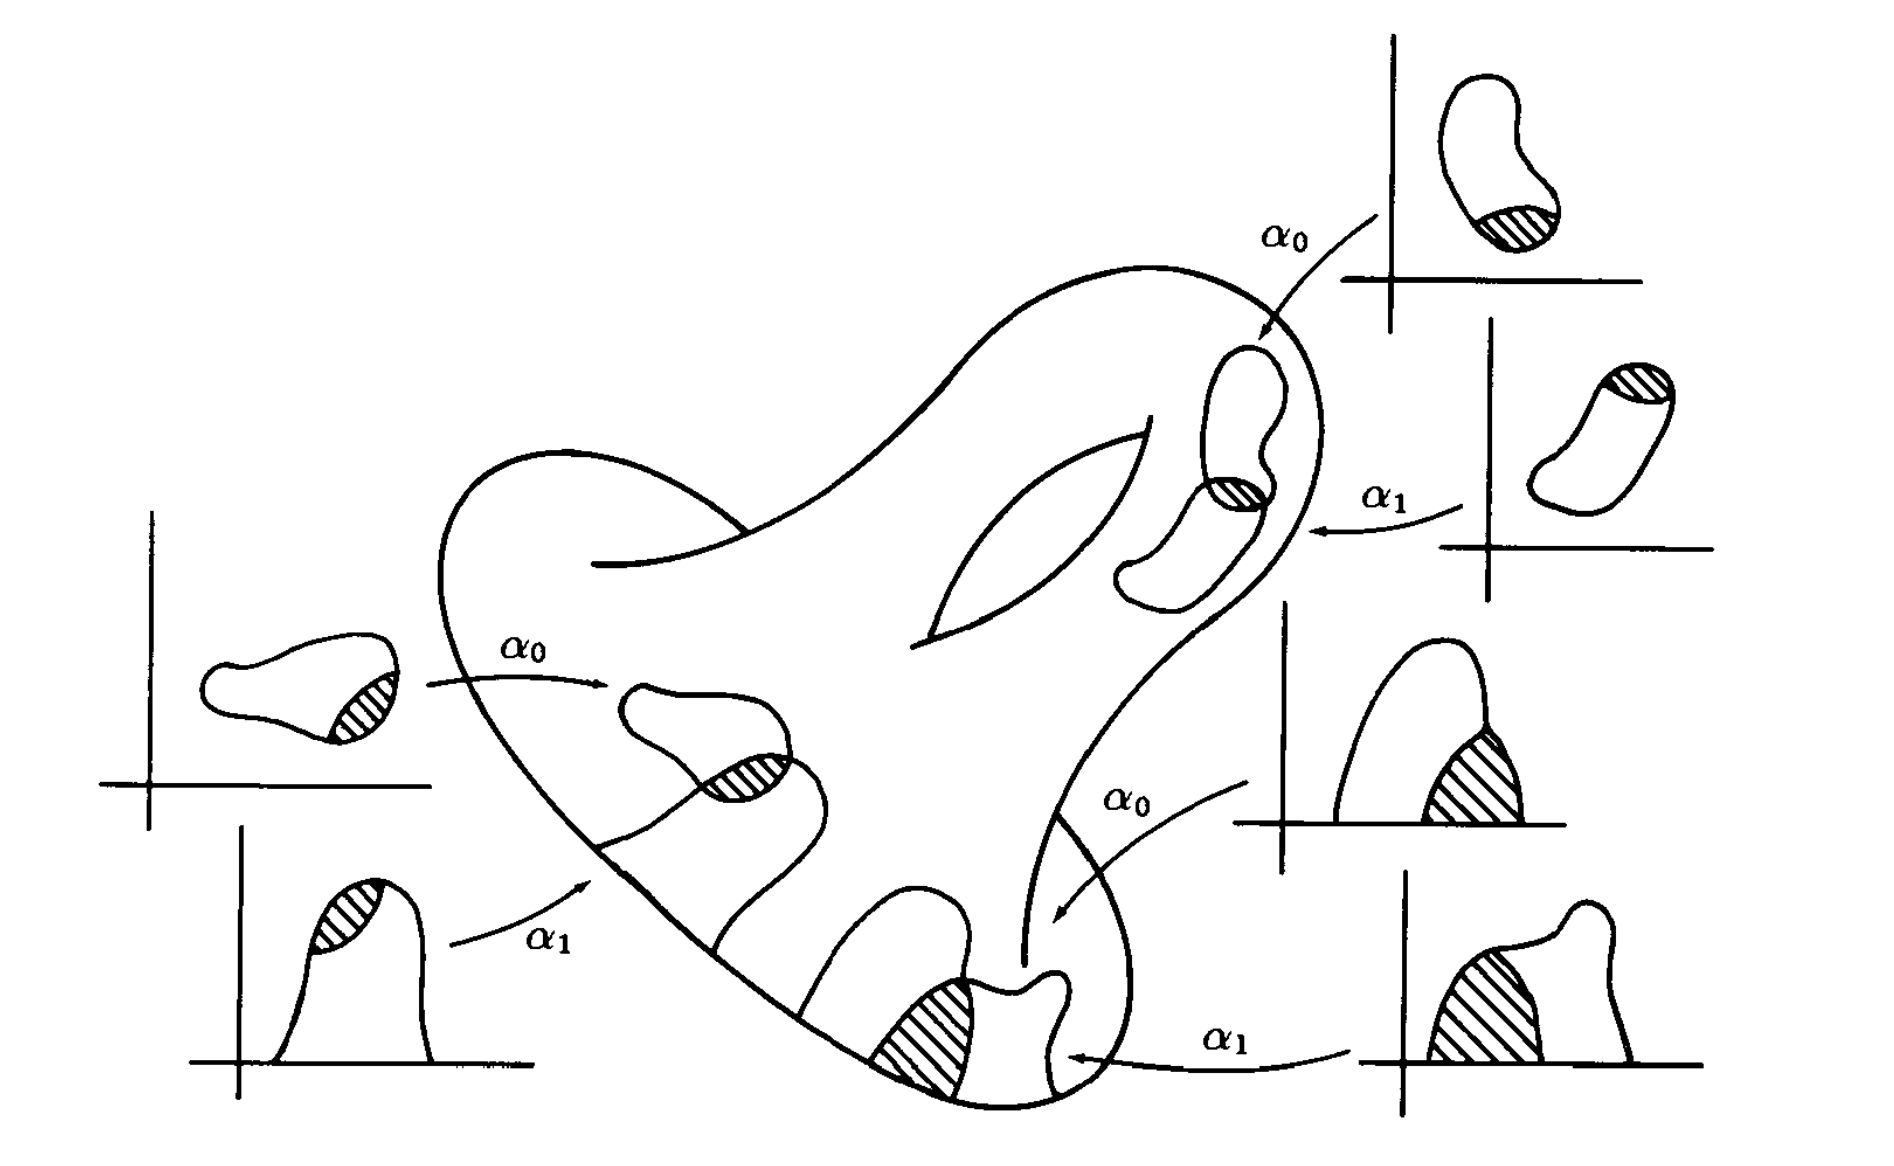
\includegraphics[scale=0.35]{images/Screenshot 2023-01-30 at 15.07.28.png}
        \caption{Three types of transition functions}
    \end{figure}
    \item In the future, we will study the manifold that does not live in $\R^n$, and this theorem will be very important to define such manifold.
\end{itemize}

\begin{definition}
    Let $M$ be a k-manifold in $\R^n$. Let $p\in M$.
    \begin{itemize}
        \item If there exists a coordinate patch $\alpha:U\longrightarrow V$ on $M$ about $p$ such that $U$ is open in $\R^k$, we say $p$ is an \underline{interior point} of $M$.
        \item If not, we say $p$ is a \underline{boundary point} of $M$. 
    \end{itemize}
    We denote the set of boundary points of $M$ by $\partial M$, and call this set the \underline{boundary} of $M$. 
\end{definition}
\noindent\textbf{Remark}:
\begin{itemize}
    \item The interior points and boundary points of the manifold $M$ has nothing to do with the term interior and boundary in general topology.
    \item Consider the $S^2$ in $\R^3$, all points in $S^2$ are interior points of the manifold $S^2$. But it is clear that $Int(S^2)=\emptyset$ because for any $p\in S^2.$ we cannot find any open ball of $x$ contained in $S^2$, hence all points in $S^2$ are in the boundary of $S^2$.
\end{itemize}

\begin{lemma}[Identify boundary points]
    Let $M$ be a k-manifold. Let $\alpha:U\longrightarrow V$ be a coordinate patch about the point $p\in M$.
    \begin{itemize}
        \item If $U$ is open in $\R^k$, then $p$ is an interior point.
        \item If $U$ is open in $\HH^k$ and $p=\alpha(x_0)$ for $x_0\in \HH^k_+$, then $p$ is an interior of $M$.
        \item If $U$ is open in $\HH^k$ and $p=\alpha(x_0)$ for $x_0\in \R^{k-1}\times 0$, then $p$ is a boundary point of $M$.
    \end{itemize}
\end{lemma}

\begin{theorem}
    Let $M$ be a k-manifold in $\R^n$ of class $C^r$. If $\partial M$ is non-empty, then $\partial M$ is a k-1 manifold without boundary in $\R^n$ of class $C^r$.
\end{theorem}

\begin{theorem}
    Let $\mathcal{O}$ be open in $\R^n$. Let $f:\mathcal{O}\longrightarrow \R$ be of class $C^r$. 
    Let $M$ be the set of points $x$ for which $f(x)=0$. Let $N$ be the set of points for which $f(x)\geq0$. 
    Suppose $M$ is non-empty and $\forall x \in M.rank(Df(x))=1$. Then $N$ is an n-manifold in $\R^n$ and $\partial N=M$.
\end{theorem}
\noindent\textbf{Example}:
\begin{itemize}
    \item The n-ball $B^n(a)$ is an n-manifold in $\R^n$ of class $C^{\infty}$ and $\partial B^n(a)=S^{n-1}(a)$ which is the (n-1)-sphere.\\ 
    We apply the preceding theorem to the function $$f(x)=a^2-\norm{x}^2=a^2-(x_1)^2-\cdots-(x_n)^2$$
    Hence we can compute the derivative of $f$ $$Df(x)=\begin{bmatrix}
        (-2x_1) & \cdots & (-2x_n)
    \end{bmatrix}$$
    This matrix has rank 1 at each points of $S^{n-1}(a)$.
    \item The  solid torus $T$ is a 3-manifold, and its boundary is the torus.\\
    Let $g$ be the cylindrical coordinate transformation. Let $$A=\{(r,\theta,z):(r-b)^2+z^2\leq a^2\text{ and }0\leq \theta\leq 2\pi\}$$
    Recall the previous example, the \underline{Solid Torus} $T$ is the image of $A$ under $g$. We define $f:\R^3\longrightarrow\R$ as $$f(x,y,x)=a^2-(\sqrt{x^2+y^2}-b)^2-z^2$$
    Intuitively, $f$ is the square of the distance of point $(x,y,z)$ to the torus $\partial T$. By computation, 
    $$Df(x,y,z)=\begin{bmatrix}
        -2x+\frac{2xb}{\sqrt{x^2+y^2}}& -2y+\frac{2yb}{\sqrt{x^2+y^2}}&-2z
    \end{bmatrix}$$
    We need to show that $rank(Df(x,y,z))=1$ whenever $f(x,y,z)=0$. This is equivalent to proving the contrapositive statement: 
    $$rank(Df(x,y,z))\neq1\implies f(x,y,z)\neq0$$
    Suppose $rank(Df(x,y,z))\neq1$, then it must be 0. Hence $x^2+y^2=b^2$ and $z=0$. Therefore $f(x,y,z)=a^2>0$.
\end{itemize}

\begin{theorem}
    Let $f:\R^{n+k}\longrightarrow\R^n$ be of class $C^r$. Let $M=\{x\in \R^{n+k}:f(x)=0\}$. Suppose $M$ is non-empty and $\forall x\in M.rank(Df(x))=n$, then we have
    \begin{enumerate}
        \item $M$ is a k-manifold without boundart in $\R^{n+k}$.
        \item If $N=\{x\in\R^{n+k}:f_1(x)=\cdots=f_{n-1}(x)\text{ and }f_n(x)\geq 0\}$ and $$\forall x \in N.rank(D(f_1,\cdots,f_{n-1})(x))=n-1$$
        Then $N$ is a (k+1)-manifold and $\partial N=M$.
    \end{enumerate}
\end{theorem}
\noindent\textbf{Remark}:
\begin{itemize}
    \item The solution of the equation $f(x)=(f_1(x),\cdots,f_n(x))=\vec{0}$ can be thought as the intersection of hyper-surfaces $f_i(x)=0$. If the condition of the theorem above is satisfied, then $f_1(x)=0$ is a (n+k-1)-manifold, when it intersects $f_2(x)=0$, the dimension will minuse 1. After intersects $f_n(x)=0$, we intersects $n-1$ times, Hence $M$ has dimension $n+k-1-(n-1)=k$.
    \item for example, let $f,g:\R^3\longrightarrow\R$ be of class $C^r$. Let $M\neq \emptyset$ be the solution set of the system of equations \begin{equation*}
        \begin{cases}
            f(x,y,z)=0\\
            g(x,y,z)=0
        \end{cases}
    \end{equation*}
    Define $h=(f,g):\R^3\longrightarrow\R^2$. If we have the condition that $$\forall x\in M.rank(Dh(x))=2$$
    Then $M$ is a 1-manifold without boundary in $\R^3$. In other words, the solution set is a smooth curve without singularities.
\end{itemize}

\section{Integral of Scalar Functions over Manifold}

\begin{definition}
    Let $M$ be a compact k-manifold in $\R^n$ of class $C^r$. Let $f:M\longrightarrow\R^n$ be a continuous function. Let $C=supp(f)$. $C$ is compact beacause $C$ is closed in compact space $M$. Suppose $C$ can be covered by a single coordinate patch. i.e. $$\exists \text{ coordinate patch }\alpha:U\longrightarrow V.\text{such that }C\subset V$$
    Now $\alpha^{-1}(C)$ is compact in $\R^k$. Therefore, by replacing $U$ by a smaller open set if necessary, we can assume that $U$ is bounded. we define the \underline{integral of $f$ over $M$} by 
    $$\int_Mf\di V=\int_{Int(U)}(f\circ \alpha)V(D\alpha)$$
    \begin{itemize}
        \item If $U$ is open in $\R^k$, then $Int(U)=U$.
        \item If $U$ is open in $\HH^k$ but not open in $\R^k$, then $Int(U)=U\cap\HH^k_+$.
    \end{itemize}
\end{definition}
\noindent\textbf{Remark}:
\begin{itemize}
    \item The function $F=(f\circ\alpha)V(D\alpha)$ is continuous on bounded $U$ and vanish outside the compact set $\alpha^{-1}(C)$, hence $F$ is bounded.
    If $U$ is open in $\R^k$ , then $F$ vanishes near each point of $Bd(U)$. If $U$ is not open in $\R^k$, then $F$ vanishes near near each point of $Bd(U)$ not in $\partial \HH^k$. In either case, 
    $F$ is integrable over $U$ and hence over $Int(U)$.
    \begin{figure}[H]
        \centering
        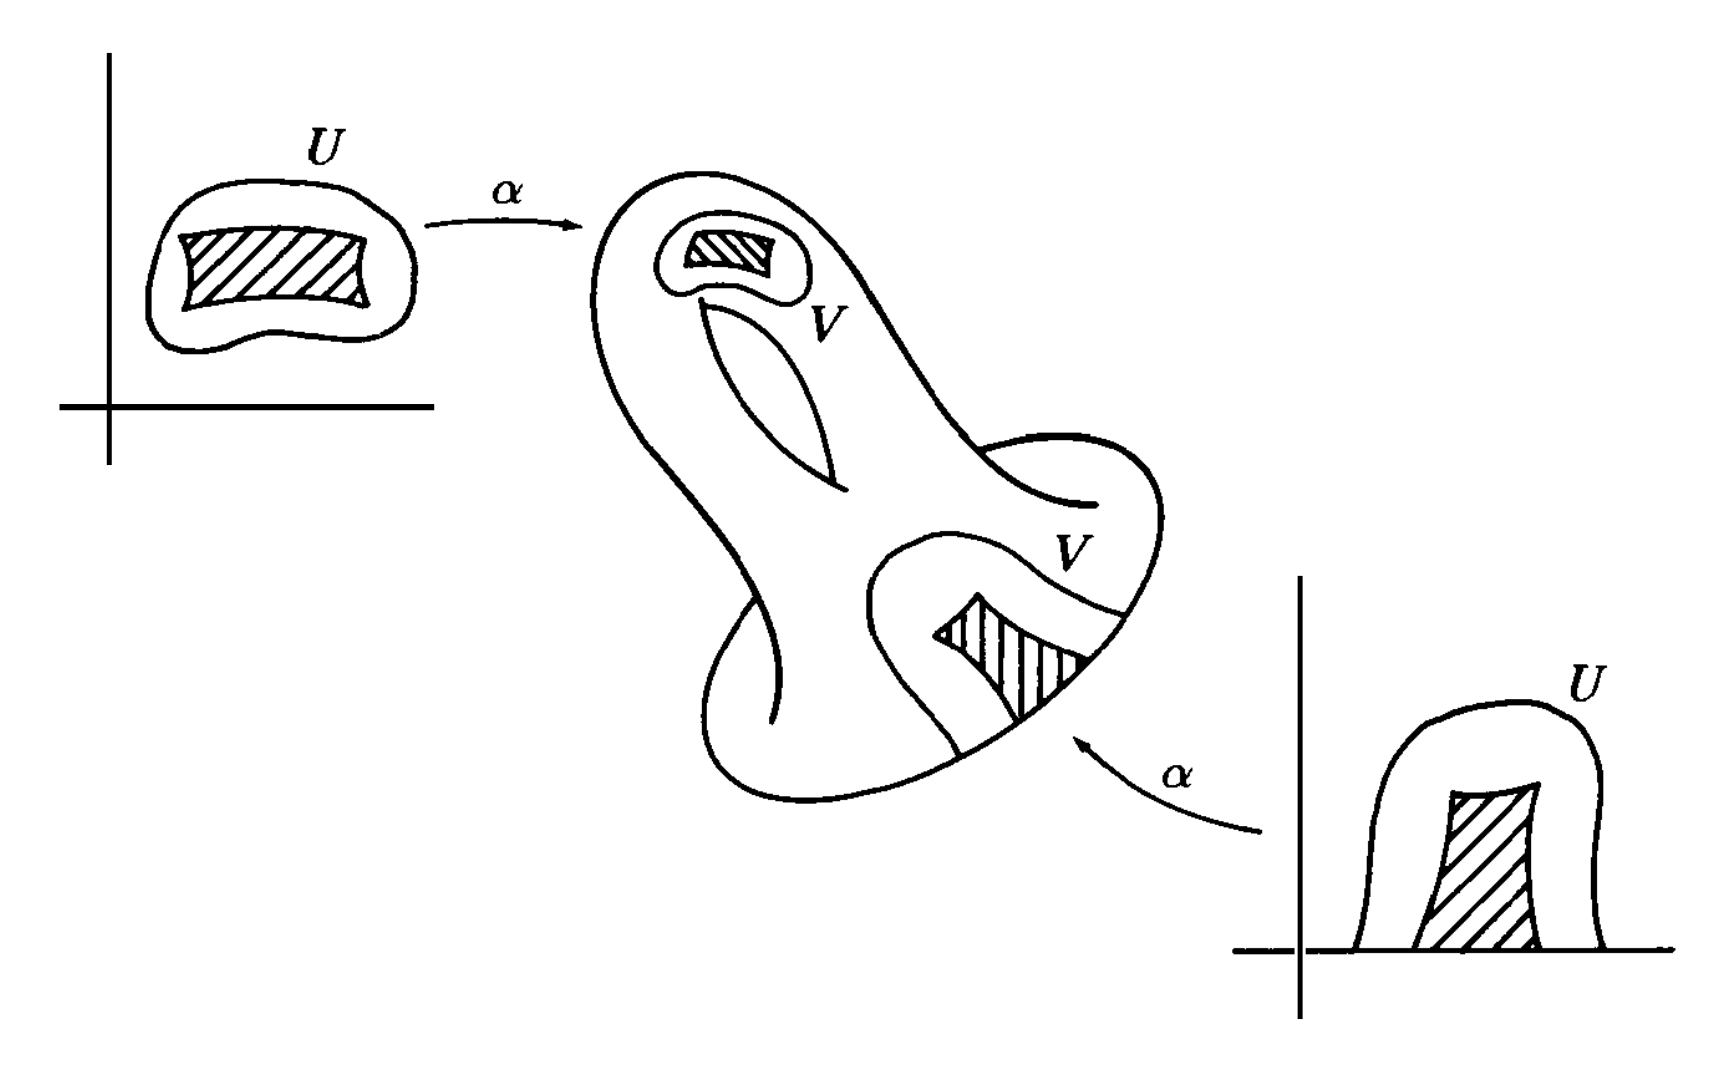
\includegraphics[scale=0.3]{images/Screenshot 2023-02-07 at 22.27.15.png}
    \end{figure}
    \item This integral exists as an ordinary integral, and hence as an extended integral.
\end{itemize}

\begin{lemma}
    If the support of $f$ can be covered by a single coordinate patch, the integral $\int_Mf\di V$ is well-defined, independent of the choice of coordinate patch.
\end{lemma}

\begin{theorem}[existence of finite partition of unity on $M$]
    Let $M$ be a compact k-manifold in $\R^n$ of class $C^r$. Given a covering of $M$ by coordinate patches, there exists a finite collection of $C^{\infty}$ functions $\phi_1,\cdots,\phi_l:\R^n\longrightarrow[0,1]$ such that
    \begin{enumerate}
        \item Given $i$, the support of $\phi_i$ is compact and there is a coordinate patch $\alpha_i:U_i\longrightarrow V_i$ belonging to the given covering such that $$(supp(\phi_i)\cap M)\subset V_i$$
        \item $\sum\phi_i(x)=1$ for $x\in M$.
    \end{enumerate}
    We call $\{\phi_1,\cdots,\phi_l\}$ a \underline{partition of unity on $M$} dominated by the given collecction of coordinate patches. 
\end{theorem}

\begin{definition}
    Let $M$ be a compact k-manifold in $\R^n$ of class $C^r$. Let $f:M\longrightarrow \R$ be continuous. 
    Choose a partition of unity $\{\phi_1,\cdots,\phi_l\}$ on $M$ that is dominated by the collection of all coordinate patches on $M$. 
    We define the \underline{inegral of $f$ over $M$} by the equation 
    $$\int_Mf\di V=\sum_{i=1}^l[\int_M(\phi_if)\di V]$$
    Then we define the \underline{k-dimensional volume of $M$} by the equation 
    $$v(M)=\int_M1\di V$$
\end{definition}
\noindent\textbf{Remark}:
\begin{itemize}
    \item Clearly, this is a more general definition. If the support of $f$ happens to lie in a single coordinate patch $\alpha:U\longrightarrow supp(f)\subset V$, this definition agrees with the preceding definition.
    \begin{equation*}
        \begin{split}
            \sum_{i=1}^l[\int_M(\phi_if)\di V] &= \sum_{i=1}^l[\int_{Int(U)}(\phi_if\circ \alpha)V(D\alpha)] \text{\quad by definition}\\
            &= \int_{Int(U)}[\sum_{i=1}^l(\phi_if\circ \alpha)V(D\alpha)] \text{\quad by linearity}\\
            &= \int_{Int(U)}[\sum_{i=1}^l(\phi_i\circ \alpha)(f\circ \alpha)V(D\alpha)]\\
            &= \int_{Int(U)}(f\circ\alpha)V(D\alpha)\text{\quad because\quad} \sum_{i=1}^l(\phi_i\circ\alpha)=1 \text{ on $A$}\\
            &= \int_Mf\di V \text{\quad by definition}
        \end{split}
    \end{equation*}
    \item What if $supp(f)$ is not contained in a single coordinate patch? Suppose $supp(f)$ is contained in $\{\alpha_1,\cdots,\alpha_t\}$ where $\alpha_i:U_i\longrightarrow V_i$.
    \begin{itemize}
        \item For $\alpha_1:U_1\longrightarrow V_1$, we keep it unchanged. Set $U_1'=U_1,V_1'=V_1$.
        \item For $\alpha_2$, we restrict it as $\alpha_2\big|^{V_2\setminus V_1}$, say $\alpha_2:U_2'\longrightarrow V_2'$.
        \item For $\alpha_k$, we restrict it as $\alpha_k\big|^{V_k\setminus V_{k-1}'}$, say $\alpha_2:U_k'\longrightarrow V_k'$.
    \end{itemize}
    After this process, we get $\{V_1'\cdots,V_t'\}$, which is a partition of $supp(f)$.For each part $V_k'$ of the manifold $M$, with similar argument we get
    $$\sum_{i=1}^l[\int_{V_k'}(\phi_if)\di V]=\int_{V_k'}f\di V$$
    Therefore we have 
    \begin{equation*}
        \begin{split}
            \sum_{i=1}^l[\int_M(\phi_if)\di V] &= \sum_{i=1}^l\sum_{k=1}^t[\int_{V_k'}(\phi_if)\di V]\\
            &= \sum_{k=1}^t\sum_{i=1}^l[\int_{V_k'}(\phi_if)\di V]\\
            &= \sum_{k=1}^t\int_{V_k'}f\di V\\
            &= \int_Mf\di V
        \end{split}
    \end{equation*}
    \item Also notice that this definition is independent of the choice of the partition of unity. Let $\{\psi_1,\cdots,\psi_m\}$ be another choice for the partition of unity. 
    Since $$supp(\psi_jf)\subset supp(\psi_j)\cap supp(f)\subset supp(\psi_j)\cap M\subset V_j$$ where $\psi_j:U_j\longrightarrow V_j$ this means that the support of $\psi_jf$ lies in a single coordinate patch. With similar argument (replacing $f$ by $\psi_jf$) we have 
    $$\sum_{i=1}^l[\int_M(\phi_i\psi_jf)\di V]=\int_M(\psi_jf)\di V$$ 
    Summing over $j$ we get 
    \begin{equation*}
        \begin{split}
            \sum_{j=1}^m\sum_{i=1}^l[\int_M(\phi_i\psi_jf)\di V] &= \sum_{j=1}^m\int_M(\psi_jf)\di V\\
            &= \int_Mf\di V\\
            &= \sum_{i=1}^l[\int_M(\phi_if)\di V]
        \end{split}
    \end{equation*}
\end{itemize}

\begin{theorem}
    Let $M$ be a compact k-manifold in $\R^n$ of class $C^r$. Let $f,g:M\longrightarrow \R$ be continuous. Then 
    $$\int_M(af+bg)\di V =a \int_M f\di V + b\int_M g \di V$$
\end{theorem}
\noindent\textbf{Remark}:
\begin{itemize}
    \item Using partition of unity to define the integral of $f$ over compact manifold $M$ is satisfactory for theoretical purposes, but not for practical purposes. 
    \item For example, if we want to integrate a function over $S^{n-1}$, no one want to actually find a partition of unity on $S^{n-1}$. Instead, we break $S^{n-1}$ into pieces and integrate over each pieces separatelt then add the results together.
\end{itemize}

\begin{definition}
    Let $M$ be a compact k-manifold in $\R^n$ of class $C^r$. A subset $D\subset M$ is said to have \underline{measure zero in $M$} if $D$ can be covered by countably many coordinate patches $\alpha_i:U_i\longrightarrow V_i$ such that the set $$D_i=\alpha_i^{-1}(D\cap V_i)$$ has measure zero in $\R^k$ for each $i$. 
\end{definition}

\begin{theorem}[Equivalent definition of measure zero in $M$]
    $D\subset M$ has measure zero in compact k-manifold $M$ if and only if for any coordinate patch $\alpha:U\longrightarrow V$ on $M$, the set $\alpha^{-1}(D\cap V)$ has measure zero in $\R^k$.
\end{theorem}

\begin{theorem}
    Let $M$ be a compact k-manifold in $\R^n$ of class $C^r$. Let $f:M\longrightarrow \R$ be continuous. Suppose we have coordinate patches $\{\alpha_1,\cdots,\alpha_N\}$ where $\alpha_i:A_i\longrightarrow M_i$ such that $A_i$ is open in $\R^k$. Also, $\{M_1,\cdots,M_N,K\}$ is a partition of $M$ where $K$ has measure zero in $M$. Then
    $$\int_Mf\di V=\sum_{i=1}^N[\int_{A_i}(f\circ\alpha_i)V(D\alpha_i)]$$
\end{theorem}
\noindent\textbf{Remark}:
\begin{itemize}
    \item This theorem is for practical purposes. And it says that $\int_Mf\di V$ can be evaluated by breaking $M$ up into pieces that are parametrized-manifolds and integrating $f$ over each piece separately.
\end{itemize}
\noindent\textbf{Example}:
\begin{itemize}
    \item Alternate method for computing the area of $S^2(a)$.\\
    Recall that we think the upper hemisphere with radius $a$ as a parametrized-manifold and used improper integral to get the area of the upper hemisphere is $2\pi a^2$. Hence the area of $S^2(a)$ is $4\pi a^2$. 
    Given $z_0\in \R$ with $|z_0|<a$, the intersection of $S^2(a)$ with the plane $z=z_0$ is the circle 
    $$\{(x,y,z)\in S^2(a): x^2+y^2=a^2-(z_0)^2\text{ and }z=z_0\}$$
    This fact suggests that we parametrize $S^2(a)$ by the function $\alpha:A\longrightarrow \R^3$
    $$\alpha(t,z)=(\sqrt{a^2-z^2}\cos(t), \sqrt{a^2-z^2}\sin(t), z)$$
    where $A$ is the set 
    $$A=\{(t,z)\in \R^2: 0<t<2\pi \text{ and }|z|<a\}$$
    \begin{figure}[H]
        \centering
        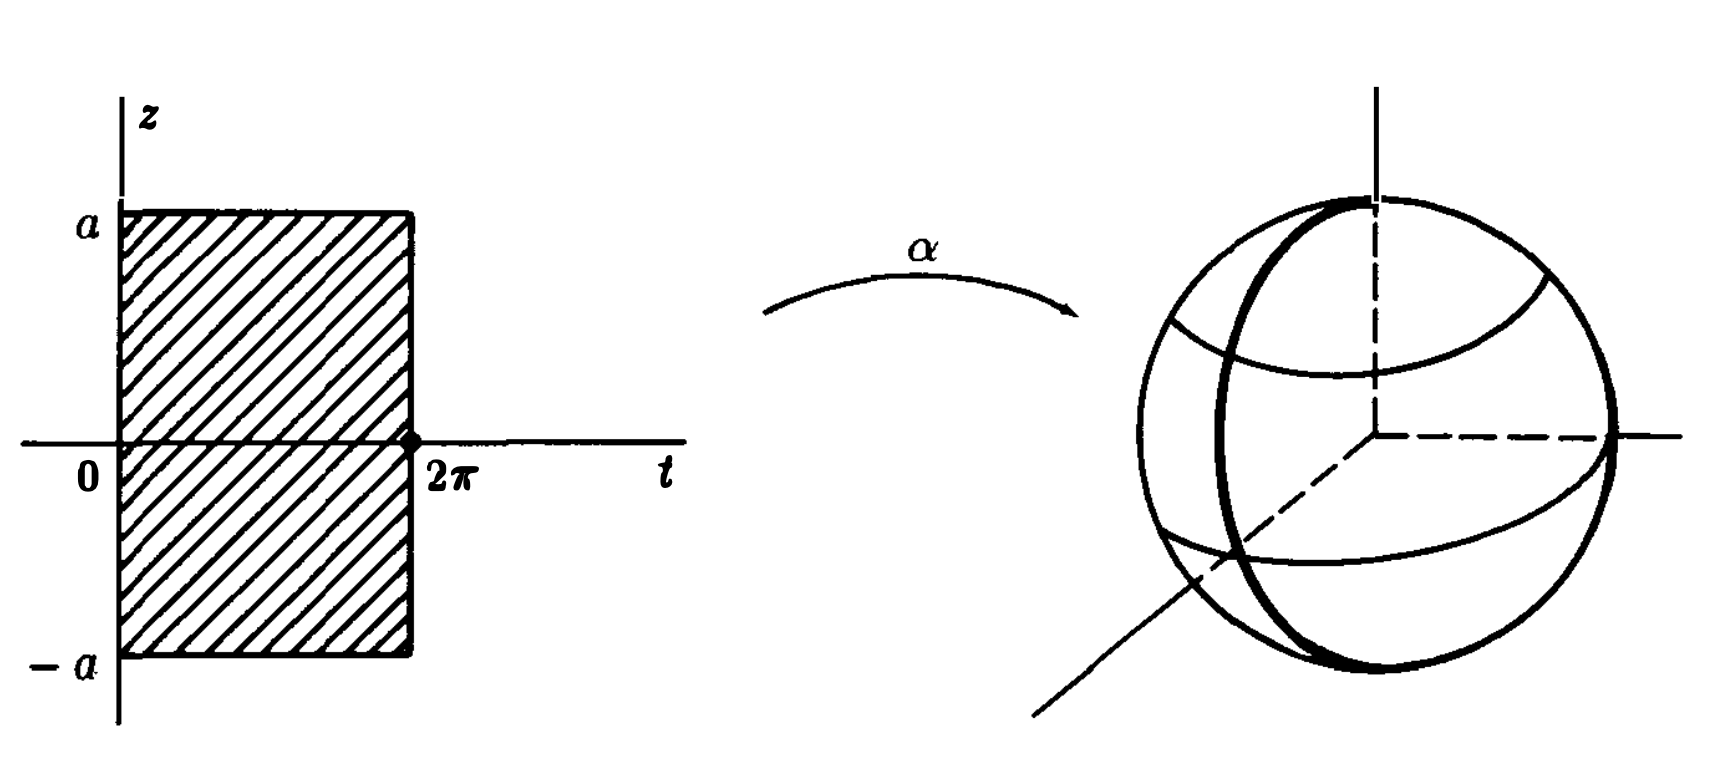
\includegraphics[scale=0.3]{images/Screenshot 2023-02-27 at 22.11.04.png}
    \end{figure}
    As shown in the picture that $\alpha$ is a coordinate patch that covers all of $S^2(a)$ except for a great-circle arc, which has measure zero in $S^2(a)$.
    Sicne \begin{equation*}
        D\alpha=\begin{bmatrix}
            -\sqrt{a^2-z^2}\sin(t) & \frac{-z\cos(t)}{\sqrt{a^2-z^2}}\\
            \sqrt{a^2-z^2}\cos(t) & \frac{-z\sin(t)}{\sqrt{a^2-z^2}}\\
            0 & 1
        \end{bmatrix}
    \end{equation*}
    By brutal computation we have $V(D\alpha)=\sqrt{\det(D^T\alpha\cdot D\alpha)}=a$, Therefore
    \begin{equation*}
        v(S^2(a))= \int_A1V(D\alpha)=\int_Aa=4\pi a^2
    \end{equation*}
\end{itemize}

\begin{theorem*}
    Let $M$ and $N$ be compact manifolds without boundary in $\R^m$ and $\R^n$ respectively. Let $f:M\longrightarrow \R$ and $g:N\longrightarrow \R$ be continuous. Then 
    $$\int_{M\times N}f\cdot g \di V=[\int_Mf\di V][\int_Ng\di V]$$
    It followa that $$v(M\times N)=v(M)\times v(N)$$
\end{theorem*}
\noindent\textbf{Example}:
\begin{itemize}
    \item In topology, we know that the torus is homeomorphic to $S^1\times S^1$. But what is $S^1\times S^1$? It is a 2-manifold in $\R^4$ and we can now compute the area of $S^1\times S^1$
    $$v(S^1\times S^1)=v(S^1)\times v(S^1)=(2\pi)^2$$
\end{itemize}
\include{differential Forms}
\chapter{Stokes' Theorem}

\section{Integrating Forms over Parametrized-Manifolds}
\begin{definition}
    Let $A$ be open in $\R^k$. Let $\eta$ be a k-form defined in $A$. Then $\eta$ can be written uniquely in the form 
    $$\eta =f\cdot dx_1\wedge \cdots \wedge dx_k$$
    We define the \underline{integral of $\eta$ over $A$} by the equation $$\int_A\eta=\int_Af$$
    provided that the latter integral exists.
\end{definition}
\noindent\textbf{Remark}:
\begin{itemize}
    \item Forms are more abstract, the integral of forms are even more abstract. But no worries, we will get some geometric intepretation later.
\end{itemize}

\begin{theorem}
    Let $\{a_1,\cdots,a_k\}$ be any right-handed orthonormal basis for $\R^k$, then we have 
    $$\int_A\eta=\int_{x\in A}\eta(x)((x;a_1),\cdots,(x;a_k))$$
\end{theorem}

\begin{definition}
    Let $A$ be open in $\R^k$. Let $\alpha:A\longrightarrow\R^n$ be of class $C^{\infty}$. 
    The set $Y=\alpha(A)$, together with the map $\alpha$, constitute the parametrized-manifold $Y_{\alpha}$. 
    Let $\omega$ be a k-form defined in an open set of $\R^n$ containing $Y$, we define the \underline{integral of $\omega$ over $Y_{\alpha}$} by the equation 
    $$\int_{Y_{\alpha}}\omega=\int_A\alpha^*\omega$$
    provided the latter exists. Since $\alpha^*$ and $\int_A$ are linear, so is this integral.
    $$\int_{Y_{\alpha}}(a\omega+b\eta)=a\int_{Y_{\alpha}}\omega+b\int_{Y_{\alpha}}\eta$$
\end{definition}

\begin{theorem}[Invariant under reparametrization]
    Let $g:A\longrightarrow B$ be a diffeomorphism of open sets in $\R^k$. 
    Assume $\det(Dg)$ does not change sign on $A$. 
    Let $\beta:B\longrightarrow\R^n$ be a map of class $C^{\infty}$. 
    Let $Y=\beta(B)$. Let $\alpha=\beta\circ g$, then $\alpha:A\longrightarrow\R^n$ and $Y=\alpha(A)$. 
    If $\omega$ is a k-form defined in an open set of $\R^n$ containing $Y$, then $\omega$ is integrable over $Y_{\beta}$ if and only if it is integrable over $Y_{\alpha}$. In this case 
    $$\int_{Y_{\alpha}}\omega=\pm \int_{Y_{\beta}}\omega$$
    where the sign agrees with the sign of $\det(Dg)$.
\end{theorem}
\noindent\textbf{Remark}:
\begin{itemize}
    \item If $A$ is connected, then the hypothesis that $\det(Dg)$ does not change sign on $A$ is automatically satisfied.
\end{itemize}

\begin{theorem}
    Let $A$ be open in $\R^k$. Let $\alpha:A\longrightarrow\R^n$ be of class $C^{\infty}$. 
    Let $Y=\alpha(A)$. Let $x$ denote the general point of $A$ and $z$ denote the general point of $\R^n$. If $$\omega=f\cdot dz_I$$
    is a k-form defined in an open set of $\R^n$ containing $Y$, then $$\int_{Y_{\alpha}}\omega=\int_A(f\circ \alpha)\det(\frac{\partial \alpha_I}{\partial x})$$
\end{theorem}

\noindent\textbf{Remark}:
\begin{itemize}
    \item Recall in single-variable calculus. Let $A=(a,b)$ an open interval. Then $$\int_Afdx=\int_a^bf$$
    where the notation $fdx$ on the left denotes the integral of a 1-form and the notation on the right denotes the integral of a function.
\end{itemize}

\section{Orientable Manifolds}

\subsection{Definition of Orientation of Manifolds}

\begin{definition}
    The \underline{support of a differential form}, including a k-form $\omega$, is a concept from the field of differential geometry that describes the region where the form is non-zero. In more precise terms, the support of a k-form $\omega$, denoted as $supp(\omega)$, is the closure of the set of points in the k-manifold $M$ where the form does not vanish:
    $$supp(\omega)=\overline{\{p\in M: \omega(p)\neq 0}\}$$
\end{definition}

\noindent\textbf{Remark}:
\begin{itemize}
    \item To say that $\omega(p)$ does not vanish at a point $p$ means that it is not the zero tensor at that point. In other words, there exists a set of k linearly independent tangent vectors at point $p$ such that the k-tensor $\omega(p)$ evaluated on these vectors is non-zero:
    $$\omega(p)((p;v_1),\cdots,(p;v_k))\neq 0$$
    \item We will define the integral of a k-form $\omega$ over k-manifold $M$ in much the same way that we define the integral of a scalar function over $M$. first we treat the case where the support of $\omega$ lies in a single coordinate patch $\alpha:U\longrightarrow V$. in this case we define
    $$\int_M\omega=\int_{Int(U)}\alpha^*\omega$$
    However, if we change the parametrization of the manifold (i.e., change the coordinate system or the way the manifold is described), the integral's value may change in sign but not in magnitude.
    \item In order to make this well defined, we need an extra condition on $M$, called orientability.
\end{itemize}

\begin{definition}
    In previous section, we defined what is orientation-preserving for linear transformation $h\in \mathcal{L}(\R^k,\R^k)$. 
    We now generalize this to diffeomorphism $g:A\longrightarrow B$ of open sets in $\R^k$.
    \begin{itemize}
        \item We say that $g$ is \underline{orientation-preserving} if $\det(Dg)>0$ on $A$.
        \item We say that $g$ is \underline{orientation-reversing} if $\det(Dg)<0$ on $A$.
    \end{itemize}
\end{definition}

\begin{theorem*}
    Given diffeomorphism $g$, for each point $x\in A$, we have an induced linear transformation on tangent spaces $$g_*:\mathcal{T}_x(\R^k)\longrightarrow\mathcal{T}_{g(x)}(\R^k)$$
    The diffeomorphism $g$ is orientation-preserving if and only if $g_*$ is orientation-preserving in the linear transformation sense for each $x\in A$.
\end{theorem*}

\begin{definition}
    Let $M$ be a k-manifold in $\R^n$. Given coordinate pathches $$\alpha_0:U_0\longrightarrow V_0$$
    $$\alpha_1:U_1\longrightarrow V_1$$
    We say two coordinate pathces \underline{overlap} if $V_0\cap V_1\neq \emptyset$. 
    We say they \underline{overlap positively} if the transition function $$\alpha_1^{-1}\circ \alpha_0:W_0\subset \R^k\longrightarrow W_1$$
    is orientation-preserving.
\end{definition}

\begin{definition}
    If $M$ can be covered by coordinate pathces (also called atlas or charts) $\{(U_i,\alpha_i)\}$ that each pair of which overlap positively(if they overlap), then $M$ is said to be \underline{orientable}. 
    Otherwise, $M$ is said to be \underline{non-orientable}.
\end{definition}

\begin{definition}
    Suppose $M$ is orientable. Given two collection of coordinate pathces $\{(U_i,\alpha_i)\}_{i\in I}$ and $\{(U_j,\alpha_j)\}_{j\in J}$, we can show the union of them is also overlap positively. 
    We put all possible collection of such coordinate patches together, this is called an \underline{orientation} on $M$. 
    A manifold $M$ together with an orientation is called an \underline{oriented manifold}.
\end{definition}
\noindent\textbf{Remark}:
\begin{itemize}
    \item A k-manifold($k\geq1$) can have different orientations. But for 0-manifold, which is a collection of discrete points, this definition makes no sense, we will discuss the orientation of 0-manifold later.
    \item Let $\R^k$ be a vector space of dimension $k$, then $\R^k$ is also a k-manifold. We now have two notions of orientation of $\R^k$. 
    \begin{itemize}
        \item For $\R^k$ as a vector space, it has two orientations. One is the collection of all right-handed k-frames and the other is the collection of all left-handed k-frames.
        \item For $\R^k$ as a k-manifold, it still has two orentations that corresponds to the above two. The connection is easy to describe. Given an orientation of $\R^k$ in the sense of vector space, we can pick a k-frame $(v_1,\cdots,v_k)$. The linear isomorphism $\alpha:\R^k\longrightarrow\R^k$ such that $\alpha(e_i)=v_i$ is a coordinate patch on $\R^k$. And we can check that two coordinate pathces overlap positively.
    \end{itemize}
\end{itemize}

\subsection{Oriented Manifolds in $\R^n$ of Specific Dimension}

\begin{definition}
    Let $M$ be an oriented 1-manifold in $\R^n$. We define a corresponding unit tangent vector field $$T:M\longrightarrow\mathcal{T}(M)$$
    as follows: Given $p\in M$, choose a coordinate patch $\alpha:U\longrightarrow V$ on $M$ about $p$ belonging to the given orientation, we define $$T(p)=(p;\frac{D\alpha(t_0)}{\norm{D\alpha(t_0)}})$$
    where $t_0$ is the parameter value such that $\alpha(t_0)=p$.\\
    Then $T$ is called the \underline{unit tangent field corresponding to the orientation of $M$}.
\end{definition}

\noindent\textbf{Remark}:
\begin{itemize}
    \item The unit tangent field $T$ is the geometric interpretation of the orientation of a 1-manifold.
\end{itemize}

\begin{definition}
    In the case of a 1-manifold $M$, we shall allow the domains of coordinate patches on $M$ to be open sets in $\R^1$ or in $\HH^1$ or in $\mathbb{L}^1$. Where $$\mathbb{L}^1=(-\infty,0]$$
    We will explain why we add $\mathbb{L}^1$ in the following examples.
\end{definition}

\noindent\textbf{Example}:
\begin{itemize}
    \item Given an oriented 1-manifold $M$ without boundary, with corresponding unit tangent field $T$. $M$ has some kind of circular structure, although it can has knots but we do not care here, see the following picture. 
    We often picture the direction of $T$ by drawing an arrow on the curve $M$ itself. 
    \begin{figure}[H]
        \centering
        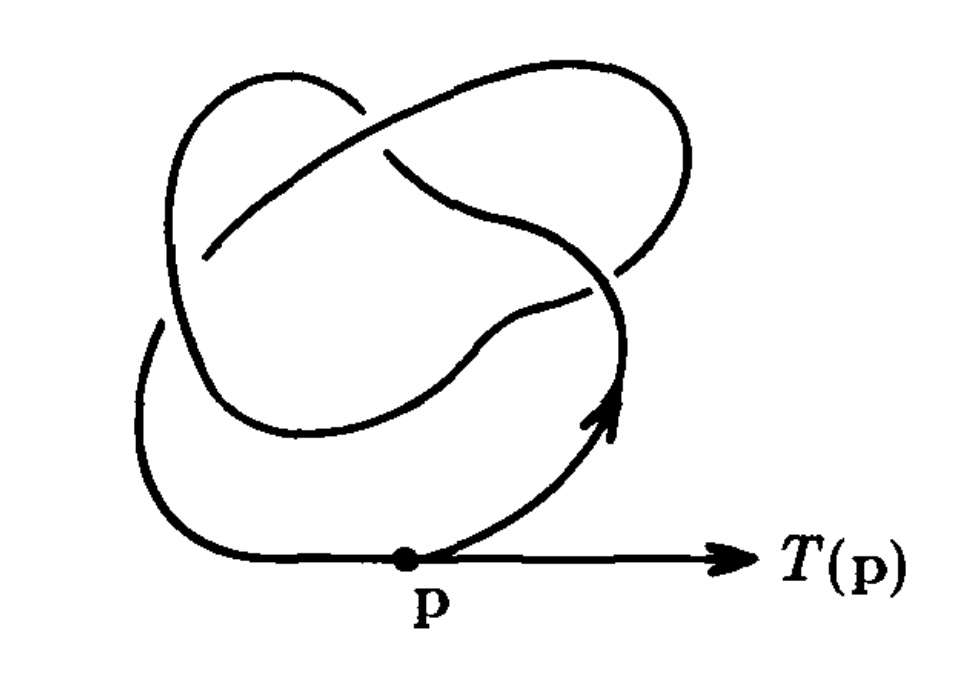
\includegraphics[scale=0.3]{images/Screenshot 2023-04-01 at 17.55.10.png}
    \end{figure}
    \item Now consider an oriented 1-manifold $M$ that has boundary. For the 1-manifomd in the picture, $\partial M$ consists of two points $p$ and $q$. Consider the coordinate pathches about $p$, $q$ respectively $$\alpha:U_1\longrightarrow V_1$$ $$\beta:U_2\longrightarrow V_2$$
    The fact that $U_1$ is open in $\HH^1$ means that the corresponding unit tangent field vector $T(p)$ must points into $M$ form $p$. Similarly, $T(q)$ points into $M$ from $q$. This violates the definition of $T$ because the orientation is messed up. 
    \begin{figure}[H]
        \centering
        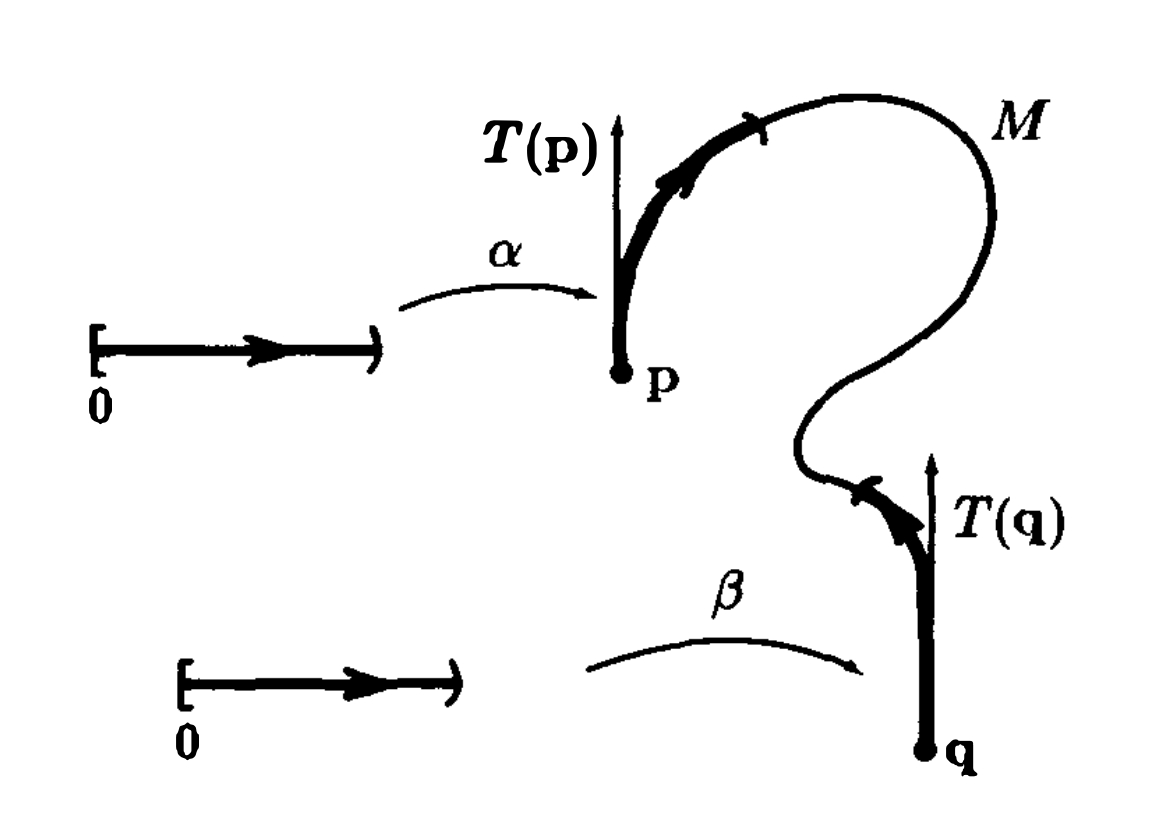
\includegraphics[scale=0.3]{images/Screenshot 2023-04-01 at 18.03.45.png}
    \end{figure}
    The problem disappears if we allow $U_2$ be open in $\mathbb{L}^1$. with this extra degree of freedom, it is easy to cover $M$ by coordinate patches that overlap positively. 
    \begin{figure}[H]
        \centering
        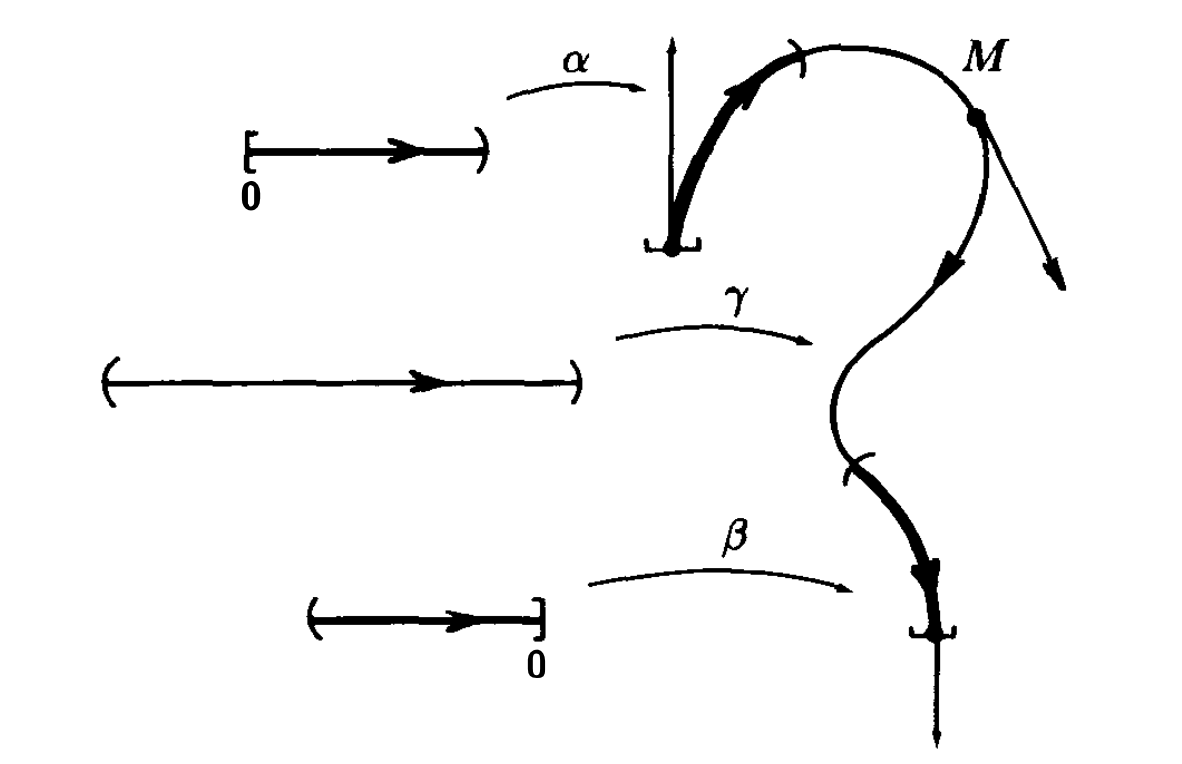
\includegraphics[scale=0.35]{images/Screenshot 2023-04-01 at 18.06.26.png}
    \end{figure}
\end{itemize}

\begin{theorem*}
    With this extra degree of freedom, every 1-manifold is orientable.
\end{theorem*}

\noindent\textbf{Remark}:
\begin{itemize}
    \item We now consider an arbitrary 1-manifold $M$ in $\R^n$. From basic topology, we can partition $M$ into connected components. We consider each component.
    \item If the component has no boundary, it looks like the first example. It has 2 orientations, one is cosidered to be like clockwise and the other is like counterclockwise.
    \item If the component has non-empty boundary, it looks like the second example. It also has 2 orientations, one is considered to be like going forward, and the other is like going backward.
    \item If 1-manifold $M$ has $k$ connected components, then it has $2^k$ orientations.
\end{itemize}

\begin{definition}
    Let $M$ be an (n-1)-manifold in $\R^n$. If $p\in M$, let $(p;n)$ be a unit vector in the n-dimensional vector space $\mathcal{T}_p(\R^n)$ that is orthogonal to the n-1 dimensional linear subspace $\mathcal{T}_p(M)$. 
    Then $n$ is uniquely determined up to sign. Given an orientation of $M$, choose a coordinate patch $\alpha:U\longrightarrow V$ on $M$ about $p$ belonging to this orientation. Let $\alpha(x)=p$. Then the columns $\frac{\partial \alpha}{\partial x_i}$ of the matrix $D\alpha(x)$ give a basis 
    $$\{(p;\frac{\partial \alpha}{\partial x_1}),\cdots,(p;\frac{\partial \alpha}{\partial x_{n-1}})\}$$
    for the tangent space to $M$ at $p$. We specify the sign of $n$ by requiring that the frame $$(n,\frac{\partial \alpha}{\partial x_1},\cdots,\frac{\partial \alpha}{\partial x_{n-1}})$$ be right-handed, that is, the matrix \begin{equation*}
        \begin{bmatrix}
            n & D\alpha(x)
        \end{bmatrix}
    \end{equation*}
    has positive determinant. $n$ is well-defined because we can show it is independent of the choice of $\alpha$. We can view $n$ as a function
    $$n:M\longrightarrow \R^n$$
    We can show that this function $n(p)$ is of class $C^{\infty}$. The vector field $$N(p)=(p;n(p))$$
    is called the \underline{unit normal field to $M$ corresponding to the orientation of $M$}.
\end{definition}

\noindent\textbf{Example}:
\begin{itemize}
    \item Consider the 2-manifold with boundary in $\R^3$ that looks like a weired bell which we saw before.
    \begin{figure}[H]
        \centering
        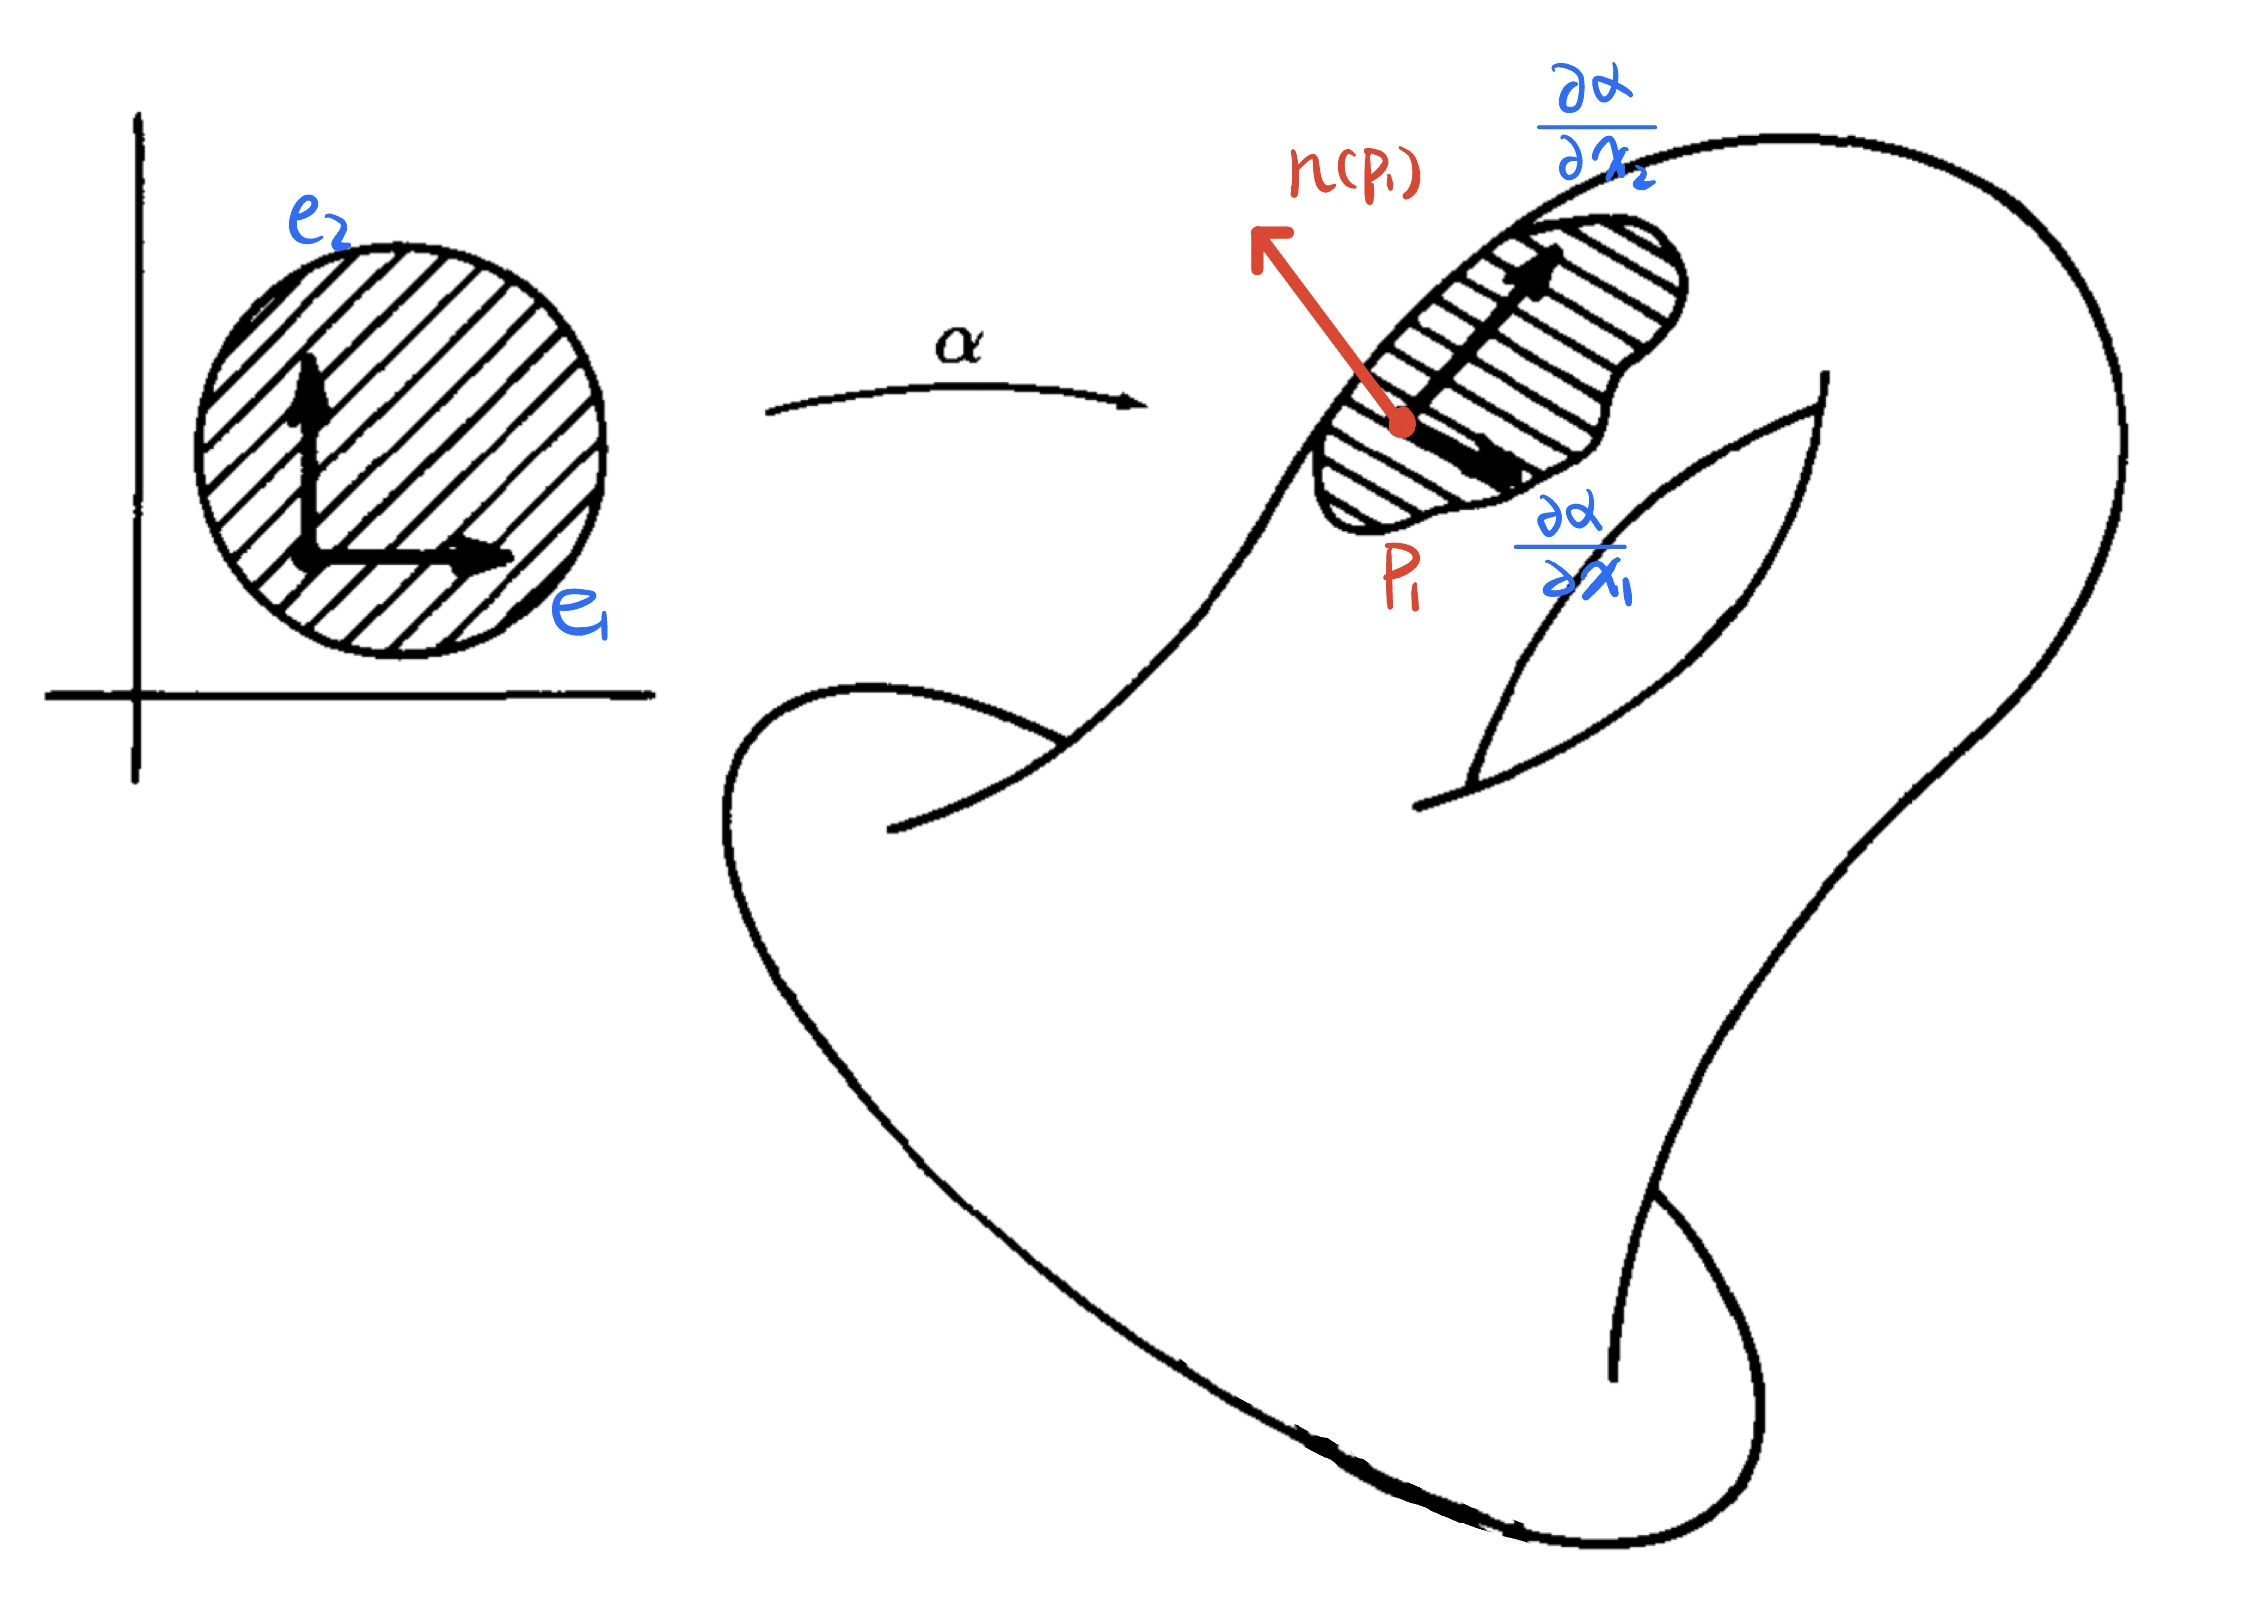
\includegraphics[scale=0.15]{images/IMG_0373.jpg}
    \end{figure}
    Consider the point $p_1$, the vector $n(p_1)$ is shown in the picture. Based on this orientation, for each point $p$, the vector $n(p)$ is pointing outward of the bell. 
    For the other orientation, $n(p)$ will pointing inside the bell. In this case, the two posiible orientations represent the outward of the manifold and the inward of the manifold.
    \item Consider $S^2$ in $\R^3$. Intuitively, this manifold also has two sides, inside and outside. Every point is like the above $p_1$.
    \item Now let us consider the famous Mobius band, which is a 2-manifold that can be embedded in $\R^3$. 
    \begin{figure}[H]
        \centering
        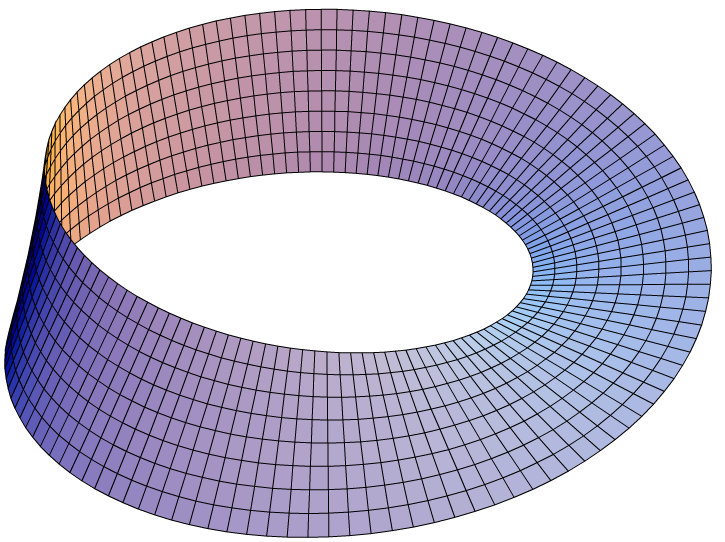
\includegraphics[scale=0.2]{images/Moebius_Surface_1_Display.png}
    \end{figure}
    This manifold is not orientable. Reason is simple, because all of us know that the mobius band only has one side! Rigorously, one can verify that we cannot have continuous unit normal vector field on the mobius band.
    Also from basic topology, we know that the Klein bottle is a 2-manifold that can be embedded in $\R^4$. Since it contains a copy of the mobius band, it is also not orientable. We will not give much details here. Everyone knows that the Klein bottle only has one side.
    \begin{figure}[H]
        \centering
        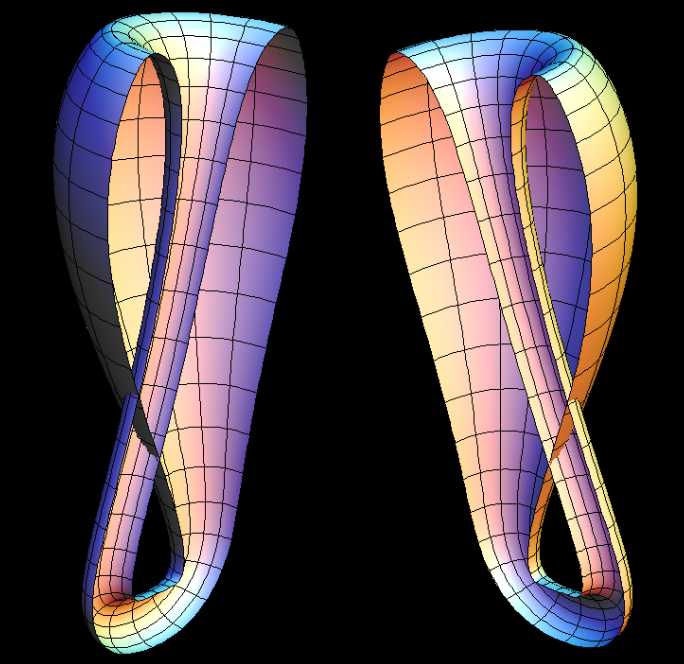
\includegraphics[scale=0.3]{images/kleinsymLR.png}
    \end{figure}
    Fun fact, we can stick two mobius bands along their edges to build a Klein bottle. This is a question on my topology final.
\end{itemize}

\begin{definition}
    Let $M$ be an n-manifold in $\R^n$. If $\alpha:U\longrightarrow V$ is a coordinate patch on $M$, then $D\alpha$ is an n by n matrix. 
    We define the \underline{nature orientation of $M$} to consist of all coordinate patches on $M$ for which $$\det(D\alpha)>0$$
    It is easy to see that two such patches overlap positively.
\end{definition}
\noindent\textbf{Remark}:
\begin{itemize}
    \item Consider $\alpha:U\longrightarrow V$, if $\det(D\alpha(x))<0$ for all $x\in U$, we need to apply the reflection map $$r(x_1,x_2,\cdots,x_n)=(-x_1,x_2,\cdots,x_n)$$
    Then $\alpha\circ r$ is the coordinate patch we want.
    Consider a 2-manifold in $\R^2$, the above can be shown in the picture
    \begin{figure}[H]
        \centering
        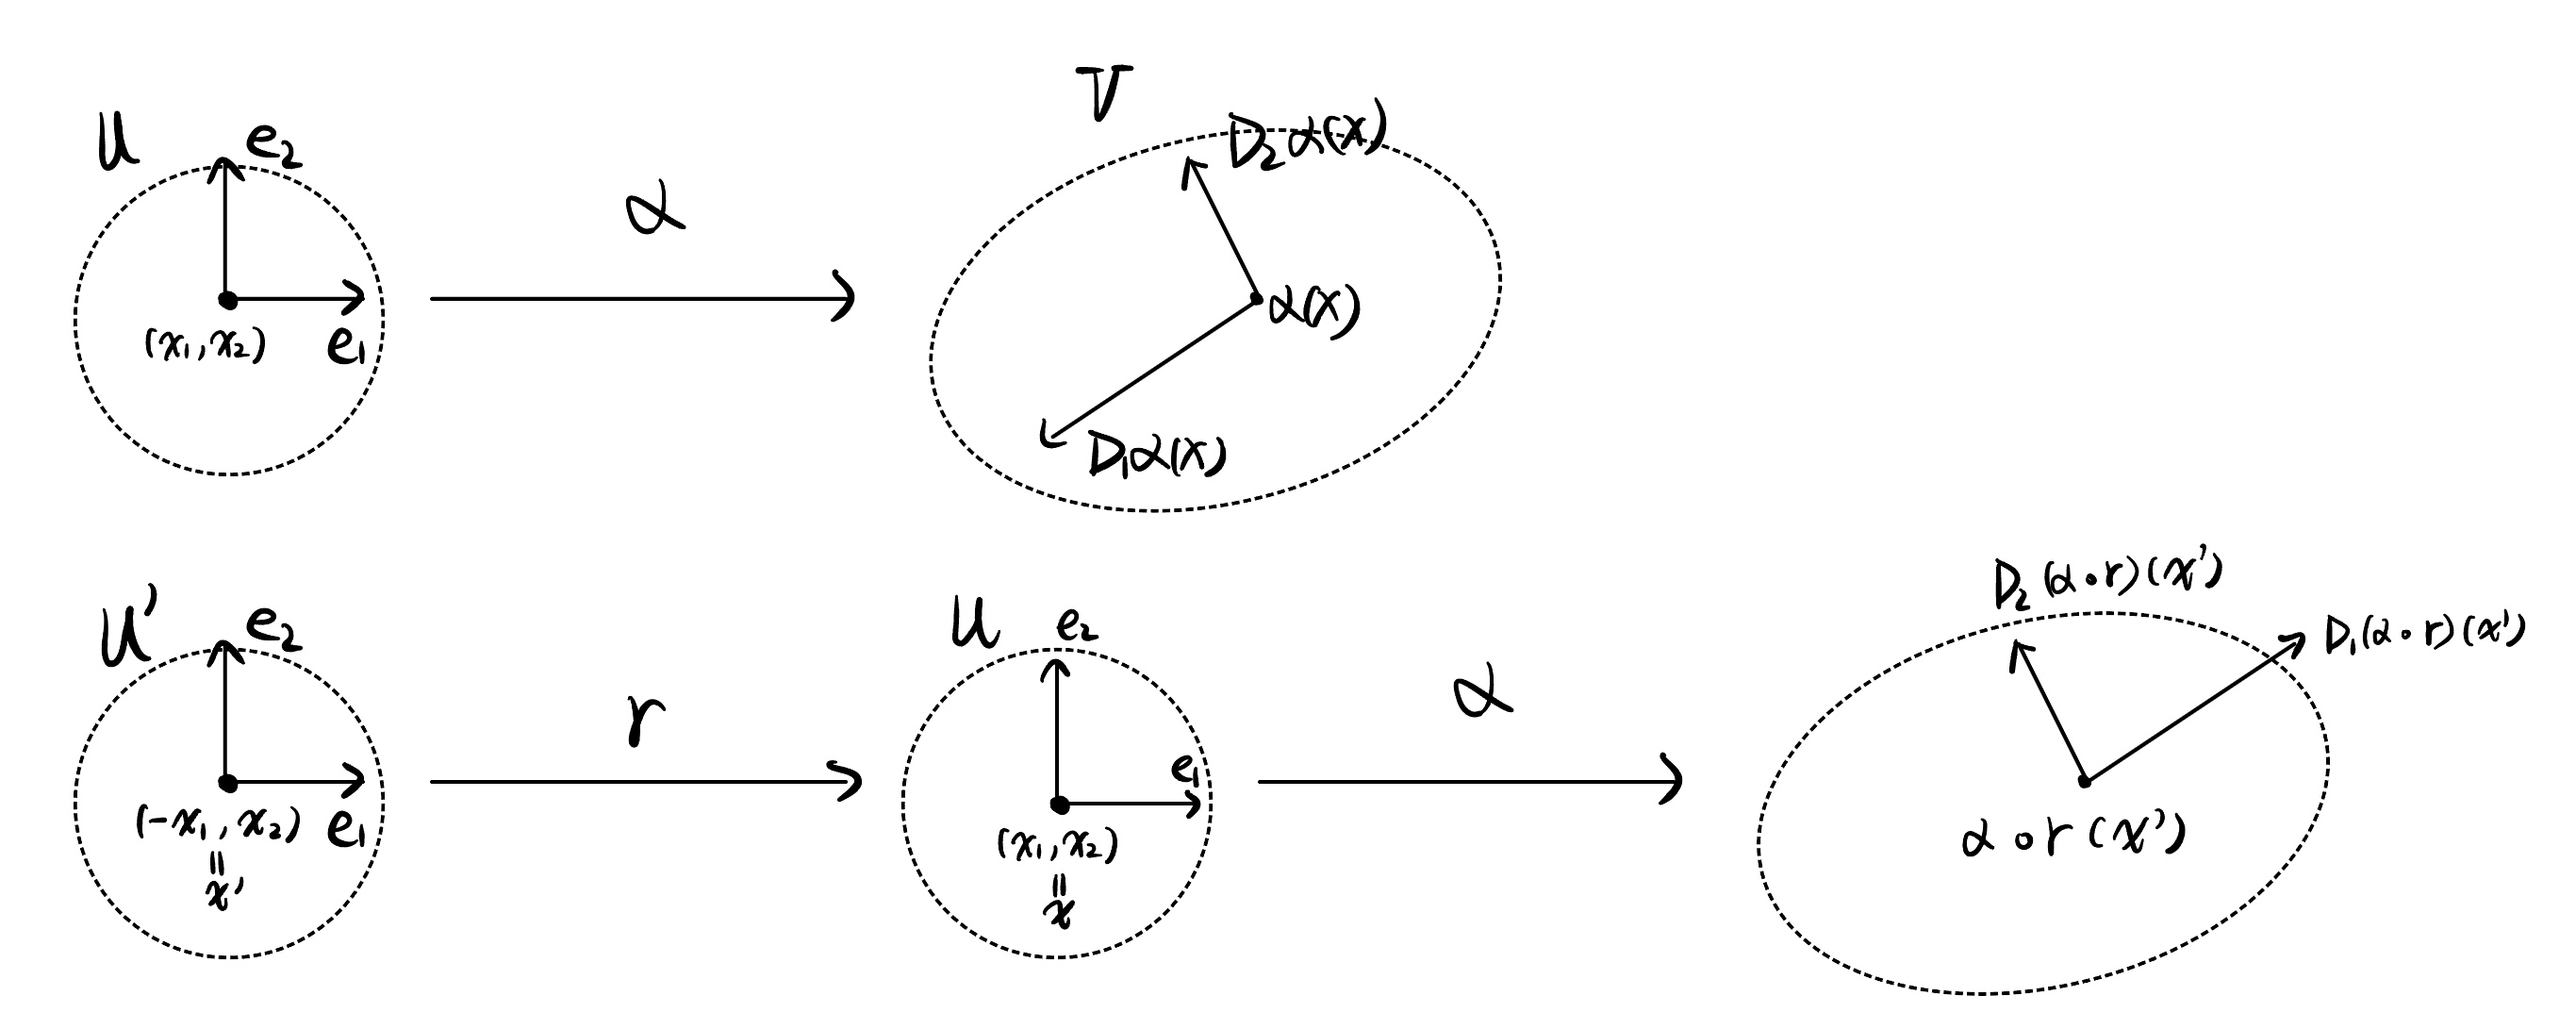
\includegraphics[scale=0.15]{images/IMG_0375.jpg}
    \end{figure}
    Notice that $$\alpha:U\longrightarrow V$$
    $$\alpha\circ r : U'\longrightarrow V$$
    where $U'$ is the open $U$ flipped along the y-axis. The above can be explained using the chain rule 
    \begin{equation*}
        \begin{split}
            D(\alpha\circ r)(x') &= D\alpha(r(x'))\cdot Dr(x')\\
            &= D\alpha(x)\cdot \begin{bmatrix}
                -1 & 0\\
                0 & 1
            \end{bmatrix}
        \end{split}
    \end{equation*}
\end{itemize}

\begin{definition}
    Let $M$ be an oriented k-manifold in $\R^n$. If $\alpha_i:U_i\longrightarrow V_i$ is a coordinate patch on $M$ belonging to the orientation of $M$. Let $\beta_i$ be the coordinate patches 
    $$\beta_i=\alpha_i\circ r: r(U_i)\longrightarrow V_i$$
    Then $\beta_i$ overaps $\alpha_i$ negatively, so it does not belong to the orientation of $M$. The coordinate pathches $\beta_i$ overlap each other positively, so they constitute another orientation of $M$. It is called the \underline{reverse or opposite} orientation to that specified by the coordinate pathches $\alpha_i$.
\end{definition}

\subsection{The Induced Orientation of $\partial M$}

\begin{theorem}
    Let $k>1$. If $M$ is an orientable k-manifold with non-empty boundary, then $\partial M$ is orientable.
\end{theorem}

\begin{definition}
    Let $M$ be an orientable k-manifold with non-empty boundary. Given an orientation of $M$, the corresponding \underline{induced orientation} of $\partial M$ is defined as follows: 
    \begin{itemize}
        \item If $k$ is even, it is the orientation obtaine by simply restriction coordinate patches belonging to the orientation of $M$.
        \item If $k$ is odd, it is the opposite of the orientation of $\partial M$ obtained in this way.
    \end{itemize}
\end{definition}

\noindent\textbf{Example}:
\begin{itemize}
    \item Consider a 3-manifold in $\R^3$ that is homeomorphic to the solid torus as shown in the picture. This is the case when $k=3$ which is odd. Consider the bottom point $p$ that is in the boundary. Let $$\alpha:U\longrightarrow V$$
    be the coordinate patch about $p$. $U$ is open in $\HH^3$.
    \begin{figure}[H]
        \centering
        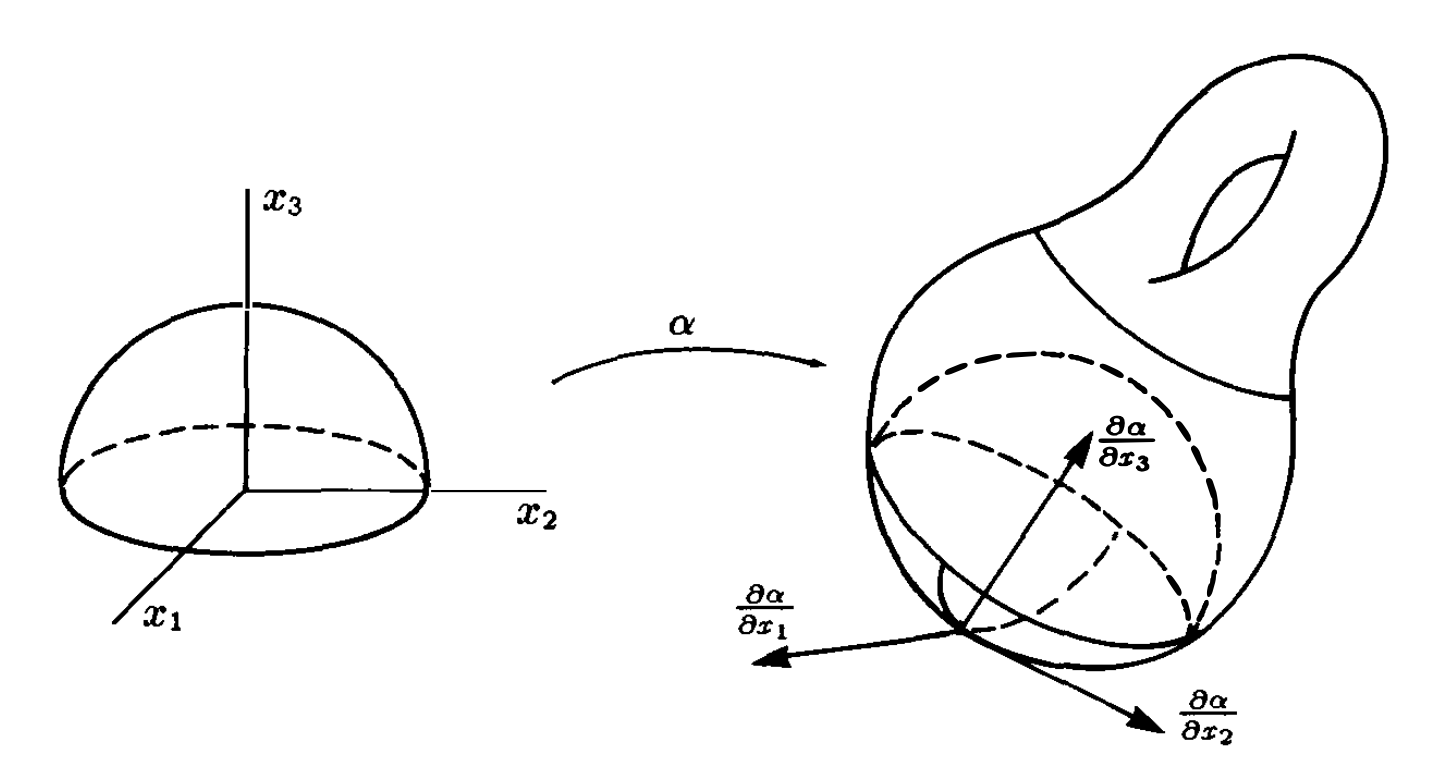
\includegraphics[scale=0.4]{images/Screenshot 2023-04-01 at 21.24.04.png}
    \end{figure}
    Now we restrict this coordinate patch to $\partial M$. $$\alpha|^{\partial M \cap V}:U'\longrightarrow V'$$
    where $U'\subset \R^2$ is the base of the half ball $U$ and $V'=\partial M\cap V$.
    $$\alpha|^{\partial M \cap V}(x_1,x_2)=\alpha(x_1,x_2,0)$$
    By the previous definition, we can assign a unit normal vector $n(p)$ such that $$(n(p),\frac{\partial \alpha|^{\partial M \cap V}}{\partial x_1},\frac{\partial \alpha|^{\partial M \cap V}}{\partial x_2})=(n(p),\frac{\partial \alpha}{\partial x_1},\frac{\partial \alpha}{\partial x_2})$$ is right-handed. But in here, we need the opposite, thus the normal field $$N(p)=(p;n(p))$$
    should have the property that $$(-n(p),\frac{\partial \alpha}{\partial x_1},\frac{\partial \alpha}{\partial x_2})$$ is right-handed. On the other hand, since $M$ is oriented naturally. It follows that 
    $$(\frac{\partial \alpha}{\partial x_3},\frac{\partial \alpha}{\partial x_1},\frac{\partial \alpha}{\partial x_2})$$ is right-handed. 
    It turns out that the orientation of $\partial M$ that corresponds to the unit normal field to $\partial M$ is pointing outwards.
    \item Now let us back to the weired bell that is a 2-manifold in $\R^3$. This is the case $k=2$ is even. 
    Consider the bottom point $p$ that is in the bouundary. Let $$\alpha:U\longrightarrow V$$
    be the coordinate patch about $p$. $U$ is open in $\HH^2$. 
    Let $N(p)=(p;n(p))$ be the unit normal field to $M$ corresponding to the orientation of $M$. 
    Let $T(p)=(p;\frac{D\alpha|^{\partial M\cap V}(t_0)}{\norm{D\alpha|^{\partial M\cap V}(t_0)}})$ be the unit tangent field to $\partial M$ corresponding to the induced orientation of $\partial M$. 
    The fun fact is that if you walk around $\partial M$ in the direction specified by $T$, with your head pointing in the direction specified by $N$, then the manifold $M$ is on your left.
    \begin{figure}[H]
        \centering
        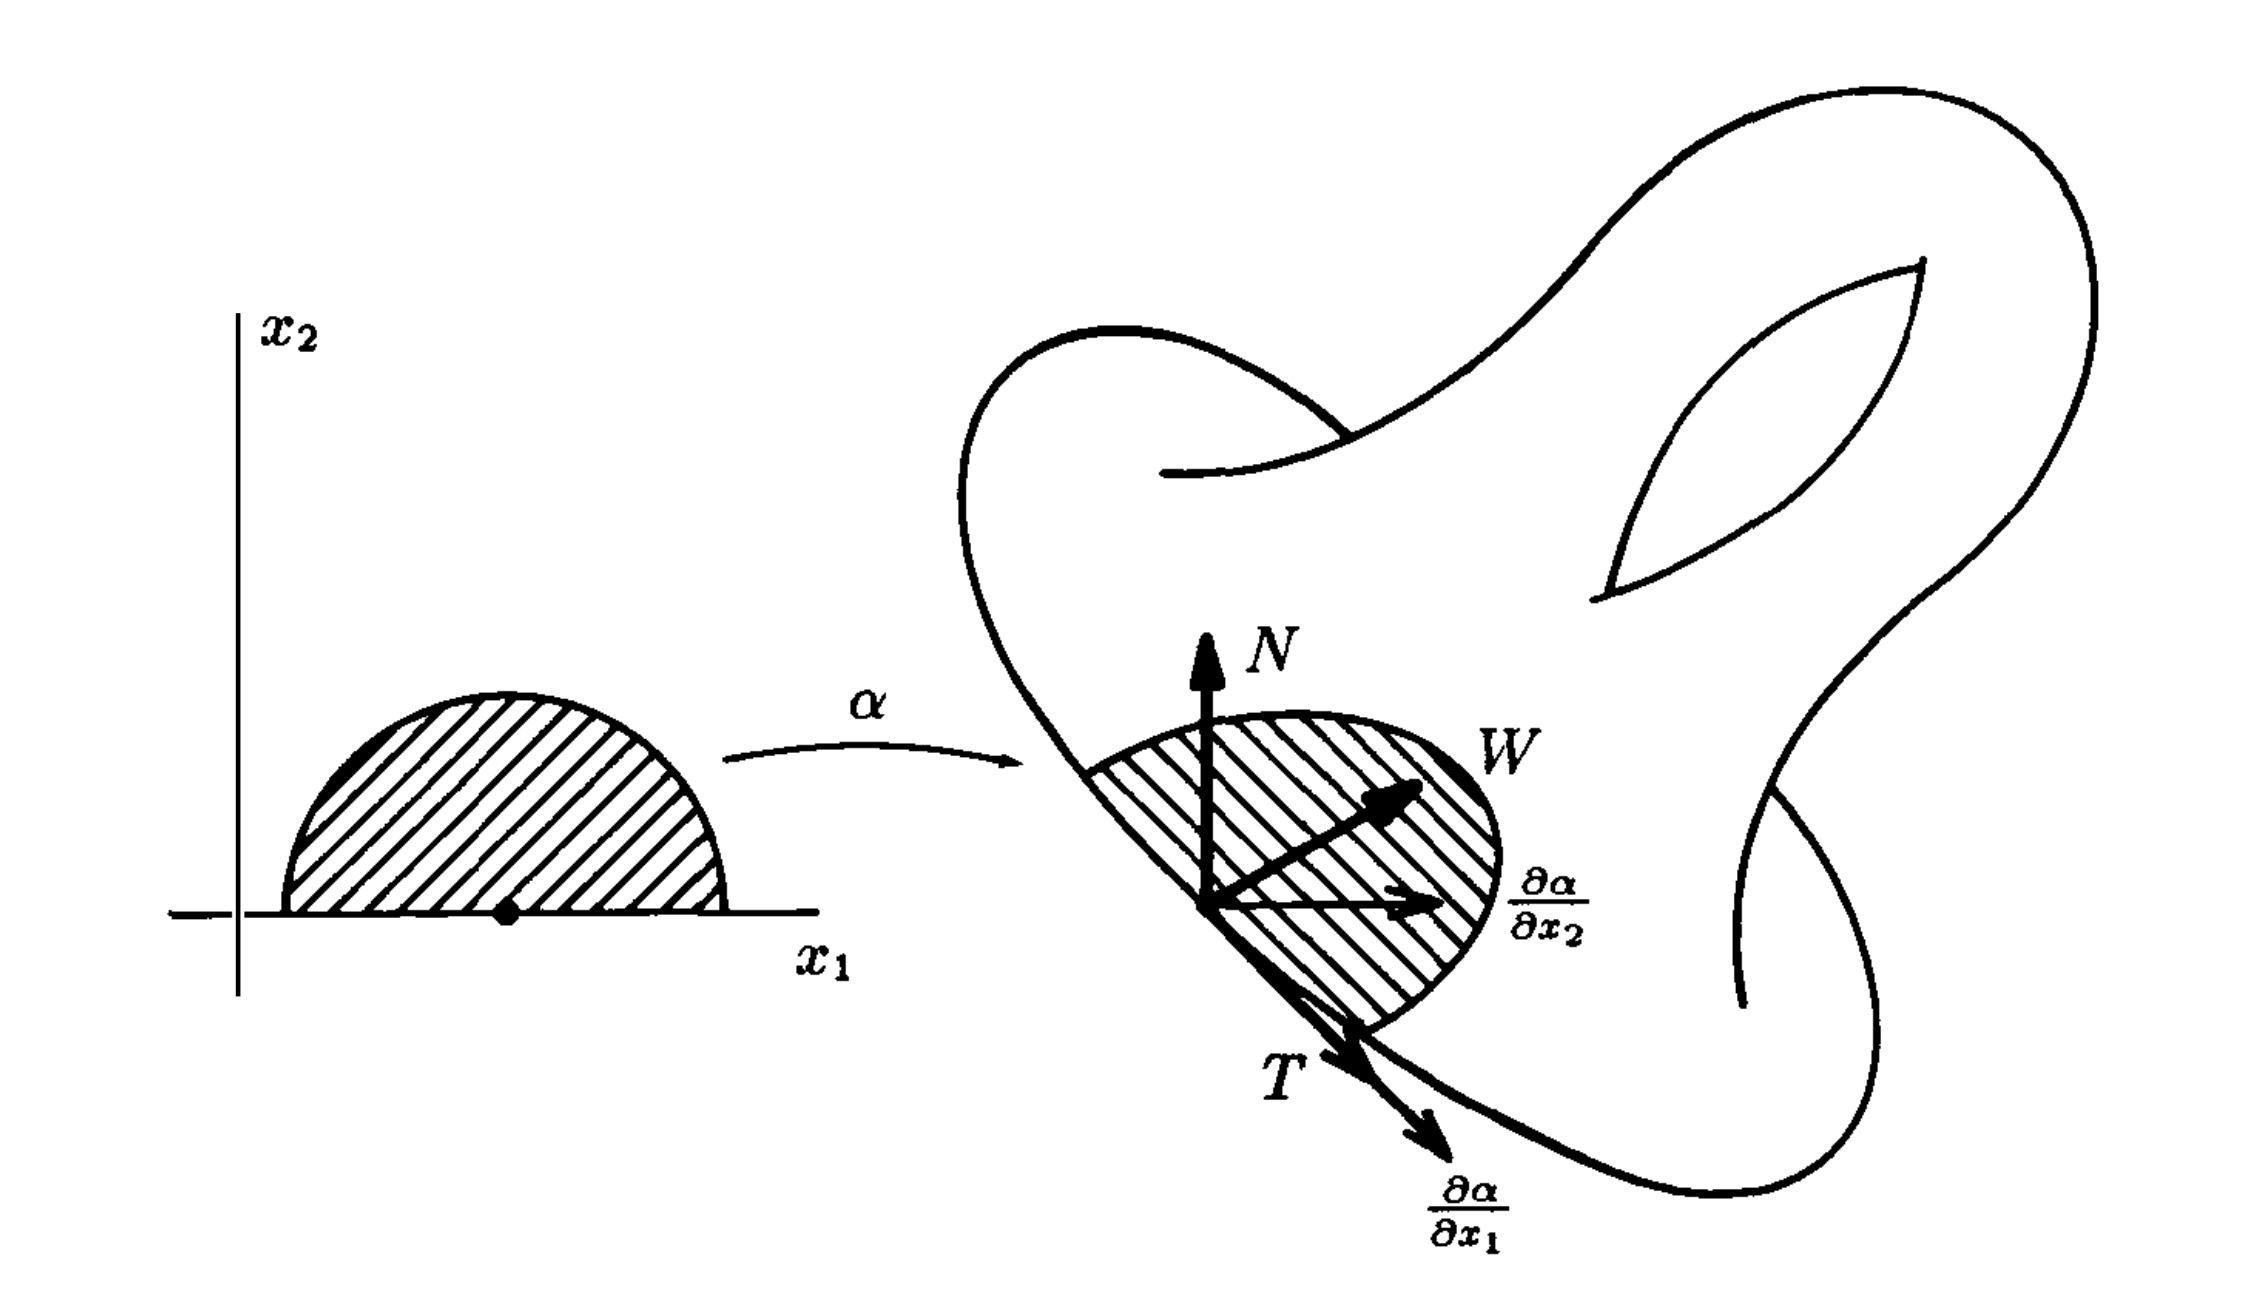
\includegraphics[scale=0.3]{images/Screenshot 2023-04-02 at 14.28.51.png}
    \end{figure}
    More precisely, let $W(p)=(p;w(p))$ that is perpendicular to both $N(p)$ and $T(p)$ such that $$(N(p),T(p),W(p))$$ is right-handed. Then $w(p)$ is tangent to $M$ at $p$ and points into $M$ from $\partial M$.
\end{itemize}

\section{Integrating Forms over Oriented Manifolds}

\begin{definition}
    Let $M$ be a compact oriented k-manifold in $\R^n$. Let $\omega$ be a k-form defined in an open set of $\R^n$ containing $M$. Let $C=M \cap supp(\omega)$. 
    Then $C$ is compact. Suppose there is a coordinate patch $\alpha:U \longrightarrow V$ on $M$ belonging to the orientation of $M$ such that $C\subset V$. By replacing $U$ by a smaller set if necessary, we can assume that $U$ is bounded. We define 
    the \underline{integral of $\omega$ over $M$} by the equation
    $$\int_M\omega=\int_{Int(U)}\alpha^*\omega$$
    Here $Int(U)=U$ is $U$ is open in $\R^k$, and $Int(U)=U\cap\HH^k$ if $U$ is open in $\HH^k$.
\end{definition}

\noindent\textbf{Remark}:
\begin{itemize}
    \item For the case $U$ is open in $\HH^k$, $\alpha$ can be extend to a $C^{\infty}$ map defined on $U'$ that is open in $\R^k$. So the form $\alpha^*\omega$ can be extended to a $C^{\infty}$ form on $U'$. This form can be written uniquely as $$\alpha^*\omega=h dx_1\wedge \cdots\wedge dx_k$$
    Therefore we have $$\int_{Int(U)}\alpha^*\omega=\int_{Int(U)}h$$
    \item The integral $\int_M\omega$ is well-defined, independent of the choice of the coordinate patch $\alpha$. Since now we choose $M$ to be an orineted manifold, we do not need to worry about the sign.
\end{itemize}

\begin{definition}
    Let $M$ be a compact oriented k-manifold in $\R^n$. we denote $-M$ as the manifold $M$ with the opposite orientation, then we have $$\int_{-M}\omega=-\int_M\omega$$
\end{definition}

\begin{definition}
    Let $M$ be a compact oriented k-manifold in $\R^n$. Let $\omega$ be a k-form defined in an open set of $\R^n$ containing $M$. Cover $M$ by coordinate pathches belonging to the orientation of $M$. 
    Then choose a partition of unity $\{\phi_1,\cdots,\phi_l\}$ on $M$ that is dominated by the coordinate patches on $M$. 
    We define the \underline{integral of $\omega$ over $M$} by the equation $$\int_M\omega=\sum_{i=1}^l[\int_M\phi_i\omega]$$
\end{definition}

\begin{theorem}[Linarity of integral of forms over oriented manifold]
    Let $M$ be a compact oriented mk-manifold in $\R^n$. Let $\omega$, $\eta$ be k-forms defined in anopen set of $\R^n$ containing $M$. Then $$\int_M(a\omega+b\eta)=a\int_M\omega +b\int_M\eta$$
    If $-M$ denotes $M$ with the opposite orientation, then $$\int_{-M}\omega=-\int_M\omega$$
\end{theorem}

\begin{theorem}
    Let $M$ be a compact oriented k-manifold in $\R^n$. Let $\omega$ be a k-form defined in an open set of $\R^n$ containing $M$. 
    Suppose $\alpha_i:A_i\longrightarrow M_i$ for $i=1,\cdots,N$, is a coordinate patch on $M$ belonging to the orientation of $M$, such that $A_i$ us open in $R^k$ and $M$ is the disjoint union of the open sets $M_1,\cdots,M_N$ of $M$ and a set $K$ of measure zero in $M$. Then $$\int_M\omega=\sum_{i=1}^N[\int_{A_i}\alpha^*\omega]$$
\end{theorem}

\section{A Geometric Interpretation of Forms and Integrals}

\begin{theorem}
    Let $W$ be a k-dimensional linear subspace of $\R^n$. 
    Let $(a_1,\cdots,a_k)$ be an orthonormal k-frame in $W$. 
    Let $f$ be an alternating k-tensor on $W$. 
    If $(x_1,\cdots,x_k)$ is an arbitrary k-tuple in $W$, then we have 
    $$f(x_1,\cdots,x_k)=\pm V(x_1,\cdots,x_k)f(a_1,\cdots,a_k)$$
    If the $x_i$ are independent and $(x_1,\cdots,x_k)$ and $(a_1,\cdots,a_k)$ belong to the same orientation of $W$, then the sign is $+$.
    If the $x_i$ are independent and $(x_1,\cdots,x_k)$ and $(a_1,\cdots,a_k)$ belong to the different orientation of $W$, then the sign is $-$. 
    If $x_i$ are dependent, then $V(x_1,\cdots,x_k)=0$ the sign does not matter. 
\end{theorem}

\begin{corollary}
    Let $(a_1,\cdots,a_k)$ and $(b_1,\cdots,b_k)$ be two orthonormal frames in $W$, then $$f(a_1,\cdots,a_k)=\pm f(b_1,\cdots,b_k)$$
    The sign depending on whether they belong to the same orientation of $W$ or not.
\end{corollary}

\noindent\textbf{Remark}:
\begin{itemize}
    \item Alternating tensors have geometric meanings, which can be seen in various contexts. Alternating tensors represent quantities that have a magnitude and orientation and are associated with area, volume, or higher-dimensional analogs.
    \item So given an alternating k-tensor on the vector space $W$, it tells us how to define a generalized volume.
\end{itemize}

\begin{definition}
    Let $M$ be a k-manifold in $\R^n$. If $M$ is oriented, then the tangent space to $M$ at $p$ has a natural induced orientation, defined as follows: 
    Choose a coordinate patch $\alpha:U\longrightarrow V$ belonging to the orientation of $M$ about $p$. Let $\alpha(x)=p$. The collection of all k-frames in $\mathcal{T}_p(M)$ of the form $$(\alpha_*(x;a_1),\cdots,\alpha_*(x;a_k))$$
    where $(a_1,\cdots,a_k)$ is a right-handed k-frame in $\R^n$. This collection is called the \underline{natural orientation} of $\mathcal{T}_p(M)$ induced by the orientation of $M$. 
    It is easy to show it is well-defined, independent of the choice of $\alpha$.
\end{definition}

\begin{theorem}
    Let $M$ be a compact oriented k-manifold in $\R^n$. Let $\omega$ be a k-form defined in an open set of $\R^n$ containing $M$. 
    Let $\lambda$ be a scalar function on $M$ defined by the equation $$\lambda(p)=\omega(p)((p;a_1),\cdots,(p;a_k))$$
    where $((p;a_1),\cdots,(p;a_k))$ is any orthonormal k-frame in the linear space $\mathcal{T}_p(M)$ belonging to its natrual orientation. Then $\lambda$ is continuous and $$\int_M\omega=\int_M\lambda \di V$$
\end{theorem}

\begin{theorem*}
    There exists a k-form $\omega_v$ defined in an open set about $M$ such that $\omega_v(p)$ on any orthonormal basis for $\mathcal{T}_p(M)$ belonging to its natural orientation is 1. 
    It is equivalent to say that $$\int_M\omega_v=\int_M\di V=v(M)$$
    The form $\omega_v$ is called a \underline{volume form for $M$}.
\end{theorem*}

\begin{corollary}
    Given any scalar function $\lambda$ on $M$, then we have $$\int_M\lambda\di V =\int_M\lambda\omega_v$$
\end{corollary}

\noindent\textbf{Remark}:
\begin{itemize}
    \item So back to the question how to understand differential forms? I think it tell us how to view the unit volume on the manifold.
\end{itemize}

\section{The Generalized Stokes' Theorem}

\begin{lemma}
    Let $k>1$. Let $\eta$ be a (k-1)-form defined in an open set $U$ of $\R^k$ containing the unit k-cube $I^k$. Assume that $\eta$ vanishes as all points of $Bd(I^k)$ except possibly at points of $Int(I^{k-1})\times 0$. Then 
    $$\int_{Int(I^k)}d\eta=(-1)^k\int_{Int(I^{k-1})}b^*\eta$$
    where $b:I^{k-1}\longrightarrow I^k$ is the map $$b(u_1,\cdots,u_{k-1})=(u_1,\cdots,u_{k-1},0)$$
\end{lemma}

\begin{theorem}[Stokes' Theorem for manifold of dimension $\geq 2$]
    Let $k>1$. Let $M$ be a compact oriented k-manifold in $\R^n$. 
    Give $\partial M$ the induced orientation if $\partial M$ is not empty. 
    Let $\omega$ be a (k-1)-form defiend in an open set of $\R6n$ containing $M$. Then 
    $$\int_Md\omega=\int_{\partial M}\omega$$
\end{theorem}

\begin{definition}
    Let $M$ be a 1-manifold in $\R^n$. Suppose there is a one-to-one map $\alpha:[a,b]\longrightarrow M$ of class $C^{\infty}$, carrying $[a,b]$ onto $M$ such that $D\alpha(t)\neq 0$ for all $t$. 
    Then we call $M$ a \underline{smooth arc} in $\R^n$. 
    If $M$ is oriented so that the coordinate patch $\alpha|_{(a,b)}$ belongs to the orientation, we say that $p$ is the \underline{initial point} of $M$ and $q$ 
    is the \underline{final point} of $M$.
    \begin{figure}[H]
        \centering
        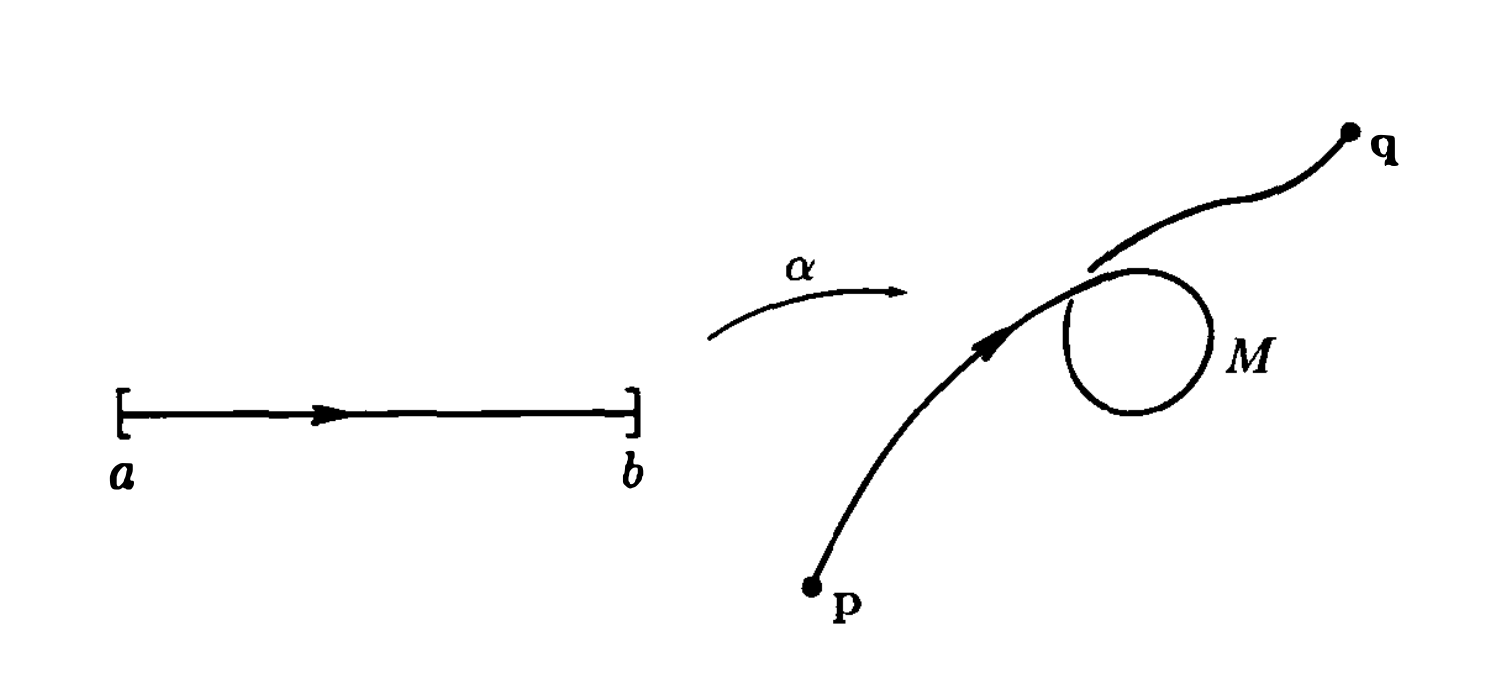
\includegraphics[scale=0.3]{images/Screenshot 2023-04-02 at 16.28.02.png}
    \end{figure}
\end{definition}

\begin{lemma}
    Let $M$ be a 1-manifold in $\R^n$. Let $f$ be a 0-form defined in an open set about $M$. If $M$ is an arc with initial point $p$ and final point $q$, then $$\int_Mdf=f(q)-f(p)$$
\end{lemma}

\begin{definition}
    A compact 0-manifold $N$ in $\R^n$ is a finite collection of points $\{x_1,\cdots,x_m\}$ of $\R^n$. 
    We defien an \underline{orientation of $N$} to be a function $$\epsilon:N\longrightarrow \{-1,1\}$$
\end{definition}

\begin{definition}
    If $M$ is an oriented 1-manifold in $\R^n$ with nnon-empty boundary, we define the \underline{induced orientation} of $\partial M$ by setting:
    \begin{itemize}
        \item If there is a coordinate patch $\alpha:U\longrightarrow V$ about $p\in\partial M$ belonging to the orientation of $M$ with $U$ open in $\HH^1$, we set $\epsilon(p)=-1$
        \item If there is a coordinate patch $\alpha:U\longrightarrow V$ about $p\in\partial M$ belonging to the orientation of $M$ with $U$ open in $\mathbb{L}^1$, we set $\epsilon(p)=1$
    \end{itemize}
    \begin{figure}[H]
        \centering
        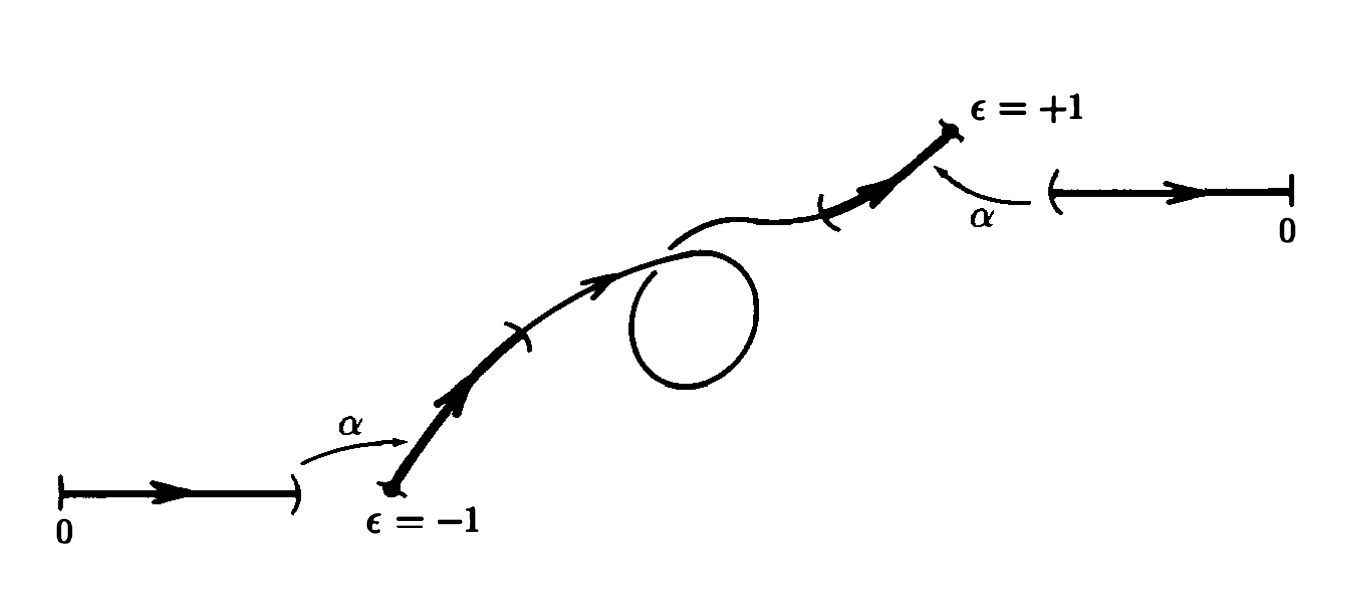
\includegraphics[scale=0.4]{images/Screenshot 2023-04-02 at 16.36.44.png}
    \end{figure}
\end{definition}

\begin{definition}
    let $f$ be a 0-form defined in an open set of $\R^n$ containing $N$, we define the \underline{integral of $f$ over oriented $N$} by $$\int_Nf=\sum_{i=1}^m\epsilon(x_i)f(x_i)$$
\end{definition}

\begin{theorem}{Stokes theorem for 1-manifold}
    Let $M$ be a compact oriented 1-manifold in $\R^n$. Give $\partial M$ the induced orientation if $\partial M$ is not empty. Let $f$ be a 0-form defined in an open set of $\R^n$ containing $M$. Then $$\int_Mdf=\int_{\partial M}f$$
\end{theorem}
\noindent\textbf{Remark}:
\begin{itemize}
    \item Recall the fundamental theorem of calculus, it is just the case when $n-1$ for this theorem!
\end{itemize}

\end{document}